\documentclass[suthesis,12pt,notitlepage]{report}
\usepackage{MyStyle}
\usepackage{suthesis}

\captionsetup{compatibility=false}


%\pdfoutput=1
\hbadness=10000

\begin{document}
	\Abstract{
		The era of gravitational waves astronomy was ushered in by the LIGO (Laser Interferometer Gravitational-Wave Observatory) collaboration with the detection of a binary black hole collision \cite{DetectionPaper}.  The event that shook the foundation of space-time allowed mankind to view the cosmos in a way that had never been done previously. Since then, another remarkable event was found by the LIGO and Virgo detectors where two neutron stars collided sending both gravitational and electromagnetic waves to earth \cite{BNS}. LIGO was built with the purpose of detecting the ripples in space-time caused by astrophysical events with the hopes of understanding the complexities hidden within the cosmos.  In 2011, the primary stages of Advanced LIGO were installed and commissioned to start the first observing run (O1).  During the writing of this thesis, the detectors had hardware replaced in order to mitigate noise from scattered light and new optics which reduced the losses from absorption.  The upgrades were in preparation for the third observing run (O3) and the work presented here is primarily focused on experimental techniques for operating at higher power and mode matching Gaussian beams in the dual-recycled Michelson interferometer for the Advanced LIGO era and beyond.  The first two chapters discuss the fundamentals of gravitational waves and the LIGO detector configurations.  The third chapter introduces the reader to fundamentals in mode matching Gaussian laser beams.  The fourth and fifth chapter summarizes the author's work at Syracuse University and LIGO Hanford observatory in mode sensing and high-powered commissioning.
	}
	
	\title{Adaptive Mode Matching in Advanced LIGO and Beyond}
	\author{Thomas V. Vo}
	\majorprof{Stefan Ballmer}
	% For the following line, if you got a masters, list it first. Otherwise, leave the first of the two entries blank, like the line below it.
	\previousdegree{M.S. Syracuse University, Syracuse, NY, 2016}{B.S. University of Washington, Seattle, WA, 2010}
	\submitdate{May 2019} % I know this says submit date, but SU requires that you put the month that you're going to graduate in.
	\degree{Doctor of Philosophy}
	\program{Physics}
	\copyrightyear{2019}
	\majordept{Physics}
	\haveminorfalse
	\copyrighttrue
	\doctoratetrue
	\figurespagetrue
	\tablespagetrue
	\electronicsubmittrue % if false, makes an approval title page. if true, makes title page with no approval spot. 
	%You need to submit a signed version of the approval title page to the office, then an electronic edition with no approval spot. this is dumb.
	
	\beforepreface
	\prefacesection{Preface}
	The work presented in this thesis stems from my participation in the LIGO
	Scientific Collaboration (LSC). This work does not reflect the
	scientific opinion of the LSC and it was not reviewed by the collaboration. 

	LIGO DCC Number: P1900086
	
	\prefacesection{Acknowledgements}
			I would like to thank my thesis advisor Stefan Ballmer for trusting in me as a scientist, always providing indispensable advice, and allowing me to follow my interests.
	
	To Peter Saulson: Your love of science truly inspires me to be a better scientist and teacher.
	
	To Duncan Brown:  Tough questions force us to grow and your group meetings provided a growth spurt.
	
	To Sheila Dwyer, Jenne Driggers, and Georgia Mansell: Thank you for your patience in teaching me the gritty details about the Hanford interferometer, I will never forget the in-chamber work at HAM6 and the long commissioning hours in the control room.
	
	To Daniel Sigg: Your dinners are the perfect fugue of flavors, conversations and friends. Thank you for letting me participate in some of the crucial interferometer commissioning tasks.
	
	To Keita Kawabe: Thank you for the tough questions but also the encouragement to do the best science.
	
	To Rick Savage: I was honored to be a Fellow for so long, thank you for the advice about all aspects of life and the fishing trips when I needed it most.
	
	To Aidan Brooks: Thank you for letting me work on/use TCS at Hanford, your guidance and experience is invaluable in times of confusion.
	
	To Daniel Vander-Hyde: Thank you for being patient with me when things weren't going well but also celebrating with me when things were!
	
	To Dan Brown: Cheers for coming across the pond to help when we needed it most and the Inbetweeners jokes on wings night.
	
	To Corey Gray, Gunner and Gomez: The hikes brought peace to my troubled mind and patience to my restless soul.
	
	To TJ Shaffer: Thank you for helping with steady hands or Guardian skills.
	
	To all the operators and staff at Hanford: Jeff, Betsy, Chandra, TJ, Jim, Cheryl, Nico, Patrick, Ed, Gerardo, Evan.
	
	To Hang Yu: Thank you for helping me understand the inner workings of the interferometer with only a few lines of math and a drawing.
	
	To my forever teachers Melissa Brainerd, Paul Didier, Chrissy Dahms, Carolyn West, and Dan Dorsey:  My work is a direct ripple from your teachings and you inspire kids like me from White Center to chase our dreams.
	
	To my childhood friends Quang, Leah, Thang, Sienna, Khanh, Truc, Kay, Tuan, Wanda, James, Matt and Trung:  You knew me when I was just dreaming of being a scientist, now we're here.
	
	To the Bloomingdale family: Thank you for making me feel at home even in the frigid Syracuse winters.
	
	To Jaysin Lord, Laura Nuttall, and Mat Hutchings: Thank you for the laughs and Thursday wings.
	
	To my family Cuong, Nhi, Tony, Theresa, Brittny, Kayla, Chloe: Your support and encouragement mean everything to me.
	
	To my parents: The difficulties of science are modest in comparison to your journey from Vietnam, this work is dedicated to you.
	
	To my darling Tiffany: Your support provides nourishment for my soul and your love gives a guiding light through the darkest of nights.
		
	\afterpreface
	

	
\chapter{Introduction}

	Say something profound here.
	
	Structure of this thesis:
	
		Gravitational waves and their detection
	
		The LIGO instrument and Noise + Squeezed States of Light
	
		Introduction to Wavefront Sensing
	
		Experimental Mode Matching at Syracuse
	
		Mode matching at LIGO Hanford
	
		Future Works

	\section{Gravitational Waves}\label{gravitational waves}
	In 1915, Albert Einstein published his theory of general relativity \cite{einstein}, which contains the most complete description of gravity to date. The seminal equation in this theory, called the Einstein Field Equation is
	
	\begin{equation} \label{einstein}
	G_{\mu \nu} = 8 \pi T_{\mu \nu}
	\end{equation}
	
	which is a set of 10 coupled second-order differential equations that are nonlinear and fully describes the interaction between space-time and mass-energy. Equation \ref{einstein} is difficult to solve except in situations where specific approximations allow a user to find exact solutions such as spherical symmetry \cite{carroll_2003} \cite{schutz_2009}. In areas where the curvature is close to flat,  the weak field approximation can be applied and the metric is described as	
	
	\begin{equation} \label{weak}
	g_{\mu \nu}  \approxeq \eta_{\mu \nu} + h_{\mu \nu}
	\end{equation}
	
	where $\eta_{\mu \nu}$ is the metric of flat space time and $|h_{\mu \nu}| \ll 1$ is the perturbation due to a gravitational field.
	
	By plugging in equation \ref{weak} into \ref{einstein} and using empty space we obtain the familiar wave equation
	
	\begin{equation} \label{wave}
	\Big(\nabla^2 - \frac{1}{c^2} \pdv[2]{t} \Big) h_{\mu \nu}  = 0
	\end{equation}

	which has a plane-wave solution of the form $h_{\mu \nu} = A_{\mu \nu} e^{ik_{\nu} x^{\nu}}$. 
	
	Using the gauge constraint $h^{\mu \nu}_{,\nu} = 0$, it follows that $A_{\mu \nu} k^{\mu} = 0$ which means that the gravitational wave amplitude is orthogonal to the propagation vector.
	
	Further imposing transverse-traceless gauge and assuming that the wave is traveling in the $x^3$ direction, it can be shown that the complex amplitude has physical significance expressed in the matrix
	
	\begin{equation} \label{gwamp}
	A_{\mu \nu} = 
	\begin{pmatrix}
			0 &    0   &  0      & 0 
		 \\ 0 & A_{xx} &  A_{yx} & 0
		 \\ 0 & A_{xy} & -A_{xx} & 0
		 \\ 0 &    0   &  0      & 0
	\end{pmatrix}
	\end{equation}

	Oftentimes, the four non-zero components of equation \ref{gwamp} can be categorized into two distinct polarizations called plus and cross such that $h_{+} = A_{xx} = -A_{yy}$ and $h_{\cross} = A_{xy} = A_{yx}$ .

 
	It is natural to attempt to understand the physical interpretation of equation \ref{gwamp} as an affect on the position of a free floating particle. Consider the four-velocity, $U^{\alpha}$, in the transverse traceless gauge where the coordinate itself is attached the particles and incorporates any small wiggles that would shake the coordinates.  Of course, any free particles will follow the geodesic equation
	
	\begin{equation}\label{geodesic}
	\nabla U^{\alpha} = \frac{\text{d}}{\text{d} \tau} U^{\alpha} + \Gamma^{\alpha}_{\mu \nu} U^{\mu} U^{\nu} = 0
	\end{equation}	
	where $\Gamma^{\alpha}_{\mu \nu} = \frac{1}{2} g^{\gamma \alpha}(g_{\gamma \mu, \nu} + g_{\gamma \nu,\mu} - g_{\mu \nu, \gamma} )$ are the famous Christoffel symbols.
	By evaluating the first term of the acceleration in equation \ref{geodesic},
	\begin{equation}\label{accel}
	\bigg(\frac{\text{d}U^{\alpha}}{\text{d}\tau}\bigg)_0 = -\Gamma^{\alpha}_{00} 
	\\ = \frac{1}{2} \eta_{\mu \nu} (h_{\beta 0, 0} + h_{0 \beta, 0} + h_{0 0, \beta} )
	\end{equation}
	However, comparing equation \ref{gwamp} and equation \ref{accel}, it is clear that if the particle is initially at rest, then a moment later it is still at rest! The term "at rest" is actually used liberally here since the coordinate system varies along with the gravitational wave. 
	
	Alternatively, one can ask if a gravitational wave passed by a pair of particles separated by length $L$, what would be the effect on the distance between two points?  The proper distance is defined as

	\begin{equation}\label{propdist}
	\delta l
	= \int{g_{\mu \nu} dx^{\mu} dx^{\nu}} \\
	= \int_{0}^{L}{g_{xx} {d}x}\\
	\approx |g_{xx}(x=0)|^{1/2}\\
	\approx [ 1 + \frac{1}{2} h_{xx}(x=0)] L
	\end{equation} 
	
	which shows us two very important points about the nature of gravitational waves.  Firstly, the effect is very small since the length variation, $h_{xx}$, is a small perturbation on flat space-time.  Secondly, the effect is proportional to the initial separation between the particles. This means a detector which is large will have a better chance to measure these small effects, an important point that drove the design of the Laser Interferometer Gravitational-Wave Interferometer (LIGO).
	
	\subsection{Measuring Gravitational Waves with Light}\label{measuringGWs}
	Even with the theoretical formulation of gravitational waves resolved by the 1970s \cite{PiraniPhysicalSignificance}, the possibility of detecting gravitational waves by ground-based instruments was still a controversial topic among scientists in the field \cite{CollinsGravity}.  During the famous Chapel Hill Conference in 1957 which included some of the great minds of the era such as Wheeler, Schwinger, and Feynman, the experimental search for gravitational waves began to take hold.  One thought experiment that was proposed by Feynmann \cite{SmootBrief} where he considered a bead sliding on a string with some friction as a gravitational wave passes by.  As the beads slide back and forth due to the wave described by equation \ref{propdist}, there will be some heat dissipated which means the gravitational wave must carry some energy.
	
	There is still the issue of an incredible amount of accuracy required to measure the strain from even the most dense astrophysical objects. The earliest attempts at detecting these small signals were famously done by Joseph Weber using large resonant bars and piezoelectric transducers to extract the energy from gravitational waves at the resonant frequencies of the bars. Picture of bar detectors at LHO.  However, these bars are limited by thermal noise and can only detect GWs in very narrow frequency bands. 
	
	Interferometers are devices that measure small displacements by using a laser that is split by a partially transmitting mirror (or beamsplitter), which allows 50$\%$ of the light to get reflected and 50$\%$ to be transmitted.  Each of the beams travel down the arms and reflect off of mirrors and return to the beamsplitter.  Upon reaching the optic, the two beams recombine and by the principle of superposition  the electromagnetic waves will add linearly at the output port (or antisymmetric port). Figure[].  The laser beams will gather phase as they propagate down each individual arm, and when recombining, the intensity of the light will be proportional to the phase differences between each beam.  This will correspond to a differential length that is described by
	
	\begin{equation}
	L_{-} = l_{x} - l_{y}
	\end{equation}
	
	As shown in equation \ref{propdist}, the effect of gravitational waves on the proper length between two free falling objects is proportional to the initial separation.  From figure[GWparticles], it is intuitively clear that interferometry would be an ideal technique to detect signals from a gravitational wave.  However, one can explicitly derive a ground-based interferometer's response to a GW from an astrophysical object.
	
	Consider a gravitational wave source arbitrarily located in the sky with respect to an interferometer on Earth. By denoting the interferometer's Cartesian coordinates as $\{\hat{x},\hat{y},\hat{z}\}$ with x and y located along the arms respectively such that the z-axis points directly towards the zenith (i.e. a right-handed system.).  Using the well known Euler angles, a relation from the detector frame to the source frame with coordinates $\{\hat{x}',\hat{y}',\hat{z}'\}$ can be seen in Figure[Euler]. 
	
	If a gravitational wave at the source has emitted GWs with plus and cross polarizations as denoted by equation \ref{gwamp}, then the detector time series can be regarded as \cite{S6sensitivity} \cite{Finn:1995}
	\begin{equation}
	h(t) = F_{+}(\theta,\phi,\psi) \, h_{+}(t) + F_{\times}(\theta,\phi,\psi) \, h_{\cross}(t)
	\end{equation}
	where $F_{+}(\theta,\phi,\psi)$ and $F_{\cross}(\theta,\phi,\psi$ are the antenna pattern functions that project the gravitational wave amplitudes onto the detector frame.
	
	\begin{equation}\label{Fplus}
	F_{+}(\theta,\phi,\psi) = -\frac{1}{2}[1+\text{cos}^2(\theta)] \text{cos}(2\phi) \text{cos}(2\psi) - \text{cos}(\theta) \text{sin}(2\phi) \text{sin}(2\psi)
	\end{equation}
	\begin{equation}\label{Fcross}
	F_{\cross}(\theta,\phi,\psi) = + \frac{1}{2}[1+\text{cos}^2(\theta)] \text{sin}(2\phi) \text{cos}(2\psi) - \text{cos}(\theta) \text{sin}(2\phi) \text{sin}(2\psi)
	\end{equation}
	
	If the gravitational wave is located directly above the interferometer such that $\theta = 0$ and setting $\psi=0$, then the magnitude of the antenna pattern is equal to unity.  Furthermore, by rotating about the $\phi$ angle such that the detector arms align with the plus polarization, the null geodesic equation (ie the path of a photon) in the interferometer frame becomes 
	
	\begin{equation}
	ds^2 = g_{\mu\nu}dx^{\mu} dx^{\nu} = -dt^2 + [1+h_{+}]  dx^2 + [1-h_{+}]  dy^2 + dz^2 = 0
	\end{equation}
	
	Now, if the photon is traveling along the x-arm, this means that $dy^2 = dz^2 = 0$ and the metric equation transforms to
	
	\begin{equation}
	\frac{dt}{dx} = \sqrt{ 1+h_{+} } \approx 1+\frac{1}{2} h_{+} 
	\end{equation}
	
	The amount of time required for the photon to reach the x-end mirror (starting at $t=0$) is equal to
	
	\begin{equation}\label{pathlength}
	t_1 = \int_{0}^{L_{x}} [1+\frac{1}{2}  h_{+}(x) ] \text{d}x
	\end{equation}
	
	where $L_x$ is the total length of the x-arm.  Upon returning to the beamsplitter, the photon's total time of flight for the x and y arms are, respectively,
	
	\begin{equation}
	t_2 = 2 L_x + \frac{1}{2} \int_{0}^{L_x} \bigg[  h_{+}(x) +  h_{+}(x + L_x)  \bigg] \text{d}x
	\end{equation}
	\begin{equation}
	t'_{2}= 2 L_y - \frac{1}{2} \int_{0}^{L_y} \bigg[  h_{+}(y) +  h_{+}(y + L_y)  \bigg] \text{d}y
	\end{equation}
	
	If the gravitational wave period is much longer than the time of flight, then $h_{+}$ does not change much during the measurement, which means $h_{+}(\eta_i) \approx h_{+}(\eta_i + L_{\eta_i}) \approx constant$.  By subtracting the flight times of the photons for each arm and setting $L = L_x = L_y$, the difference is proportional to the gravitational wave perturbation multiplied by the sum of arm lengths (with a factor of $c$ to get the units right),
	
	\begin{equation}
	\Delta t = t_2 - t'_{2} = \frac{2L}{c} h_{+}
	\end{equation}
	
	By recasting the expression for time of flight in terms of the phase picked up laser light as it travels through space, the differential phase shift is
	\begin{equation}\label{diffphase}
	\Delta \Phi = \Phi(t_{2}) - \Phi(t'_{2}) = \frac{4 \pi}{\lambda} \, h_{+} \, L
	\end{equation}
	
	The equation above is simple, however, it only works for gravitational wave signals that are not frequency dependent and it assumes that the path length can be arbitrarily long. Both points are actually not true \cite{Saulson} but we can alleviate these discrepancies by considering a gravitational wave signal of the form $h(t) = h_0 \text{exp} (i 2 \pi f_{GW} t)$  and repeating the calculation between equations \ref{pathlength} and \ref{diffphase}:
	
	\begin{equation}\label{gwsinc}
	\Delta \Phi (t) = h(t) \; \tau_{RT} \; \frac{2 \pi c}{\lambda} \; \text{sinc}(f_{GW} \tau_{RT}) e^{i \pi f_{GW} \tau_{RT}}
	\end{equation}
	
	where $\tau_{RT} = 2L/c$.  The response for a detector whose arm lengths are blank km have null points at the around blank Hz which means the instrument cannot be arbitrarily long, however, this point is not concerning because it is too expensive and difficult to make a terrestrial detector of this size.
	
	How to practically measure $\Delta \Phi$ with an interferometer is explained in section \ref{LIGOInstrument}.

	\subsection{Detection of Gravitational Waves}
	The purpose of LIGO is to observe gravitational waves emanating from astrophysical objects \cite{NSFproposal}, so it is natural to wonder how well a single detector can probe the universe.  It is worthwhile to explicitly derive the inspiral horizon distance, which is how far a single detector can see a source comprised two equal mass compact objects optimally oriented in the sky relative to the detector.  Signal-to-noise (SNR) is the level of interesting signals compared to the background noise, which can be expressed as
	\begin{equation}\label{SNR}
	\rho = 2 \int_{-\infty}^{\infty} \frac{ \tilde{s}(f) \tilde{s}^*(f) }{S_n(f)}
	\end{equation}
	
	where ${S_n(f)}$ is the one-sided average power spectral density of the detector noise and $\tilde{s}(f)$ is the Fourier transform of the detectors' response to a gravitational-wave signal.
	
	Consider two dense objects with mass $m_1$ and $m_2$ rotating around each other, separated by a distance $R$ such that quadrupole equation still holds (i.e. flat space-time with small perturbations). The detector response, in units of strain, to the gravitational waves emitted by this source is \cite{Finn:1995},
	
	\begin{equation}\label{inspiralsignal}
	s(t) = \frac{\mathcal{M}}{d_L} \Theta(\theta,\phi,\psi,i) [\pi f(t) \mathcal{M}]^{2/3} \cos[\Phi(t) + constant]
	\end{equation}
	where 

	\begin{subequations}
		\begin{equation}\label{chirp}
	\mathcal{M} \&= (1+z) \frac{(m_1 m_2)^{3/5}}{(m_1 + m_2)^{1/5}}
		\end{equation}
		\begin{equation}\label{orient}
	\Theta(\theta,\phi,\psi,i) \&= 2 \sqrt{	[F_{+}(\theta,\phi,\psi) (1+\cos^2(i)) ]^2 + [2 F_{\cross} \cos(i)]^2 }
		\end{equation}
	\end{subequations}

	By convention, $\mathcal{M}$ called the chirp mass and $d_L$ is the luminosity distance. The orientation response, $\Theta(\theta,\phi,\psi,i)$, is a function that depends entirely on the detector orientation relative to the angular momentum vector of the binary [Figure of a binary spiraling and a detector on earth]
	
	
	where $F_{+}$ and $F_{\cross}$ are from equation \ref{Fplus} and \ref{Fcross}.
	
	As the binary loses energy to gravitational waves, the orbit will shrink as a function of time, in turn, the orbital frequency will increase
	
	\begin{equation}
	f(t) = \frac{1}{\pi \mathcal{M}} \bigg[\frac{5}{256} \frac{\mathcal{M}}{T-t}\bigg]^{3/8} 
	\end{equation}
	
	By defining the binary phase as $f(t) = \frac{1}{2\pi} \frac{\partial \mathbf{\Phi} }{\partial t}$, it is easy to recognize that the phase also evolves with time.
	\begin{equation}
	\Phi(t) = 2\pi \int_{T}^{t} f(t) dt = -2 \bigg( \frac{T-t}{5\mathcal{M}}\bigg)^{5/8}
	\end{equation}
	
	What this means is that the gravitational wave signal from the binary will increase in amplitude and frequency as a function of time up until the coalescence time, $T$.


	There is actually a subtle difference between the coalescence time and the moment when adiabatic approximations fail which allows usage of the quadrupole formulation. 

	Plugging equation \ref{inspiralsignal} into \ref{SNR},
	\begin{equation}
	\rho = 8 \Theta(\theta,\phi,\psi,i) \frac{r_0}{d_L} \bigg(\frac{\mathcal{M}}{1.2 \textup{M}_\odot}\bigg)^{5/6} \zeta(f_{max})
	\end{equation}
	
	There are two important functions in the equation above that reflect the detector's performance in sensing gravitational radiation from a binary inspiral, $r_0$ and $\zeta(f_{max})$.
	
	The characteristic distance, $r_0$ is how far the detector can see for a fixed binary's mass distribution,
	
	\begin{equation}\label{char_r0}
	r_0^2 = \frac{5}{192\pi^{4/3}} \bigg(\frac{3\textup{M}_\odot}{20}\bigg)^{5/3}   \int_{0}^{\infty} \frac{1}{S_n(f)} \frac{\text{d} f}{f^{7/3}}
	\end{equation}

	Due to the integrand's dependence on $f^{-7/3}$, lower frequency improvements in the detector's noise spectrum will contribute more to the distance.
	
	\begin{equation}\label{zeta}
	\zeta(f_{max}) = \frac{\int_{0}^{2f_{max}} \frac{1}{S_n(f)} \frac{\text{d} f}{f^{7/3}}}{\int_{0}^{\infty} \frac{1}{S_n(f)} \frac{\text{d} f}{f^{7/3}}}
	\end{equation}
	
	The sensitivity can be different for various mass distributions; $\zeta(f_{max})$ is a normalized function that describes how well the detector's bandwidth overlaps the binary's frequency evolution.  If $f_{max}$ is higher that the minimal sensitivity frequency for the detector, then there is good overlap and  $\zeta(f_{max})\approx 1$.  However, if the masses are sufficiently large, $f_{max}$ will be lower because coalescence occurs before the objects reach a higher frequency regime and this will result in  $\zeta(f_{max})\approx 0$.
	
	The process of two objects coalescing starts at lower frequencies and terminate at some $f_{max}$ that depends on when the objects reach their inner-most stable circular orbit, $f_{ISCO}$.   If $m_1=m_2$, then the maximum frequency is[]
	
	\begin{equation}
	\begin{aligned}
	f_{max}	=&  \frac{f_{ISCO}}{1+z} \\
			=&	\frac{99 \text{Hz}}{1+z} \, \frac{20 \textup{M}_\odot}{M}
	\end{aligned}
	\end{equation}
	where $M=m_1+m_2$.
	
	
	By plugging a few mass distributions and an estimate of the sensitivity [GWINC], it is possible to study the range of a single detector.  For example, a 1.4-1.4$\textup{M}_\odot$ binary that has optimal orientation with respect to the detector has horizon distance equal to...
	
	Horizon distance and range, advanced LIGO projected
	
	[Finn, Duncan Thesis]
	\cite{Saulson}
	
	\section{The LIGO Instrument}\label{LIGOInstrument}
	In its simplest form, the LIGO instrument is an incredibly large Michaelson interferometer.  
	If we imagine the output as a measure of differential arm lengths, it becomes a natural way of detecting gravitational waves. However, to make a practical gravitational-wave observatory, the complexity will have to be extended beyond what Michelson and Morley used.  
	The next sections will explore the various upgrades to the instrument configuration that improve the sensitivity of LIGO.
	
		\subsection{Simple Michaelson}\label{michelson}
		As shown in Figure [michelsonifo], the interferometer readout uses a photodetector that measures the total laser beam power and depends on how light in the arms constructively or destructively interferes at the beamsplitter. 
		In Section \ref{measuringGWs}, it was shown that the differential time of flight between photons traveling down the individual arms carry gravitational wave information.  
		The difference in flight times, $\Delta t$, can be converted into how much phase, $\Delta \phi$, is accumulated by the photons as they propagate through space.  
		But the question remains how an interferometer actually measures $\Delta \phi$.
		
		If the input electric field of the interferometer is $E_0$, the beamsplitter will transmit $E_0 /2$ down the x-arm and reflect $E_0 /2$ down the y-arm.  By setting the beamsplitter to be the origin, the two plane waves traveling down their respective arms will have gathered a phase $\phi_i$. Then, upon reflecting off the end mirrors and returning to the beamsplitter, each of the electric fields can be described by these equations
			\begin{equation}
			\begin{aligned}
				E_{x} 	&=	\frac{i E_0}{2} e^{2i\phi_{x}}	
			\\	E_{y} 	&=	\frac{i E_0}{2} e^{2i\phi_{y}}
			\end{aligned}
			\end{equation}
		Since the electromagnetic waves are linear, the resultant sum of waves at the antisymmetric port will be $E_{out} = E_x + E_y$. A photodiode (PD) is placed at the output (or antisymmetric) port to read out the integrated power which is related to the total electric field by
			\begin{equation}
			\begin{aligned}\label{asy_power}
				P_{AS}	&= \int_{\text{Area}} I \;				\text{d}A 
			\\			&= \int_{\text{Area}} \vert E_x + E_y \vert^2 \;	\text{d}A 
			\\			&= P_{in} \; \cos^2(\Delta \phi)
			\end{aligned}
			\end{equation}	
		where $\Delta \phi = \phi_{x} - \phi_{y} = k_x L_x - k_y L_y$ and $P_{in} = \int_{\text{Area}}	 \vert E_0\vert^2 \text{d}A$ is the input power. By using equation \ref{diffphase} and the common (or average) arm length $L_{+} = \frac{L_x + L_y}{2}$, the power due to a differential phase shift is
			\begin{equation}
			P_{AS} \approx P_{in} \; (1-2 \Delta \phi) = P_{in} \; (1-2 k L_{+} h_{+})
			\end{equation}
		There is a large DC term that is dependent on the input power and generally, it is very difficult to measure small changes in a large signal. So the next obvious method would be to shift the arms such that the output port is operating on a dark fringe, normally this is called a null-point operation.  However, there are difficulties associated with this method as well.  
		Consider shifting the phase of equation \ref{asy_power} by $\pi/2$, which would result in
			\begin{equation}\label{null}
			P_{AS} \vert_{null} = P_{in} \; \text{sin}^2 (\Delta \phi) \approx P_{in} \; (k L_{+} h_{+})^2 
			\end{equation}
		This results in a second-order dependence on a gravitational-wave signal that is already approximated to be very small.  
		So a good solution to the issue of how to $read$ out a gravitational wave signal can be solved using radio frequency (RF) detection methods. Consider changing the interferometer input by adding an electro-optical modulator (EOM) to sinusoidally modulate the laser frequency and expanding to first order using the Bessel functions,
			\begin{equation}\label{modE}
			\begin{aligned}
			E_{in} 	&= E_{0} e^{i(wt + \beta \text{cos} (\Omega t))} \\
					&\approx E_0 e^{iwt} [J_0(\beta) + J_1(\beta) e^{i \Omega t} + J_1(\beta) e^{-i \Omega t}] \\
					&= E_{C,in} + E_{SB+,in} + E_{SB-,in}
			\end{aligned}
			\end{equation}
		where $\Omega$ and $\beta$ are the modulation frequency and depth, respectively. The first term is commonly called the carrier field whereas the second and third terms are referred to as the (upper or lower) sidebands.  Because there are multiple electric fields, it is useful to define an optical transfer function which transforms the interferometer's input fields to its output,
		\begin{equation}\label{opt_tf}
		E_{out} = E_{C} + E_{SB+} + E_{SB-} = 
		\begin{pmatrix}
			t_{C} 	&   
		\\ 	t_{SB+} &
		\\ 	t_{SB-} &
		\end{pmatrix}
		\begin{pmatrix}
		E_{C,in} &    E_{SB+,in}    &  E_{SB-,in}     
		\end{pmatrix}
		\end{equation}
		The carrier transfer function, $t_{C}$ has already been calculated by equations \ref{asy_power} - \ref{null} and the sideband transfer functions are not much different.
		\begin{equation}\label{sb_tf}
		t_{SB\pm} = r_{x,\pm}  e^{i\phi_{\pm,x}} - r_{y,\pm}  e^{i\phi_{\pm,y}}
		\end{equation}
		where $\phi_{\pm,i} = (k \pm k_{\Omega}) \, \ell_{i} = (\frac{w+\Omega}{c} ) \ell_{i}$. In the current example, the sidebands and carrier fields reflect off the end mirrors identically, however, this will not be true in general when dealing with resonators that are highly frequency dependent.  Plugging equation \ref{sb_tf} into \ref{opt_tf}, the output electric field becomes 
		\begin{equation}
		E_{out} = i e^{iwt} [ J_0(\beta) 	k \ell_{+}  h_{+}  \; + \; J_1(\beta) \sin( k \Delta \ell + k_{\Omega} \Delta \ell) (e^{i\Omega t}  + e^{-i\Omega t}) ]
		\end{equation}
		By choosing the carrier signal to be on the dark fringe, $k \Delta \ell = \pi/2$ but the sidebands to be slightly off the null (Figure []) and hence leak into the anti-symmetric port, the electric field reduces to
		\begin{equation}
		E_{out} = i e^{iwt} [ J_0(\beta) 	k \ell_{+}  h_{+}  \; + \; J_1(\beta) \sin(k_{\Omega} \Delta \ell) ( e^{i\Omega t} + e^{-i\Omega t}) ]
		\end{equation}
		
		Recall that the intensity is equal to the electric field squared,
		\begin{equation}\label{RFdet}
		\begin{aligned}
			I	= \vert E_{out} \vert^2  =	&\vert E_{C}\vert^2 + \vert E_{SB+}\vert^2 + \vert E_{SB-}\vert^2 \\
										  	& + 2 \mathbf{Re} \{ \; E_{SB+} E^*_{SB-} e^{2i\Omega t} \; \}\\
										  	& + 2 \mathbf{Re} \{ \; (E_{C} E^*_{SB-} +  E_{SB+} E^*_{C} ) e^{i\Omega t} \; \}
		\end{aligned}
		\end{equation}
		The last term is referred to as the $beat$ $note$ between the carrier signal and the sidebands.  It is possible to extract the term at the modulation frequency using a mixer which is an analog device that outputs the product of two inputs. Usually, the same oscillator that was used to modulate the input beam can be one of the mixer inputs, $\cos(\Omega t)$,  so that the demodulated signal is
		\begin{equation}
		\begin{aligned}
		I_{Demod} 	&\propto \big[ 4 \pi  J_0(\beta) J_1(\beta) \frac{\ell}{\lambda}  \sin(k_{\Omega} \Delta \ell)  \; h_{+}\big] \big[ \cos(\Omega t)  \sin(\Omega t + \phi_{Demod}) \big] \\
					&\propto \big[ 4 \pi  J_0(\beta) J_1(\beta) \frac{\ell}{\lambda}  \sin(k_{\Omega} \Delta \ell)  \; h_{+}\big] \big[ \sin(\phi_{Demod}) + \sin(2\Omega t + \phi_{Demod}) \big]
		\end{aligned}
		\end{equation}
		where $\phi_{Demod}$ is the phase that can be set by the user in order to account for extra phase shifts (ie. longer cables). After the mixer, there will be signals at DC, $\Omega$, $2\Omega$ and so on. However, the part that is linear in the gravitational wave amplitude will be at DC so a low-pass filter will allow the final signal to dominate:
		\begin{equation}
		S = 4 \pi  J_0(\beta) J_1(\beta) \frac{\ell}{\lambda}  \sin(k_{\Omega} \Delta \ell) \sin(\phi_{Demod}) \; h_{+}
		\end{equation}
		This shows that a RF detection technique will be linear in GW signal with no large DC offset. Setting the carrier on a null point means $\Delta \ell = \frac{k_{\Omega}}{k} \frac{\pi}{2}$ and allows the designer to optimize the Schnupp asymmetry length to get the best signal for some modulation frequency. This type of readout scheme was used in Enhanced LIGO and is called heterodyne detection, where the sideband fields are produced by an EOM and its efficacy depends on the local oscillator's stability \cite{FritschelReadout}.  
		In contrast, the Advanced LIGO scheme uses a homodyne detection \cite{HildDCReadout} method called "DC-Readout".  Here the oscillator field is produced by slightly offsetting the arms away from the dark fringe and letting a small amount of carrier light through the antisymmetric port.  A gravitational wave will induce sidebands on the carrier and this will allow the same mathematics as above to achieve a linear signal in gravitational wave strain. This method benefits from naturally being co-aligned and mode matched with the signal field.  All techniques follow the same logic of beating the field containing useful information with a reference field to extrapolate a linear signal but the differences come from technical noise such as laser intensity fluctuations and effective quantum noise.
		
		\cite{BlackPDH}	
	
		\subsection{Fabry-Perot Cavities}\label{FP}
		There are two ways to improve the LIGO detectors: one is to increase the response from gravitational waves and the other is to decrease the noise contributions. From equation \ref{diffphase}, the gravitational wave signal is proportional to the optical path length that the photon travels, which means the most straightforward method of increasing the sensitivity is to make the arms as long as possible (up to the null point described by equation \ref{gwsinc}.  Generally, there were two methods to do this: a Herriott delay line or a Fabry-Perot resonator, the differences between each method is shown in Figure[].  At the time of writing this thesis, all modern gravitational wave detectors use the latter method.
	
		A Fabry-Perot cavity is an optical system comprised of two or more partially transmitting mirrors with one laser input.  To create a resonator, the user must design a system such that once the laser has made one round trip around the optics, it is the same shape and size as when it started.  Conceptually, this may seem simple but in practice, controlling and sensing any optical cavity comes with a few challenges.
		
		To start understanding the longitudinal degree of freedom, consider a two mirror system in Figure [] which is separated by a length $L$ with reflection and transmission coefficients: $r_1$, $t_1$, $r_2$, $t_2$.	
		Starting with a plane wave at the input mirror with amplitude $E_0$, the beam will enter the cavity add on top of each other such that the reflected field \cite{Saulson} is 
		\begin{equation}\label{r_FP}
		E_{REFL} = r_{FP} E_0 = \bigg(-r_1 + \frac{t_1^2 r_2  e^{-i2kL}}{1-r_1 r_2 e^{-i2kL}} \bigg) E_0,
		\end{equation}
		the transmission field is
		\begin{equation}\label{t_FP}
		E_{TRAN} = t_{FP} E_{0} = \bigg( \frac{t_1 t_2 e^{ikL}}{1-r_1 r_2 e^{-i2kL}}\bigg) E_0
		\end{equation}
		the circulating field is
		\begin{equation}\label{c_FP}
		E_{CIRC} = c_{FP} E_0 = \bigg(\frac{t_1}{1- r_1 r_2 e^{-2ikL}} \bigg) E_0
		\end{equation}
		The fields become resonant when the cavity length is $L = n \lambda / 2$ and the circulating coefficient in the cavity is maximized such that the gain is
		\begin{equation}
		\text{Gain} = c^2_{FP} \vert_{\text{resonating}} = \bigg( \frac{t_1}{1-r_1 r_2}\bigg)^2
		\end{equation}
		Depending on the relative reflection coefficients of the input and output mirrors, the fields on resonance will be slightly different Figure[].
		
		Frequency response of a single FP (plot):
		
		Notice that the circulating power dependent on the cavity length and laser frequency so one might naively determine that modulating the two parameters independently cause the same effect.  However, when both are changing by large amounts, they are related by a frequency dependent transfer function
		\begin{equation}
		C(s) \frac{\Delta w}{w} = -\frac{\Delta L}{L}
		\end{equation}
		where $C(s) = \frac{1-e^{-2sL/c}}{2sL/c}$ in the Laplace domain.  Only when the cavity is on or near resonance, then the frequency and length variations are related by $\frac{\Delta w}{w} = -\frac{\Delta L}{L}$.
		
		While sweeping through either laser frequency or cavity length and measuring the reflected (or transmitted) fields, there are features of the power spectrum which relate directly to the cavity's physical properties:
		
		Finesse, or the line width of the resonant peak, function of $r_1$ and $r_2$:
		\begin{equation}
		\mathbb{F} = \frac{\pi \sqrt{r_1 r_2}}{1- r_1 r_2}
		\end{equation}
		
		Storage Time :
		\begin{equation}
		\tau_{s} = \frac{L}{c \pi} \, \mathbb{F}
		\end{equation}
		
		Cavity Pole:
		\begin{equation}
		f_{pole} = \frac{1}{4\pi \tau_{s}}
		\end{equation}
	
		Free Spectral Range:
		\begin{equation}
		f_{FSR}  = \frac{c}{2L}
		\end{equation}
		
		Stability: In order to prove that the Fabry Perot is stable, it is useful to introduce the matrices that describe a periodic optical system which is explicitly derived in appendix \ref{FPappendix}.  A Fabry Perot cavity that is separated by distance $L$ with spherical mirrors that have radii of curvature $R_1$ and $R_2$ will need to satisfy 
		\begin{equation}\label{gfactor}
		0 \geq \bigg(1+\frac{L}{R_1}\bigg) \bigg(1+\frac{L}{R_2}\bigg) \geq 1
		\end{equation}
		in order to be geometrically stable.
		
		Power circulating as a function of our defined parameters slightly off resonance by a length of $\delta L$:
		\begin{equation}
		P_{cav} = \vert c_{FP} \vert^2 = \frac{Gain}{ 1 + \big(\frac{2\mathbb{F}}{\pi} \big)^2 \, \text{sin}^2(k \delta L) }
		\end{equation}
		\subsubsection{Locking a Fabry Perot Cavity}
		This is described everywhere, reference \cite{BlackPDH}, Drever. Just give the highlights.
		
		Described above are the theoretical constructs of a FP cavity, but the question remains, how does one practically construct a resonant optical cavity?  The answer comes from using a heterodyne sensing scheme similar to the one described in Section \ref{michelson}.  Except the optical system is not a Michelson interferometer but rather a two mirror cavity, however, heterodyne detection can apply to a number of different geometries such as triangular or bow-tie cavities shown in Figure [].  All of which are used in LIGO for various reasons.
		
		Starting with an input laser and EOM (electro-optical modulator) that imparts upper and lower sidebands at a modulation frequency $\Omega$, the user injects three beams into the optical system exactly as in Equation \ref{modE}.  When placing a photodetector on the reflection port, one should see the cavity's effect on each of the three electric fields.
		
		\begin{equation}
		E_{FP,out} = E_{C} + E_{SB+} + E_{SB-} = 
		\begin{pmatrix}
		r_{C} 	&   
		\\ 	r_{SB+} &
		\\ 	r_{SB-} &
		\end{pmatrix}
		\begin{pmatrix}
		E_{C,in} &    E_{SB+,in}    &  E_{SB-,in}     
		\end{pmatrix}
		\end{equation}
		
		where the reflection coefficients follow equation \ref{r_FP}.  Because sidebands are frequency shifted, they will effectively $see$ a different cavity than the carrier and the total phase accumulated between the fields will be different. To make a good reference for the resonant carrier beam, the modulation frequency, $k_{\Omega}$, is chosen such that sidebands are be anti-resonant in the cavity.  
		\begin{equation}
		r_{C} = -r_1 + \frac{t_1^2 r_2  e^{-i2kL}}{1-r_1 r_2 e^{-i2kL}}
		\end{equation}
		and 	
		\begin{equation}
		r_{SB\pm} = -r_1 + \frac{t_1^2 r_2  e^{-i2(k+k_{\Omega})L}}{1-r_1 r_2 e^{-i2(k+k_{\Omega})L}}
		\end{equation}
		The formalism to read out the error signal is the shown in Equation \ref{RFdet}. Using a photodetector in reflection, the error signal will be linearly proportional to the laser frequency and cavity length \cite{BlackPDH}.
		\begin{equation}
		\text{Error Signal} \propto \frac{L \mathbb{F}}{\lambda} \bigg[\frac{\delta w}{w} + \frac{\delta L}{L}\bigg]
		\end{equation}

		\subsubsection{Application to LIGO}
		
		Frequency response of a FP Michaelson:
		Just write it down.
		References:[\cite{BlackSignalExtraction}]

		\subsection{Power-Recycled Fabry-Perot Interferometers}
		Power Recycling
		If the interferometer is operating such that the 4 km arms are exactly different in arms a pi over two times the wavelength, then the intensity of the light at antisymmetric port will be close to null.  This means the power from the arms will reflect back towards the input laser.  Ref[] shows the effect of adding a partially reflecting mirror to increase the optical gain of the Michaelson for the sidebands and carrier fields.
		
		
		
		References: [Meers, Kiwamu]
		
		\subsection{Dual-Recycled Fabry-Perot Interferometers}\label{DRMI}
		
		One of the biggest changes made between initial and advanced LIGO was the addition of a signal recycling mirror at the antisymmetric port shown in Figure []. This extra mirror allows an extra degree of freedom in shaping the sensitivity curve such.
		
		
		Figure comparing the three cases of increased sensitivity.
		
		References: [Kiwamu]
		
		\subsection{Fundamental Noise Sources}
		Ref: Evan Hall, GWINC
		The proceeding sections describe ways to increase the response of LIGO to gravitational waves; equally as important is the science of characterizing and reducing the noise contributions from everything else.
		
		Noise budget:
		
		\subsubsection{Quantum Noise}

		One fundamental noise source that is limiting LIGO's sensitivity comes from the fluctuations of quantum vacuum entering the anti-symmetric port and coupling to the input laser. A quantum mechanical description of an interferometer was constructed by Caves \cite{CavesQMNoise}\cite{Caves2photon} \cite{CavesOscillator}, where he used electric field operators to show that vacuum fluctuations are the cause of radiation pressure and shot noise in an interferometer.
		
		\textbf{Quantum states}:
		It is well known in physics \cite{Shankar} \cite{Griffiths} that a solution to the quantum harmonic oscillator in the energy eigenbasis employs the annihilation and creation  operators, $\hat{a}^{\dagger}$ and $\hat{a}$, to factorize the Hamiltonian
		\begin{equation}
		\hat{H} = \hbar w (\hat{N} + 1/2)
		\end{equation} 
		where $\hat{N} = \hat{a}^{\dagger}  \hat{a}$ is the number operator.  When using this formalism to create a coherent electromagnetic field, it is useful to define a unitary operator that displaces the vacuum state \cite{GerryKnight}:
		\begin{equation}
		\hat{D} \equiv \hat{D}(\alpha) \equiv \text{exp}(\alpha \hat{a}^{\dagger} - \alpha^{*} \hat{a} ) = e^{-\frac{\vert{\alpha}\vert^2}{2}} e^{\alpha \hat{a}^{\dagger} } e^{\alpha^{*} \hat{a} }
		\end{equation}
		$\hat{D}(\alpha) = \hat{D}^{-1}(\alpha) = \hat{D}(-\alpha)$
		\begin{equation}
		\begin{aligned}
		\hat{D}^\dagger&\, \hat{a} 		\,\hat{D}			= \hat{a} + \alpha \\ 
		\hat{D}^\dagger&\, \hat{a}^\dagger \,\hat{D} 		= \hat{a}^\dagger + \alpha^*
		\end{aligned}
		\end{equation}
		\begin{equation}
		\ket{\alpha} = \hat{D} \ket{0} =  e^{-\frac{\vert{\alpha}\vert^2}{2}} e^{\alpha \hat{a}^{\dagger} } \ket{0}
		\end{equation}
		
		
		\textbf{Radiation Pressure}
		
		One might naively think that power fluctuations in the laser cause radiation pressure effects on the test masses which will result in noise.  However, if the 50/50 beamsplitter is perfect, then the momentum transfer to each test mass will be a common length change and will not vary the intensity at the antisymmetric port (or the symmetric port for that matter).
		
		The concept of quantum radiation pressure arises from considering plane wave waves entering the interferometer from both the symmetric and anti-symmetric ports.  This method is similar to the input-output methods of section \ref{michelson}, however, the difference being that the beamsplitter will couple the electric fields from the input laser and quantum vacuum.
		
		To start, consider the electric fields combining at the beamsplitter from both ports to strike the mirrors, respectively,
		\begin{subequations}\label{exey}
		\begin{equation}
		E_x = \frac{1}{\sqrt{2}} \bigg[ iE_0 +   E_{AS,in} \bigg]
		\end{equation}
		\begin{equation}
		E_y = \frac{1}{\sqrt{2}} \bigg[  E_0 + i E_{AS,in} \bigg]
		\end{equation}
		\end{subequations}
		The intensities hitting each test mass will be
		\begin{subequations}
		\begin{equation}
		\vert E_x \vert^2 = \frac{1}{2} \bigg[ \vert E_0 \vert^2 + \vert E_{AS,in} \vert^2  + i(E_0 E^*_{AS,in} - E_0^*E_{AS,in} )\bigg]
		\end{equation}
		\begin{equation}
		\vert E_y \vert^2 = \frac{1}{2} \bigg[ \vert E_0 \vert^2 + \vert E_{AS,in} \vert^2  - i(E_0 E^*_{AS,in} - E_0^*E_{AS,in} )\bigg]`
		\end{equation}
		\end{subequations}
		
		The differential momentum transfer between the two masses will be equal to the differences in intensities:
		\begin{equation}\label{momentumtranfer}
		\begin{aligned}
		 \mathbf{P} 	&= \frac{2 \hbar \omega}{c} \bigg( \vert E_x \vert^2 - \vert E_y \vert^2 \bigg) \\
						&= \frac{2 \hbar \omega}{c} \bigg( E_0 E^*_{AS,in} - E_0^*E_{AS,in} \bigg)\\
		\Rightarrow	\mathbf{\hat{P}}&= \frac{2 \hbar \omega}{c} \bigg( \hat{a}_1^{\dagger} \hat{a}_2 - \hat{a}_2^{\dagger} \hat{a}_1 \bigg)
		\end{aligned}
		\end{equation}
		The last part of equation \ref{momentumtranfer} replaces the classical electric fields with creation and annihilation operators for the symmetric input mode ($\hat{a}_1^{\dagger}$, $\hat{a}_1$) and antisymmetric input mode ($\hat{a}_2^{\dagger}$, $\hat{a}_2$) modes. Recall that there is a well established convention denoting the wave function of the two dimensional modes of the quantum harmonic oscillator \cite{GerryKnight}, $\ket{\alpha,\beta}$, where $\alpha$ denotes the input symmetric mode and $\beta$ refers to the input antisymmetric mode.
		\begin{equation}
		\ket{\alpha,0} = \hat{D}_1(\alpha) \ket{0,0}
		\end{equation}
		The interesting results arising from this formulation is the expectation value
		\begin{equation}
		\langle \mathbf{\hat{P}} \rangle = \bra{\alpha,0} \mathbf{\hat{P}}\ket{\alpha,0} = 0
		\end{equation}
		And the variance 
		\begin{equation} 
		\begin{aligned}
		\Delta \mathbf{P}^2 &= \langle \mathbf{\hat{P}}^2 \rangle  - \langle \mathbf{\hat{P}} \rangle^2 \\
							&= \bigg(\frac{2 \hbar \omega}{c}\bigg)^2 \bra{\alpha,0}  \hat{a}_1^{\dagger}  \hat{a}_2  \hat{a}_1  \hat{a}_2^{\dagger} + \hat{a}_2^{\dagger}  \hat{a}_1  \hat{a}_2  \hat{a}_1^{\dagger}
							- \hat{a}_2^{\dagger}  \hat{a}_1  \hat{a}_1  \hat{a}_2^{\dagger} - \hat{a}_1^{\dagger}  \hat{a}_2  \hat{a}_2  \hat{a}_1^{\dagger} \ket{\alpha,0}\\
							&= \bigg(\frac{2 \hbar \omega}{c}\bigg)^2 \vert \alpha \vert^2
		\end{aligned}
		\end{equation}
		For some time interval, input laser power consisting of $\langle N \rangle =\vert\alpha \vert^2$ photons for a time interval $\Delta T$ is,
		\begin{equation}
		P_{in} = \frac{\hbar \omega}{\Delta T} \vert \alpha \vert^2
		\end{equation}
		To solve for the amplitude spectral density of the displacement, Newton's second law can be applied in the frequency domain
		\begin{equation}
		M (2\pi f)^2 \tilde{x}(f) = \tilde{F}(f) = \frac{\Delta \mathbf{P}}{\Delta T}
		\end{equation}
		The force spectrum is white because the impacting photons arrive randomly.
		
		Solving for the displacement,
		\begin{equation}
		\tilde{x}_{RP}(f) = \sqrt{\frac{\hbar \omega}{\Delta T} P_{in}} \frac{1}{2Mc (\pi f)^2}
		\end{equation}
	
		The noise spectral density for $M=40kg$, $P_{in}=125$W, and $\lambda=1064$nm
		\begin{equation}
		\tilde{h}_{RP}(f) = 2.04\times 10^{-20} \frac{1}{f^2} \; \bigg[ \frac{\text{Strain}}{\sqrt{\text{Hz}}}\bigg]
		\end{equation}
		\textbf{Shot Noise}
		Another way that quantum fluctuations can vary the antisymmetric port output is by adding phase noise.  Imagine holding the test masses rigidly such that the only effects on the output light is due to a phase change in the laser light in the arms. By using the same formulation for radiation pressure but propagating the fields back to the beam splitter, equations \ref{exey} will have extra phase,
		
		\begin{subequations}\label{exeyout}
		\begin{equation}
		E_{x,out} = \frac{1}{\sqrt{2}} \bigg[ iE_0 +   E_{AS,in} \bigg] e^{-i2kL_x}
		\end{equation}
		\begin{equation}
		E_{y,out} = \frac{1}{\sqrt{2}} \bigg[  E_0 + i E_{AS,in} \bigg] e^{-i2kL_y}
		\end{equation}
		\end{subequations}
		
		Antisymmetric port output electric field is
		\begin{equation}
		\begin{aligned}
		E_{AS,out} 	&= \frac{1}{\sqrt{2}} (E_{x,out} + iE_{y,out})\\
					&= i e^{-ikL_x-ikL_y} \big[\cos(\Delta \phi) E_0 - \sin(\Delta \phi) E_{AS,in}\big]
		\end{aligned}
		\end{equation}
		where $\Delta \phi = k(L_x-Ly)$
		Output intensity,
		\begin{equation}
		\begin{aligned}
		\mathbf{I}_{AS,out} 		&= \vert E_{AS,out}\vert^2 \\
									&= \bigg[ \cos^2(\Delta \phi)\vert E_0\vert^2 + \sin^2(\Delta\phi)\vert E_{AS,in}\vert^2 - \sin(\Delta\phi)\cos(\Delta\phi) \big[E_0 E^*_{AS,in} + E_0^* E_{AS,in}\big] \bigg]\\
		\Rightarrow	
		\hat{\mathbf{I}}_{AS,out} 	&= \bigg[ \cos^2(\Delta \phi)a_1^{\dagger}a_1 + \sin^2(\Delta\phi)a_2^{\dagger}a_2 - \sin(\Delta\phi)\cos(\Delta \phi) \big[a_1^{\dagger}a_2 + a_2^{\dagger}a_1 \big] \bigg]\\	
		\end{aligned}
		\end{equation}
		
		The expectation value for the intensity using an input coherent laser with $\alpha$ and quantum vacuum input at the antisymmetric port is
		
		\begin{equation}
		\begin{aligned}
		\langle \hat{\mathbf{I}} \rangle 	&= \bra{\alpha,0} \hat{\mathbf{I}}_{AS,out} \ket{\alpha,0}\\
							&= \cos^2(\Delta \phi) \vert \alpha \vert^2
		\end{aligned}
		\end{equation}
		
		which matches the classical description of a Michelson output.
		
		Following the same methods to calculate the radiation pressure, photon number variance is 
		\begin{equation} 
		\begin{aligned}
		\Delta \mathbf{I} 	&= \sqrt{\langle \mathbf{\hat{I}}^2 \rangle  - \langle \mathbf{\hat{I}} \rangle^2)} \\
							&= \vert \alpha \vert \big[ \cos^2(\Delta \phi)\ \big] 
		\end{aligned}
		\end{equation}
		
		\begin{equation}
		I = N \cos^2(\Delta \phi)
		\end{equation}
		
		\begin{equation}
		\frac{\partial I}{\partial \phi} = - 2 \vert \alpha \vert^2\cos(\Delta \phi) \sin(\Delta \phi)
		\end{equation}
		
		\begin{equation}
		\delta \phi = \sqrt{\frac{\hbar \omega}{ P_{in}}} \cot(\Delta \phi)
		\end{equation}
		Here $\delta \phi$ is the microscopic change in phase due to shot noise, whereas $\Delta\phi$ is the DC offset in the arm lengths to begin with. So in general, the shot noise contribution is dependent on the amount of light present at the anti-symmetric port and this will vary depending on what type of read out that is implemented.
		
		\begin{equation}
		\tilde{h}_{SN}(f) = 8.2\times 10^{-22} \; \bigg[ \frac{\text{Strain}}{\sqrt{\text{Hz}}}\bigg]
		\end{equation}
		Unsurprisingly, the variance is proportional to the amount of photons present and the phase difference between the interferometer arms.
		Interestingly, there are a few subtleties associated with measuring the noise, it is assumed here that the interferometer readout is a simple photodetector located at the antisymmetric port.  However, is it possible to measure the light at two different phases (90 degrees apart) and subtract the results.   Also, in section \ref{michelson}, there is a freedom to choose the readout scheme of the interferometer (heterodyne or homodyne) which will also affect the overall quantum noise.

		Losses!?!?!?!?!?!?
		
		\subsubsection{Seismic Noise}
		Reference:[Kissel Thesis]
		Seismic noise will be the low frequency barrier for all terrestrial gravitational-wave detectors.  By using seismic isolation platforms and quadruple suspensions, the noise contribution can be attenuated for frequencies larger than ~1Hz.
		
		Compare low and high noise microseisms
		\cite{BlairBook}
		The Advanced LIGO's solution to the low frequency wall is comprised of seismic isolation platforms and multi-level suspensions.
		
		\subsubsection{Thermal Noise}
		Thermal Noise [\cite{SaulsonThermalNoise}]
		
		Suspension Thermal Noise \cite{SaulsonThermalSus}
		
		Substrate Thermal Noise [\cite{Saulson}]
		
		Coating Thermal Noise [\cite{HarryThermalCoat}]
		
		Thermal-Optical Noise[\cite{EvansBallmerThermalOptic}]
		
		
		\subsubsection{Newtonian Noise}
		Although there are some noise sources that can be reduced using increasingly complicated techniques such as various levels of seismic isolation or quantum nondemolition devices as shown above. [\cite{SaulsonNewtonian} and \cite{ThorneNewtonian}].  Newtonian noise caused by fluctuating gravitational fields from the wave motion of the ground is one that cannot easily be reduced but possibly be measured and fed-forward or subtracted off-line.[\cite{DriggersNewtonian}]
		
	
	\section{Squeezed States of Light}

	Virtually all undergraduate quantum mechanics textbooks include a section on the harmonic oscillator [\cite{Shankar}].  An interesting result when solving the Schrodinger equation using creation ($\hat{a^{\dagger}}$) and annihilation $\hat{a}$ operators is the existence of a non-zero energy ground state. 
	
	This effect leads to Quantum Noise, which is a fundamental source that can be improved by modifying the quantum vacuum using correlated photons and injecting the states of light into the antisymmetric port of the interferometer.  Within the LIGO community, this procedure of modifying quantum vacuum is called squeezing. Caves analytically derived the effects of quantum noise on the interferometer as well as the improvement due to	
	
	Losses!?!?!?!?!?!?
	References: [Caves, Dwyer, Kwee, Miao]
		
	\chapter{The LIGO Instrument}\label{LIGOInstrument}
	The previous chapter dealt with gravitational waves and briefly touched on how a laser interferometer is well suited for detecting GWs and in its simplest form, the LIGO instrument is an incredibly large Michaelson interferometer. However, to make a practical gravitational-wave observatory, the complexity will have to be extended well beyond what Michelson and Morley used.  The next sections will explore the various upgrades to the instrument configuration that improve the sensitivity of LIGO.
	
		\subsection{Simple Michaelson}\label{michelson}
		As shown in Figure \ref{fig:simple_michelson}, the interferometer begins with a laser which is incident on a partially-reflecting and partially-transmitting beamsplitter that sends half of the laser light down each arm.  The individual beams gather phase as they propagate down the arms and then reflect off of two end mirrors and eventually recombine at the same beamsplitter.  Whether the light constructively or destructively interferes will depend on their relative accumulated phase from propagating down each arm. A photodetector is placed at the output and measures the total power which converts the total amount of light into an electronic signal.  In Section \ref{measuringGWs}, it was shown that the differential time of flight between photons traveling down the individual arms carry gravitational wave information.  
		The difference in flight times, $\Delta t$, can be converted into how much phase, $\Delta \phi$, is accumulated by the photons as they propagate through space.  
		
		But the question remains, how does an interferometer explicitly measure $\Delta \phi$?
		
		If the input electric field of the interferometer is $E_0$, the beamsplitter will transmit $iE_0 /\sqrt{2}$ down the x-arm and reflect $E_0 /\sqrt{2}$ towards the y-arm.  By setting the beamsplitter to be the origin, the two plane waves traveling down their respective arms will have gathered a phase $\phi_i$, where the individual arms are denoted by the subscripts. Then, upon reflecting off the end mirrors and returning to the beamsplitter the resultant fields are transmitted to the antisymmetric port. Each of the electric fields from the arms can be described by these equations
			\begin{equation}
			\begin{aligned}
				E_{x} 	&=	\frac{i E_0}{2} e^{2i\phi_{x}}	
			\\	E_{y} 	&=	\frac{i E_0}{2} e^{2i\phi_{y}}
			\end{aligned}
			\end{equation}
		Since the electromagnetic waves are linear, the resultant sum of waves at the antisymmetric port will be $E_{out} = E_x + E_y$. The photodiode at the output (or antisymmetric) port detects the integrated power which is related to the total electric field by
			\begin{equation}
			\begin{aligned}\label{asy_power}
				P_{AS}	&= \int_{\text{Area}} I \;				\text{d}A 
			\\			&= \int_{\text{Area}} \vert E_x + E_y \vert^2 \;	\text{d}A 
			\\			&= P_{in} \; \cos^2(\Delta \phi)
			\end{aligned}
			\end{equation}	
		where $\Delta \phi = \phi_{x} - \phi_{y} = k_x L_x - k_y L_y$ and $P_{in} = \int_{\text{Area}}	 \vert E_0\vert^2 \text{d}A$ is the input power. By using equation \ref{diffphase} and the common (or average) arm length $L_{+} = \frac{L_x + L_y}{2}$, the power due to a differential phase shift is
			\begin{equation}
			P_{AS} \approx P_{in} \; (1-2 \Delta \phi) = P_{in} \; (1-2 k L_{+} h_{+})
			\end{equation}
		There is a large DC term that is dependent on the input power and generally, it is very difficult to measure small changes in a large signal. So the next obvious method would be to shift the arms such that the output port is operating on a dark fringe, normally this is called a null-point operation.  However, there are difficulties associated with this method as well. Consider shifting the phase of equation \ref{asy_power} by $\pi/2$, which would result in
			\begin{equation}\label{null}
			P_{AS} \vert_{null} = P_{in} \; \text{sin}^2 (\Delta \phi) \approx P_{in} \; (k L_{+} h_{+})^2 
			\end{equation}
		This results in a second-order dependence on a gravitational-wave signal that is already approximated to be very small.  So a good solution to the issue of how to $read$ out a gravitational wave signal can be remedied using radio frequency (RF) detection methods. By changing the interferometer input from a single laser to adding an electro-optical modulator (EOM) that sinusoidally modulates the laser frequency and expanding to first order using the Bessel functions,
			\begin{equation}\label{modE}
			\begin{aligned}
			E_{in} 	&= E_{0} e^{i(wt + \beta \text{cos} (\Omega t))} \\
					&\approx E_0 e^{iwt} [J_0(\beta) + J_1(\beta) e^{i \Omega t} + J_1(\beta) e^{-i \Omega t}] \\
					&= E_{C,in} + E_{SB+,in} + E_{SB-,in}
			\end{aligned}
			\end{equation}
		where $\Omega$ and $\beta$ are the modulation frequency and depths, respectively. The first term is commonly called the carrier field whereas the second and third terms are referred to as the (upper or lower) sidebands.  Because there are multiple electric fields, it is useful to define an optical transfer function which maps the interferometer's input fields to its output,
		\begin{equation}\label{opt_tf}
		E_{out} = E_{C} + E_{SB+} + E_{SB-} = 
		\begin{pmatrix}
			t_{C} 	&   
		\\ 	t_{SB+} &
		\\ 	t_{SB-} &
		\end{pmatrix}
		\begin{pmatrix}
		E_{C,in} &    E_{SB+,in}    &  E_{SB-,in}     
		\end{pmatrix}
		\end{equation}
		The carrier transfer function, $t_{C}$ has already been calculated by equations \ref{asy_power} - \ref{null} and the sideband transfer functions are not much different.
		\begin{equation}\label{sb_tf}
		t_{SB\pm} = r_{x,\pm}  e^{i\phi_{\pm,x}} - r_{y,\pm}  e^{i\phi_{\pm,y}}
		\end{equation}
		where $\phi_{\pm,i} = (k \pm k_{\Omega}) \, \ell_{i} = (\frac{w+\Omega}{c} ) \ell_{i}$. In the current example, the sidebands and carrier fields reflect off the end mirrors identically, however, this will not be true in general when dealing with resonators that are highly frequency dependent.  Plugging equation \ref{sb_tf} into \ref{opt_tf}, the output electric field becomes 
		\begin{equation}
		E_{out} = i e^{iwt} [ J_0(\beta) 	k \ell_{+}  h_{+}  \; + \; J_1(\beta) \sin( k \Delta \ell + k_{\Omega} \Delta \ell) (e^{i\Omega t}  + e^{-i\Omega t}) ]
		\end{equation}
		The frequency offset of the sidebands allow them to accumulate phase differently than the carrier field. Thus, by choosing a static offset between the arm lengths such that the carrier signal is on a dark fringe, $k \Delta \ell = \pi/2$, but the sideband are slightly off the null point (Figure [\ref{fig:MichelsonHetero}]) and hence leak into the anti-symmetric port.  This technique is colloquially known as the $\textit{Schnupp}$ $\textit{Asymmetry}$ and the electric field reduces to
		\begin{equation}
		E_{out} = i e^{iwt} [ J_0(\beta) 	k \ell_{+}  h_{+}  \; + \; J_1(\beta) \sin(k_{\Omega} \Delta \ell) ( e^{i\Omega t} + e^{-i\Omega t}) ]
		\end{equation}
		
		\begin{figure}[h]
			\centering
			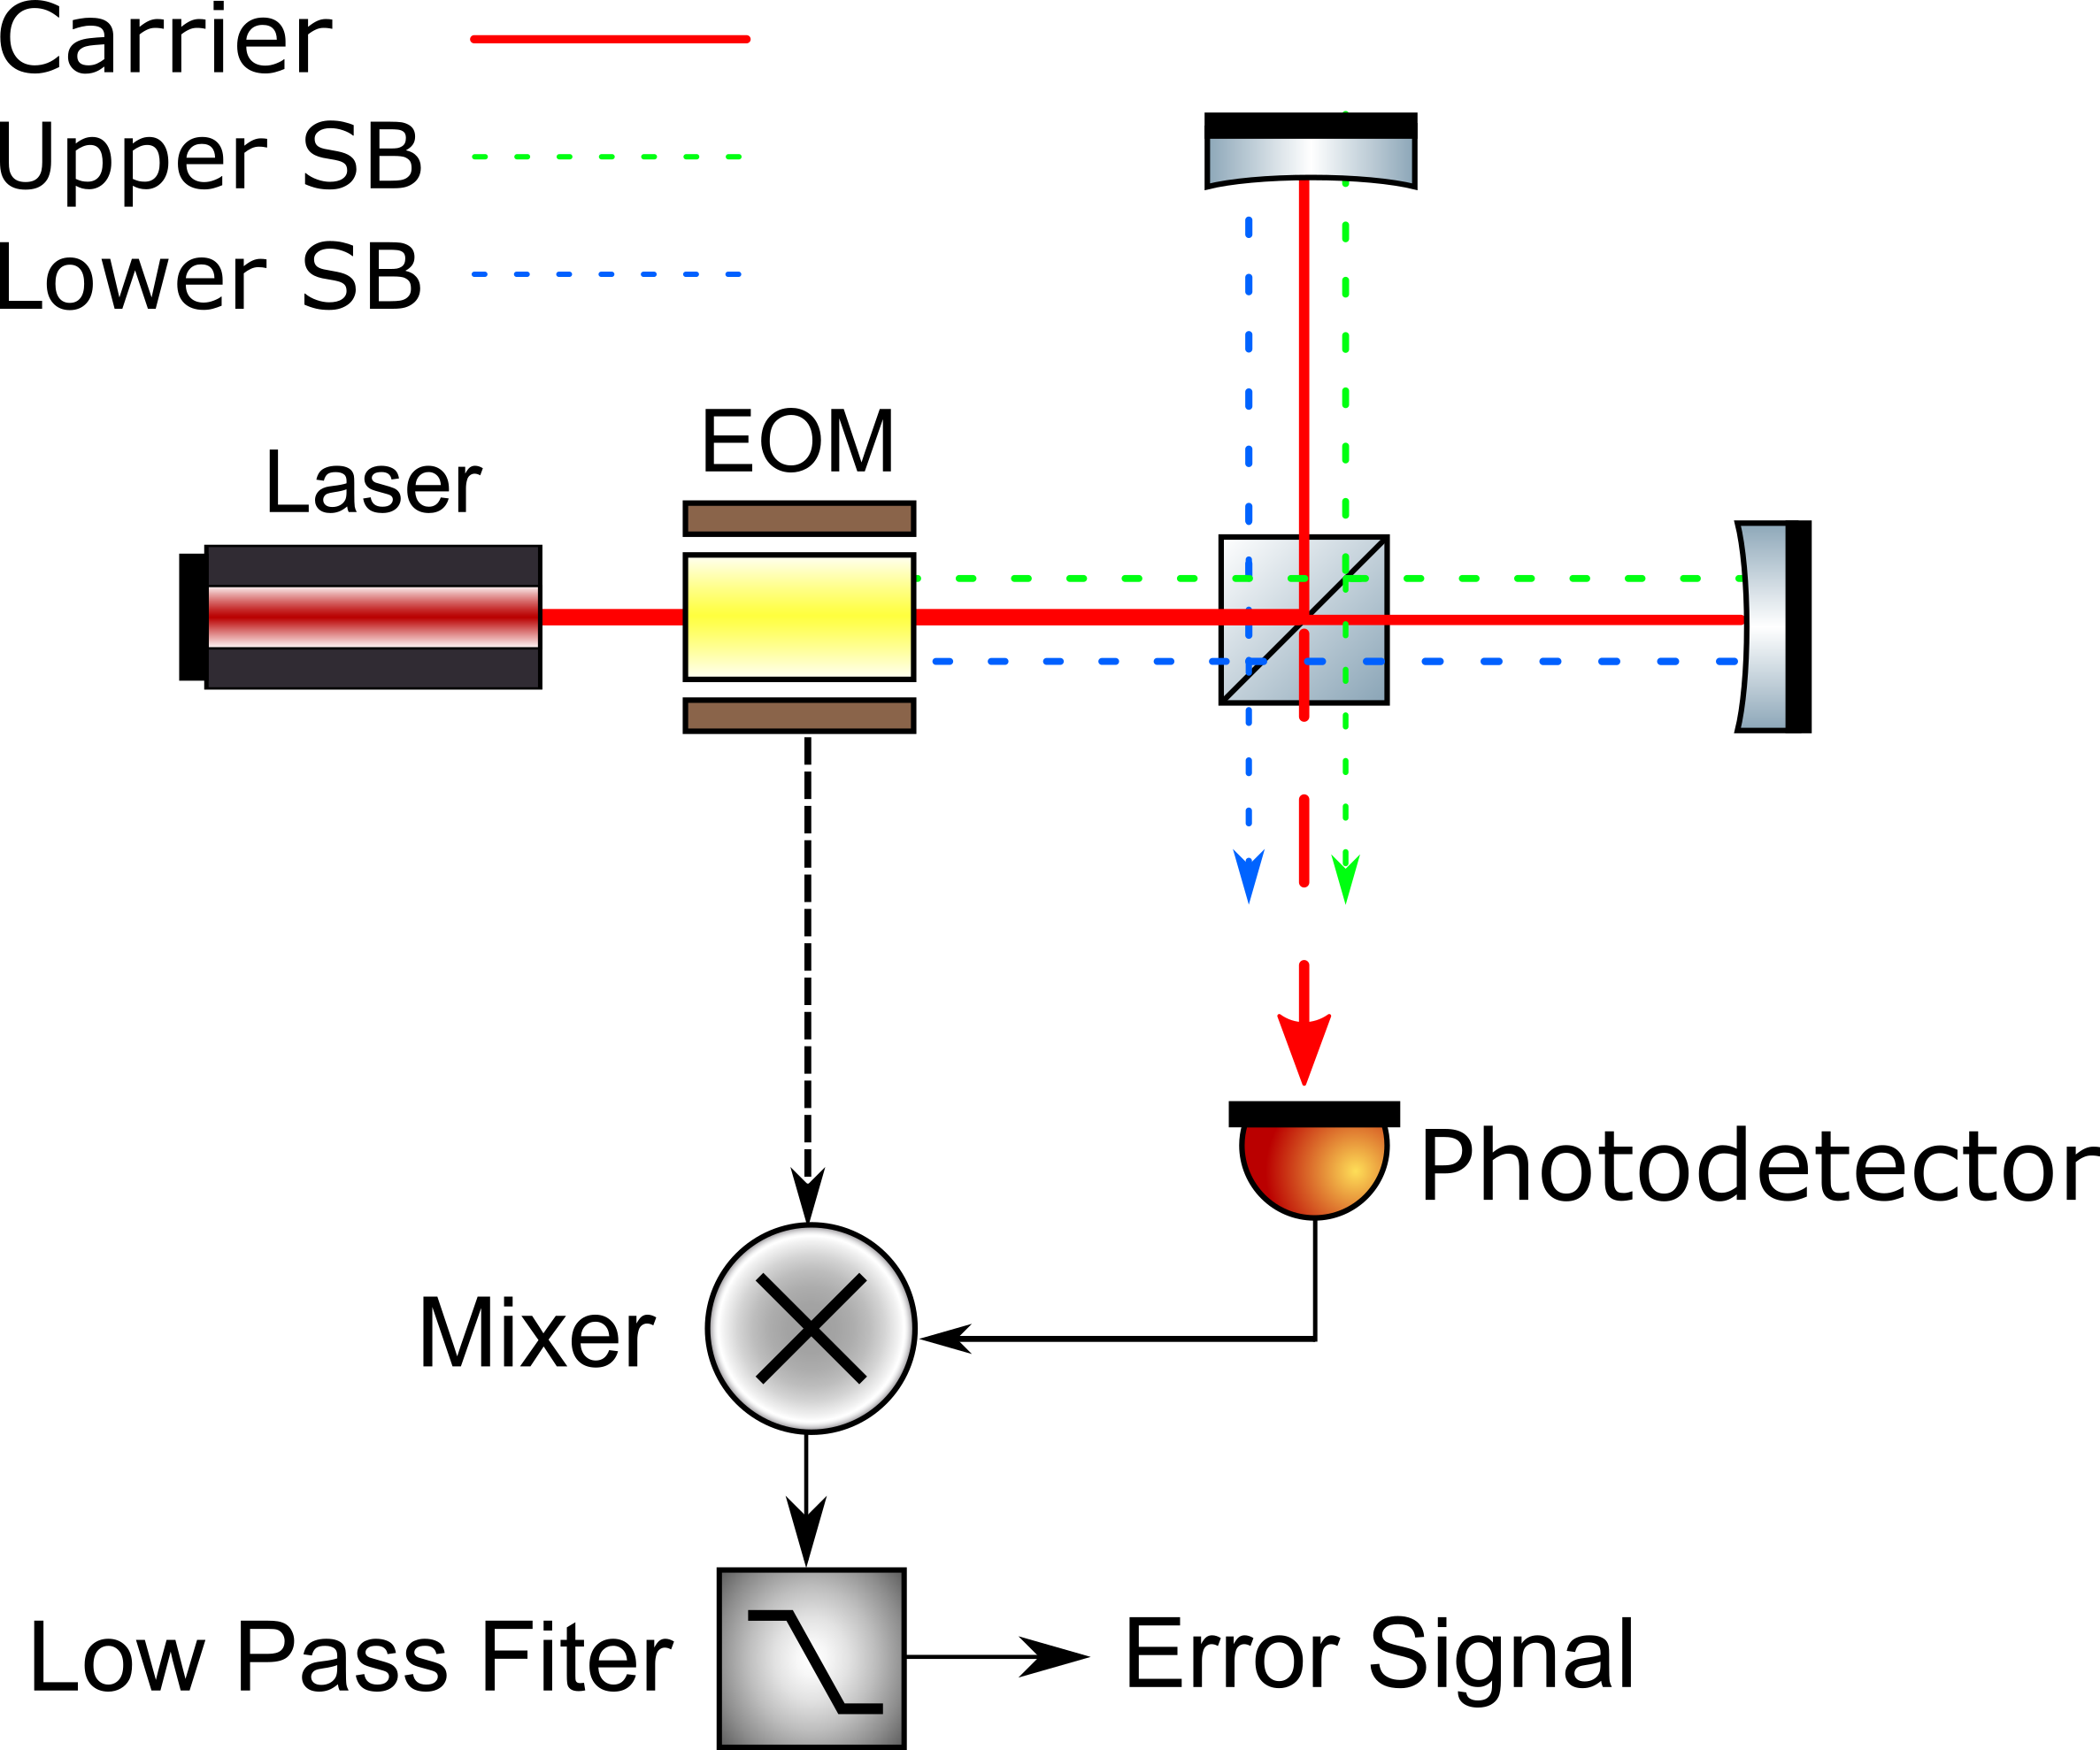
\includegraphics[width=.6 \textwidth]{../Figures/SimpleMichelsonHetero.png}
			\caption[A heterodyne detection scheme for interferometers.]  
			{\textbf{A heterodyne detection scheme for interferometers.} The laser enters an electro-optical modulator which creates three fields described by equation \ref{modE} and read out by a photodetector.  The error signal at the output is then filtered and described by equation \ref{eq:SM_hetero}.}
			\label{fig:MichelsonHetero}
		\end{figure}
		
		The	intensity, which is equal to the electric field squared can be described by
		\begin{equation}\label{RFdet}
		\begin{aligned}
			I	= \vert E_{out} \vert^2  =	&\vert E_{C}\vert^2 + \vert E_{SB+}\vert^2 + \vert E_{SB-}\vert^2 \\
										  	& + 2 \mathbf{Re} \{ \; E_{SB+} E^*_{SB-} e^{2i\Omega t} \; \}\\
										  	& + 2 \mathbf{Re} \{ \; (E_{C} E^*_{SB-} +  E_{SB+} E^*_{C} ) e^{i\Omega t} \; \}
		\end{aligned}
		\end{equation}
		The last term is referred to as the $beat$ $note$ between the carrier signal and the sidebands.  It is possible to extract the term at the modulation frequency using a mixer which is an analog device that outputs the product of two inputs. Usually, the same oscillator that was used to modulate the input beam can be one of the mixer inputs, $\cos(\Omega t)$,  so that the demodulated signal is
		\begin{equation}
		\begin{aligned}
		I_{\text{Demod}} 	&\propto \big[ 4 \pi  J_0(\beta) J_1(\beta) \frac{\ell}{\lambda}  \sin(k_{\Omega} \Delta \ell)  \; h_{+}\big] \big[ \cos(\Omega t)  \sin(\Omega t + \phi_{Demod}) \big] \\
					&\propto \big[ 4 \pi  J_0(\beta) J_1(\beta) \frac{\ell}{\lambda}  \sin(k_{\Omega} \Delta \ell)  \; h_{+}\big] \big[ \sin(\phi_{Demod}) + \sin(2\Omega t + \phi_{Demod}) \big]
		\end{aligned}
		\end{equation}
		where $\phi_{\text{Demod}}$ is the phase that can be set by the user in order to account for extra phase shifts (ie. longer cables). After the mixer, there will be signals at DC, $\Omega$, $2\Omega$ and so on. However, the part that is linear in the gravitational wave amplitude will be at DC so a low-pass filter will allow the final signal to dominate \cite{BlackPDH}:
		\begin{equation}\label{eq:SM_hetero}
		S = 4 \pi  J_0(\beta) J_1(\beta) \frac{\ell}{\lambda}  \sin(k_{\Omega} \Delta \ell) \sin(\phi_{Demod}) \; h_{+}
		\end{equation}
		This shows that a RF detection technique will be linear in GW signal with no large DC offset. Setting the carrier on a null point means $\Delta \ell = \frac{k_{\Omega}}{k} \frac{\pi}{2}$ and allows the designer to optimize the Schnupp asymmetry length to get the best signal for some modulation frequency. This type of readout scheme was used in Enhanced LIGO and is called heterodyne detection, where the sideband fields are produced by an EOM and its efficacy depends on the local oscillator's stability \cite{FritschelReadout}.  
		In contrast, the Advanced LIGO scheme uses a homodyne detection \cite{HildDCReadout} method called "DC-Readout".  Here the oscillator field is produced by slightly offsetting the arms away from the dark fringe and letting a small amount of carrier light through the antisymmetric port.  A gravitational wave will induce sidebands on the carrier and this will allow the same mathematics as above to achieve a linear signal in gravitational wave strain. This method benefits from naturally being co-aligned and mode matched with the signal field.  All techniques follow the same logic of beating the field containing useful information with a reference field to extrapolate a linear signal but the differences come from technical noise such as laser intensity fluctuations and effective quantum noise.
	
		\subsection{Fabry-Perot Cavities}\label{FP}
		There are two ways to improve the LIGO detectors: one is to increase the response from gravitational waves and the other is to decrease the noise contributions. From equation \ref{diffphase}, the gravitational wave signal is proportional to the optical path length that the photon travels, which means the most straightforward method of increasing the sensitivity is to make the arms as long as possible (up to the null point described by equation \ref{gwsinc}).  There are two methods to achieve this: a Herriott delay line or a Fabry-Perot resonator, the differences between each method is shown in Figure \ref{fig:FPvDL}.  At the time of writing this thesis, all modern gravitational wave detectors use the latter method.
		
		\begin{figure}[h]
		\centering
		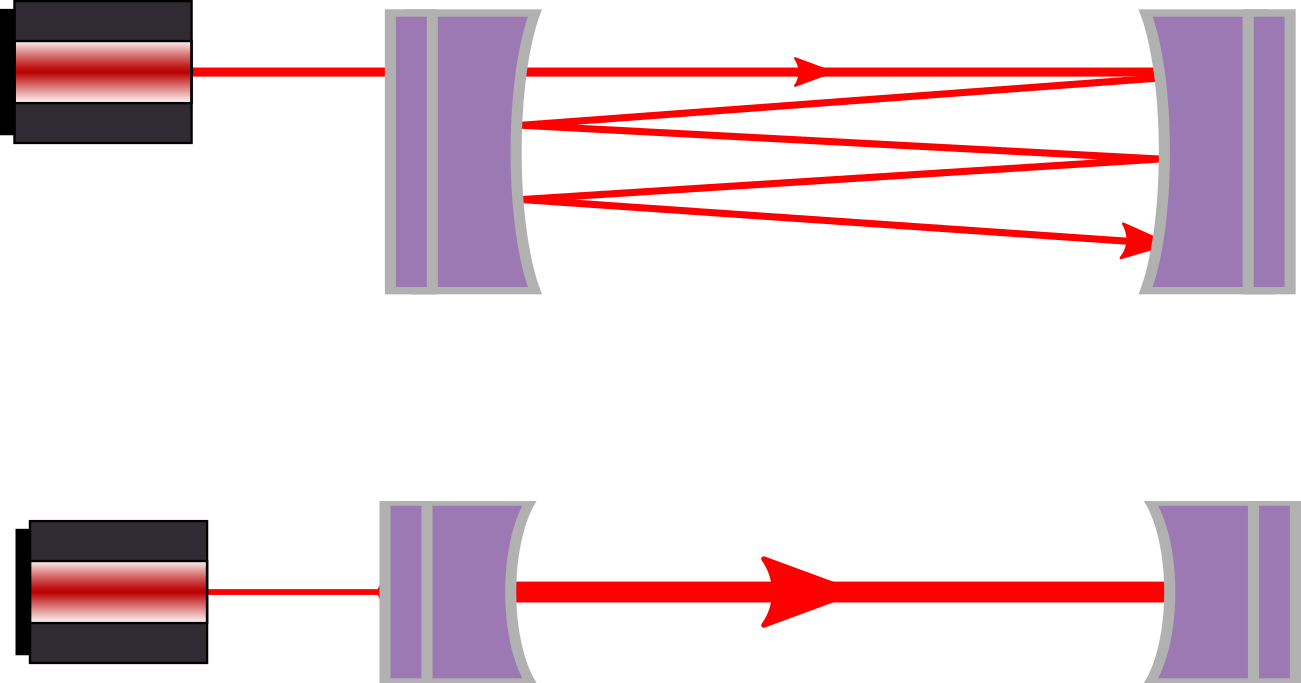
\includegraphics[width=.5 \textwidth]{../Figures/FPvDL.png}
		\caption{Delay Line (top) vs Fabry Perot (bottom)}
		\label{fig:FPvDL}
		\end{figure}
	
		A Fabry-Perot cavity is an optical system comprised of two or more partially transmitting mirrors with one laser input.  To create such a resonator, the user must design a system so that once the electric field has made one round trip within the optical system, the phase of the beam is the same as when it started such that it constructively interferes.  This is done by changing the cavity length, which may seem simple conceptually but in practice, controlling and sensing any optical cavity comes with a few challenges.
		
		To start understanding the longitudinal degree of freedom, consider a two mirror system in Figure [FabryPerotFig] which is separated by a length $L$ with reflection and transmission coefficients: $r_1$, $t_1$, $r_2$, $t_2$.  Starting with a plane wave at the input mirror with amplitude $E_0$, the beam will enter the cavity and propagate back between the two mirrors.  The reflected, transmitted, and circulating fields \cite{Saulson}, which are a result of the geometric series, can be described as
		\begin{equation}\label{r_FP}
		E_{REFL} = r_{FP} E_0 = \bigg(-r_1 + \frac{t_1^2 r_2  e^{-i2kL}}{1-r_1 r_2 e^{-i2kL}} \bigg) E_0
		\end{equation}
		\begin{equation}\label{t_FP}
		E_{TRAN} = t_{FP} E_{0} = \bigg( \frac{t_1 t_2 e^{ikL}}{1-r_1 r_2 e^{-i2kL}}\bigg) E_0
		\end{equation}
		\begin{equation}\label{c_FP}
		E_{CIRC} = c_{FP} E_0 = \bigg(\frac{t_1}{1- r_1 r_2 e^{-2ikL}} \bigg) E_0
		\end{equation}
		The fields above are all highly dependent on the round trip phase and become resonant when the cavity length is $L = n \lambda / 2$ and the circulating coefficient in the cavity is maximized such that the gain is
		\begin{equation}
		\text{Gain} = c^2_{FP} \vert_{\text{resonating}} = \bigg( \frac{t_1}{1-r_1 r_2}\bigg)^2
		\end{equation}
		Depending on the relative reflection coefficients of the input and output mirrors, the fields on resonance will be different in amplitude.  If the input reflection  Figure[UnderOverCritCoupled].
		
		\begin{figure}[ht]
			\centering
			\begin{subfigure}[b]{0.45\textwidth}
				\centering
				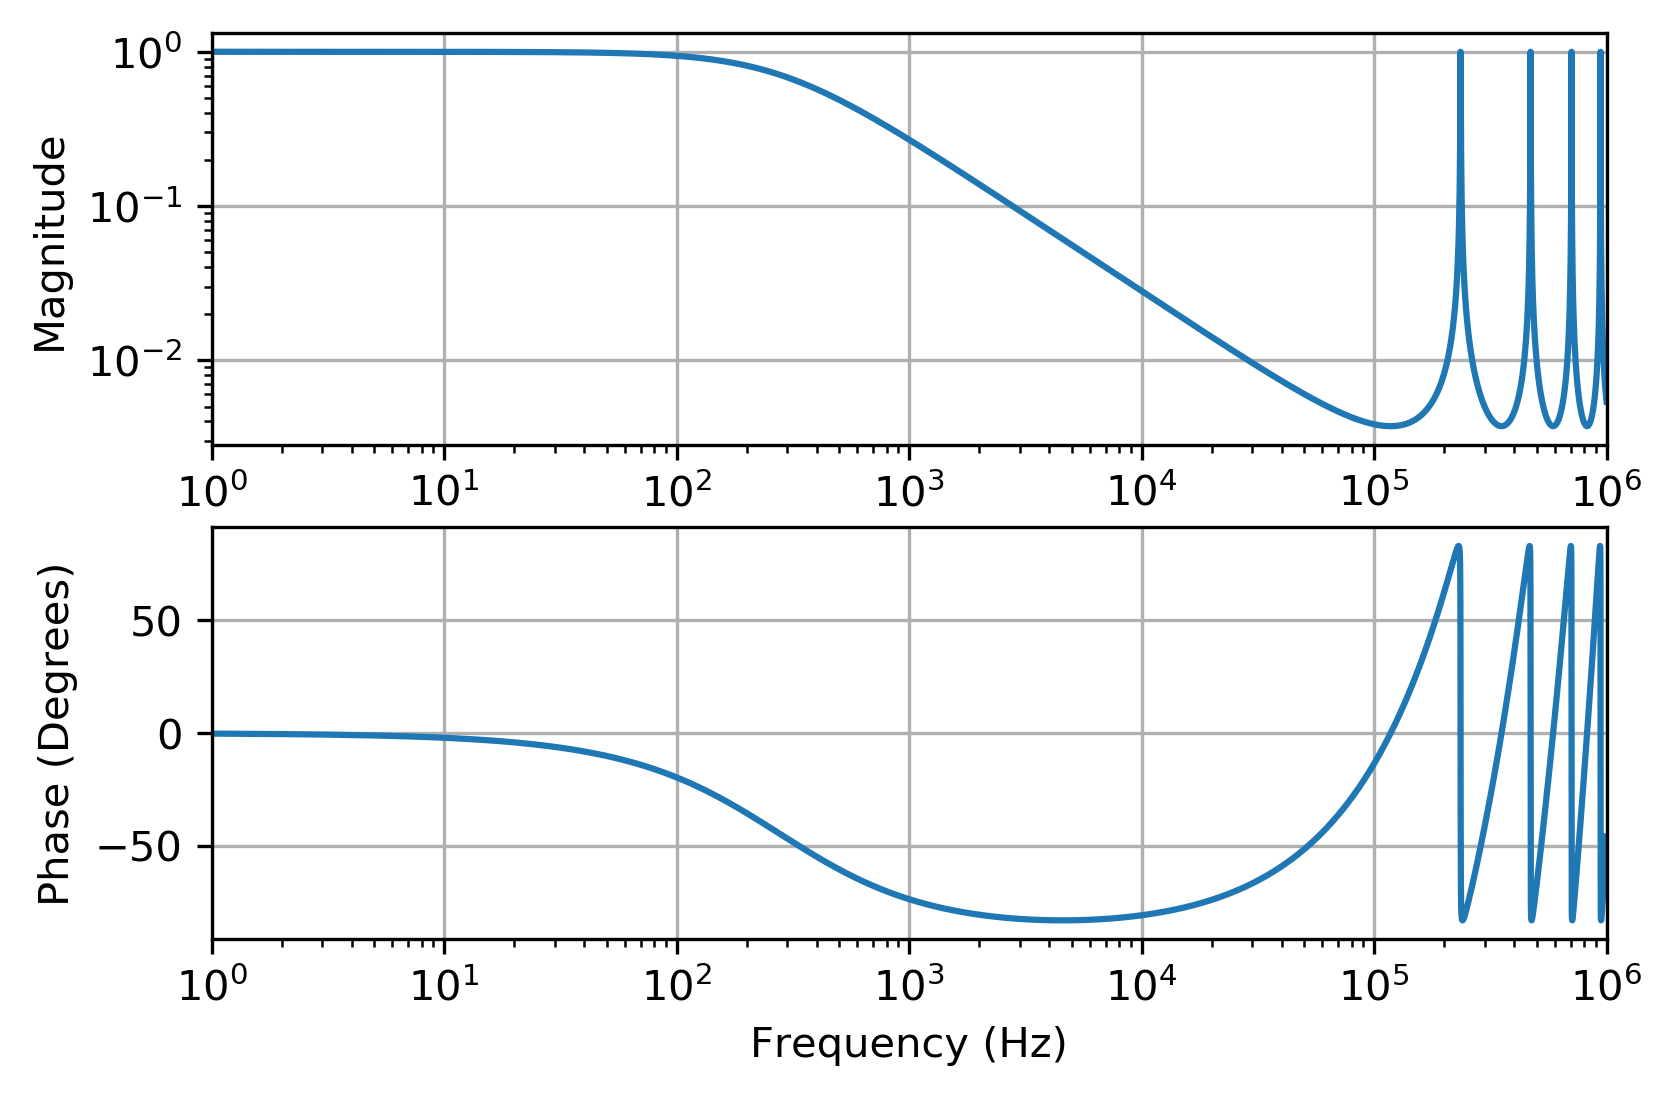
\includegraphics[width=\textwidth]{../Figures/FP_L_TF.png}
				\caption{Transfer function with respect to L}
				\label{fig:FP_L}
			\end{subfigure}
			\hfill
			\begin{subfigure}[b]{0.45\textwidth}
				\centering
				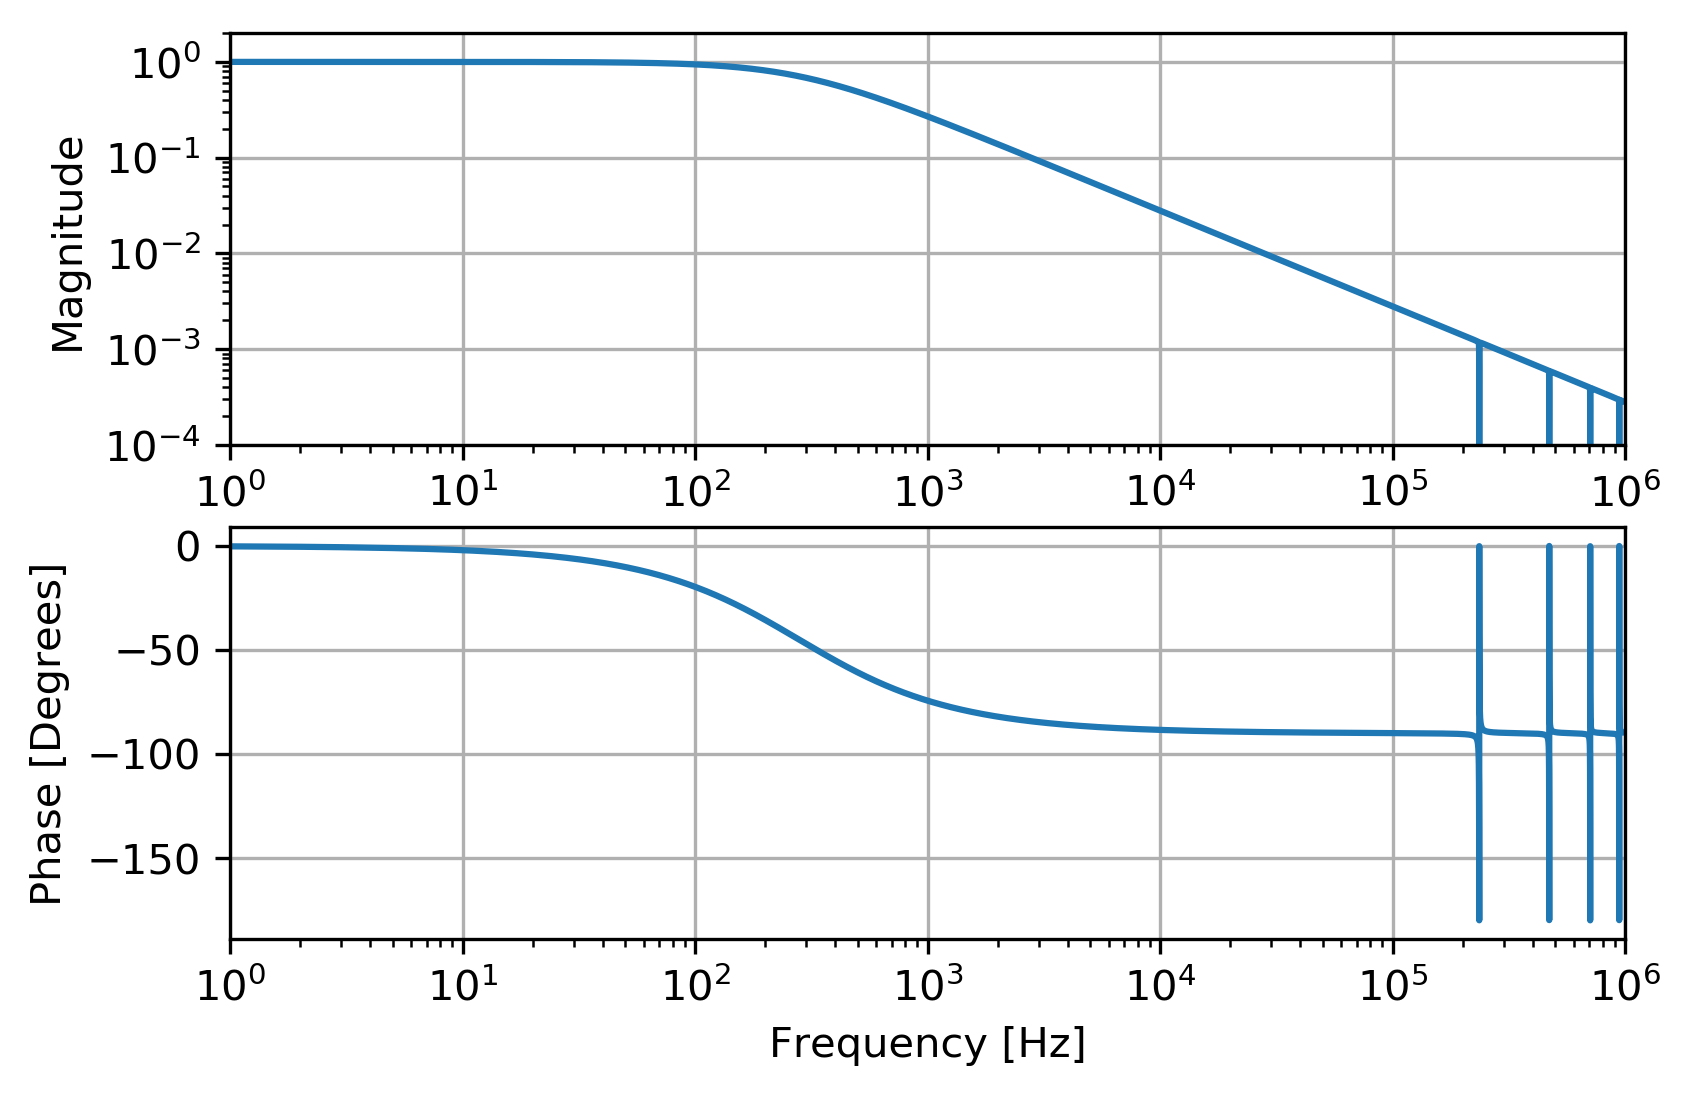
\includegraphics[width=\textwidth]{../Figures/FP_F_TF.png}
				\caption{Transfer function with respect to F}
				\label{fig:FP_F}
			\end{subfigure}
			\caption{Bode Plots of the Fabry Perot response}
			\label{fig:FP_Bode}
		\end{figure}
		
		Notice that the fields are dependent on the cavity length and laser frequency, $2kL$, so one might naively determine that modulating the two parameters independently cause the same effect.  However, when both are changing by large amounts, they are related by a frequency dependent transfer function 
		\begin{equation}
		C(s) \frac{\Delta w}{w} = -\frac{\Delta L}{L}
		\end{equation}
		where $C(s) = \frac{1-e^{-2sL/c}}{2sL/c}$ in the Laplace domain Figure[FreqRespFP]. Only when the cavity is on or near resonance, then the frequency and length variations are related by $\frac{\Delta w}{w} = -\frac{\Delta L}{L}$.
		
	
			\begin{figure}[ht]
		\centering
		\begin{subfigure}[b]{0.45\textwidth}
			\centering
			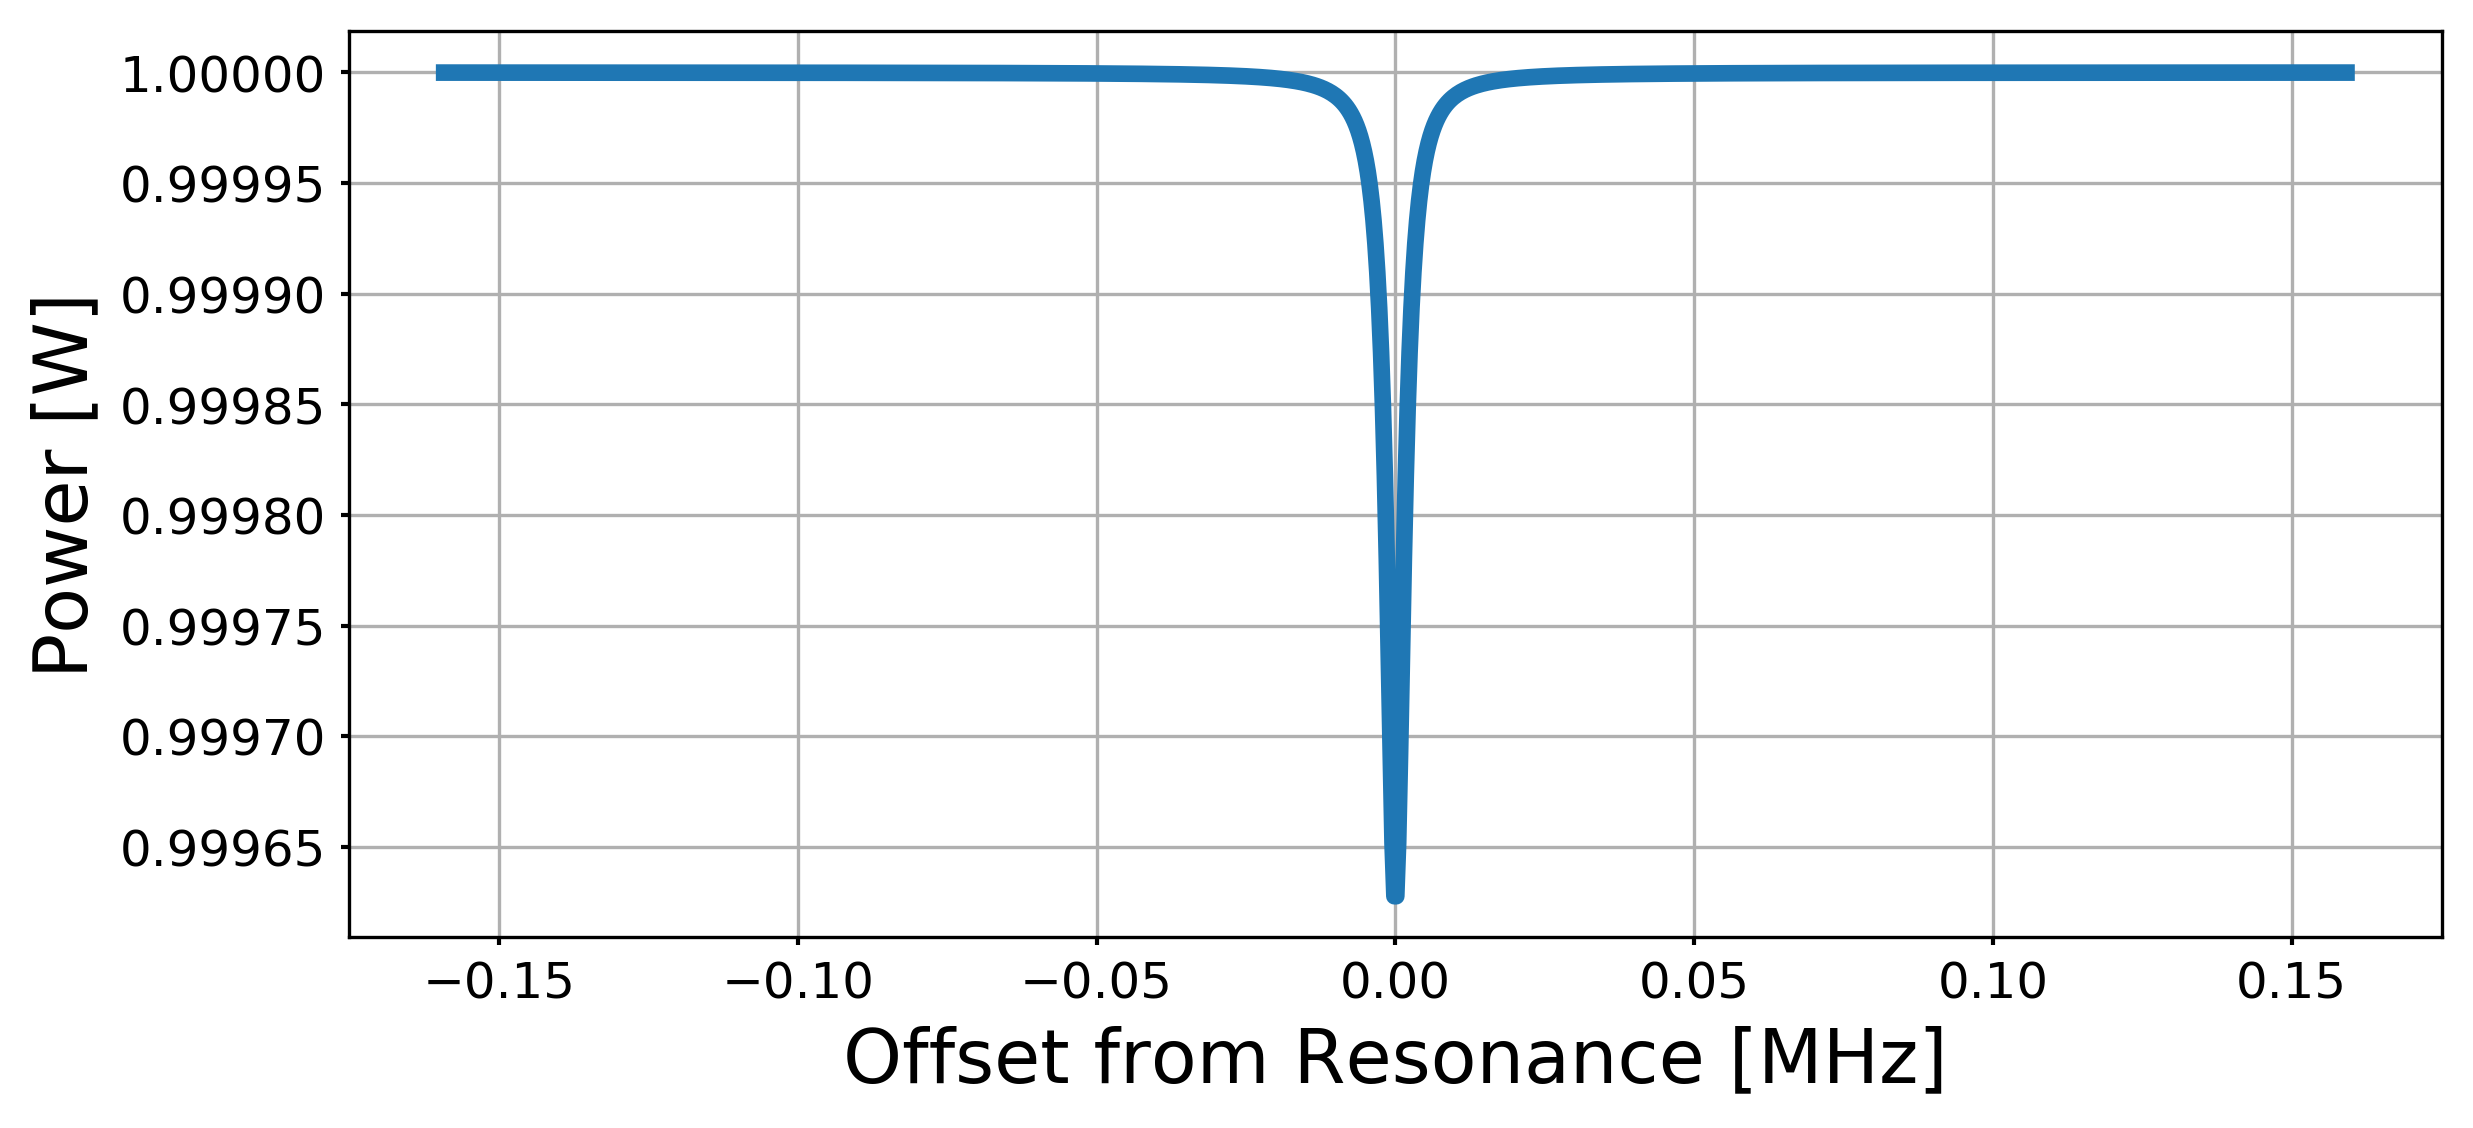
\includegraphics[width=\textwidth]{../Figures/Arm_Refl.png}
			\caption{Reflected Power}
			\label{fig:FP_refl}
		\end{subfigure}
		\hfill
		\begin{subfigure}[b]{0.45\textwidth}
			\centering
			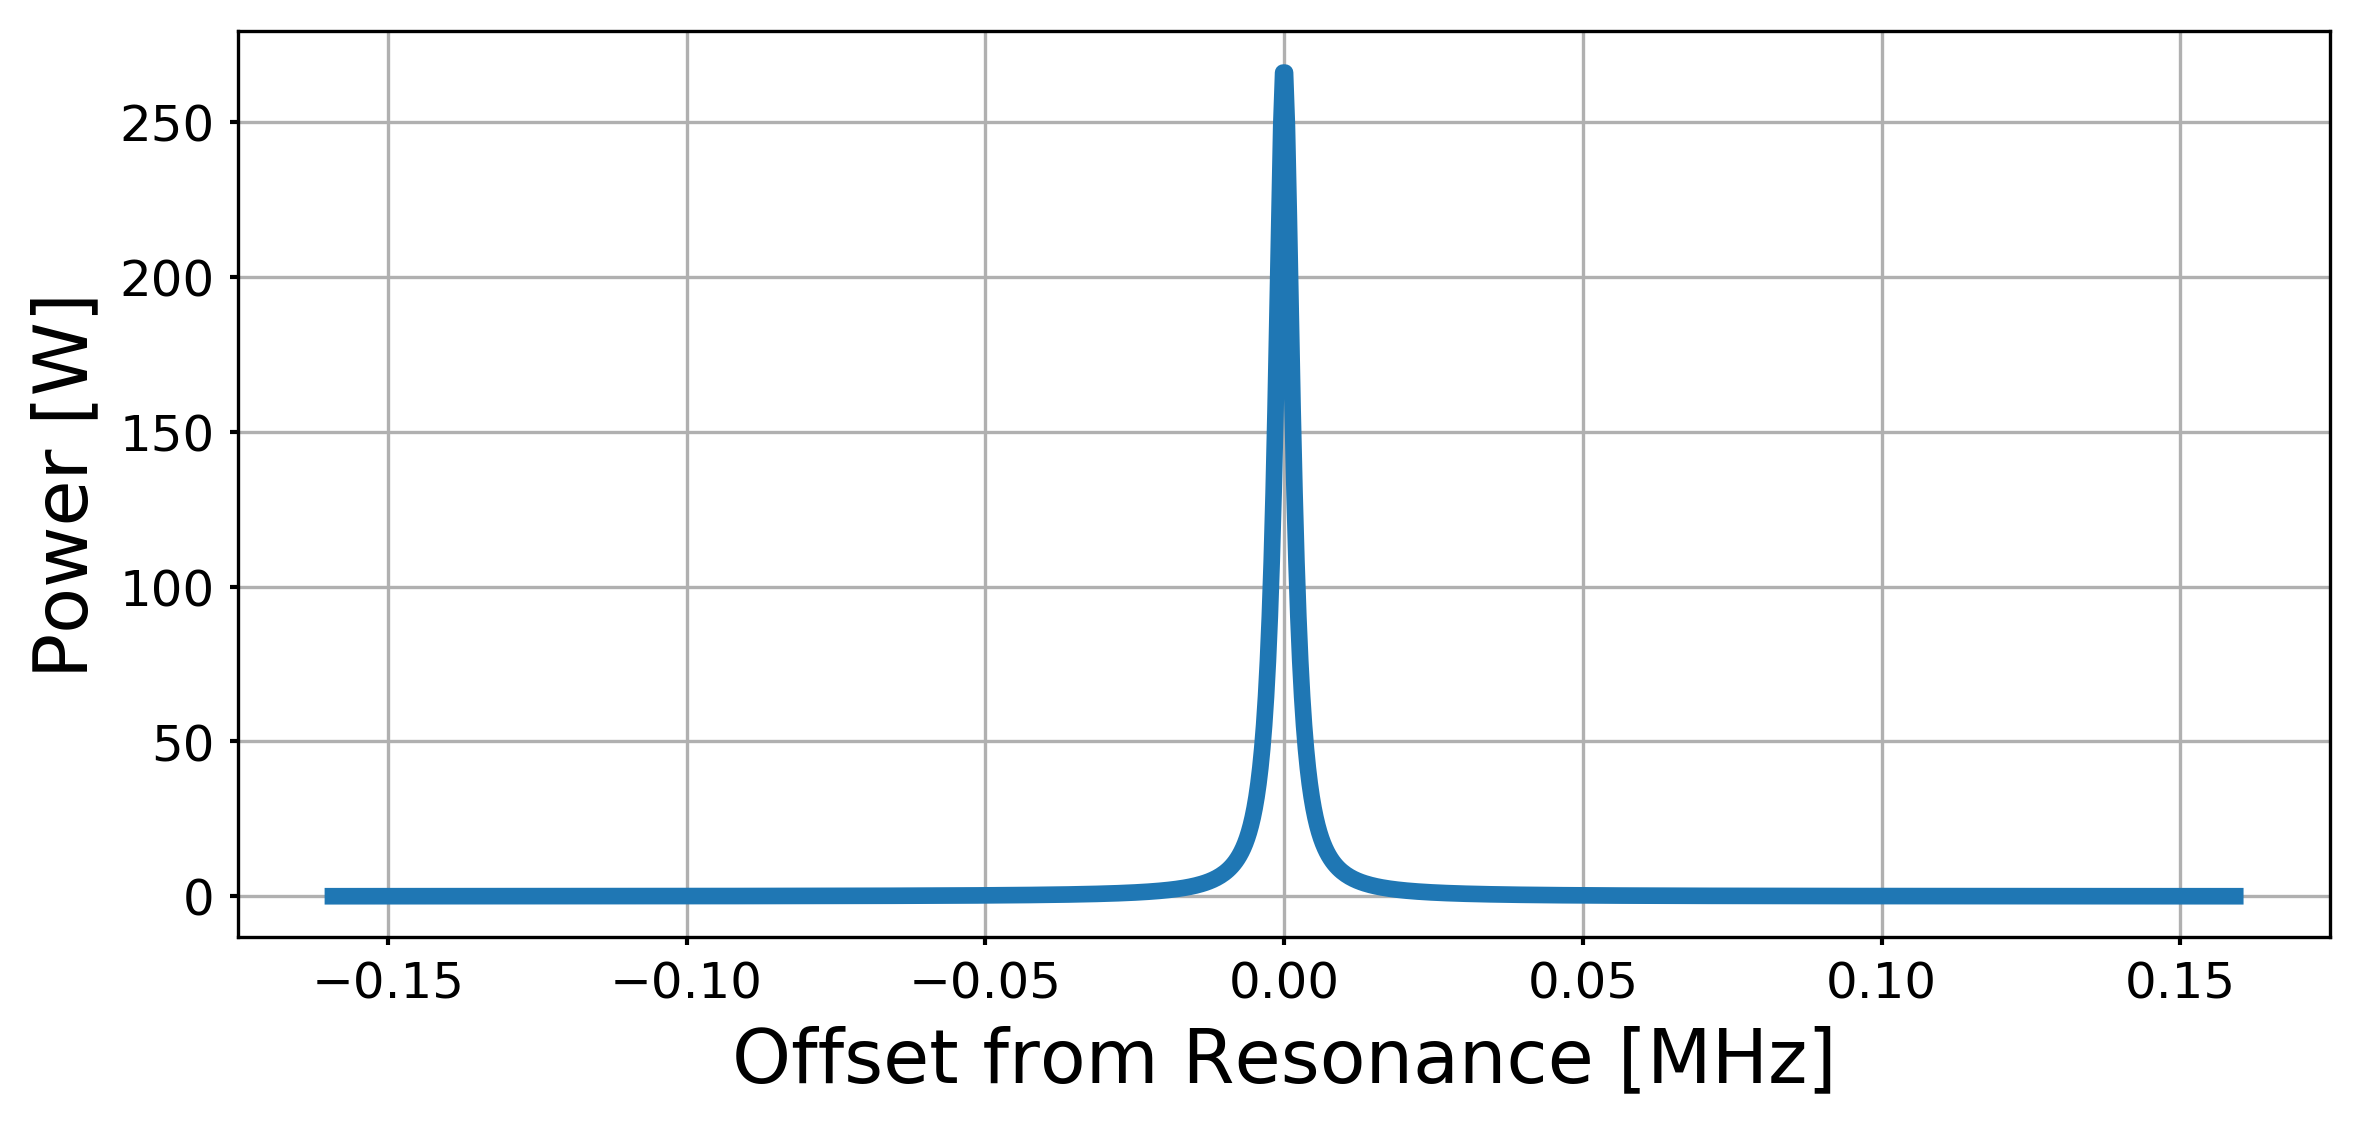
\includegraphics[width=\textwidth]{../Figures/Arm_Circ.png}
			\caption{Circulating Power}
			\label{fig:FP_circ}
		\end{subfigure}
		\hfill
		\begin{subfigure}[b]{0.45\textwidth}
			\centering
			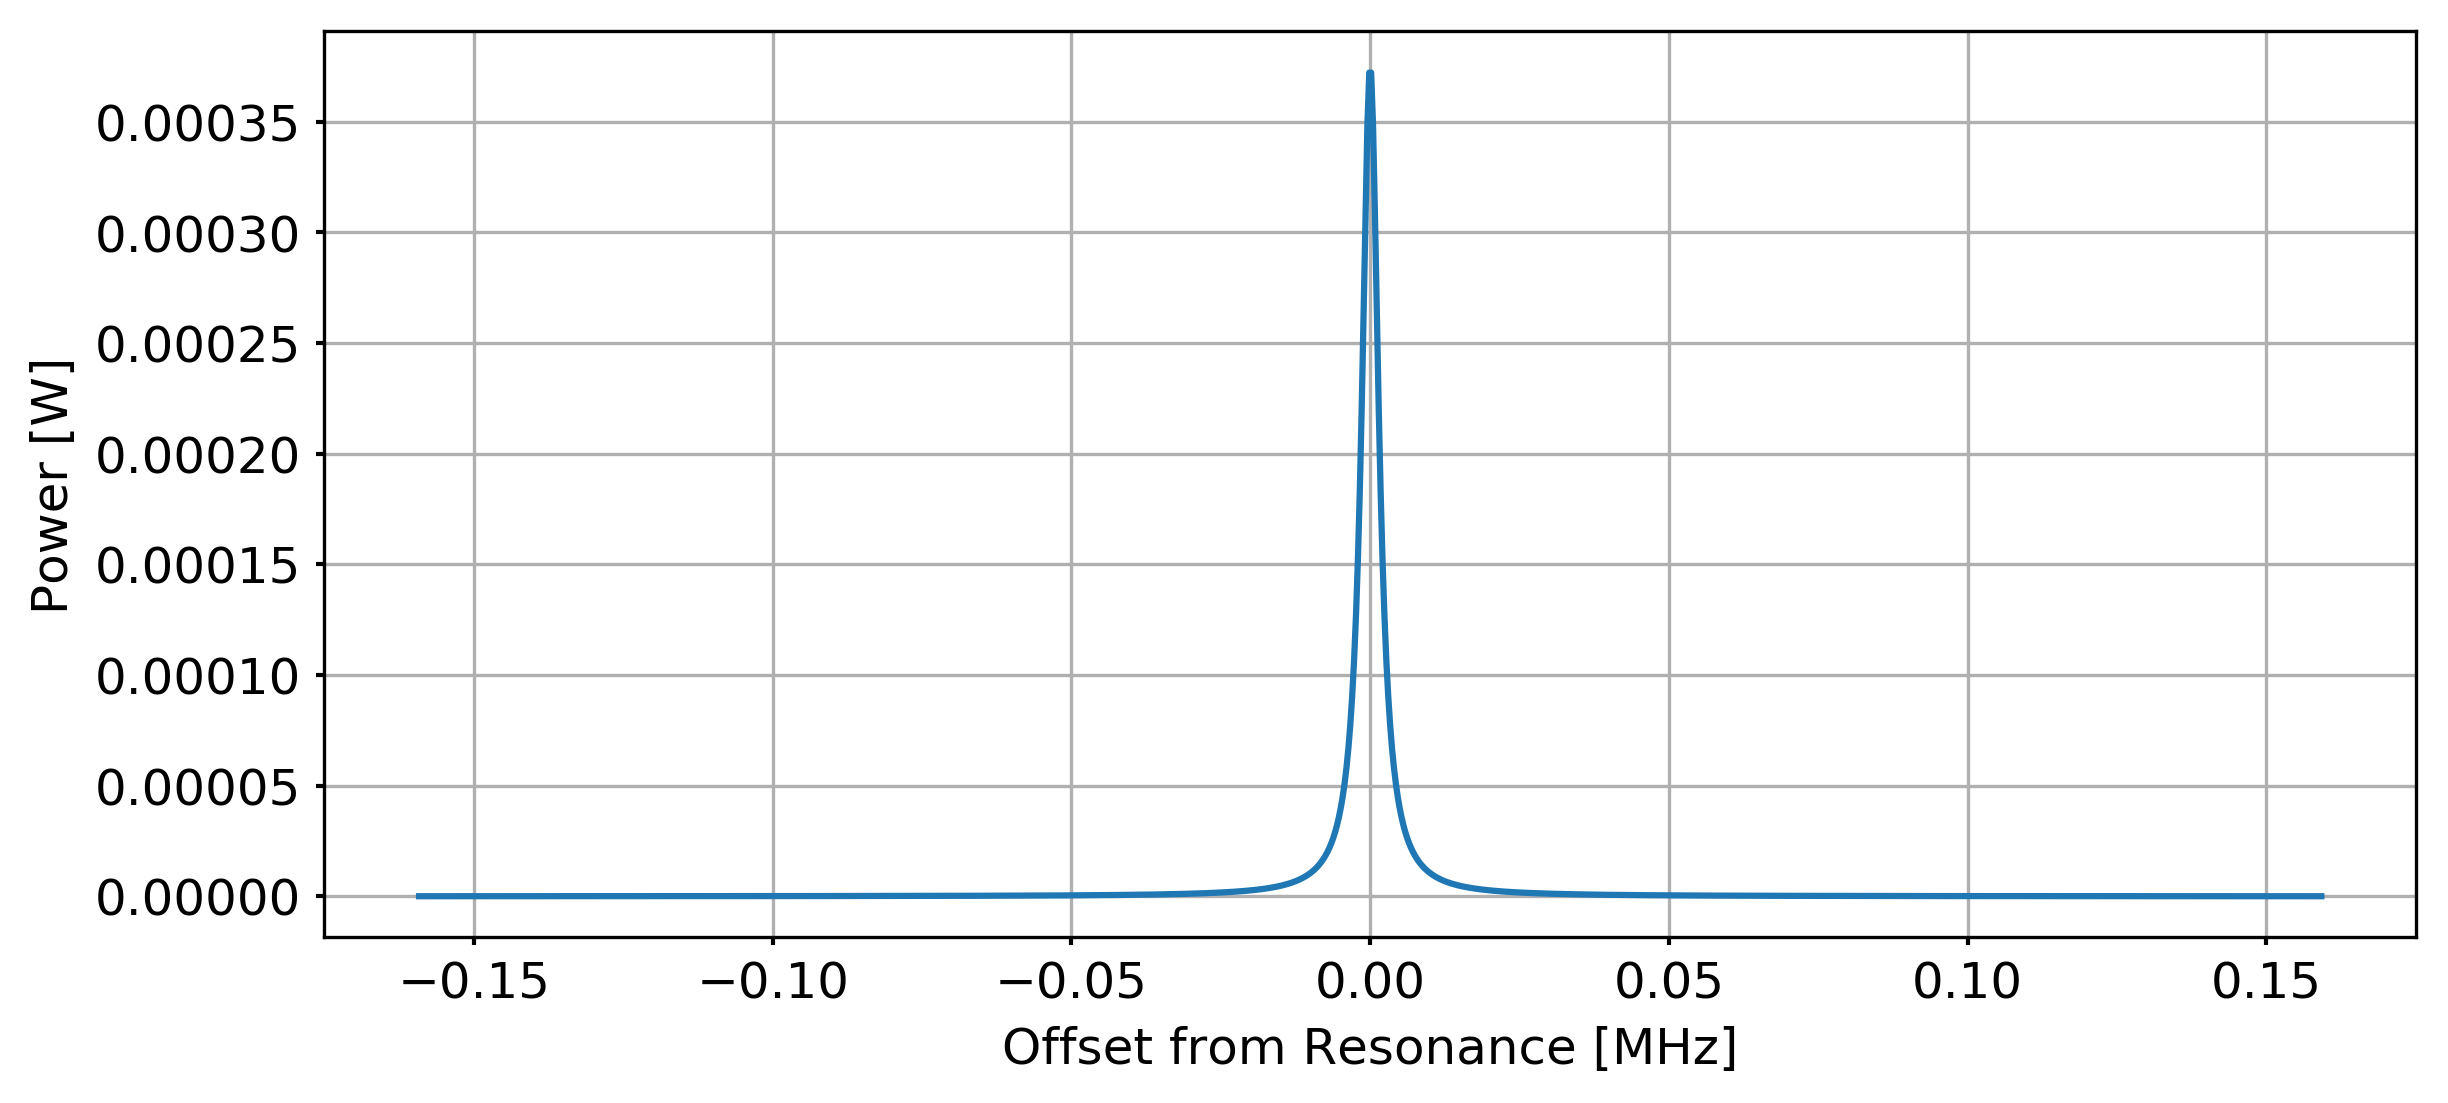
\includegraphics[width=\textwidth]{../Figures/Arm_Tran.png}
			\caption{Transmitted Power}
			\label{fig:FP_tran}
		\end{subfigure}
		\caption[The reflected, circulating, and transmitted powers for a single Fabry-Perot cavity.]
		{The  has properties in Table [] to represent one of the LIGO 4km arms which are highly over-coupled cavities so almost all of the light reflects toward the beamsplitter.  The input power is normalized to 1 Watt to show the relative gain of the circulating power.}
		\label{fig:FP_pwrs}
		\end{figure}
		
		While sweeping through either laser frequency or cavity length and measuring the reflected (or transmitted) fields, there are features of the power spectrum which relate directly to the cavity's physical properties:
		
		Finesse, or the line width of the resonant peak, function of $r_1$ and $r_2$:
		\begin{equation}\label{finesse}
		\mathbb{F} = \frac{\pi \sqrt{r_1 r_2}}{1- r_1 r_2}
		\end{equation}
		Storage Time :
		\begin{equation}
		\tau_{s} = \frac{L}{c \pi} \, \mathbb{F}
		\end{equation}
		Cavity Pole:
		\begin{equation}
		f_{pole} = \frac{1}{4\pi \tau_{s}}
		\end{equation}
		Free Spectral Range:
		\begin{equation}
		f_{FSR}  = \frac{c}{2L}
		\end{equation}

		Stability: In order to prove that an optical cavity is stable, it is useful to introduce the matrices that describe a periodic optical system which is explicitly derived in appendix \ref{FPappendix}.  A Fabry Perot cavity that is separated by distance $L$ with spherical mirrors that have radii of curvature $R_1$ and $R_2$ will need to satisfy 
		\begin{equation}\label{gfactor}
		0 \geq \bigg(1+\frac{L}{R_1}\bigg) \bigg(1+\frac{L}{R_2}\bigg) \geq 1
		\end{equation}
		in order to be geometrically stable (see Figure[BeamGeometryFP]).
		
		Power circulating as a function of our defined parameters slightly off resonance by a length of $\delta L$:
		\begin{equation}
		P_{cav} = \vert c_{FP} \vert^2 = \frac{\text{Gain}}{ 1 + \big(\frac{2\mathbb{F}}{\pi} \big)^2 \, \text{sin}^2(k \delta L) }
		\end{equation}
		
		LIGO uses the frequency response of optical cavities for a number of reasons: Firstly, the round trip phase of the gravitational wave is amplified by the finesse (equation \ref{finesse}) of the 4 kilometer arm cavities, therefore increasing the sensitivity.  Secondly, the input and output of the interferometer's Gaussian beam mode can be refined by only allowing the fundamental mode of the laser to resonate (input and output mode cleaners).  Thirdly, Advanced LIGO uses a dual-recycled Michelson interferometer which means the symmetric port has a mirror inserted to resonate the light reflected from the Fabry Perot arms (power recycling) and another mirror shapes the frequency response of the differential cavity pole at the anti-symmetric port (signal recycling).
		\subsubsection{Achieving Resonance in an Optical Cavity}
		Described above are the theoretical constructs of a FP cavity, but the question remains, how does one practically construct a resonant optical cavity?  The answer comes from using a heterodyne sensing scheme similar to the one described in Section \ref{michelson}.  Except the optical system is not a Michelson interferometer but rather a two mirror cavity.  Still, the heterodyne detection method can apply to a number of different geometries such as triangular or bow-tie cavities shown in Figure[DiffResCavs].
		
		Starting with an input laser and EOM (electro-optical modulator) that imparts upper and lower sidebands at a modulation frequency $\Omega$, the user injects three beams into the optical system described in Equation \ref{modE}.  When placing a photodetector on the reflection port, one should see the cavity's effect on each of the three electric fields.
		
		\begin{equation}
		E_{FP,out} = E_{C} + E_{SB+} + E_{SB-} = 
		\begin{pmatrix}
		r_{C} 	&   
		\\ 	r_{SB+} &
		\\ 	r_{SB-} &
		\end{pmatrix}
		\begin{pmatrix}
		E_{C,in} &    E_{SB+,in}    &  E_{SB-,in}     
		\end{pmatrix}
		\end{equation}
		
		where the reflection coefficients follow equation \ref{r_FP}.  Because sidebands are frequency shifted, they will effectively $see$ a different cavity than the carrier and the total phase accumulated between the fields will be different. To make a good reference for the resonant carrier beam, the modulation frequency, $k_{\Omega}$, is chosen such that sidebands are be anti-resonant in the cavity.  
		\begin{equation}
		r_{C} = -r_1 + \frac{t_1^2 r_2  e^{-i2kL}}{1-r_1 r_2 e^{-i2kL}}
		\end{equation}
		and 
		\begin{equation}
		r_{SB\pm} = -r_1 + \frac{t_1^2 r_2  e^{-i2(k+k_{\Omega})L}}{1-r_1 r_2 e^{-i2(k+k_{\Omega})L}}
		\end{equation}
		The formalism to read out the error signal is the shown in Equation \ref{RFdet}. Using a photodetector in reflection (see Figure \ref{fig:FPControl}), the error signal will be linearly proportional to the laser frequency and cavity length \cite{BlackPDH}.
		\begin{equation}
		\text{Error Signal} \propto \frac{L \mathbb{F}}{\lambda} \bigg[\frac{\delta w}{w} + \frac{\delta L}{L}\bigg]
		\end{equation}
		
		\begin{figure}[h]
		\centering
		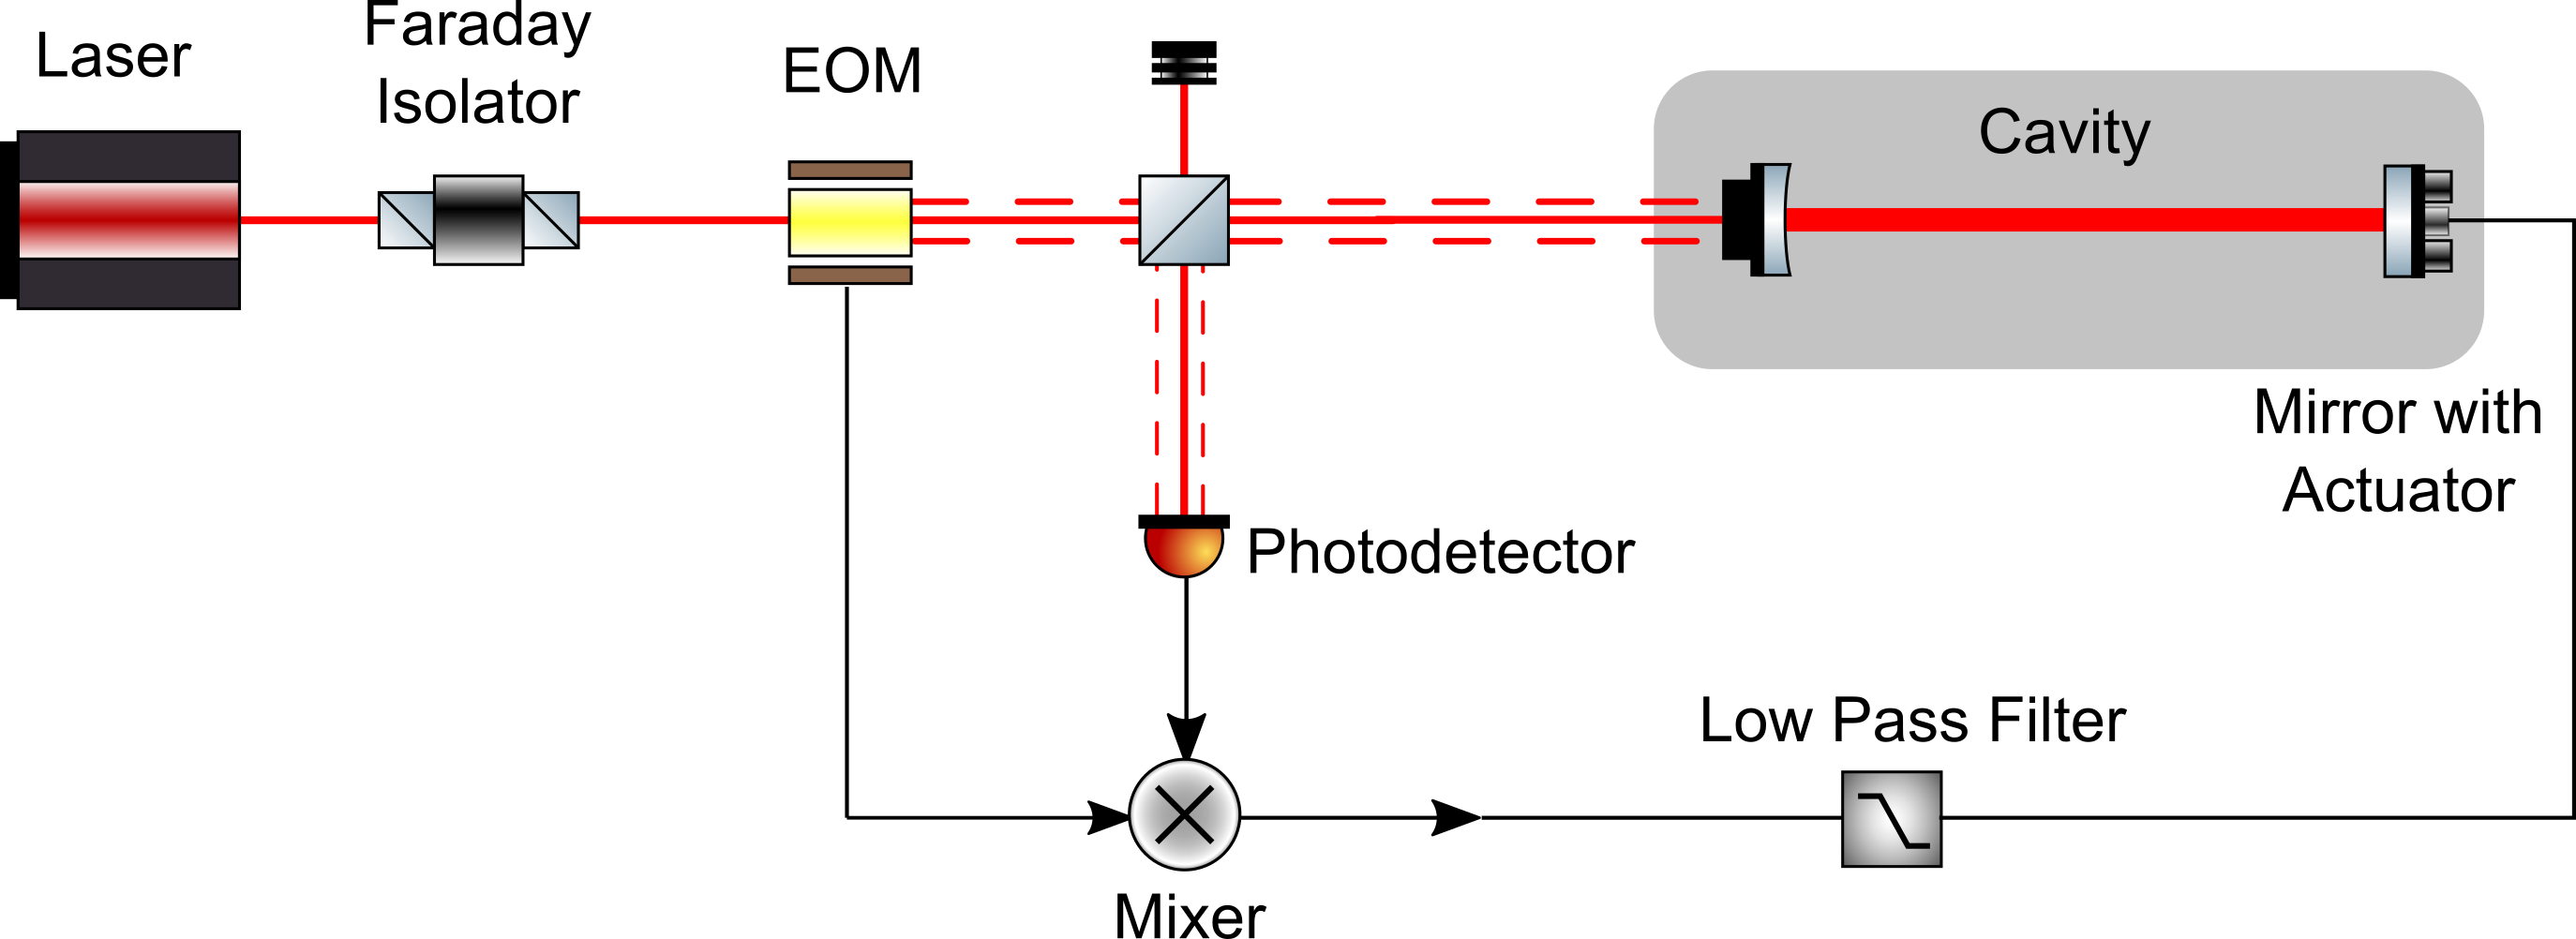
\includegraphics[width=.75 \textwidth]{../Figures/FP_Control.png}
		\caption{Control scheme for an optical cavity.}
		\label{fig:FPControl}
		\end{figure}
	
		\begin{figure}[h]
		\centering
		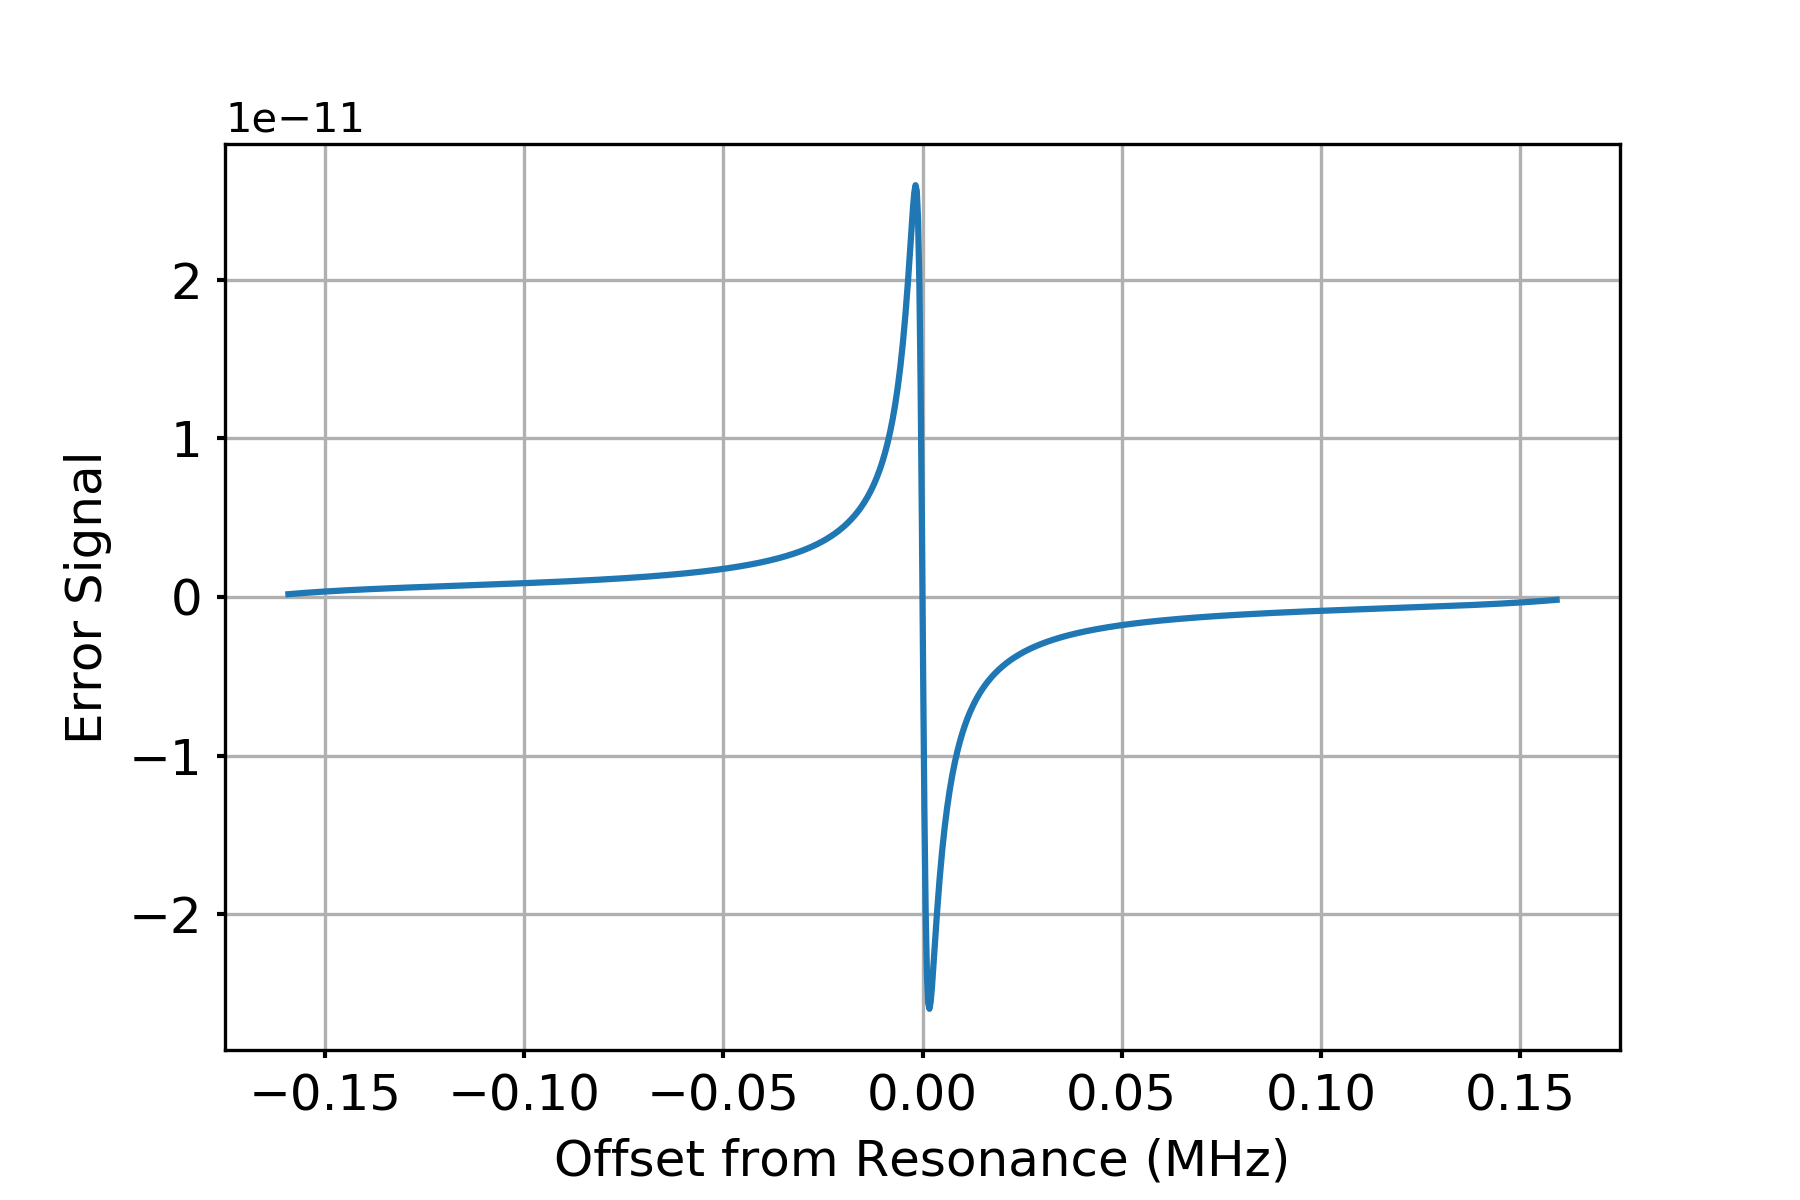
\includegraphics[width=.75 \textwidth]{../Figures/PDH_Err.png}
		\caption[Error signal in reflection]{\textbf{Pound-Drever-Hall (PDH) error signal in reflection of a Fabry Perot cavity.}  By modulating the frequency (or length) close to the zero offset point, the error signal is linear.  However, if the actuation is too far away from the lock point, the signal becomes highly non-linear. }
		\label{fig:FP_err}
		\end{figure}
	
		
		\subsection{Fabry-Perot Michelson}\label{FPmich}
		Using an optical cavity to increase the number of bounces along the 4 kilometer arms will amplify the gravitational wave signal but it will also shape the frequency dependence of the sensitivity as well.  This has already been alluded to in section \ref{measuringGWs} where the overall increase in arm length will tune the response function of equation \ref{gwsinc}.  The same formalism can apply to integrate the use of Fabry-Perot arms into a Michelson interferometer and looking at the signal at the antisymmetric port as a function of gravitational wave frequency. Previously in section \ref{michelson}, it was shown that the RF detection technique required beating the sidebands with a carrier field containing the gravitational wave information.  However, this is not exclusively true because the signal sidebands beating with a reference carrier field could also be a valid way of measuring a signal of interest. In fact, Advanced LIGO employs a homodyne detection called DC readout \cite{FritschelReadout}\cite{FritschelAdvancedLIGO}. The idea is that the carrier field will resonant in the arms but will be slightly modulated due to a gravitational wave.  In effect, the carrier will have audio frequency sidebands imparted on the field shown in Figure[gwsb].  
		
		Figure \ref{fig:FPMichelson} shows an input electric field of $E_0$ incident on a 50/50 beamsplitter which then enters two orthogonal arm cavities of length $L_x$ and $L_y$.  Notice that the distance from the beamsplitter to the input couplers for both arms denoted by $l_x$ and $l_y$ are independent variables, this is to account for the DARM offset which is analogous to the Schnupp asymmetry described in section \ref{michelson}.  After partially transmitting and reflecting at the beamsplitter, the fields will resonate in each of the arm cavities and obey the reflectivity relations described by equation \ref{r_FP}.  Upon recombining at the beamsplitter, the antisymmetric port electric field will be related to the arm fields by,
		\begin{equation}
		E_{\text{AS}} = \frac{1}{\sqrt{2}} [E_{x}^{\text{ARM}} + E_{y}^{\text{ARM}} ] 
		\end{equation}
		where $E_{i}^{\text{ARM}} = E(\omega) \pm [E(+ \omega_{\text{\tiny GW}}) + E(- \omega_{\text{\tiny GW}})] \sin{k\delta l } $ is the reflectionfig:FPMichelson coefficient for the x and y arms which contain the carrier(first term) and GW signal sidebands(last two terms).  Intuitively, one can deduce that the antisymmetric port will only be sensitive to the differential motion between the arm cavities, which means the gravitational wave sidebands in the x-arm will be out of phase with the y-arm.  Also it is important to note that inserting a DC microscopic length shift, $\delta l = l_x - l_y$ allows for some carrier leakage field to propagate towards the antisymmetric port which creates a static reference to form a beat note with the signal sidebands.  The same effect can be achieved by introducing a static offset between the x and y arms; colloquially, this is referred to as DARM offset.
				
		\begin{figure}[ht]
			\centering
			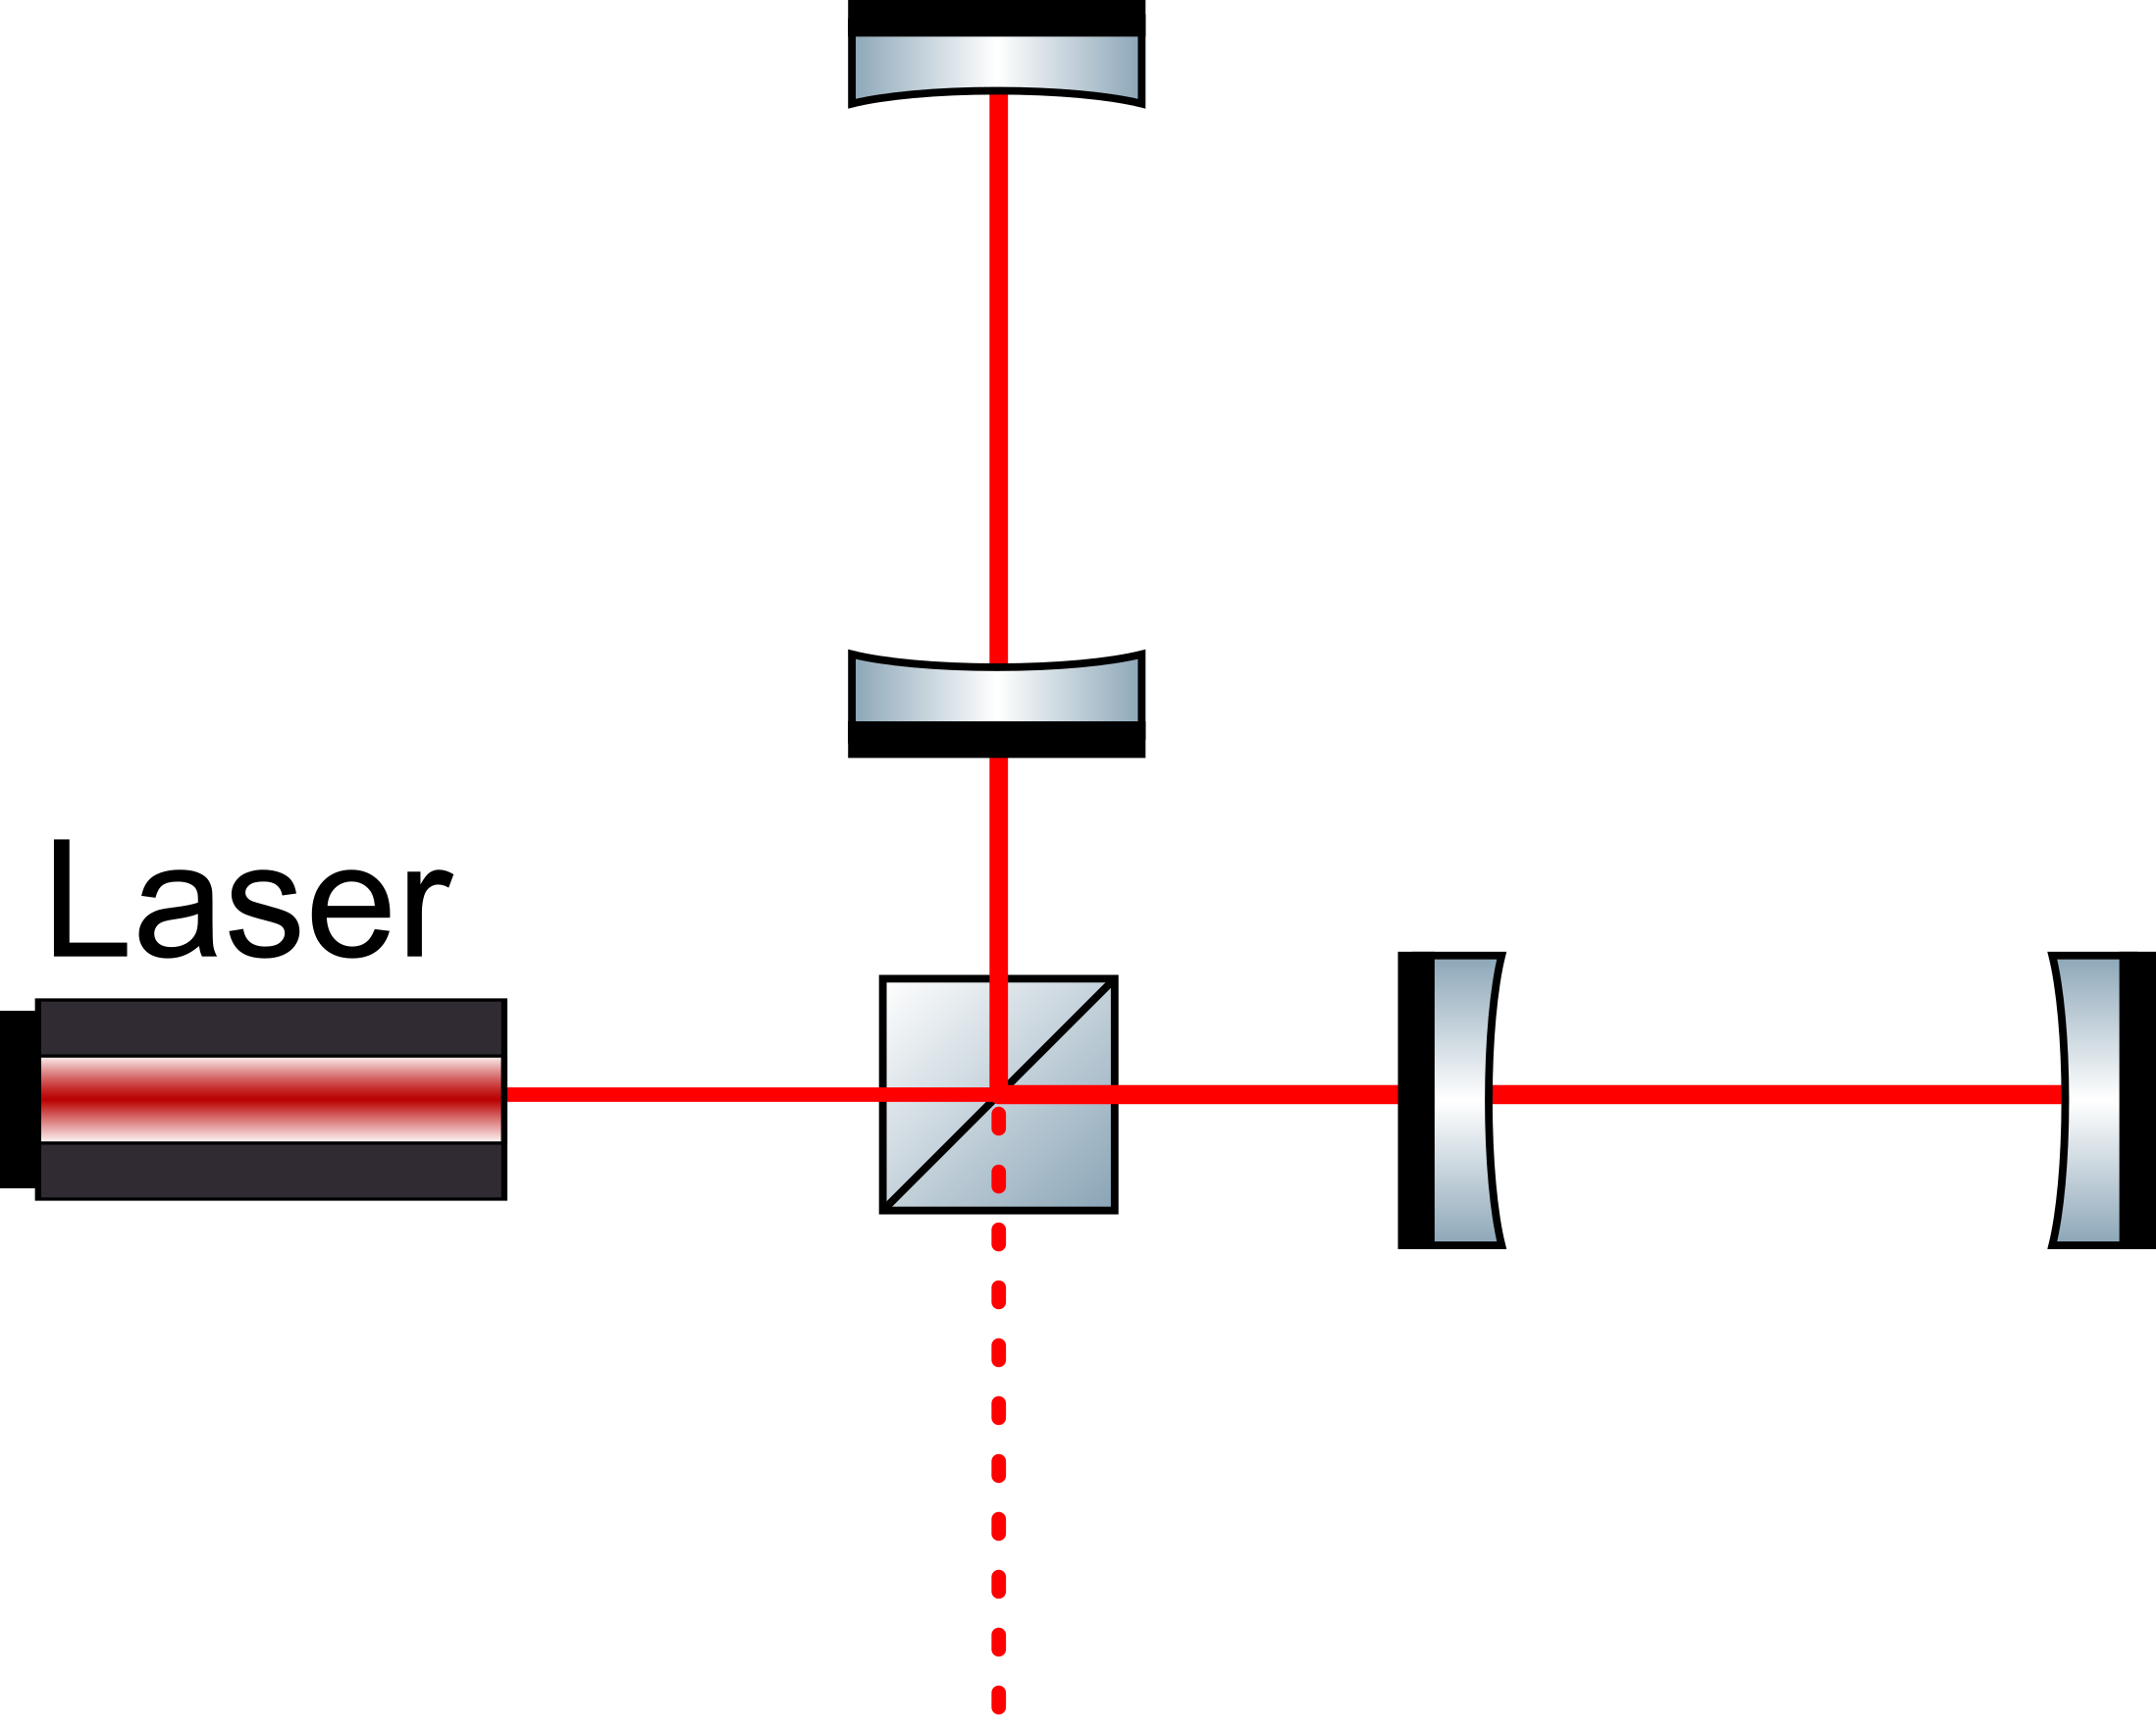
\includegraphics[width=.3 \textwidth]{../Figures/FP_Mich.png}
			\caption{Michelson with Fabry Perot arms}
			\label{fig:FPMichelson}
		\end{figure}
	
		For the carrier field, the amplitude of reflection is simple because the LIGO arms are a strongly overcoupled cavity operating on resonance therefore 
		\begin{equation}
			E(\omega) = \frac{E_0}{\sqrt{2}}  \bigg(-r_1 + \frac{t_1^2 r_2}{1-r_1 r_2} \bigg) \approx -\frac{E_0}{\sqrt{2}}
		\end{equation}
		
		The sidebands are a different story because the modulation caused by the gravitational wave slightly move the field off resonance.  Imagine the carrier circulating in the arms and then suddenly, a disturbance due to a gravitational wave displaces the end mirror at a frequency $\omega_\text{GW}$ by an amount $\Delta L$.   By using the same formalism as the expansion of a modulated field in equation \ref{modE}, the sideband fields can be described by,
		\begin{equation}
		\begin{aligned}\label{Egw}
			E(\pm \omega_{\text{\tiny GW}}) &= \bigg[ \frac{t_1}{1-r_1 r_2 e^{-2ikL}}\bigg] \frac{E_0}{\sqrt{2}} \bigg[\frac{t_1}{1-r_1 r_2 e^{-2i (kL \pm \omega_{\text{\tiny GW}}  \frac{L}{c})}} \bigg] ik\Delta L\\
			& =  \bigg[ \frac{t_1^2}{1-r_1 r_2}\bigg]  \frac{E_0}{\sqrt{2}} \bigg[\frac{ 1}{1-r_1 r_2 e^{-2i  \omega_{\text{\tiny GW}}  \frac{L}{c}}} \bigg] ik\Delta L
		\end{aligned}
		\end{equation}
		The first bracket is the circulating field of the carrier signal amplified by the Fabry Perot cavity and the second bracket is the circulating field slightly off resonance due to the gravitational wave frequency offset.  Setting the fields to resonate already simplifies the equation but it is also reasonable to approximate the gravitational wave as a weak signal and expand the exponential $e^{- 2i \omega_{\text{\tiny GW}}  \frac{L}{c}} \approx 1 - 2i \omega_{\text{\tiny GW}}  \frac{L}{c}$.  This transforms the signal sideband field into a simple form,
		\begin{equation}
		E(\pm \omega_{\text{\tiny GW}}) \approx \bigg[\frac{t_1}{1-r_1r_2}\bigg]^2 \, \frac{E_0}{\sqrt{2}} \, \bigg[\frac{1}{1 \pm i \frac{\omega_{\text{\tiny GW}}}{\omega_p}}\bigg] ik\Delta L
		\end{equation}
		where $\omega_p = \frac{1-r_1r_2}{r_1r_2}\frac{c}{2L}$ is the differential pole frequency; notice that it matches the single arm cavity pole.
		
		The photodiode signal at the antisymmetric port is proportional to the beat note between the carrier and signal sideband that is demodulated in the audio band with a phase $\phi_{D}$,
		\begin{equation}
		\begin{aligned}
			S &\propto 2 [E(\omega) E^*(+\omega_{\text{\tiny GW}}) +  E(-\omega_{\text{\tiny GW}}) E^*(\omega) ] \sin{(k\delta l)} \sin{(\phi_{D})} \\
			  &\propto E_0^2 \; \frac{8\pi L}{\lambda}  \bigg[\frac{t_1}{1-r_1r_2}\bigg]^2 \bigg[\frac{1}{1 - i \frac{\omega_{\text{\tiny GW}}}{\omega_p}}\bigg] \sin{(k\delta l)} \sin{(\phi_{D})} h_{\text{\tiny GW}}
		\end{aligned}
		\end{equation}
		where the length disturbance $\Delta L$ was transformed to originate from a gravitational wave signal $k \Delta L = \frac{2\pi L}{\lambda} h_{\text{\tiny GW}}$.
		The response in this particular interferometer setup to the presence of differential length motion is linearly proportional to the gravitational wave amplitude as well as the input power $P_0 = E_0^2$, but there is also a frequency dependent component which is the same as a single Fabry-Perot arm that acts like a low pass filter above the corner frequency.

		\subsection{Power-Recycled Fabry-Perot Interferometers}
		
		\begin{figure}[ht]
			\centering
			\begin{subfigure}[b]{0.3\textwidth}
				\centering
				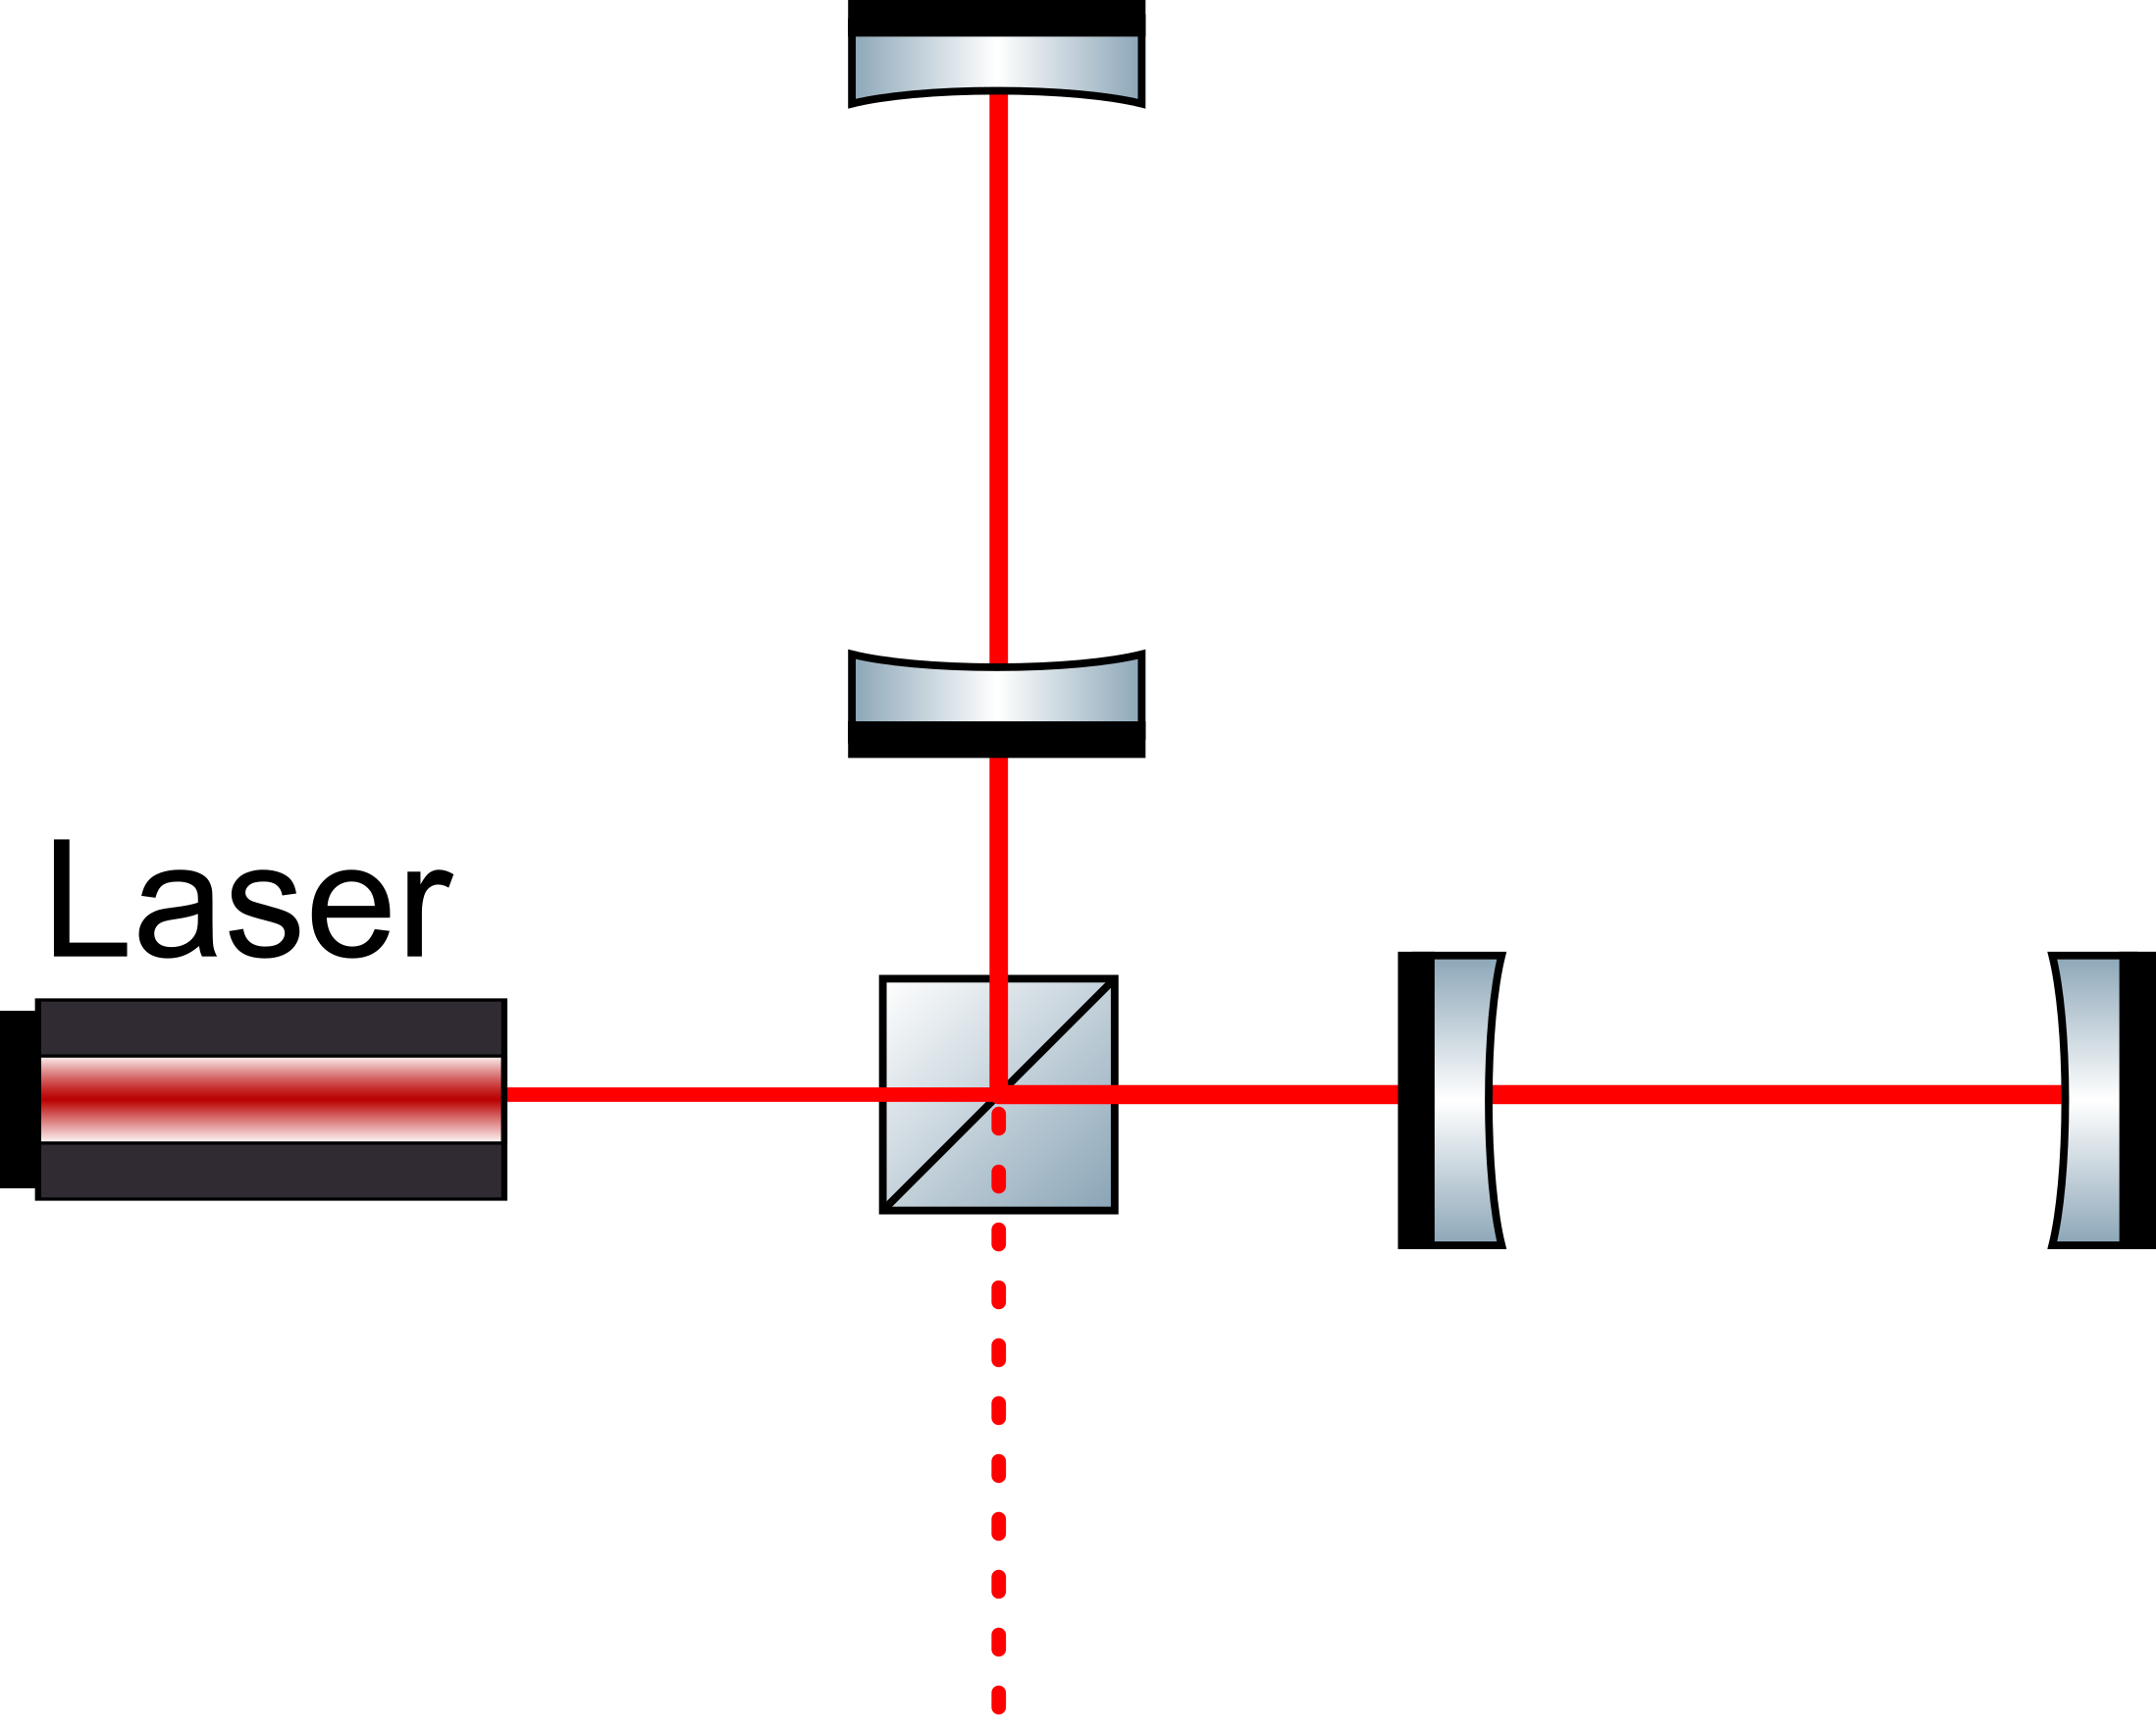
\includegraphics[width=\textwidth]{../Figures/FP_Mich.png}
				\caption{Fabry Perot Michelson}
				\label{fig:FPMich}
			\end{subfigure}
			\hfill
			\begin{subfigure}[b]{0.3\textwidth}
				\centering
				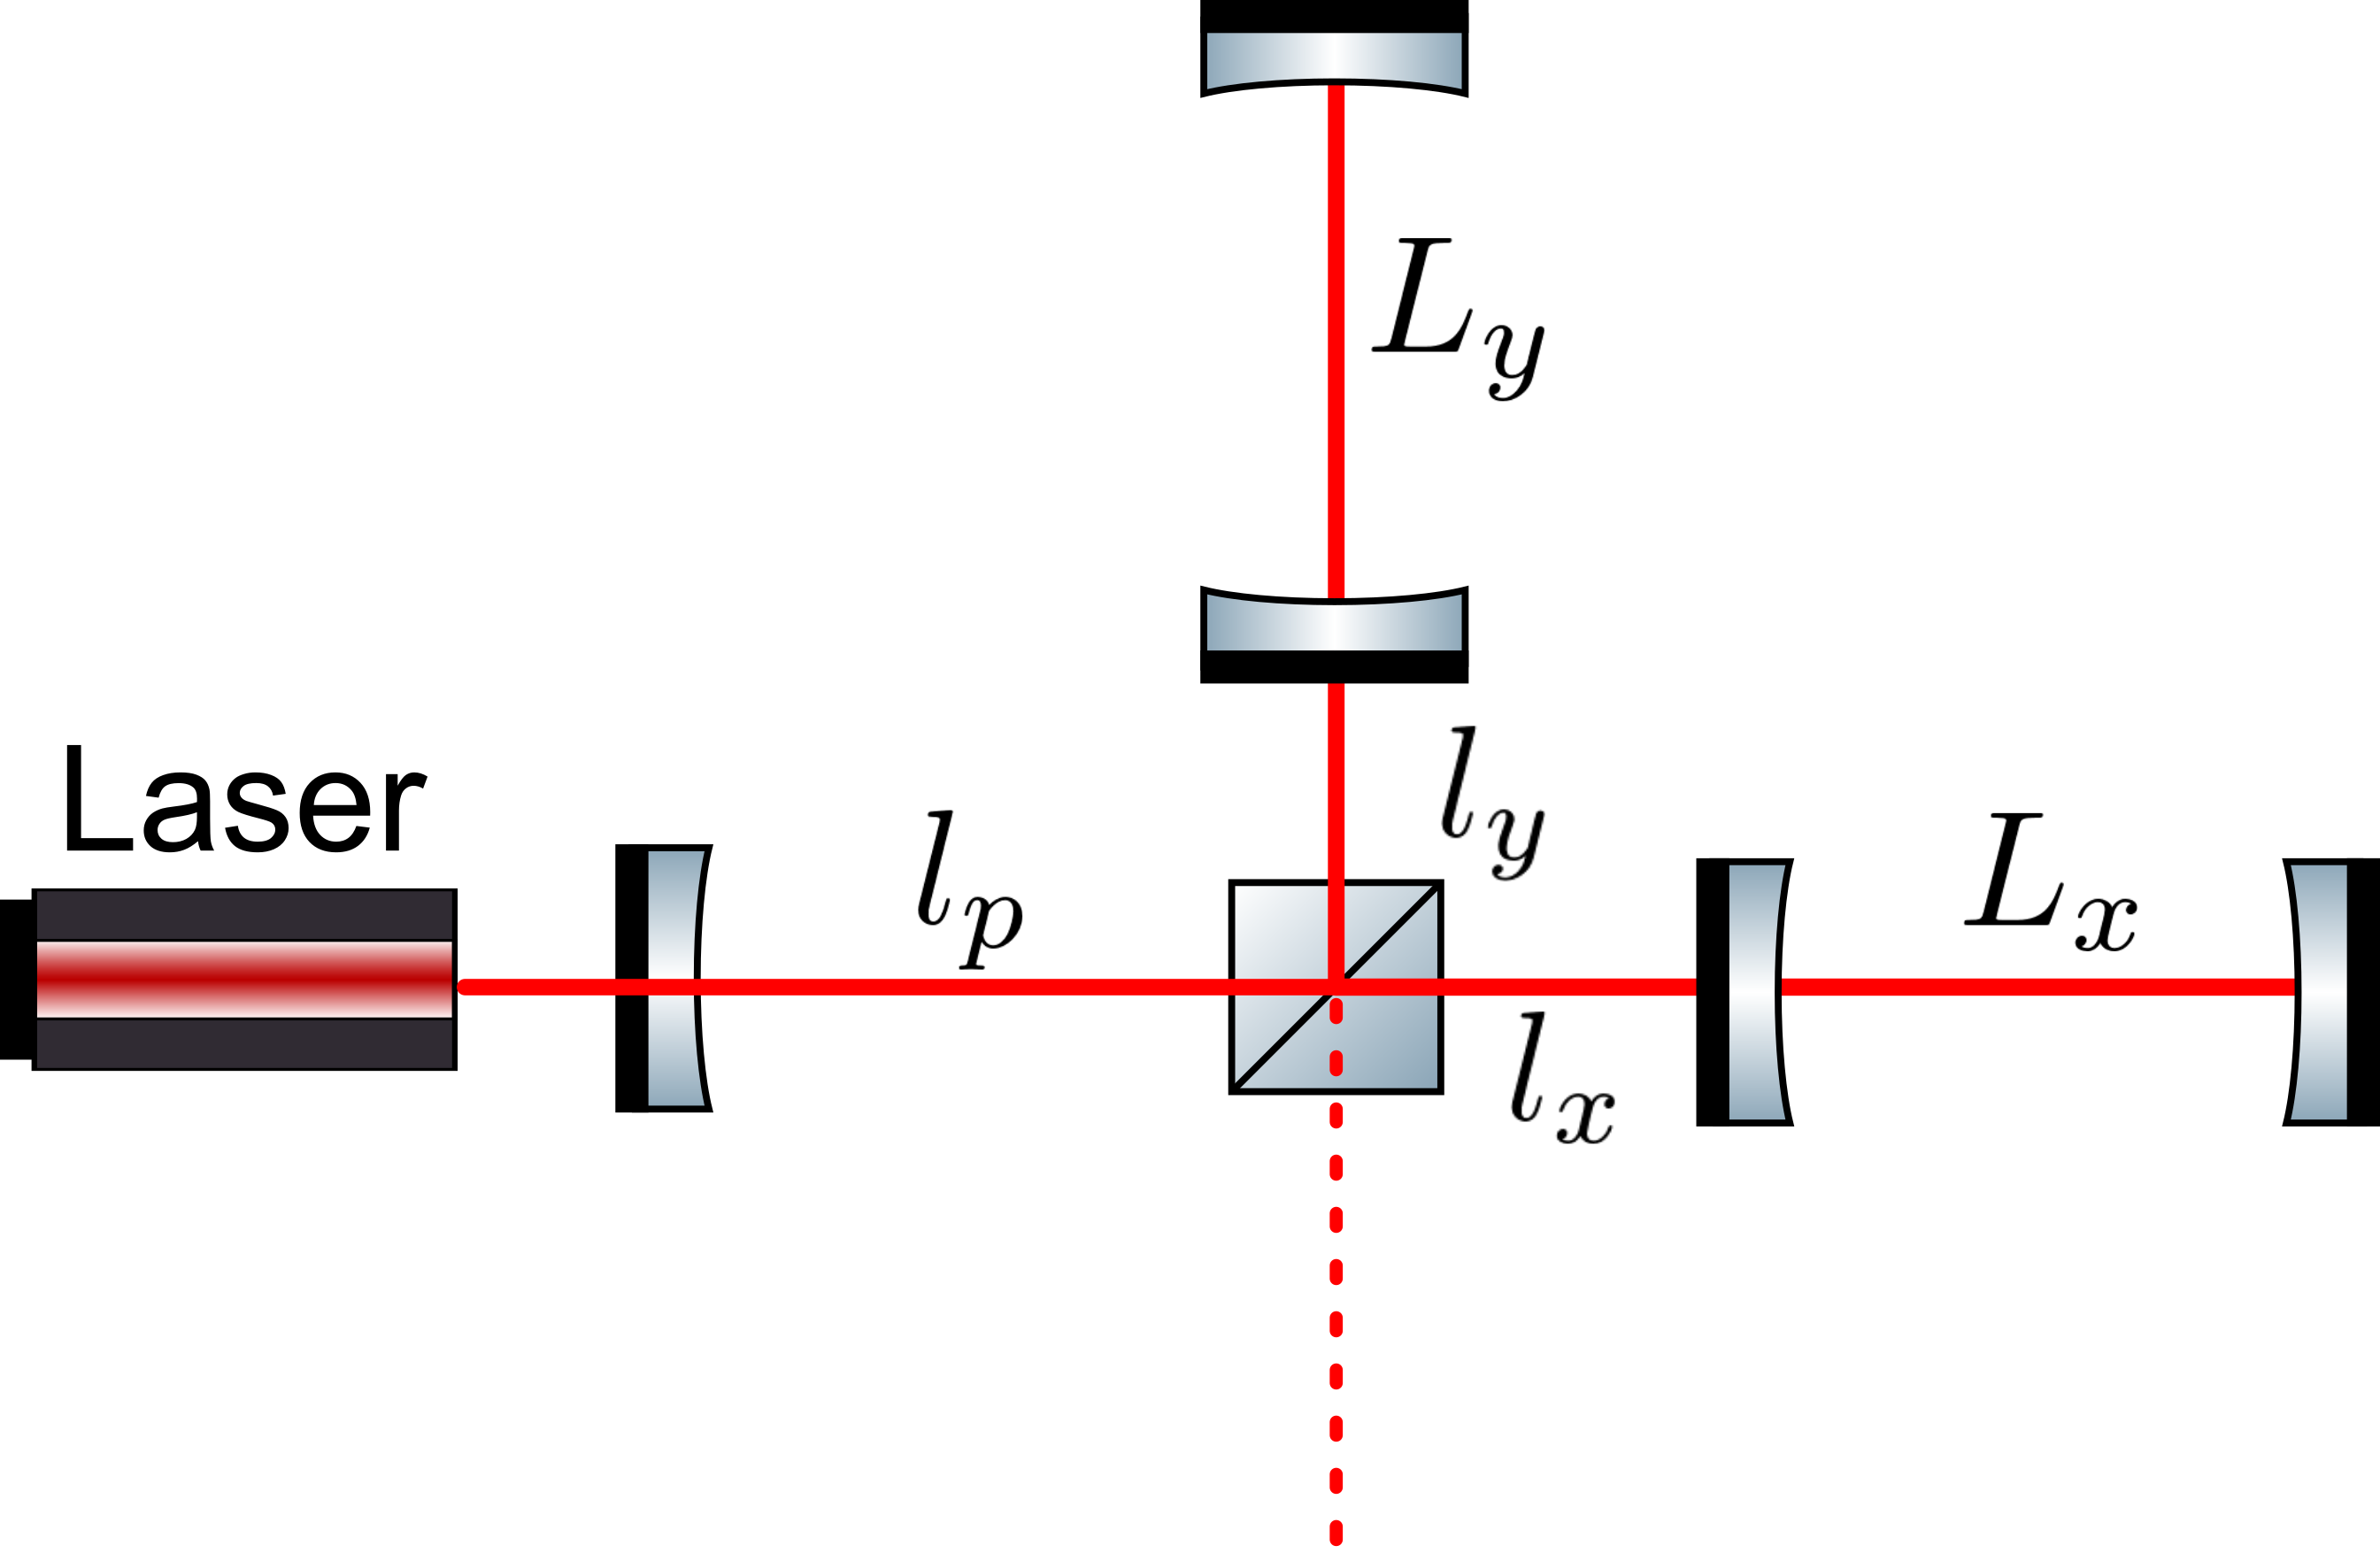
\includegraphics[width=\textwidth]{../Figures/PRFP_Mich.png}
				\caption{Power Recycled Fabry Perot}
				\label{fig:PRFPMich}
			\end{subfigure}
			\hfill
			\begin{subfigure}[b]{0.3\textwidth}
				\centering
				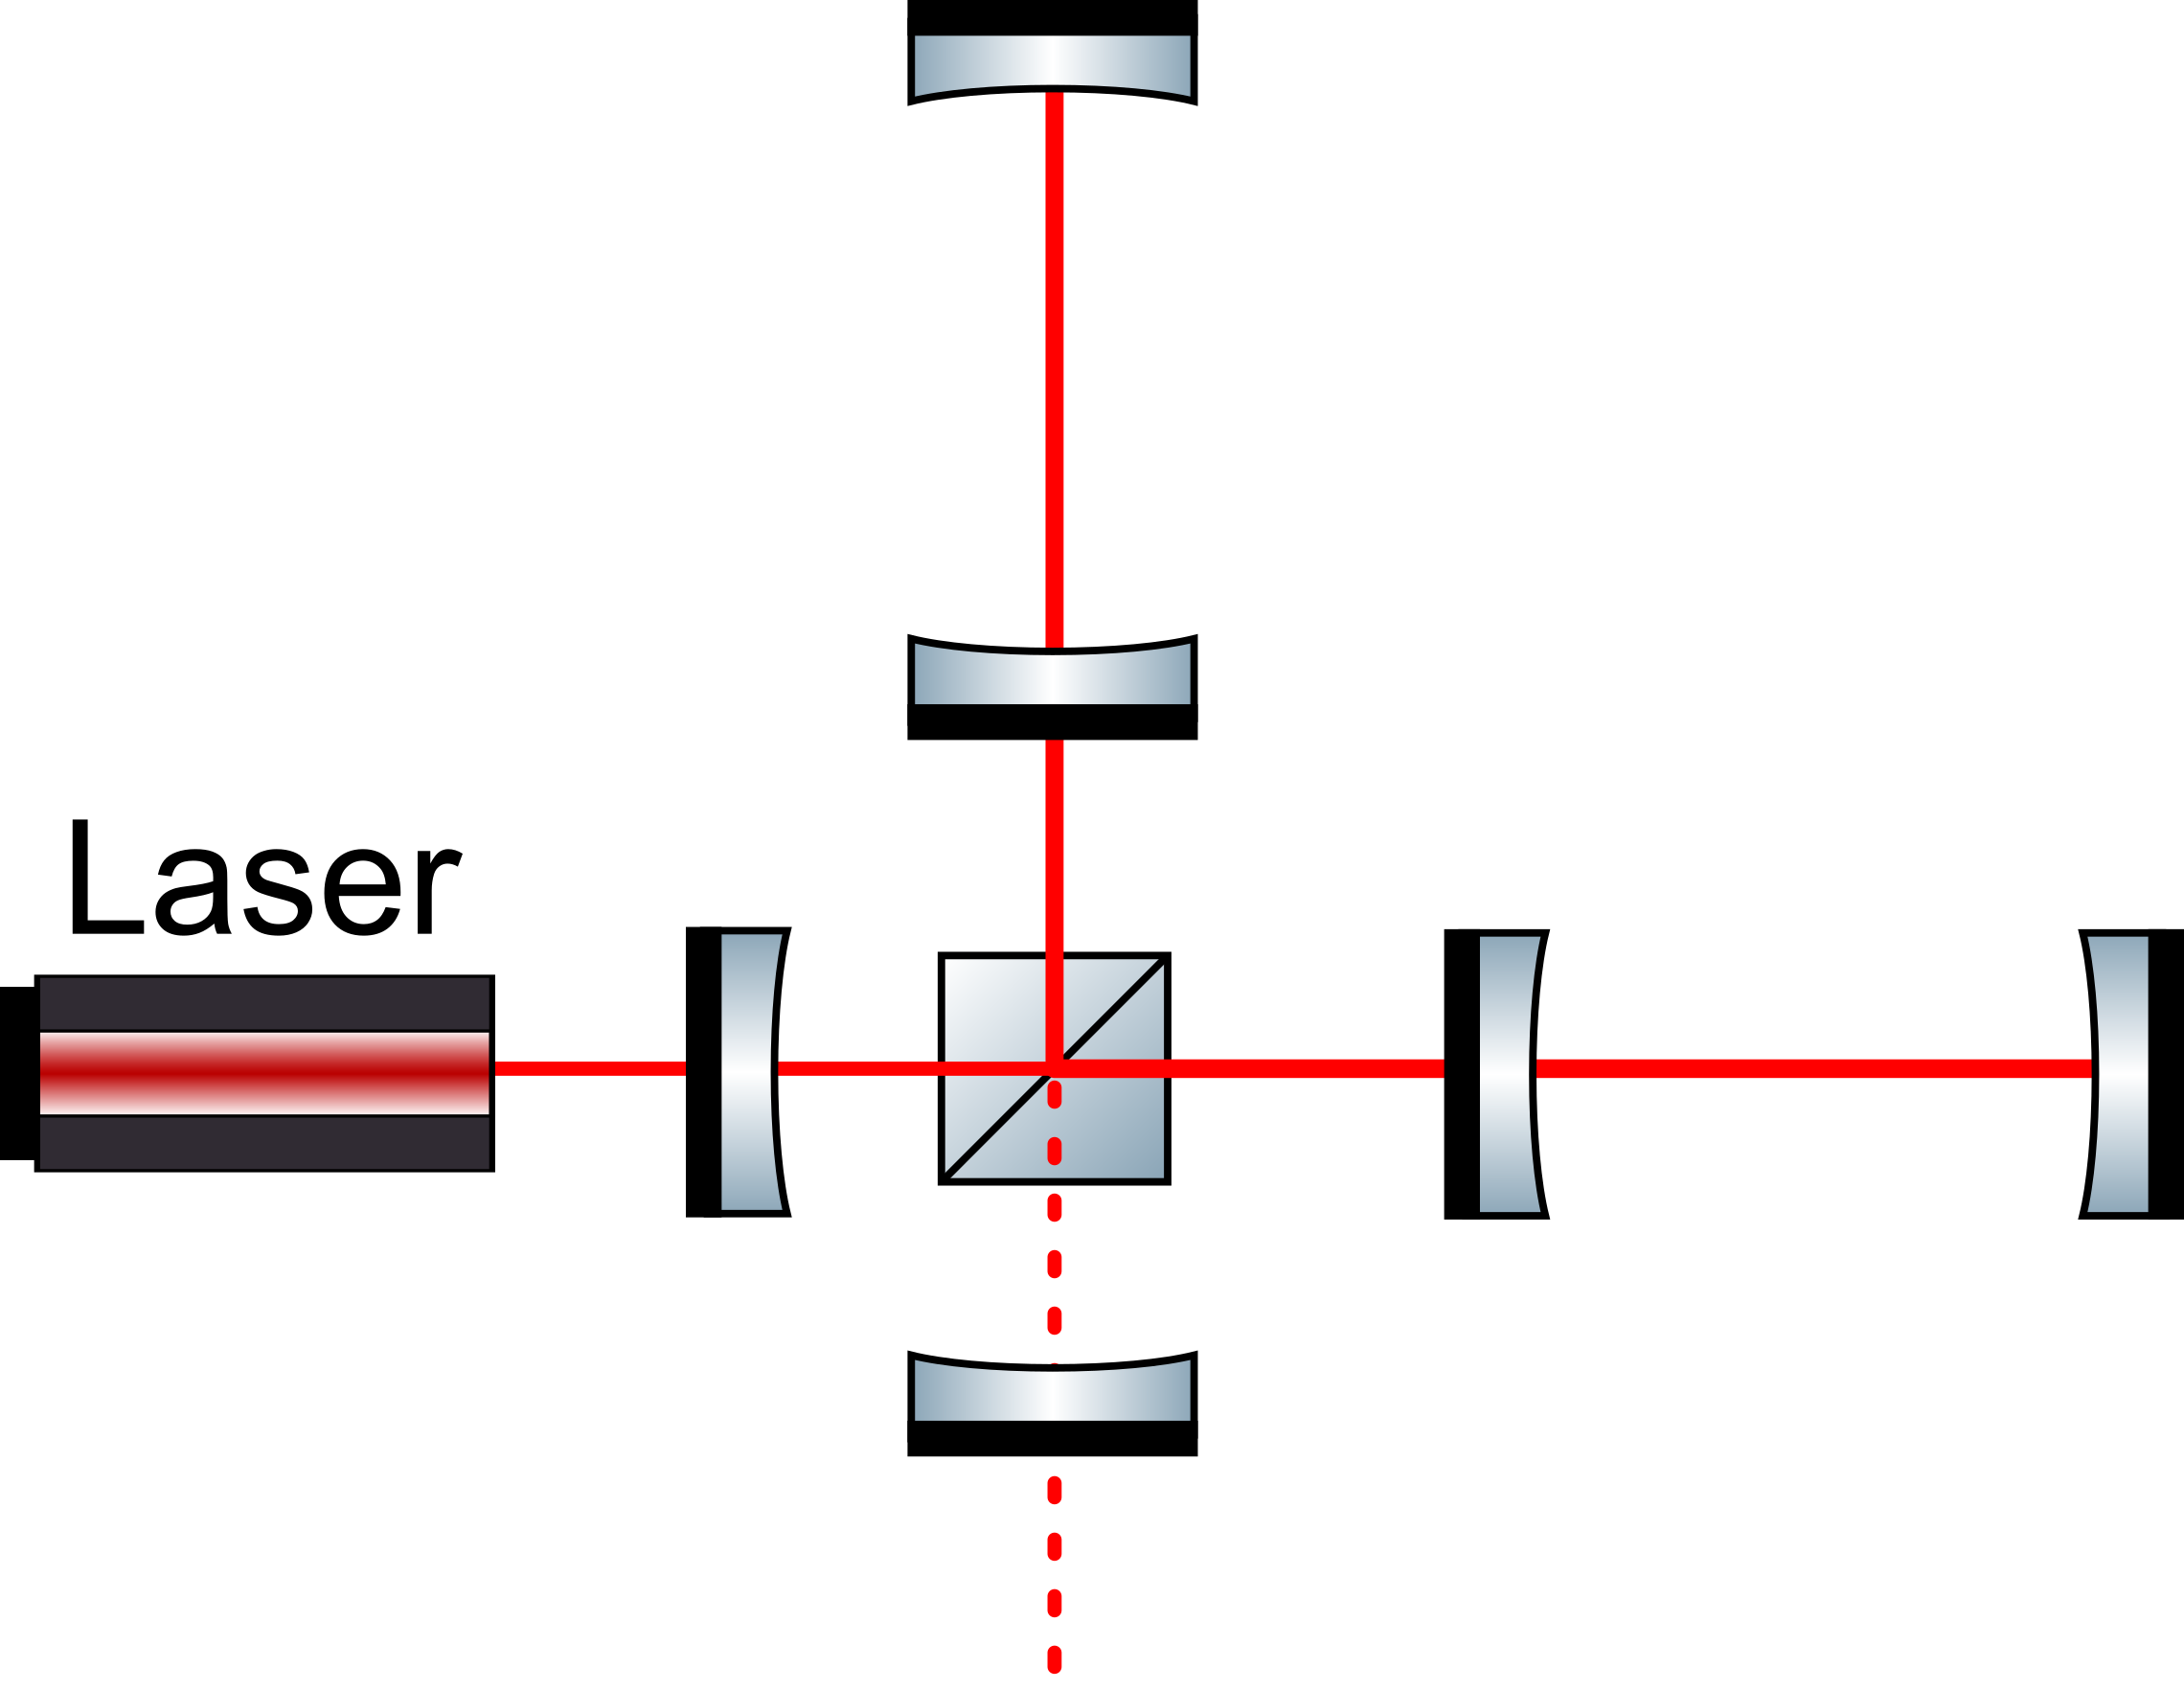
\includegraphics[width=\textwidth]{../Figures/DRFP_Mich.png}
				\caption{Dual Recycled Fabry-Perot}
				\label{fig:DRFPMich}
			\end{subfigure}
			\caption{Interferometer configurations}
			\label{fig:three graphs}
		\end{figure}

		If the interferometer is operating such that the intensity at the antisymmetric port is close to null, conservation of energy requires that the power from the arms will reflect back towards the input laser.  Fritschel et al [\cite{Fritschel_Readout} \cite{FritschelLightRecycling}] shows the effect of adding a partially reflecting mirror to increase the optical gain of the Michaelson for the sidebands and carrier fields.
		
		Section \ref{FPmich} showed that the Michelson interferometer with Fabry Perot arms can be represented by a single cavity response.  Therefore it is useful to model a power recycled interferometer by using a coupled cavity approach shown in Figure[PowerFPsimple] where the end mirror is replaced with the reflected field of the Michelson on a bright fringe.  Here the reflectivity and transitivity of the power recycling mirror (PRM) is denoted by $r_p$ and $t_p$, respectively.  
		
		In this configuration, the effective length of the cavity is
		the average path between the power recycling mirror and the high reflectivity surfaces of the input test masses,
		\begin{equation}
		l_{\text{PRC}} = l_\text{p} + \frac{l_x + l_y}{2}
		\end{equation}
		The circulating power in the cavity is given by equation \ref{c_FP} but uses the reflectivity of arm cavities,
		\begin{equation}
		E_{\text{PRC}} = \frac{t_p}{1- r_p r_{\text{FPM}}   e^{-2ik l_{\text{PRC}}}}E_{\text{in}}
		\end{equation}
		where $r_{\text{FPM}}\approx 1 - \frac{\mathbb{F}}{\pi} L_{\text{rt}} $ for high finesse cavities, which is a valid approximation for the advanced LIGO arm cavities since their values for finesse can be around 250 or higher depending on the losses.  This means the circulating power in the recycling cavity while on resonance can be expressed by
		\begin{equation}
		P_{\text{PRC}} = \frac{1-r_p^2}{\bigg[ 1 - r_p  (1 - \frac{\mathbb{F}}{\pi} L_{\text{rt}})   \bigg]^2}P_{\text{in}}
		\end{equation} 
		By taking the derivative with respect to the reflectivity of PRM and setting to zero, the optimal power recycling tuning is linearly proportional to the round trip loss,
		\begin{equation}
		r_{\text{opt}}  = 1 - \frac{\mathbb{F}}{\pi} L_{\text{rt}}
		\end{equation}
		so it important to keep the arm cavity losses as low as possible and this also limits the ability to increase the finesse.
		
		Adding a power recycling mirror will be equivalent to introducing higher power into the arm cavities but it will not shape the gravitational wave sideband frequency dependence in any other way.  This can be reasoned qualitatively by imagining the signal sidebands that get created in the arm cavities and propagate to the beam splitter where they will combine, however, the stretching and squeezing from the gravitational wave pattern will make the x-arm amplitude negative relative to the y-arm.  This makes the anti-symmetric port transmissive to the signal sidebands but the carrier field which mostly gets reflected to the symmetric port will see the power recycling amplification.  This means the beat note between the static carrier field and gravitational wave signal for a power recycled Fabry-Perot interferometer is
		\begin{equation}
		S_{\text{PRFP}} \propto E_0^2 \; \frac{8\pi L}{\lambda} \sqrt{g_{\text{PRC}}} \bigg[\frac{t_1}{1-r_1r_2}\bigg]^2 \bigg[\frac{1}{1 - i \frac{\omega_{\text{\tiny GW}}}{\omega_p}}\bigg] \sin{(k\delta l)} \sin{(\phi_{D})} h_{\text{\tiny GW}}
		\end{equation}
		where $g_{\text{PRC}} = P_{\text{PRC}}/P_{\text{in}}$ is the power recycling gain.
		
		\subsection{Dual-Recycled Fabry-Perot Interferometers}\label{DRMI}
		
		One of the biggest changes made between initial and advanced LIGO was the addition of a signal recycling mirror at the antisymmetric port (Figure [DRFPMI]). In the previous section, it was shown that the gravitational wave sensitivity was improved by adding a power recycling cavity to increase the effective input power into the Fabry-Perot cavities.  Adding another partially reflecting optic called the signal recycling mirror (SRM) at the antisymmetric port to create a resonant cavity will shape the interferometer's response to gravitational waves.  This allows for some flexibility in optimizing the instrument for specific sources such as binary neutron stars, but it also creates a more broadband response at higher frequencies while allowing the arm cavity finesse and/or power recycling to impart more power.
		
		\begin{figure}[ht]
			\centering
			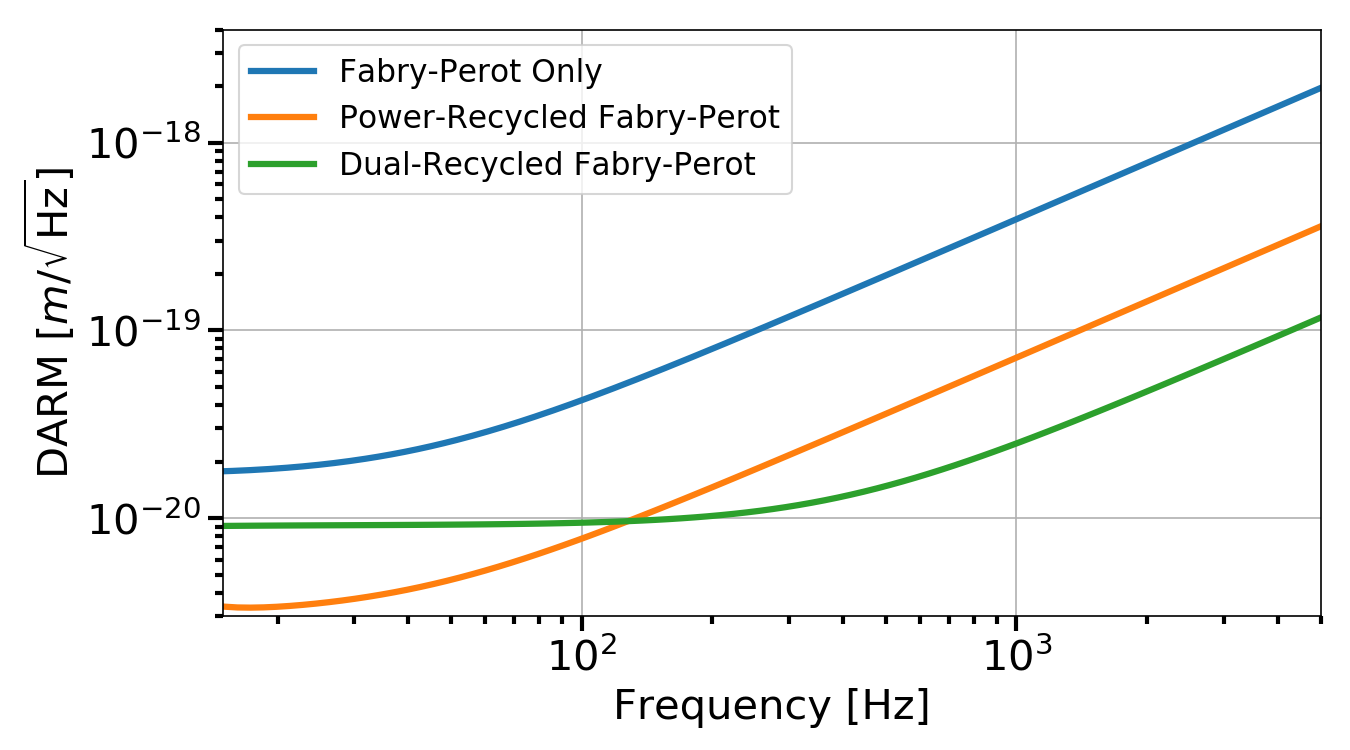
\includegraphics[width=1.0 \textwidth]{../Figures/SN_Lim_Sense.png}
			\caption{Shot noise limited sensitivity}
			\label{fig:SN_sense}
		\end{figure}
		
		\begin{figure}[ht]
			\centering
			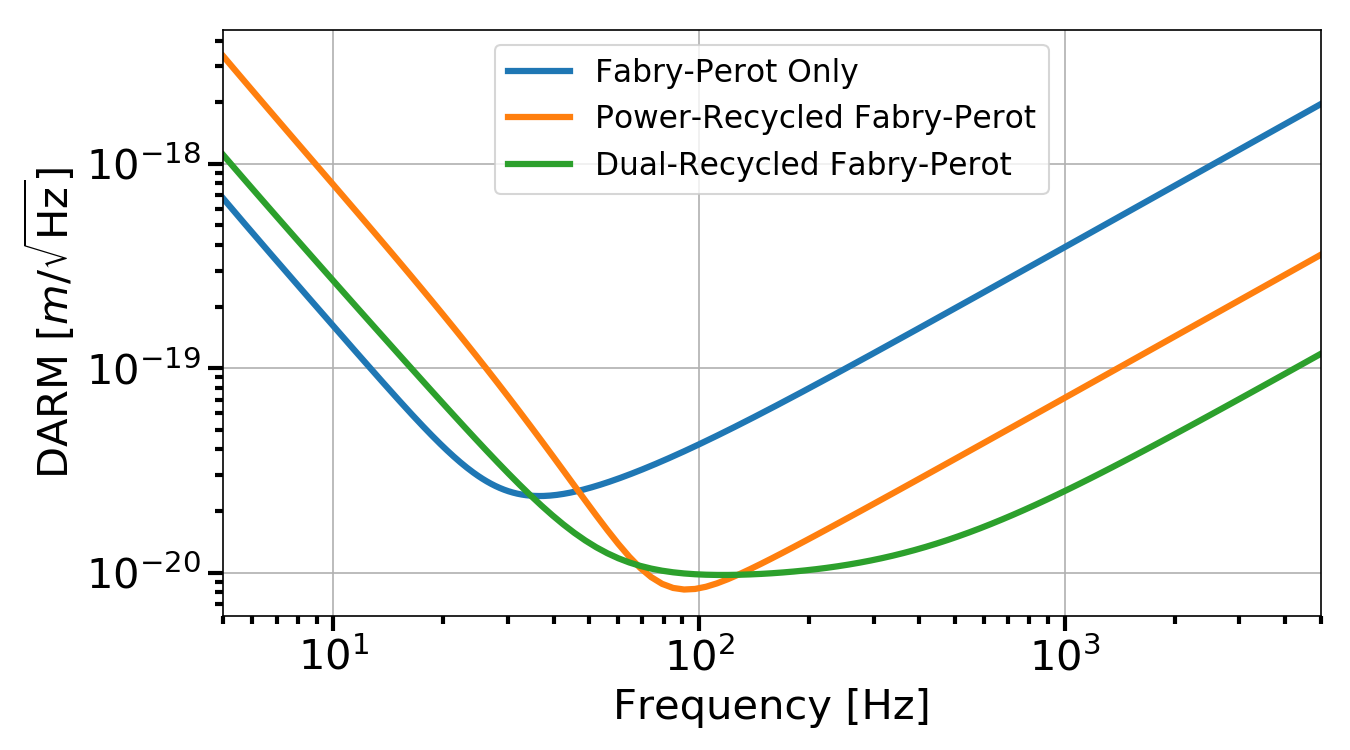
\includegraphics[width=1.0 \textwidth]{../Figures/QM_Limited_Sense.png}
			\caption{Quantum limited sensitivity by combining shot noise and radiation pressure}
			\label{fig:DRMICH_sense}
		\end{figure}
		
		A nice way to model the effect of signal recycling on the gravitational wave sidebands is to combine the SRM and  arm cavity input test mass to create a combined  mirror that is dependent on the round trip phase, $\phi_s$ of the signal recycling cavity.  The SRM will have a reflectivity and transmissivity equal to $r_s$ and $t_s$, respectively, so the combined mirror will have a reflectivity and transmissivity equal to
		\begin{equation}
		r_{1+s} = \frac{r_1 - r_s e^{-2i\phi_s}}{1- r_1 r_s e^{-2i\phi_s}}
		\end{equation}
		\begin{equation}
		t_{1+s} = \frac{t_1 t_s e^{i\phi_s}}{1- r_1 r_s e^{-2i\phi_s}}
		\end{equation}
		where $\phi_s = k \big( l_\text{s} + \frac{l_x + l_y}{2} \big)	$ is the average signal recycling length.
		Plugging this into equation \ref{Egw} in place of the input test mass reflectivity shows that the cavity pole is directly affected by the signal recycling properties, namely, the SRM reflectivity and the microscopic detuning of the length. The field propagating to the true antisymmetric port is in transmission of the signal recycling cavity which is accounted for with the last bracketed term. 
		\begin{equation}
		\begin{aligned}
		E_{\text{AS}}(\pm \omega_{\text{\tiny GW}}) & =  \bigg[ \frac{t_1^2}{1-r_1 r_2}\bigg]  \frac{E_0}{\sqrt{2}} \bigg[\frac{ 1}{1 \pm r_{1+s} r_2 e^{-2i  \omega_{\text{\tiny GW}}  \frac{L}{c}}} \bigg] \bigg[\frac{t_1 t_s e^{i\phi_s}}{1- r_1 r_s e^{-2i\phi_s}}\bigg] ik\Delta L\\
		& \propto \bigg[ \frac{ \text{Constant}}{1 \pm 2 i \frac{r_{1+s} r_2}{1- r_{1+s} r_2}  \omega_{\text{\tiny GW}}  \frac{L}{c}}  \bigg]\\
		& \propto \bigg[\frac{\text{Constant}}{1 \pm i \omega_{\text{\tiny GW}}/\omega_{\text{DR}}}\bigg]
		\end{aligned}
		\end{equation}
		Here, the frequency dependence of the differential cavity pole with dual recycling is denoted by
		\begin{equation}
		\begin{aligned}
			\omega_{\text{DR}} 	&=	\frac{1-r_{1+s}r_2}{r_{1+s}r_2}\frac{c}{2L}\\
								&=	\frac{1- r_1r_s e^{-2i\phi_s} }{ (r_1 - r_s e^{-2i\phi_s})r_2} - 1
		\end{aligned}
		\end{equation}
		
		Figure[ifoconfigs]
		The carrier field will also see a gain from the signal recycling cavity equal to
		\begin{equation}
		\sqrt{g_{\text{SRC}}} = \frac{t_s}{1+ r_s r_{\text{FPM}}   e^{-2i\phi_s}}
		\end{equation}
		It is clear from the equations above that the gravitational wave sideband and carrier fields will see the signal recycling cavity effects differently and the responses are highly sensitive to the length detuning of $\phi_s$.
		Putting all the pieces together to get the dual recycled Fabry-Perot interferometer response to gravitational waves,
		\begin{equation}
		S_{\text{DRFP}} \propto E_0^2 \; \frac{8\pi L}{\lambda} \sqrt{g_{\text{PRC}}}\;\sqrt{g_{\text{SRC}}}\; g_{\text{ARM}} \bigg[\frac{1}{1 - i \frac{\omega_{\text{\tiny GW}}}{\omega_{\text{DR}}}}\bigg] \sin{(k\delta l)} \sin{(\phi_{D})} h_{\text{\tiny GW}}
		\end{equation}

		

		The previous sections only considered the effect of Fabry-Perot cavities and recycling mirrors at the antisymmetric port due to a differential length change at the 4 kilometer arms but the Advanced LIGO interferometer has a few different degrees of a freedom which are actively controlled.  This means the signals sampling various ports will have contributions from one or more degrees of freedom.  A good reference for what is expected at the important ports such  as REFL, AS, and POP can be found in \cite{kiwamu_freq1} \cite{kiwamu_freq2} \cite{kiwamu_freq3}
		\subsection{Fundamental Noise Sources}\label{funnoise}
		The proceeding sections describe ways to increase the response of LIGO to gravitational waves; equally as important is the science of characterizing and reducing the noise contributions from everything else to optimize the sensitivity.
		
		\subsubsection{Quantum Noise}\label{Sec:QuantumNoise}
		Virtually all undergraduate quantum mechanics textbooks include a section on the harmonic oscillator [\cite{Shankar}].  An interesting result when solving the Schrödinger equation using creation ($\hat{a^{\dagger}}$) and annihilation $\hat{a}$ operators is the existence of a non-zero energy ground state which has variances in momentum and position related by the Heisenberg uncertainty principle.
		
		One fundamental noise source that is limiting LIGO's sensitivity comes from the fluctuations of quantum vacuum entering the anti-symmetric port and coupling to the input laser. A quantum mechanical description of an interferometer was constructed by Caves \cite{CavesQMNoise}\cite{Caves2photon} \cite{CavesOscillator}, where he used electric field operators to show that vacuum fluctuations are the cause of radiation pressure and shot noise in an interferometer.  Since then, there has been an explosion of research efforts associated with lowering the noise contributions from vacuum fluctuations by changing the interferometer configurations \cite{BuonannoChenQMNoise} \cite{ChenQND}.
		
		\textbf{Quantum states}:
		It is well known in physics \cite{Shankar} \cite{Griffiths} that a solution to the quantum harmonic oscillator in the energy eigenbasis employs the annihilation and creation  operators, $\hat{a}^{\dagger}$ and $\hat{a}$, to factorize the Hamiltonian
		\begin{equation}
		\hat{H} = \hbar w (\hat{N} + 1/2)
		\end{equation} 
		where $\hat{N} = \hat{a}^{\dagger}  \hat{a}$ is the number operator.  When using this formalism to create a coherent electromagnetic field, it is useful to define a unitary operator that displaces the vacuum state \cite{GerryKnight}:
		\begin{equation}
		\hat{D} \equiv \hat{D}(\alpha) \equiv \text{exp}(\alpha \hat{a}^{\dagger} - \alpha^{*} \hat{a} ) = e^{-\frac{\vert{\alpha}\vert^2}{2}} e^{\alpha \hat{a}^{\dagger} } e^{\alpha^{*} \hat{a} }
		\end{equation}
		
		
		$\hat{D}(\alpha) = \hat{D}^{-1}(\alpha) = \hat{D}(-\alpha)$
		\begin{equation}
		\begin{aligned}
		\hat{D}^\dagger&\, \hat{a} 		\,\hat{D}			= \hat{a} + \alpha \\ 
		\hat{D}^\dagger&\, \hat{a}^\dagger \,\hat{D} 		= \hat{a}^\dagger + \alpha^*
		\end{aligned}
		\end{equation}
		
		When applying the displacement operation on the vacuum state, the resultant vector has an amplitude $\alpha$ and follows the same uncertainty distribution as an unperturbed vacuum vector as shown in Figure[StickandBall],
		\begin{equation}
		\ket{\alpha} = \hat{D} \ket{0} =  e^{-\frac{\vert{\alpha}\vert^2}{2}} e^{\alpha \hat{a}^{\dagger} } \ket{0}
		\end{equation}
		
		\textbf{Radiation Pressure}
		
		One might naively think that power fluctuations in the laser cause radiation pressure effects on the test masses which will result in noise.  However, if the 50/50 beamsplitter is perfect, then the momentum transfer to each test mass will be a common length change and will not vary the intensity at the antisymmetric port (or the symmetric port for that matter).
		
		The concept of quantum radiation pressure arises from considering plane wave waves entering the interferometer from both the symmetric and anti-symmetric ports.  This method is similar to the input-output methods of section \ref{michelson}, however, the difference being that the beamsplitter will couple the electric fields from the input laser and quantum vacuum.
		
		To start, consider the electric fields combining at the beamsplitter from both ports to strike the mirrors, respectively,
		\begin{subequations}\label{exey}
		\begin{equation}
		E_x = \frac{1}{\sqrt{2}} \bigg[ iE_0 +   E_{AS,in} \bigg]
		\end{equation}
		\begin{equation}
		E_y = \frac{1}{\sqrt{2}} \bigg[  E_0 + i E_{AS,in} \bigg]
		\end{equation}
		\end{subequations}
		The intensities hitting each test mass will be
		\begin{subequations}
		\begin{equation}
		\vert E_x \vert^2 = \frac{1}{2} \bigg[ \vert E_0 \vert^2 + \vert E_{AS,in} \vert^2  + i(E_0 E^*_{AS,in} - E_0^*E_{AS,in} )\bigg]
		\end{equation}
		\begin{equation}
		\vert E_y \vert^2 = \frac{1}{2} \bigg[ \vert E_0 \vert^2 + \vert E_{AS,in} \vert^2  - i(E_0 E^*_{AS,in} - E_0^*E_{AS,in} )\bigg]`
		\end{equation}
		\end{subequations}
		
		The differential momentum transfer between the two masses will be equal to the differences in intensities:
		\begin{equation}\label{momentumtranfer}
		\begin{aligned}
		 \mathbf{P} 	&= \frac{2 \hbar \omega}{c} \bigg( \vert E_x \vert^2 - \vert E_y \vert^2 \bigg) \\
						&= \frac{2 \hbar \omega}{c} \bigg( E_0 E^*_{AS,in} - E_0^*E_{AS,in} \bigg)\\
		\Rightarrow	\mathbf{\hat{P}}&= \frac{2 \hbar \omega}{c} \bigg( \hat{a}_1^{\dagger} \hat{a}_2 - \hat{a}_2^{\dagger} \hat{a}_1 \bigg)
		\end{aligned}
		\end{equation}
		The last part of equation \ref{momentumtranfer} replaces the classical electric fields with creation and annihilation operators for the symmetric input mode ($\hat{a}_1^{\dagger}$, $\hat{a}_1$) and antisymmetric input mode ($\hat{a}_2^{\dagger}$, $\hat{a}_2$) modes. Recall that there is a well established convention denoting the wave function of the two dimensional modes of the quantum harmonic oscillator \cite{GerryKnight}, $\ket{\alpha,\beta}$, where $\alpha$ denotes the input symmetric mode and $\beta$ refers to the input antisymmetric mode.
		\begin{equation}
		\ket{\alpha,0} = \hat{D}_1(\alpha) \ket{0,0}
		\end{equation}
		The interesting results arising from this formulation is the expectation value
		\begin{equation}
		\langle \mathbf{\hat{P}} \rangle = \bra{\alpha,0} \mathbf{\hat{P}}\ket{\alpha,0} = 0
		\end{equation}
		And the variance 
		\begin{equation} 
		\begin{aligned}
		\Delta \mathbf{P}^2 &= \langle \mathbf{\hat{P}}^2 \rangle  - \langle \mathbf{\hat{P}} \rangle^2 \\
							&= \bigg(\frac{2 \hbar \omega}{c}\bigg)^2 \bra{\alpha,0}  \hat{a}_1^{\dagger}  \hat{a}_2  \hat{a}_1  \hat{a}_2^{\dagger} + \hat{a}_2^{\dagger}  \hat{a}_1  \hat{a}_2  \hat{a}_1^{\dagger}
							- \hat{a}_2^{\dagger}  \hat{a}_1  \hat{a}_1  \hat{a}_2^{\dagger} - \hat{a}_1^{\dagger}  \hat{a}_2  \hat{a}_2  \hat{a}_1^{\dagger} \ket{\alpha,0}\\
							&= \bigg(\frac{2 \hbar \omega}{c}\bigg)^2 \vert \alpha \vert^2
		\end{aligned}
		\end{equation}
		For some time interval, input laser power consisting of $\langle N \rangle =\vert\alpha \vert^2$ photons for a time interval $\Delta T$ is,
		\begin{equation}
		P_{in} = \frac{\hbar \omega}{\Delta T} \vert \alpha \vert^2
		\end{equation}
		To solve for the amplitude spectral density of the displacement, Newton's second law can be applied in the frequency domain
		\begin{equation}
		M (2\pi f)^2 \tilde{x}(f) = \tilde{F}(f) = \frac{\Delta \mathbf{P}}{\Delta T}
		\end{equation}
		The force spectrum is white because the impacting photons arrive randomly.
		
		Solving for the displacement,
		\begin{equation}
		\tilde{x}_{RP}(f) = \sqrt{\frac{\hbar \omega}{\Delta T} P_{in}} \frac{1}{2Mc (\pi f)^2}
		\end{equation}
	
		The noise spectral density for $M=40kg$, $P_{in}=125$W, and $\lambda=1064$nm
		\begin{equation}
		\tilde{h}_{RP}(f) = 2.04\times 10^{-20} \frac{1}{f^2} \; \bigg[ \frac{\text{Strain}}{\sqrt{\text{Hz}}}\bigg]
		\end{equation}
		\textbf{Shot Noise}
		Another way that quantum fluctuations can vary the antisymmetric port output is by adding phase noise.  Imagine holding the test masses rigidly such that the only effects on the output light is due to a phase change in the laser light in the arms. By using the same formulation for radiation pressure but propagating the fields back to the beam splitter, equations \ref{exey} will have extra phase,
		
		\begin{subequations}\label{exeyout}
		\begin{equation}
		E_{x,out} = \frac{1}{\sqrt{2}} \bigg[ iE_0 +   E_{AS,in} \bigg] e^{-i2kL_x}
		\end{equation}
		\begin{equation}
		E_{y,out} = \frac{1}{\sqrt{2}} \bigg[  E_0 + i E_{AS,in} \bigg] e^{-i2kL_y}
		\end{equation}
		\end{subequations}
		
		Antisymmetric port output electric field is
		\begin{equation}
		\begin{aligned}
		E_{AS,out} 	&= \frac{1}{\sqrt{2}} (E_{x,out} + iE_{y,out})\\
					&= i e^{-ikL_x-ikL_y} \big[\cos(\Delta \phi) E_0 - \sin(\Delta \phi) E_{AS,in}\big]
		\end{aligned}
		\end{equation}
		where $\Delta \phi = k(L_x-Ly)$
		Output intensity,
		\begin{equation}
		\begin{aligned}
		\mathbf{I}_{AS,out} 		&= \vert E_{AS,out}\vert^2 \\
									&= \bigg[ \cos^2(\Delta \phi)\vert E_0\vert^2 + \sin^2(\Delta\phi)\vert E_{AS,in}\vert^2 - \sin(\Delta\phi)\cos(\Delta\phi) \big[E_0 E^*_{AS,in} + E_0^* E_{AS,in}\big] \bigg]\\
		\Rightarrow	
		\hat{\mathbf{I}}_{AS,out} 	&= \bigg[ \cos^2(\Delta \phi)a_1^{\dagger}a_1 + \sin^2(\Delta\phi)a_2^{\dagger}a_2 - \sin(\Delta\phi)\cos(\Delta \phi) \big[a_1^{\dagger}a_2 + a_2^{\dagger}a_1 \big] \bigg]\\	
		\end{aligned}
		\end{equation}
		
		The expectation value for the intensity using an input coherent laser with $\alpha$ and quantum vacuum input at the antisymmetric port is
		
		\begin{equation}
		\begin{aligned}
		\langle \hat{\mathbf{I}} \rangle 	&= \bra{\alpha,0} \hat{\mathbf{I}}_{AS,out} \ket{\alpha,0}\\
							&= \cos^2(\Delta \phi) \vert \alpha \vert^2
		\end{aligned}
		\end{equation}
		
		which matches the classical description of a Michelson output.
		
		Following the same methods to calculate the radiation pressure, photon number variance is 
		\begin{equation} 
		\begin{aligned}
		\Delta \mathbf{I} 	&= \sqrt{\langle \mathbf{\hat{I}}^2 \rangle  - \langle \mathbf{\hat{I}} \rangle^2)} \\
							&= \vert \alpha \vert \big[ \cos^2(\Delta \phi)\ \big] 
		\end{aligned}
		\end{equation}
		\begin{equation}
		I = N \cos^2(\Delta \phi)
		\end{equation}
		\begin{equation}
		\frac{\partial I}{\partial \phi} = - 2 \vert \alpha \vert^2\cos(\Delta \phi) \sin(\Delta \phi)
		\end{equation}
		\begin{equation}
		\delta \phi = \sqrt{\frac{\hbar \omega}{ P_{in}}} \cot(\Delta \phi)
		\end{equation}
		Here $\delta \phi$ is the microscopic change in phase due to shot noise, whereas $\Delta\phi$ is the DC offset in the arm lengths to begin with. So in general, the shot noise contribution is dependent on the amount of light present at the anti-symmetric port and this will vary depending on what type of read out that is implemented.  To calculate the shot noise sensitivity, the phase shift in shot noise can be scaled by a factor of $\frac{\lambda}{2 \pi}\frac{1}{L}$ where $\lambda$ is the laser wavelength and $L$ is the DC length of the Michelson arms,
		\begin{equation}
		\tilde{h}_{SN}(f) = 8.2\times 10^{-22} \; \bigg[ \frac{\text{Strain}}{\sqrt{\text{Hz}}}\bigg]
		\end{equation}
		Unsurprisingly, the variance is proportional to the amount of photons present and the phase difference between the interferometer arms.
		Interestingly, there are a few subtleties associated with measuring the noise, it is assumed here that the interferometer readout is a simple photodetector located at the antisymmetric port.  However,it is possible to measure the light at two different phases (90 degrees apart) and subtract the results.   Also, in section \ref{michelson}, there is a freedom to choose the readout scheme of the interferometer (heterodyne or homodyne) which will also affect the overall quantum noise.
		
		\subsubsection{Seismic Noise}
		Reference:[Kissel Thesis]
		The main contributions to seismic noise are primarily caused by either natural occurrences  (tectonic plates, wind driven microcosms, oceanic storms etc) or man-made disturbances (heavy automotive traffic, industrial machinery, etc) which contribute to the background hum of motion.  Seismic noise will be the low frequency barrier for all terrestrial gravitational-wave detectors.  One of the biggest upgrades from eLIGO to aLIGO was the increase in complexity for seismic isolation and suspensions.  Using multiple stages of actively controlled platforms, the noise contribution can be attenuated for frequencies larger than ~1Hz;  in addition, the use of quadruple pendulums to hang the main arm cavity optics further reduces the motion above the pendulum's resonance frequency. This is a tremendous upgrade from the mostly passive isolation methods used in initial LIGO.
		
		Compare low and high noise microseisms
		\cite{BlairBook}
		The Advanced LIGO's solution to the low frequency wall is comprised of seismic isolation platforms and multi-level suspensions.
		
		\cite{driggers_global}
		
		\cite{fabrice_sei1}
		
		\cite{fabrice_sei2}
		
		\cite{fabrice_strat}
		
		\cite{sei_isol}
		
		\cite{Hang_LF}
		
		\cite{Fritschel_alignment}
		
		\subsubsection{Thermal Noise}
		Brownian motion \cite{brownian_einstein} is the random movement of particles suspended in a fluid.  The LIGO test masses, which make up the 4 kilometer long Fabry Perot cavities, are a large macroscopic object but their constituent atoms are excited by the ambient temperature and have associated random motion. Those atoms are interconnected and allow for the propagation of an infinite number of elastic wave modes that contain random relative phases and the linear superposition of the modes create distortions that result in thermal noise.	
		
		There are two important points that the Fluctuation-Dissipation theorem is based off:
		
		1) When in thermal equilibrium, a system's response to random fluctuations will be the same as when a small force applied.
		2) When a system dissipates energy, there exists a reverse process that allows energy to flow back into the system.
		
		A good way to start analyzing thermal noise is to consider a simple harmonic oscillator with mass $m$, that is in a thermal bath with a damping force, $F=-b\dot{x}(t)$.
		\begin{equation}
		\ddot{x}(t) + \gamma \dot{x}(t) + \omega_{0}^2 x(t) = F/m
 		\end{equation}
		Here, $\gamma = b/m$ and the force, $F$, can be described by white noise.  In this case, the force represents work being done on the system by the external world whereas the damping factor is the release of the system's energy to the outside world.  By taking the Fourier transform, the equation of motion becomes
		\begin{equation}\label{harmonic}
		\tilde{x}(f) = \frac{\tilde{F}(f)}{m} \; \frac{1}{\omega^2 +i \gamma \omega + \omega_{0}^2} 
		\end{equation}
		This implies that the spectral density for viscous damping is
		\begin{equation}\label{svis}
		S_{Vis} = \frac{S_F}{m^2} \; \frac{1}{(\omega^2 -\omega_{0}^2)^2 + (\gamma\omega)^2}
		\end{equation}
		Because the noise is due to a thermal bath, the integrated power over all frequencies must satisfy this equation
		\begin{equation}
		\frac{1}{2} \int_{-\infty}^{\infty} S_{Vis} (\omega) \frac{\text{d}\omega}{2\pi} = \frac{k_B T}{m\omega_{0}^2}
		\end{equation}
		where $k_B$ is the familiar Boltzmann's constant and $T$ is the ambient temperature.  Solving the integral and plugging the result for $S_F$ back into the equation \ref{svis} gives the power spectrum for viscous damping,
		\begin{equation}\label{vis}
		S_{Vis} = \frac{4k_B T \gamma}{m} \frac{1}{(\omega^2 - \omega_{0}^2)^2 + (\gamma\omega)^2}
		\end{equation}
		This equation shows that for three different frequency regimes, the response can vary wildly.
		\begin{subequations}
			\begin{equation}
			\omega<< \omega_{0} \rightarrow S_{vis} = \frac{4k_B T}{m Q \omega_{0}^3}
			\end{equation}
			\begin{equation}
			\omega \approx \omega_{0} \rightarrow S_{vis} = \frac{4k_B T}{m \omega_{0}^3} Q
			\end{equation}
			\begin{equation}
			\omega >> \omega_{0} \rightarrow S_{vis} = \frac{4k_B T}{m Q} \frac{\omega_0}{\omega^4} 
			\end{equation}
		\end{subequations}
		where $Q=\omega_{0}/\gamma$ is commonly known as the quality factor of a resonator.  Qualitatively, this is directly proportional to the resonance height and its thinness.  Figure [visthermalnoise] shows the resultant frequency dependent power spectrum for a few different quality factors, for higher $Q$ systems the amount of noise contribution from thermal noise is reduced at frequencies above the resonance.  Another commonly used definition of the quality factor is the amount of energy loss per cycle, if the $Q$ of a system is high, then the amount of energy loss per oscillation is very small and will take a longer time returning to equilibrium.  A good description of the quality factor and its application to gravitational wave detectors can be found in section 7.5 of \cite{Saulson}.
		
		As system's mode number increases, the previous analysis becomes very difficult to solve analytically. However, the connection between a damped harmonic oscillator's energy loss and power spectrum can be described generically using the Fluctuation Dissipation Theorem,
		\begin{equation}\label{FD}
		S_x(f) = \frac{k_B T}{\pi^2 f^2} \vert \operatorname{\mathbb{R}e} (Y(f)) \vert
		\end{equation}
		where $Y(f)$ is the complex mechanical admittance (inverse of the impedance) of a system. The physical interpretation of equation \ref{FD} can be viewed as a tunnel of energy between a system of interest and the outside world.  If there is an ability to couple energy from one system to another via some process, then the reverse must be true as well. This subtle but powerful statement can be applied generally.  For example, a resistor which is able to dissipate thermal energy when current is flowing through it will convert random external temperature fluctuations into stray currents that results in $Johnson$ $Noise$.
		
		The mechanical admittance of a system is defined as $Y(f) = \dot{x}(f)/F(f)$, which can be written down directly for a damped harmonic oscillator using equation \ref{harmonic},
		\begin{equation}
			\begin{aligned}
			\frac{\dot{x}(f)}{F} &= \frac{i \omega}{m} \frac{1}{\omega_{0}^2 - \omega^2 +i\gamma \omega}\\
								 &= \frac{i\omega}{m} \frac{(\omega_{0}^2 - \omega^2 - i \gamma \omega)}{(\omega_0^2 - \omega^2)^2 + (\gamma \omega)^2}
			\end{aligned}
		\end{equation}
		and by plugging this into the fluctuation dissipation theorem, the power spectral density matches equation \ref{vis} for the viscous damping.  To extend the usage further, consider the thermal noise from a solid which has some thermoelastic dissipation from an internal mode given by $F_{diss} = -k(1+\phi_L) x(t) $ where the phase term comes from the lag between applied force and the system's response to said force.  By solving Newton's second law with this new damping term, the displacement spectrum becomes 
		\begin{equation}
		\tilde{x}(f) =  \frac{\tilde{F}}{m} \; \frac{1}{(1 + i\phi_L ) \omega_{0}^2 - \omega^2 }
		\end{equation}
		Unlike the previous example of viscous damping, the integral for thermoelastic dissipation only holds for some frequency regime but implementing the fluctuation dissipation theorem leads directly to the noise power spectrum,
		\begin{equation}
			S_{TD}(f) =  \frac{4k_B T \omega_{0}^2 \phi_L}{m \omega} \frac{1}{(\omega^2 - \omega_{0}^2)^2 + (\omega_{0}\phi_L)^2}
		\end{equation}
		The frequency response will also be different compared to viscoelastic dissipation,
		\begin{subequations}
			\begin{equation}
			\omega<< \omega_{0} \rightarrow S_{vis} = \frac{4k_B T}{m Q \omega \omega_{0}^2}
			\end{equation}
			\begin{equation}
			\omega \approx \omega_{0} \rightarrow S_{vis} = \frac{4k_B T}{m \omega_{0}^3} Q
			\end{equation}
			\begin{equation}
			\omega >> \omega_{0} \rightarrow S_{vis} = \frac{4k_B T}{m Q} \frac{\omega_0^2}{\omega^5} 
			\end{equation}
		\end{subequations}
		The structural damping formalism can also be applied to the suspension fibers which hold the 40 kilogram test masses[\cite{SaulsonThermalSus}, \cite{Saulson}] which yield a noise spectral density that contains resonances at a variety of frequencies.  The lower two modes consist of the pendulum and rocking modes, while starting at 500 hertz the violin modes will be seen.  In fact, the violin modes and their harmonics could get rung up from earthquakes and saturate the output mode cleaner's DC photodiodes so the must be actively damped in order to proceed towards nominal low noise.
		
		The largest contribution to the thermal noise for current interferometers do not stem from viscous damping, thermoelastic damping of the substrate, or internal friction of the suspension fibers, but rather from the thermal noise contributed by the dielectric coatings [\cite{HarryThermalCoat}] which cause phase noise at the high reflectivity surface of the mirrors.
		
		
		Thermal Noise [\cite{SaulsonThermalNoise}]
		
		Suspension Thermal Noise \cite{SaulsonThermalSus}
		
		Substrate Thermal Noise [\cite{Saulson}]
		
		Coating Thermal Noise [\cite{HarryThermalCoat}]
		
		Thermal-Optical Noise[\cite{EvansBallmerThermalOptic}]
		
		Residual Viscous damping[\cite{Saulson}]
		
		\subsubsection{Newtonian Noise}
		Although there are some noise sources that can be reduced using increasingly complicated techniques such as various levels of seismic isolation or quantum non-demolition devices as shown above. [\cite{SaulsonNewtonian} and \cite{ThorneNewtonian}].  Newtonian noise caused by fluctuating gravitational fields from the wave motion of the ground is one that cannot easily be reduced but possibly be measured and fed-forward or subtracted off-line.[\cite{DriggersNewtonian}]

	\section{Mode Matching with Squeezed States of Light}
	In Section \ref{Sec:QuantumNoise}, the quantum limited sensitivity for a Michelson interferometer was shown to be comprised of shot noise and radiation pressure. Although quantum fluctuations are a fundamental noise source, their effects can be modified by manipulating the quantum vacuum with correlated photons and injecting these states of light into the antisymmetric port of the interferometer.  Within the LIGO community, this procedure of modifying quantum vacuum is called squeezing.  The production of squeezed states with nonlinear devices is a well understood subject and was successfully tested in the sixth LIGO science run \cite{LSCBeyondQM}\cite{LSCEnhancedSenseSqz}.  An extension of the formalism described in Section \ref{Sec:QuantumNoise} was developed by Caves-Schumaker \cite{Caves2photon} which describes two-photon quantum optics and squeezing, but it is outside of the scope in terms of mode matching. 
	
	However, it useful to understand the quantum noise in a formalism which scales the interferometer sensitivity in terms of the $\textit{Standard Quantum Limit}$ (SQL).   The radiation pressure and shot noise add in quadrature to form the quantum noise and both are proportional to the square root of the input power but in different regimes.  The SQL refers to the input power minimizes the total quantum noise and is the minimum achievable noise without squeezing.  The radiation-pressure back-action coupling constant, $\kappa$, is given by \cite{KimbleConversion}
	\begin{equation}
	\kappa = \frac{4 P_0 \omega_{0}}{m c^2 f^2}
	\end{equation}
	where $P_0$ is the input power on the beamsplitter, $\omega_{0}$ is the laser angular frequency, $m$ is the optic mass, and $f$ is the Fourier domain frequency.  The SQL for a simple Michelson is given by \cite{KimbleConversion},
	\begin{equation}
	S_{SQL} = \frac{4 \hbar}{m L^2 f^2}
	\end{equation}
	With these two equations above, the total single-sided power spectral density for a simple Michelson is
	\begin{equation}
	S_{SM} = \frac{S_{SQL}}{2} \bigg( \frac{1}{\kappa}  + \kappa\bigg)
	\end{equation}
	Here the first term is represents the shot noise while the second term is the radiation pressure contribution. 
	\begin{figure}[ht]
		\centering
		\begin{subfigure}[b]{0.45\textwidth}
			\centering
			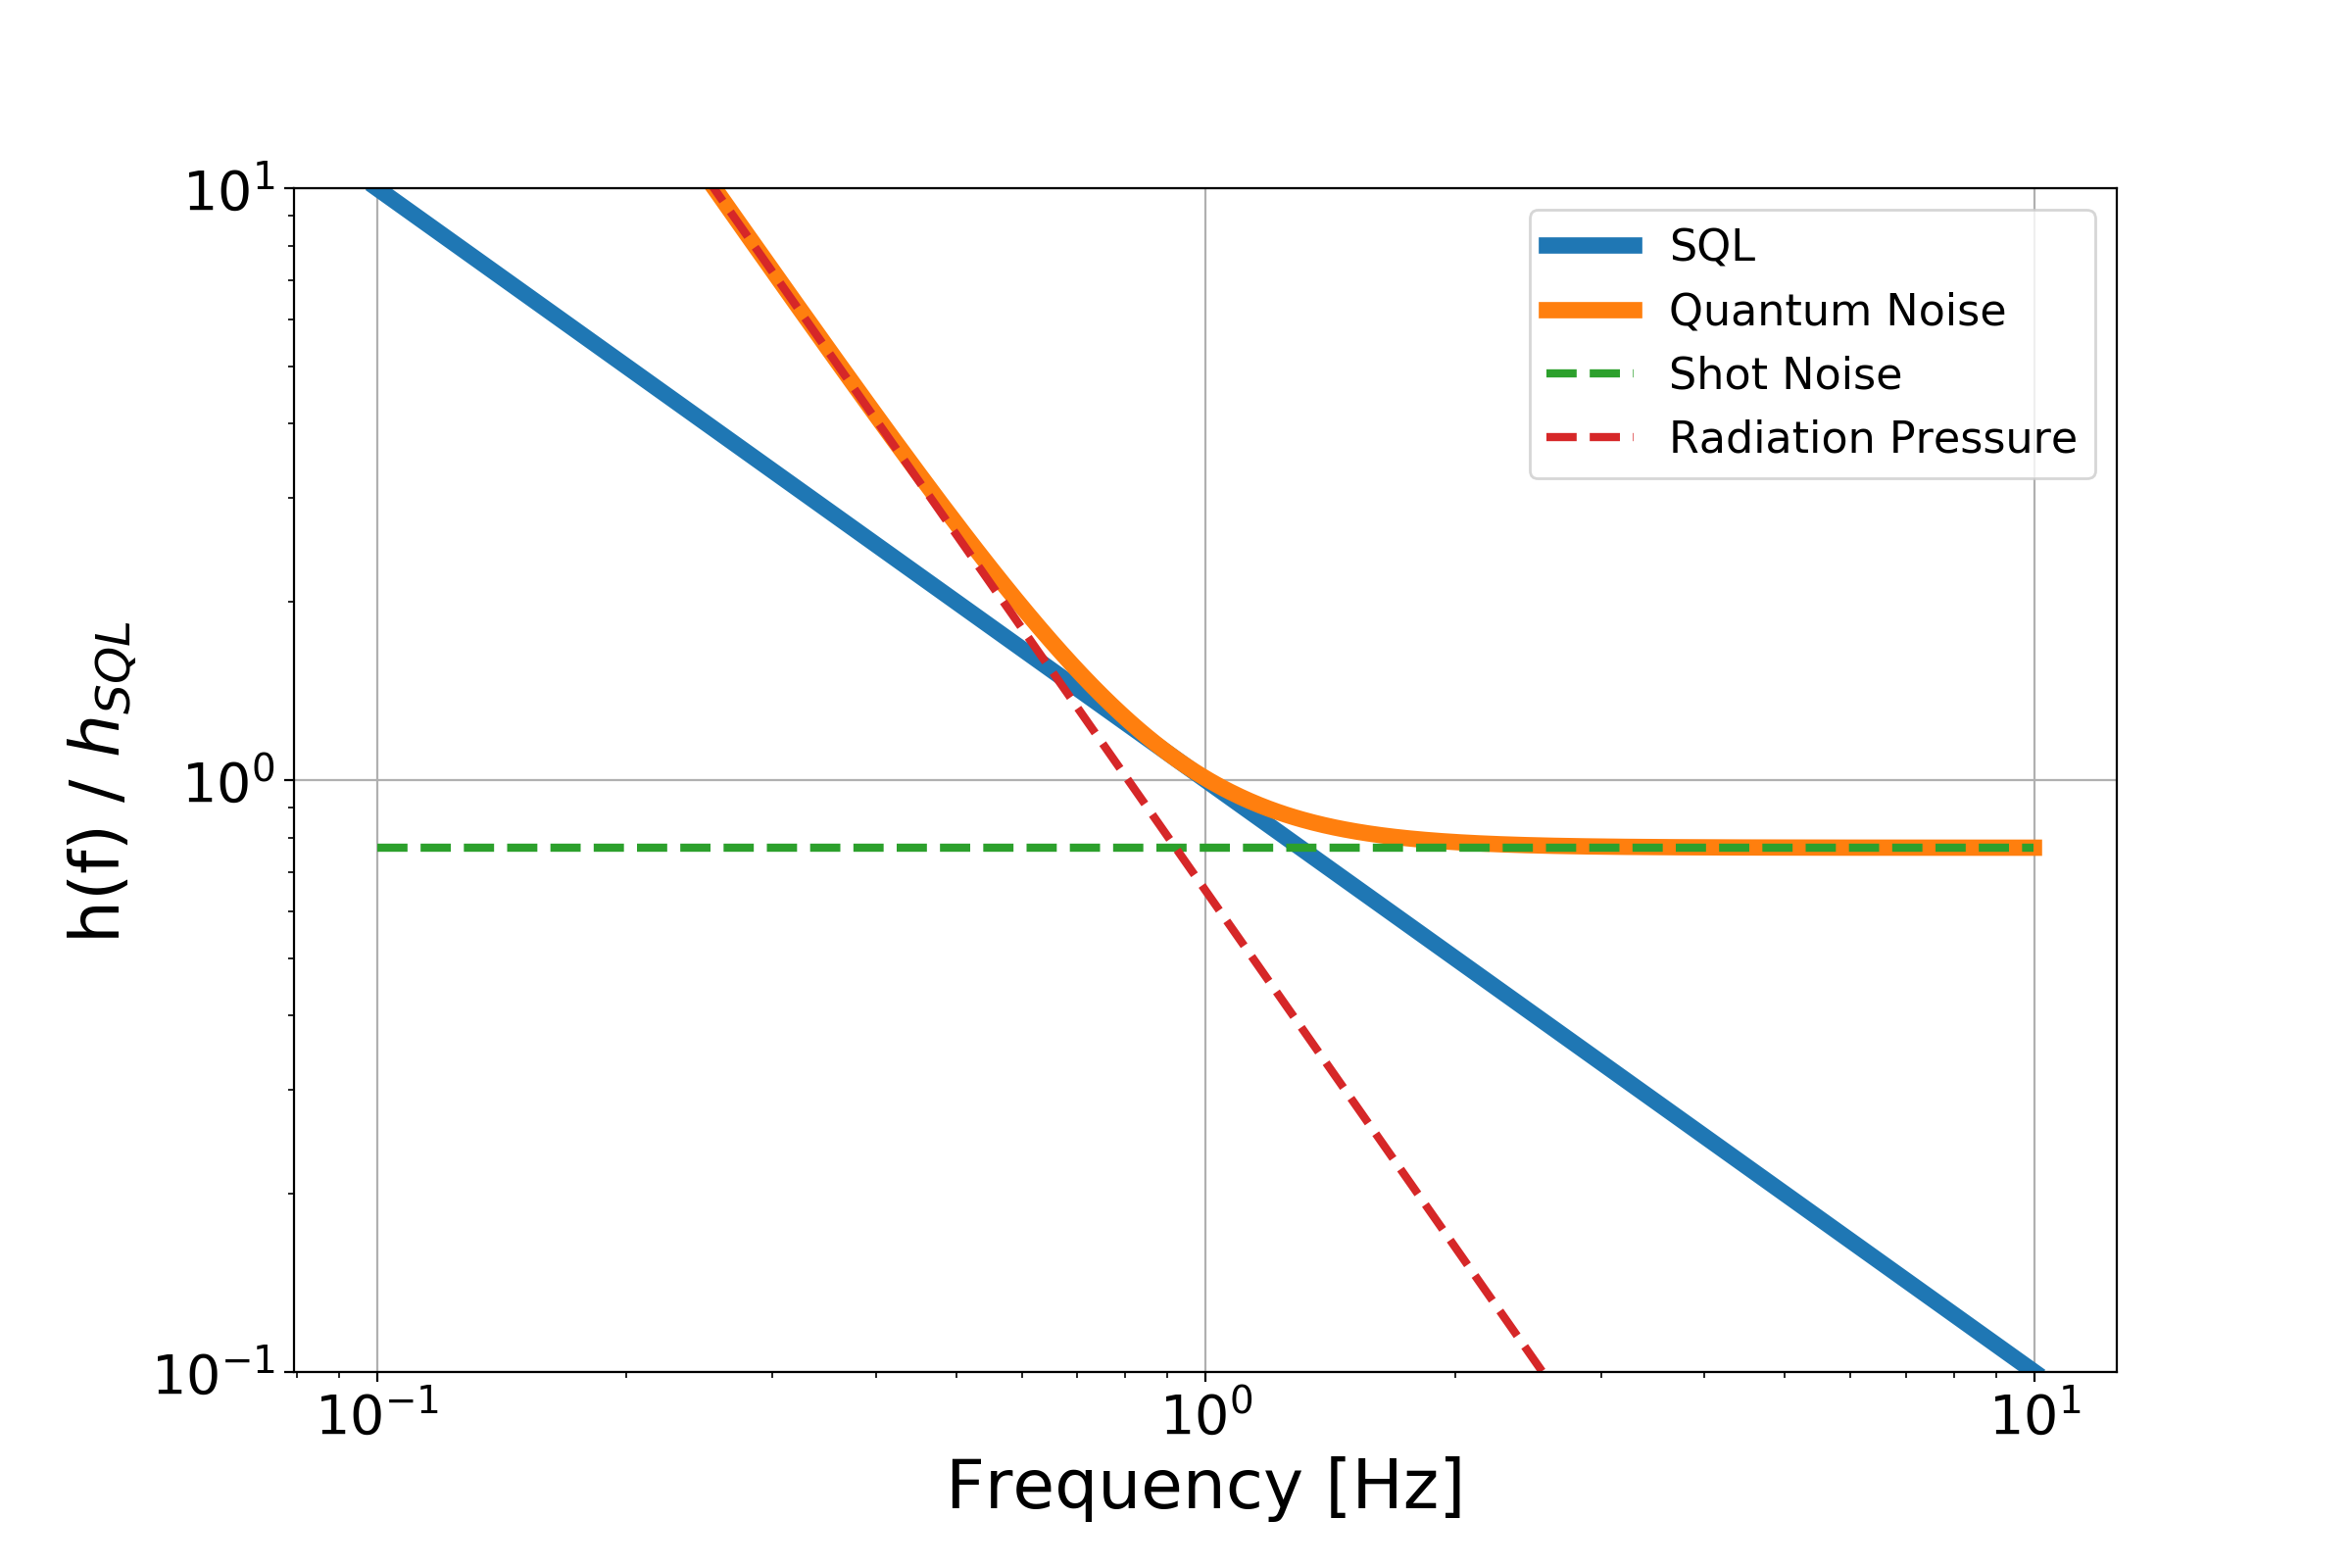
\includegraphics[width=\textwidth]{../Figures/Kimble_SM_QM.png}
			\caption{Simple Michelson quantum noise}
			\label{fig:kimble_SM}
		\end{subfigure}
		\hfill
		\begin{subfigure}[b]{0.45\textwidth}
			\centering
			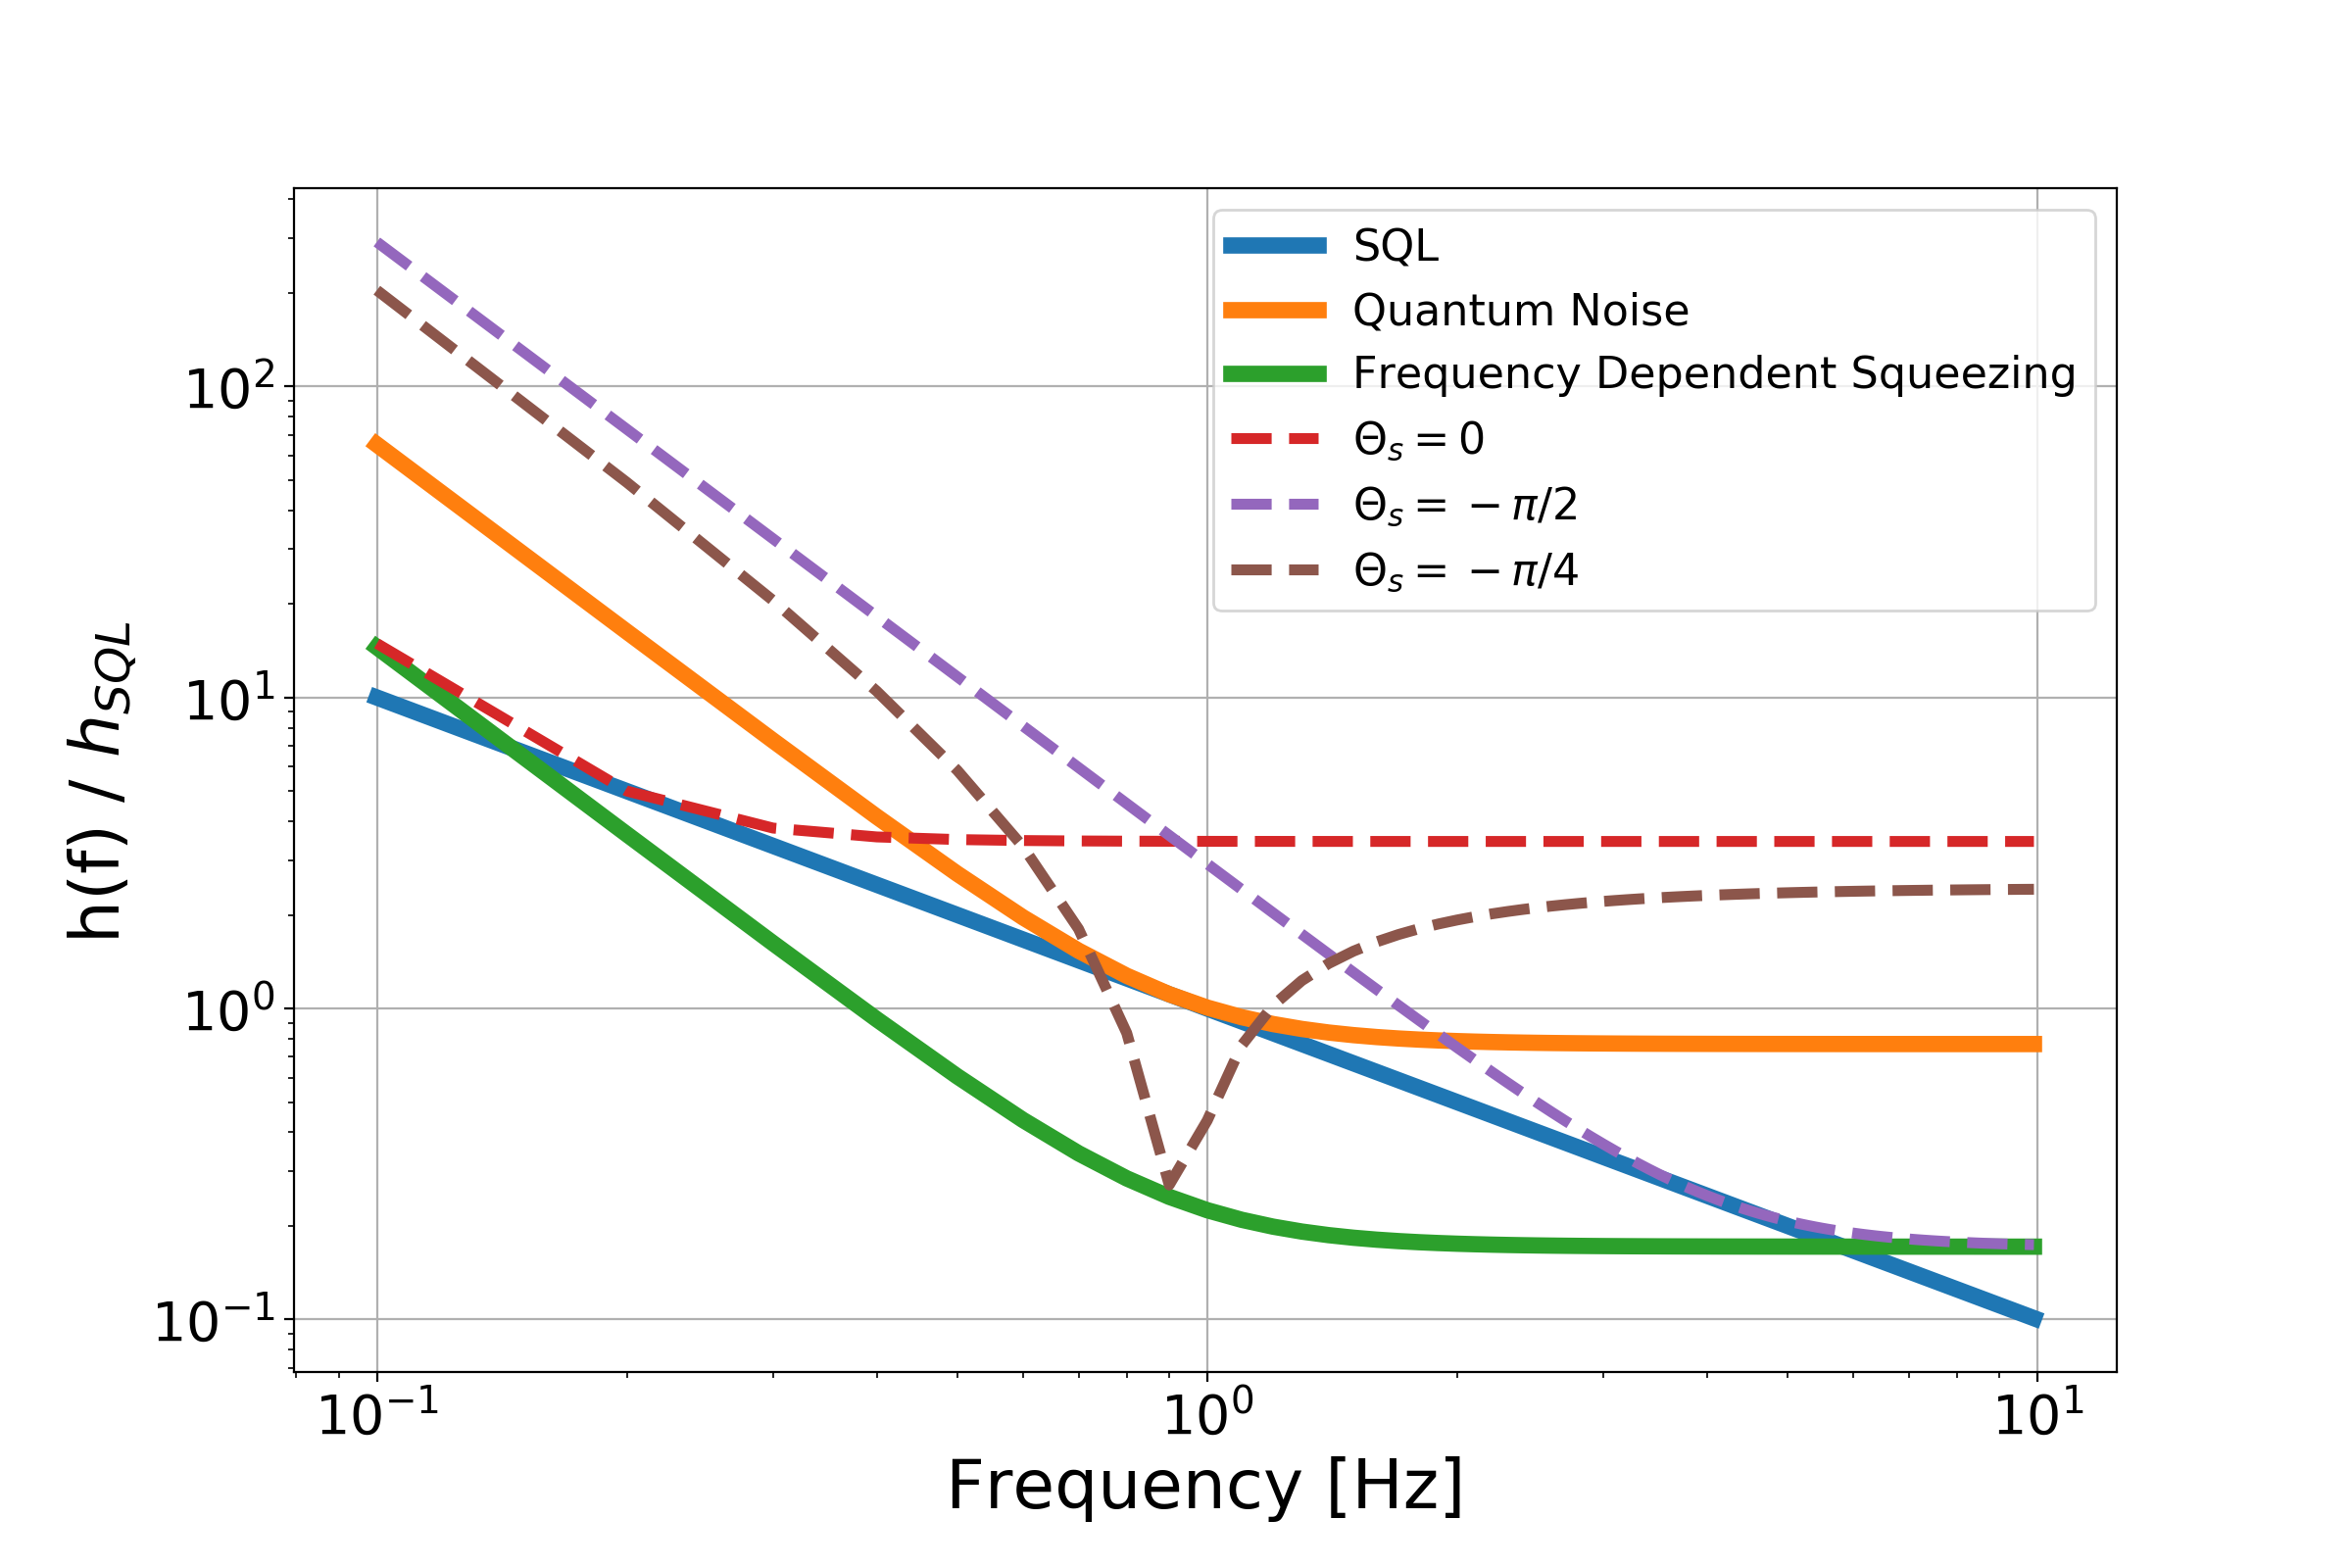
\includegraphics[width=\textwidth]{../Figures/Kimble_SM_QM_sqz.png}
			\caption{Simple Michelson quantum noise with squeezing}
			\label{fig:kimble_SM_sqz}
		\end{subfigure}
		\caption{The amplitude spectral density of gravitational wave strain normalized by the standard quantum limit.}
		\label{fig:PSD_SM}
	\end{figure}
	
	Modifying the field entering the antisymmetric port by replacing the quantum vacuum with a squeezed state has interesting effects on the strain sensitivity and reduces the noise floor below the standard quantum limit. The power spectral density for a simple Michelson with injected squeezing is described by \cite{KimbleConversion}
	\begin{equation}
	\begin{aligned}
	S_{SM Sqz} 	&=  \frac{S_{SQL}}{2} \bigg( \frac{1}{\kappa}  + \kappa\bigg) [\cosh{2R} - \cos(2(\phi_s+\theta_s)) \sinh{2R}]\\
	&= \frac{S_{SQL}}{2} \bigg( \frac{1}{\kappa}  + \kappa\bigg) e^{-2R} \qquad \text{for } \theta_s = -\phi_s
	\end{aligned}
	\end{equation}
	where $R$ is the squeeze factor, $\theta_s$ is the squeeze angle, and $\phi_s = \cot^{-1}(\kappa)$.  The squeeze angle can change the regime of strain which is affected, for example, when injecting for optimal shot noise reduction one would choose $\theta_s=\pi/2$.  However, when trying to reduce the radiation pressure noise, then choosing $\theta_s=0$ is optimal.   For the second line in the equation above, to achieve broadband squeezing, the squeeze angle must be rotated as a function of frequency.  Fortunately, this can be achieved by reflecting the squeezer beam off a filter cavity before injecting into the interferometer \cite{Oelker_FD_sqz} \cite{EvansRealistic}.
	
	\begin{figure}[ht]
		\centering
		\begin{subfigure}[b]{0.5\textwidth}
			\centering
			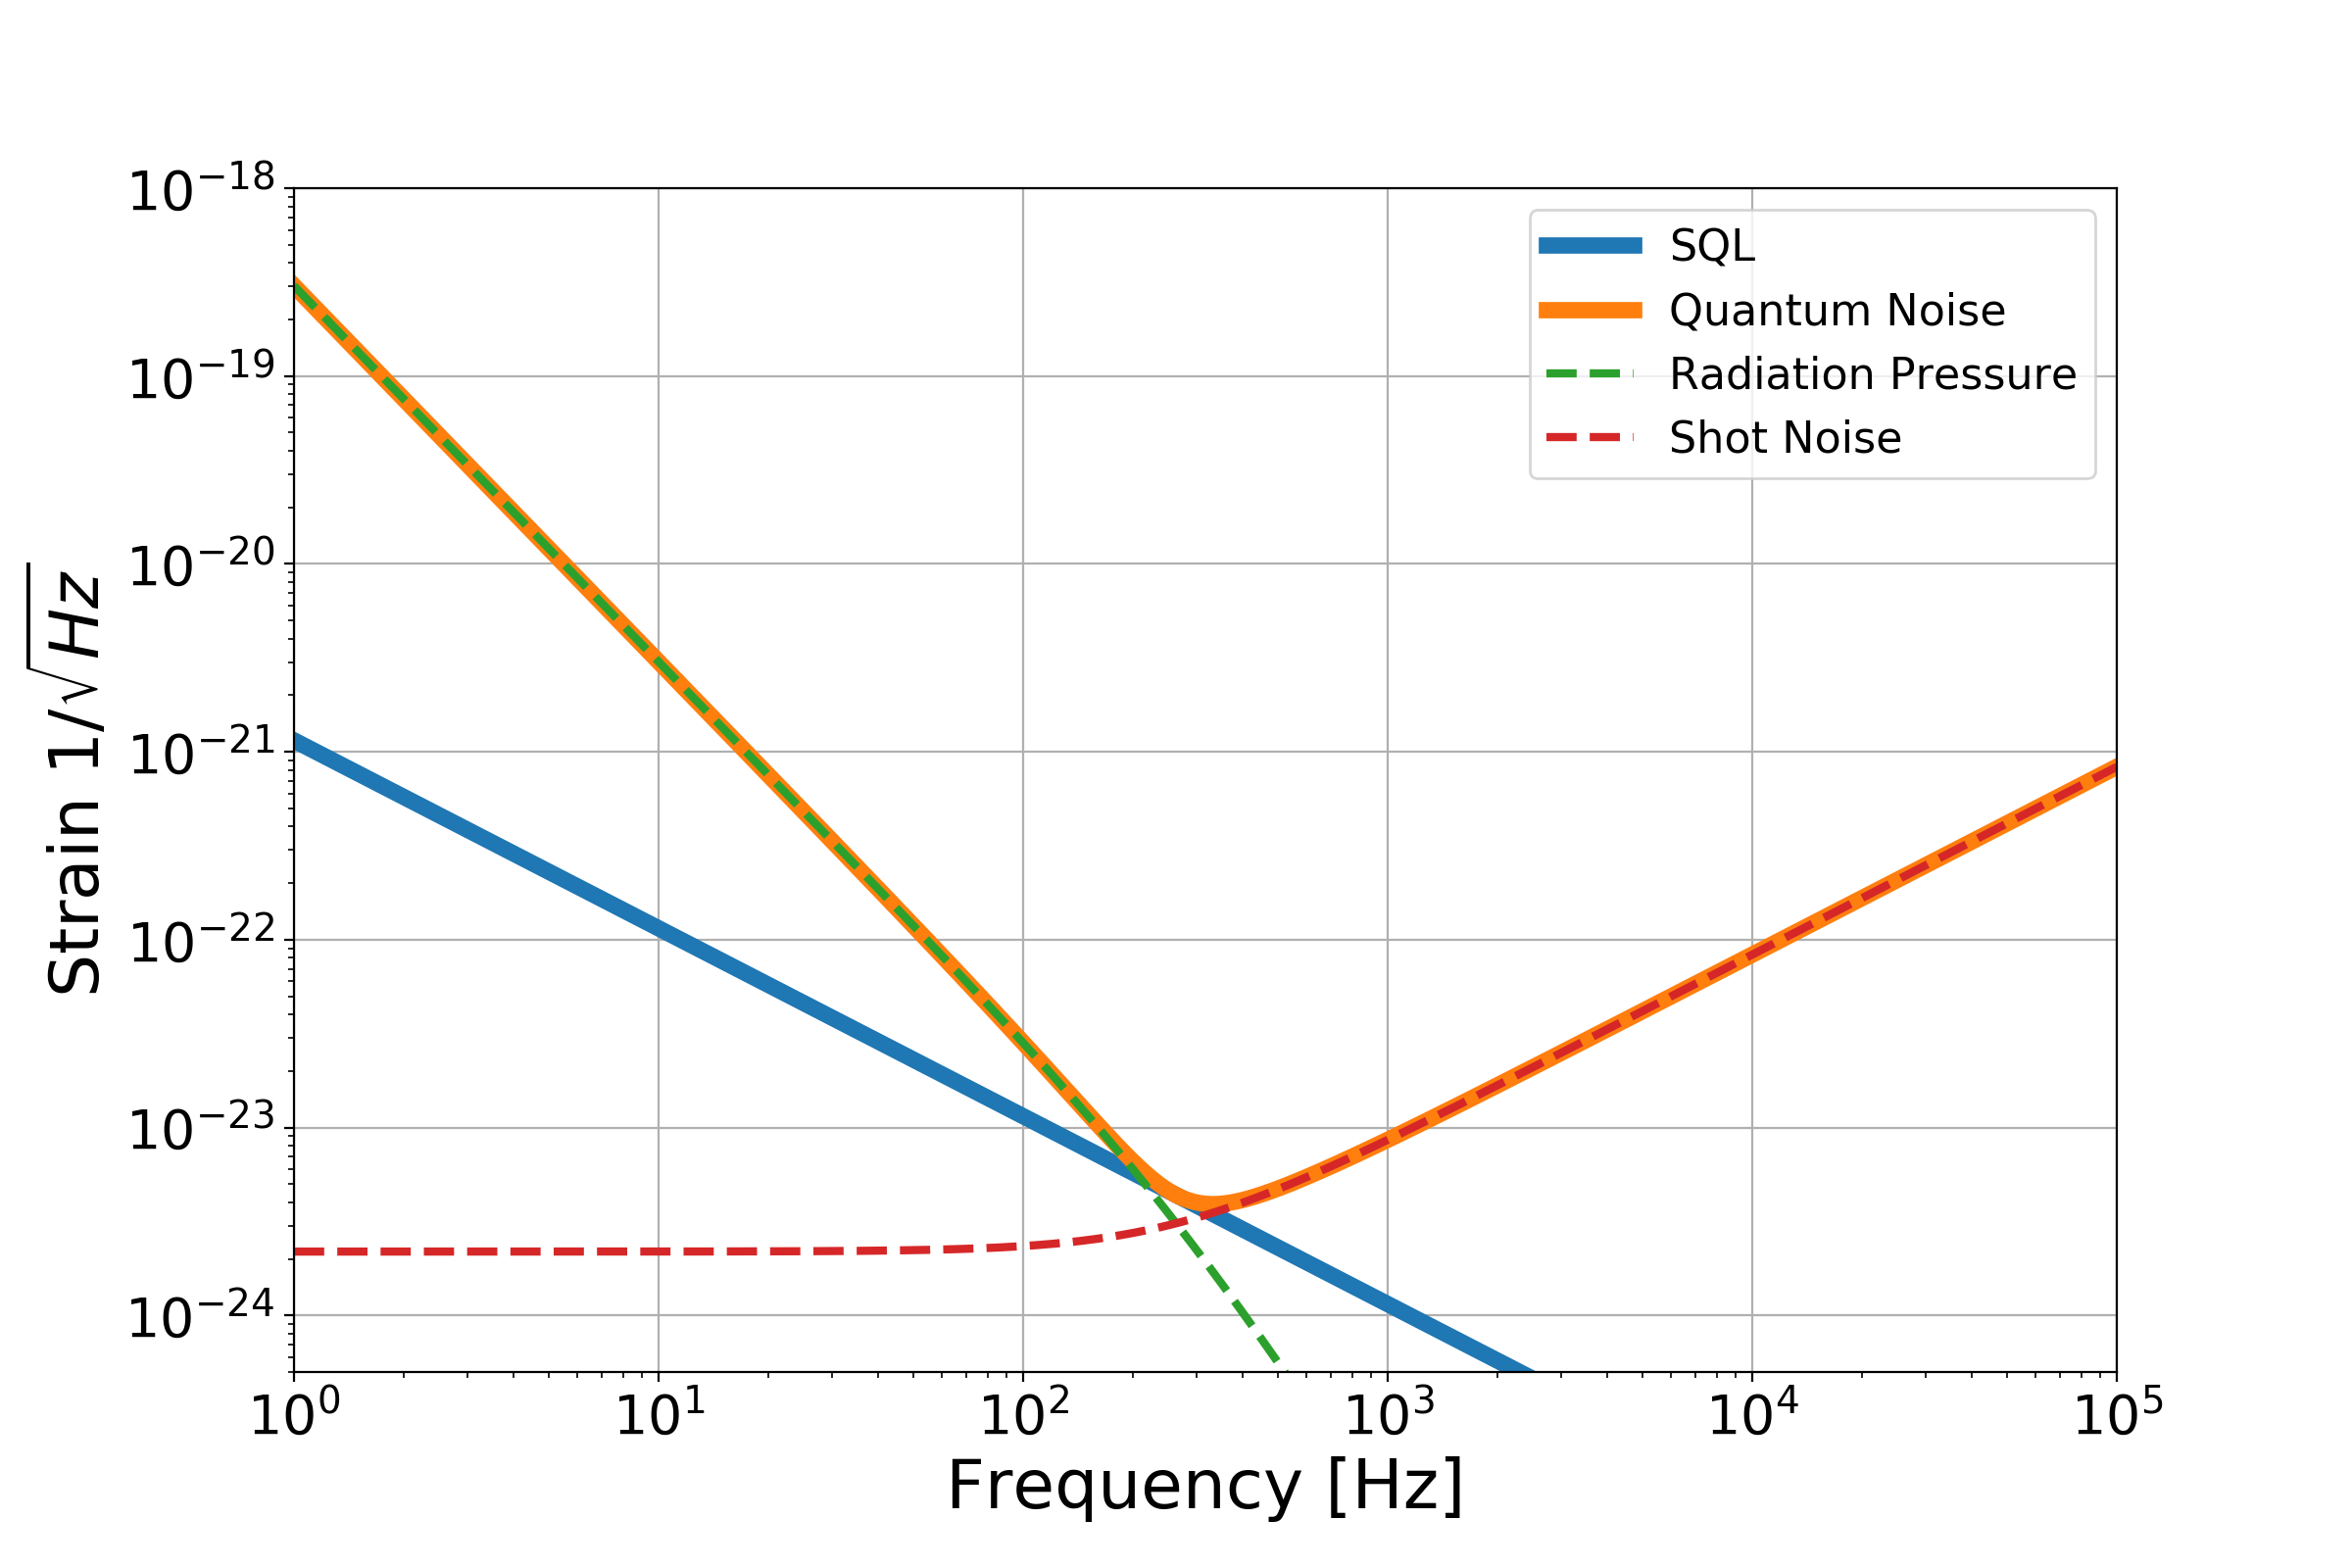
\includegraphics[width=\textwidth]{../Figures/Kimble_PRFPMI_QM.png}
			\caption{Power recycled Fabry Perot Michelson quantum noise}
			\label{fig:kimble_PRFMI}
		\end{subfigure}
		\hfill
		\begin{subfigure}[b]{0.5\textwidth}
			\centering
			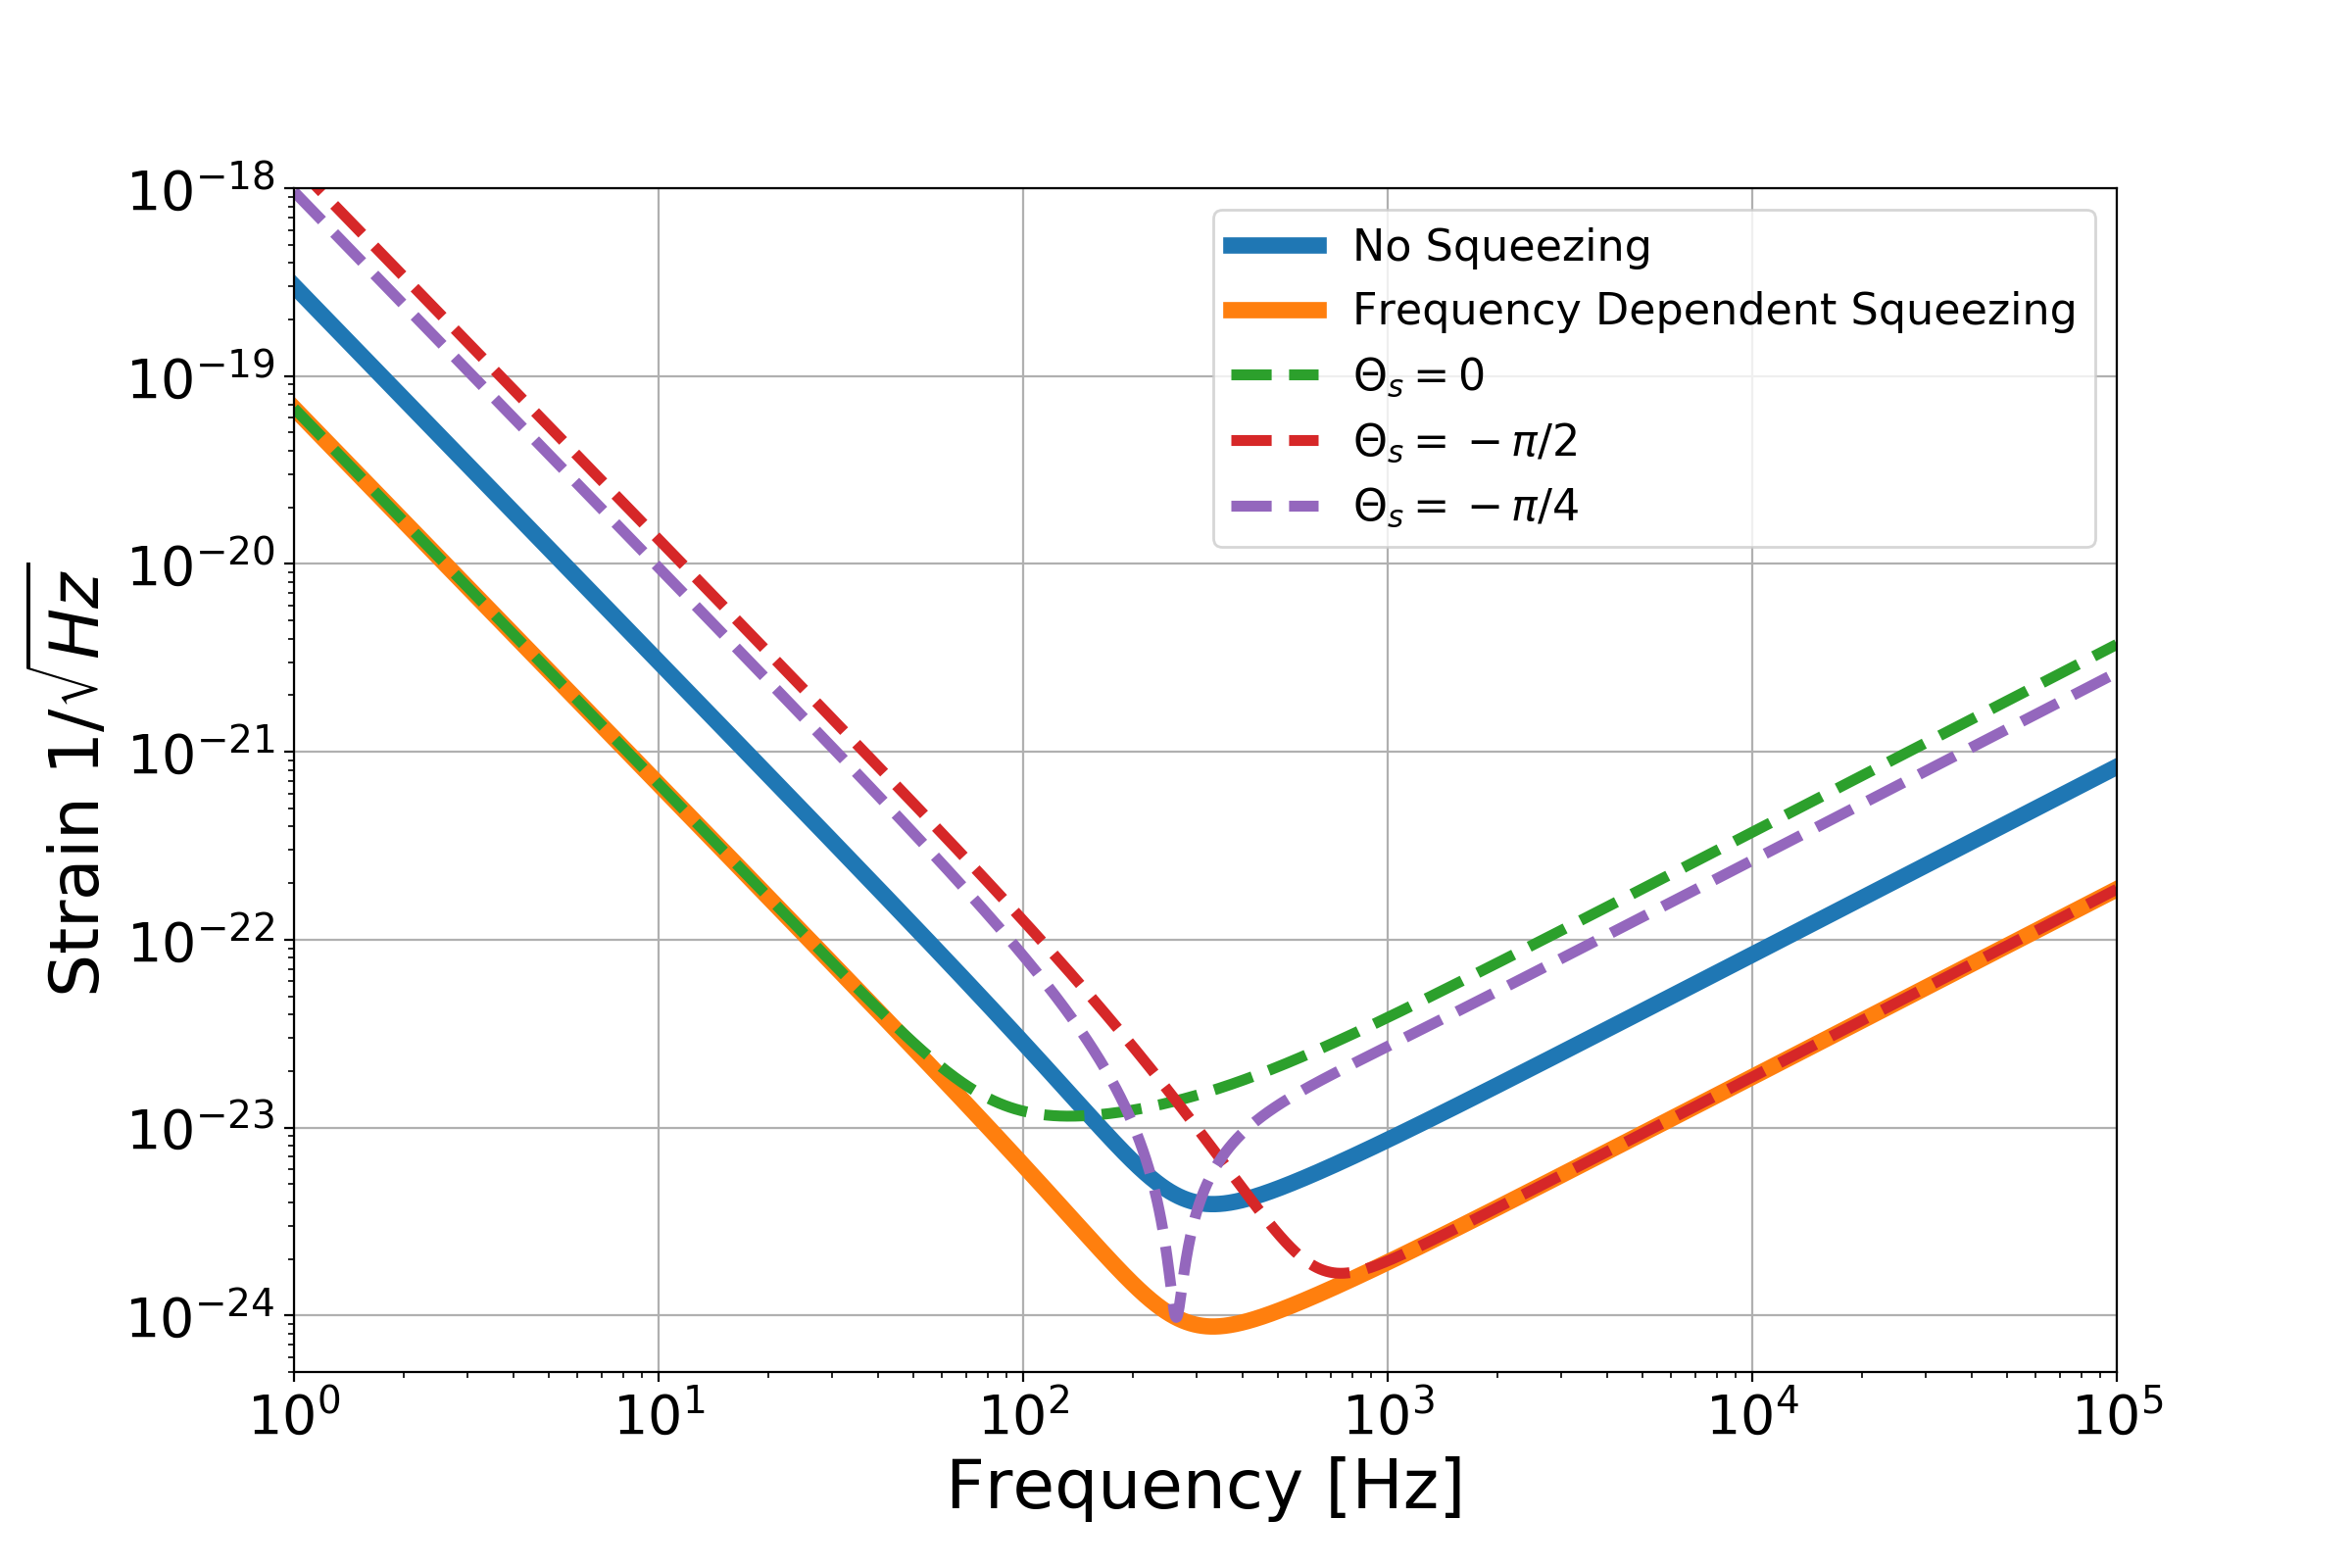
\includegraphics[width=\textwidth]{../Figures/Kimble_PRFPMI_QM_Sqz.png}
			\caption{Power recycled Fabry Perot Michelson quantum noise with various squeezing angles}
			\label{fig:kimble_PRFMI_sqz}
		\end{subfigure}
		\caption{Add a caption}
		\label{fig:PSD_PRFPMI}
	\end{figure}
\chapter{The Fundamentals of Mode-Matching}\label{chap:fund_mm}
		When dealing with the length sensing degrees of freedoms in Chapter \ref{LIGOInstrument}, the plane wave approximation is sufficient for describing the resonator dynamics. However, when trying to understand the misalignment and mode mismatch signals, it is necessary to incorporate Gaussian beams and their associated higher order modes. This formalism plays a pivotal role in the LIGO detectors because the gravitational wave is sensed using the fundamental eigenmode of the arm cavities and any coupling to higher order modes results in a loss of signal at the antisymmetric port.  Equally as important, the reduction of angular motion to remain locked relies on robust sensing of the cavity misalignment from external disturbances \cite{Fritschel_alignment} and torque-to-angle coupling \cite{SiggSidle}.  Mode matching is a second order effect but it will be shown in Chapter \ref{chapter:MM_LHO} that mismatches play an important role in the practical operation of a large scale interferometer.
			
		\section{Gaussian Beam Optics}
		To show that a Gaussian beam is a valid electromagnetic wave, consider the famous Maxwell's equations:
		\begin{equation}\label{eq:maxwell}
		\begin{aligned}
		 \nabla \times \mathbf{E} &=-\frac{\partial \mathbf{B}} {\partial t}
		\\\nabla \cdot \mathbf{B} &=0				
		\\\nabla \times \mathbf{B} &= \mu\ \mathbf{J} + \frac{1}{c^2} \frac{\partial \mathbf{E}} {\partial t}
		\\
		\nabla \cdot \mathbf{E} &= \frac{\rho}{\epsilon}
		\end{aligned}
		\end{equation}
		Concentrating on the electric field in vacuum, we arrive at the Helmholtz Equation
		\begin{equation}\label{Helmholtz}
		(\nabla^2 + k^2 ) \mathbf{U}(\mathbf{r},t) = 0
		\end{equation}
		where $k=\frac{2\pi\nu}{c}$ is the wave number and $\mathbf{U}(\mathbf{r},t)$ is the complex amplitude which can describe either the electric or magnetic fields.  There are a variety of solutions to equation \ref{Helmholtz} which include the plane and spherical waves \cite{Saleh}.  These two types of solutions are the extremes when considering the angle and spatial distribution as a function of propagation.  The plane wave which has been used in chapter \ref{intro} is a beam whose rays have no variance in the spatial direction as it propagates through space, whereas the spherical wave starts at a point and spreads as a function of distance from the origin. Somewhere in between these two extrema is the paraxial wave which is a wave pattern that consists of rays at small angles relative to the direction of propagation.  It is possible to express the paraxial solution to equation \ref{Helmholtz} as a plane wave with a modulated complex envelope $\mathbf{A}(r)$,
		\begin{equation}
		\mathbf{U}(\mathbf{r}) = \mathbf{A}(\mathbf{r}) e^{-ikz}
		\end{equation}
		However, in order for the paraxial wave to exist, $\mathbf{U}(r)$ must satisfy the Helmholtz equation. Alternatively, the $\mathbf{A}(r)$ must satisfy a separate differential equation known as the paraxial Helmholtz Equation which can be derived explicitly by imposing constraints that force the envelope to vary slowly with respect to the z-axis within the distance of one wavelength $\lambda = 2\pi/k$:

		\begin{subequations}
		\begin{equation}\label{paraxiala}
		\bigg| { \frac{\partial^2 \mathbf{A}}{\partial z^2} } \bigg|  \ll  \bigg| { k {\frac{\partial\mathbf{A}}{{\partial z}} } } \bigg|
		\end{equation}
		\begin{equation}\label{paraxialb}
		\bigg| { \frac{\partial^2 \mathbf{A}}{\partial z^2} } \bigg|  \ll  \bigg| { k {\frac{\partial^2 \mathbf{A}}{\partial x^2}} } \bigg|
		\end{equation}
		\begin{equation}\label{paraxialc}
		\bigg| { \frac{\partial^2 \mathbf{A}}{\partial z^2} } \bigg|  \ll  \bigg| { k{\frac{\partial^2 \mathbf{A}}{\partial y^2}}} \bigg|
		\end{equation}
		\end{subequations}
		The partial differential equation which arises is called the Paraxial Helmholtz Equation:
		
		\begin{equation}\label{paraHelmholtz}
		\nabla_T^2 A(r) - i2k \frac{\partial A(r)}{\partial z} = 0
		\end{equation}
		
		where $\nabla_T^2 = \frac{\partial^2}{\partial x^2} + \frac{\partial^2}{\partial y^2} $ is the transverse Laplacian.  A simple solution for equation \ref{paraHelmholtz} is the complex paraboloidal wave,
		
		\begin{equation} \label{complexenvelope}
		A(\mathbf{r}) = \frac{A_0}{q(z)} e^{\frac{-ikr^2}{2q(z)}} , \quad q(z)=z+iz_0
		\end{equation}
		
		The parameter $z_0$ is referred to as the Rayleigh range and is directly proportional to the waist size squared.  In order to separate the amplitude and phase portions of the wave, it is useful to rewrite $q(z)$ as
		
		\begin{equation}\label{invq}
		\frac{1}{q(z)} = \frac{1}{R(z)} - i \frac{\lambda}{\pi W^2(z)}
		\end{equation} 
		
		Plugging equation \ref{invq} into \ref{complexenvelope} leads directly to the complex amplitude for a Gaussian Beam
		\begin{equation}
		U(r,z) = A_0 \frac{W_0}{W(z)} e^{-\frac{r^2}{W^2(z)}} e^{-ikz - ik \frac{r^2}{2R(z)} + i \zeta(z)}
		\end{equation}
		where
		\begin{subequations}
		\begin{equation}
		W(z) = W_0 \sqrt{1 + \bigg( \frac{z}{z_0} \bigg)^2}
		\end{equation}
		\begin{equation}\label{ROC}
		R(z) = z \bigg[ 1 + \bigg( \frac{z}{z_0} \bigg)^2 \bigg]
		\end{equation}
		\begin{equation}\label{gouy}
		\zeta(z)= \text{tan}^{-1}\bigg(\frac{z_0}{z}\bigg)
		\end{equation}
		\begin{equation}
		W_0 = \sqrt{\frac{\lambda z_0}{\pi}}
		\end{equation}
		\end{subequations}\label{eq:gauss_params}
	
		The Gaussian beams are named as such because of the intensity distribution,
		\begin{equation}
		I(r,z) = \vert U(r,z) |^2 = I_0 \bigg[ \frac{w_0}{w(z)}\bigg]^2 \exp \bigg[ \frac{-2 r^2}{w^2(z)}\bigg]
		\end{equation}
		where $I_0 = \vert A_0\vert^2$ and has a peak at $r=0$ and $z=0$.  The width increases as the beam propagates along the $\hat{z}$ axis away from the waist position and the intensity maximum on the beam axis decreases (see Figure \ref{fig:GaussIntensity}),
		\begin{equation}
		I(0,z) = \frac{I_0}{1 + (z/z_0)^2}
		\end{equation}
		
		\begin{figure}[ht]
			\centering
			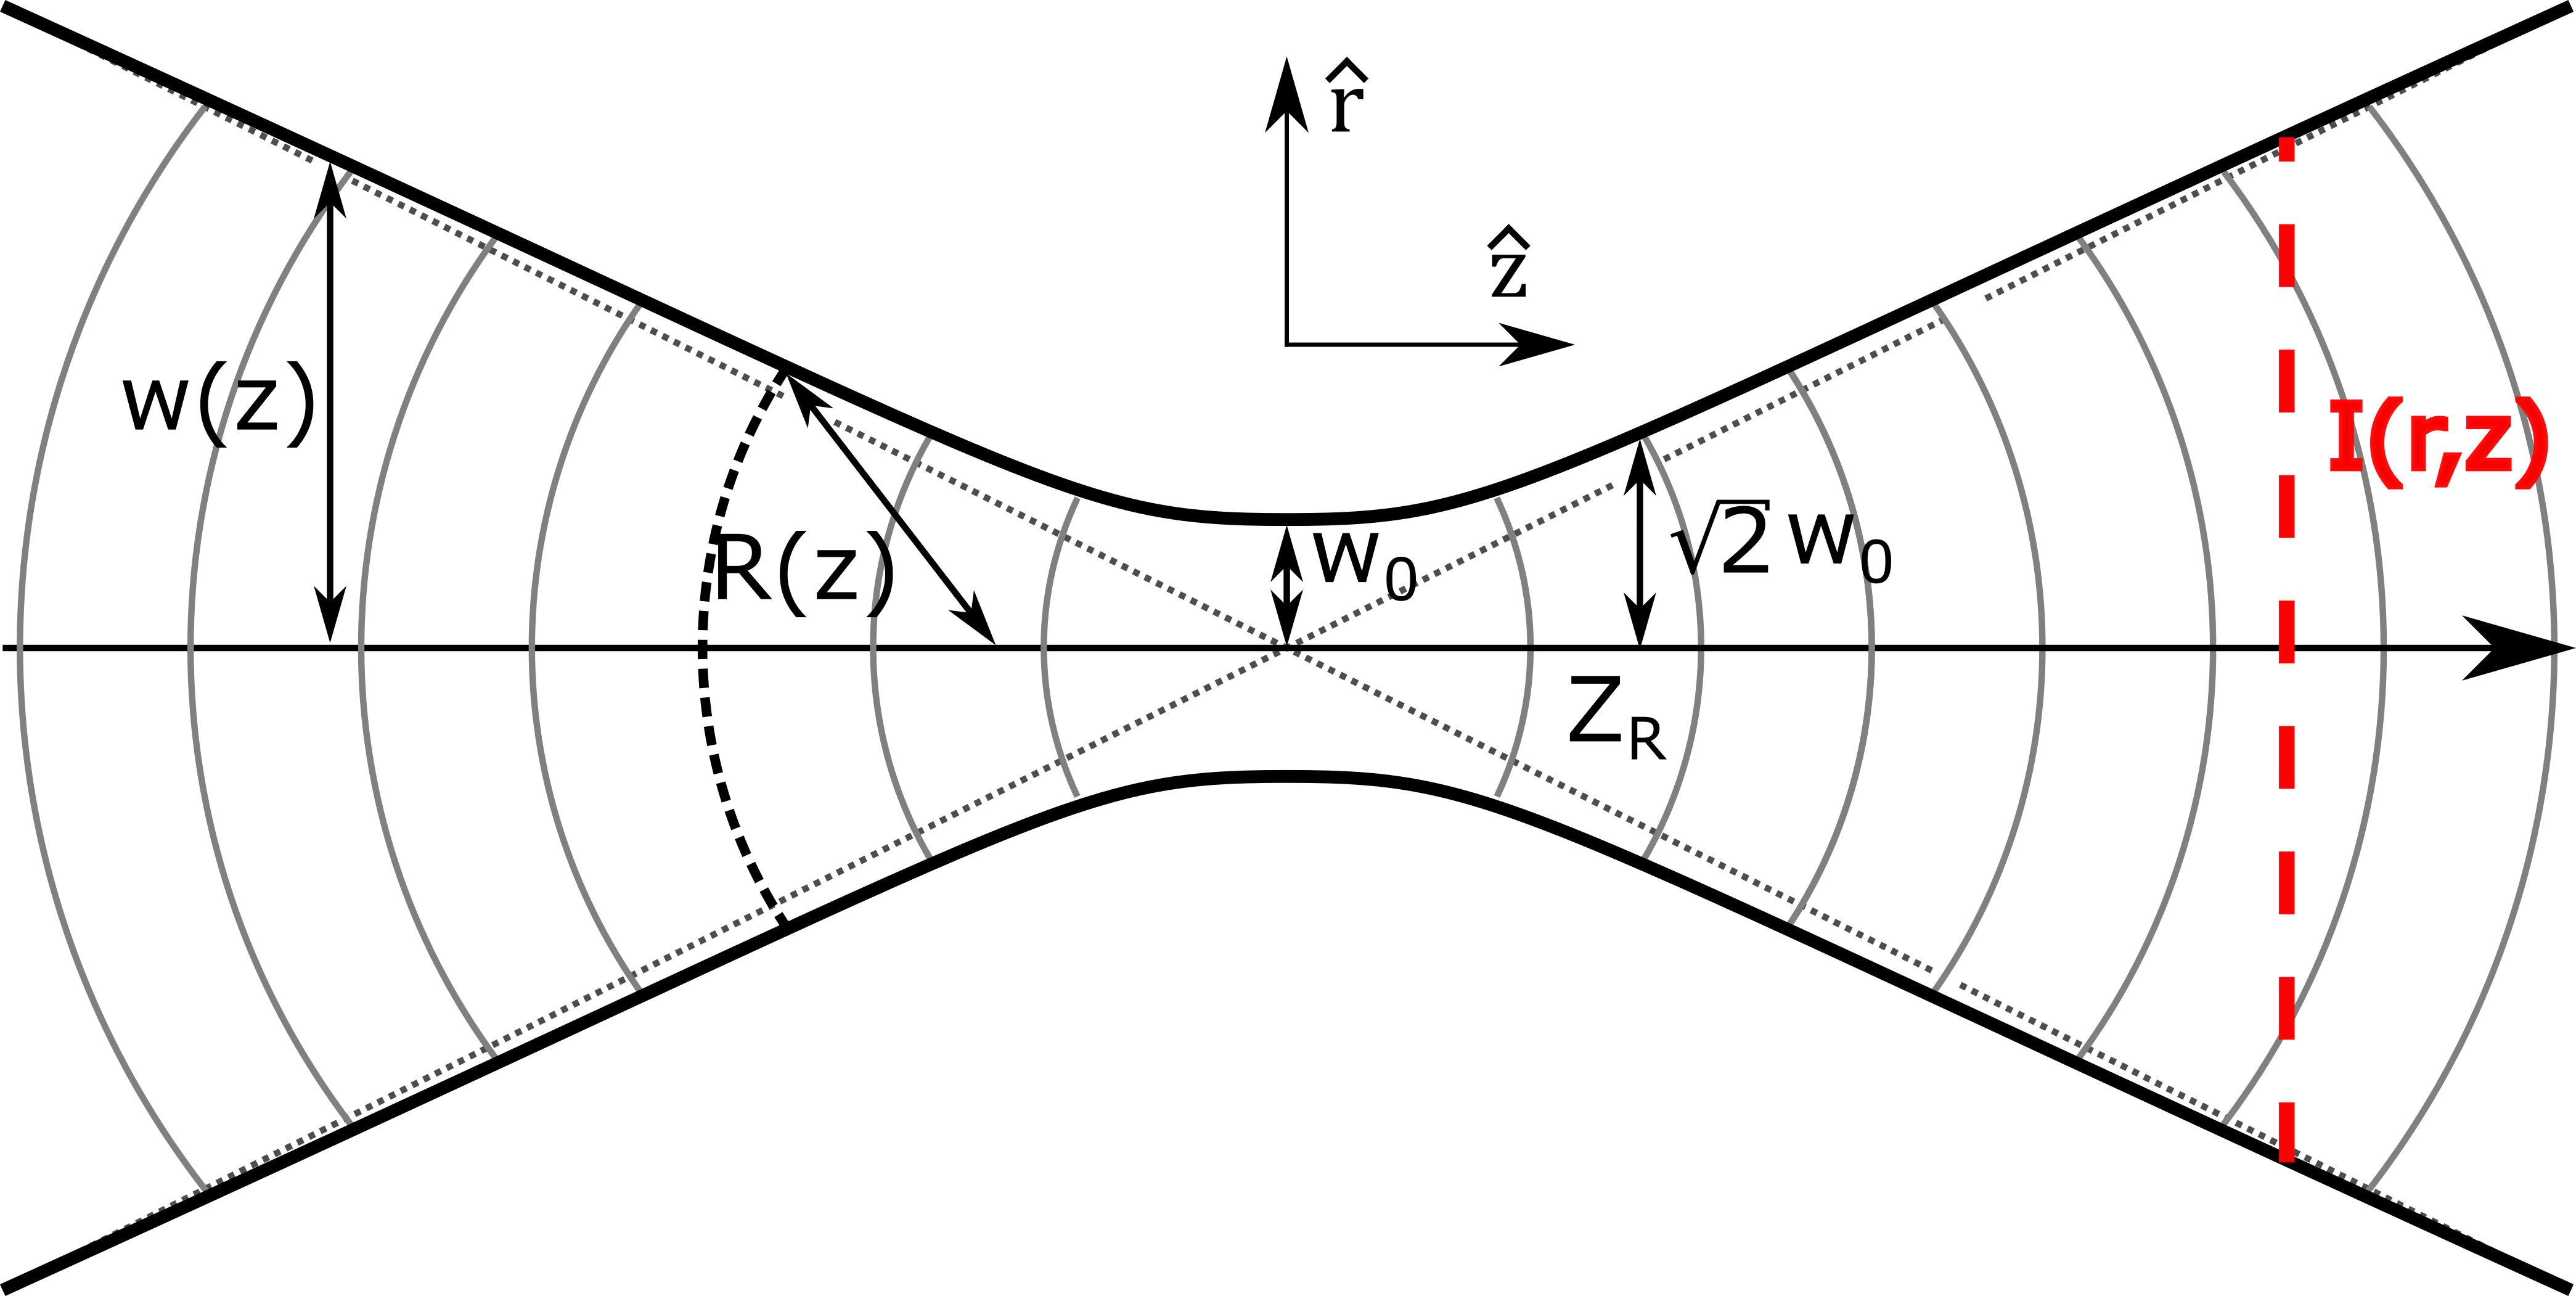
\includegraphics[width=0.65 \textwidth]{../Figures/GaussProfile.png}
			\caption[A depiction of the Gaussian beam properties with respect to cylindrical coordinates.]
			{\textbf{A depiction of the Gaussian beam properties with respect to cylindrical coordinates.} Because the beam is axially symmetric, the two coordinates are denoted by $\hat{r}$ for the radial and $\hat{z}$ for the axis of propagation with the origin located at the center. The thick dark lines represent the beam size, $w(z)$, which is minimal at the waist, $w(z)=w_0$ when $z=0$ and asymptotic towards $\lambda/\pi w_0$ when $z \approx \inf$ as shown by the dotted gray lines. The red dashed line represents the intensity cross section of the beam which changes to a wider and flatter profile as a function of distance from the waist.}
			\label{fig:GaussProfile}
		\end{figure}
	
		\begin{figure}[ht]
			\centering
			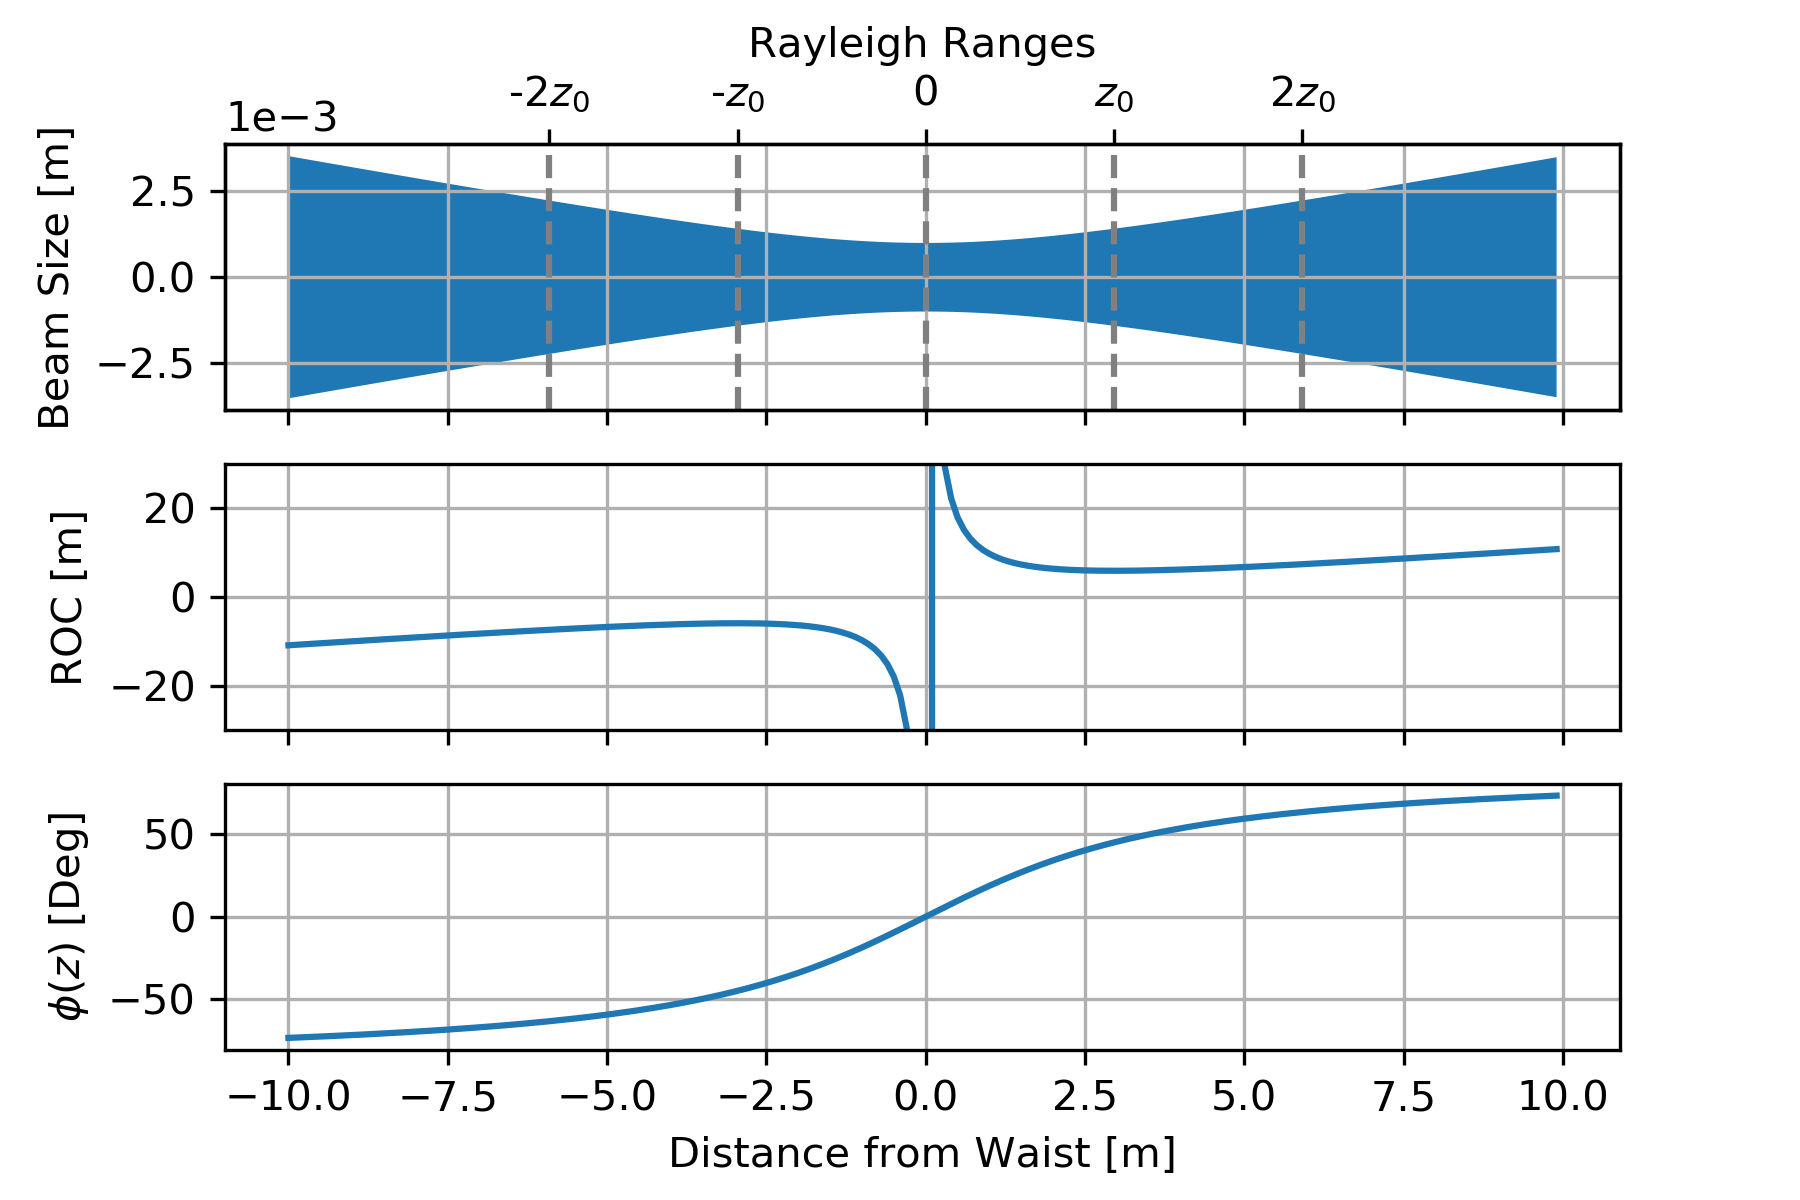
\includegraphics[width=0.6 \textwidth]{../Figures/GaussBeamParams.png}
			\caption[Beam size, radius of curvature, and Gouy phase as a function of distance propagation from the waist.] 
			{\textbf{Beam size, radius of curvature, and Gouy phase as a function of distance propagation from the waist.} The vertical dashed gray lines represent the integer number of Rayleigh ranges.  At the point $z=z_0$, the beam size is $\sqrt{2}$ of the waist size and the radius of curvature is minimal.  At this point, the Gouy phase propagation is lagging the plane wave by $\pi /4$ and the beam intensity is half of that at the waist.}
			\label{fig:GaussParams}
		\end{figure}

		\begin{figure}[ht]
			\centering
			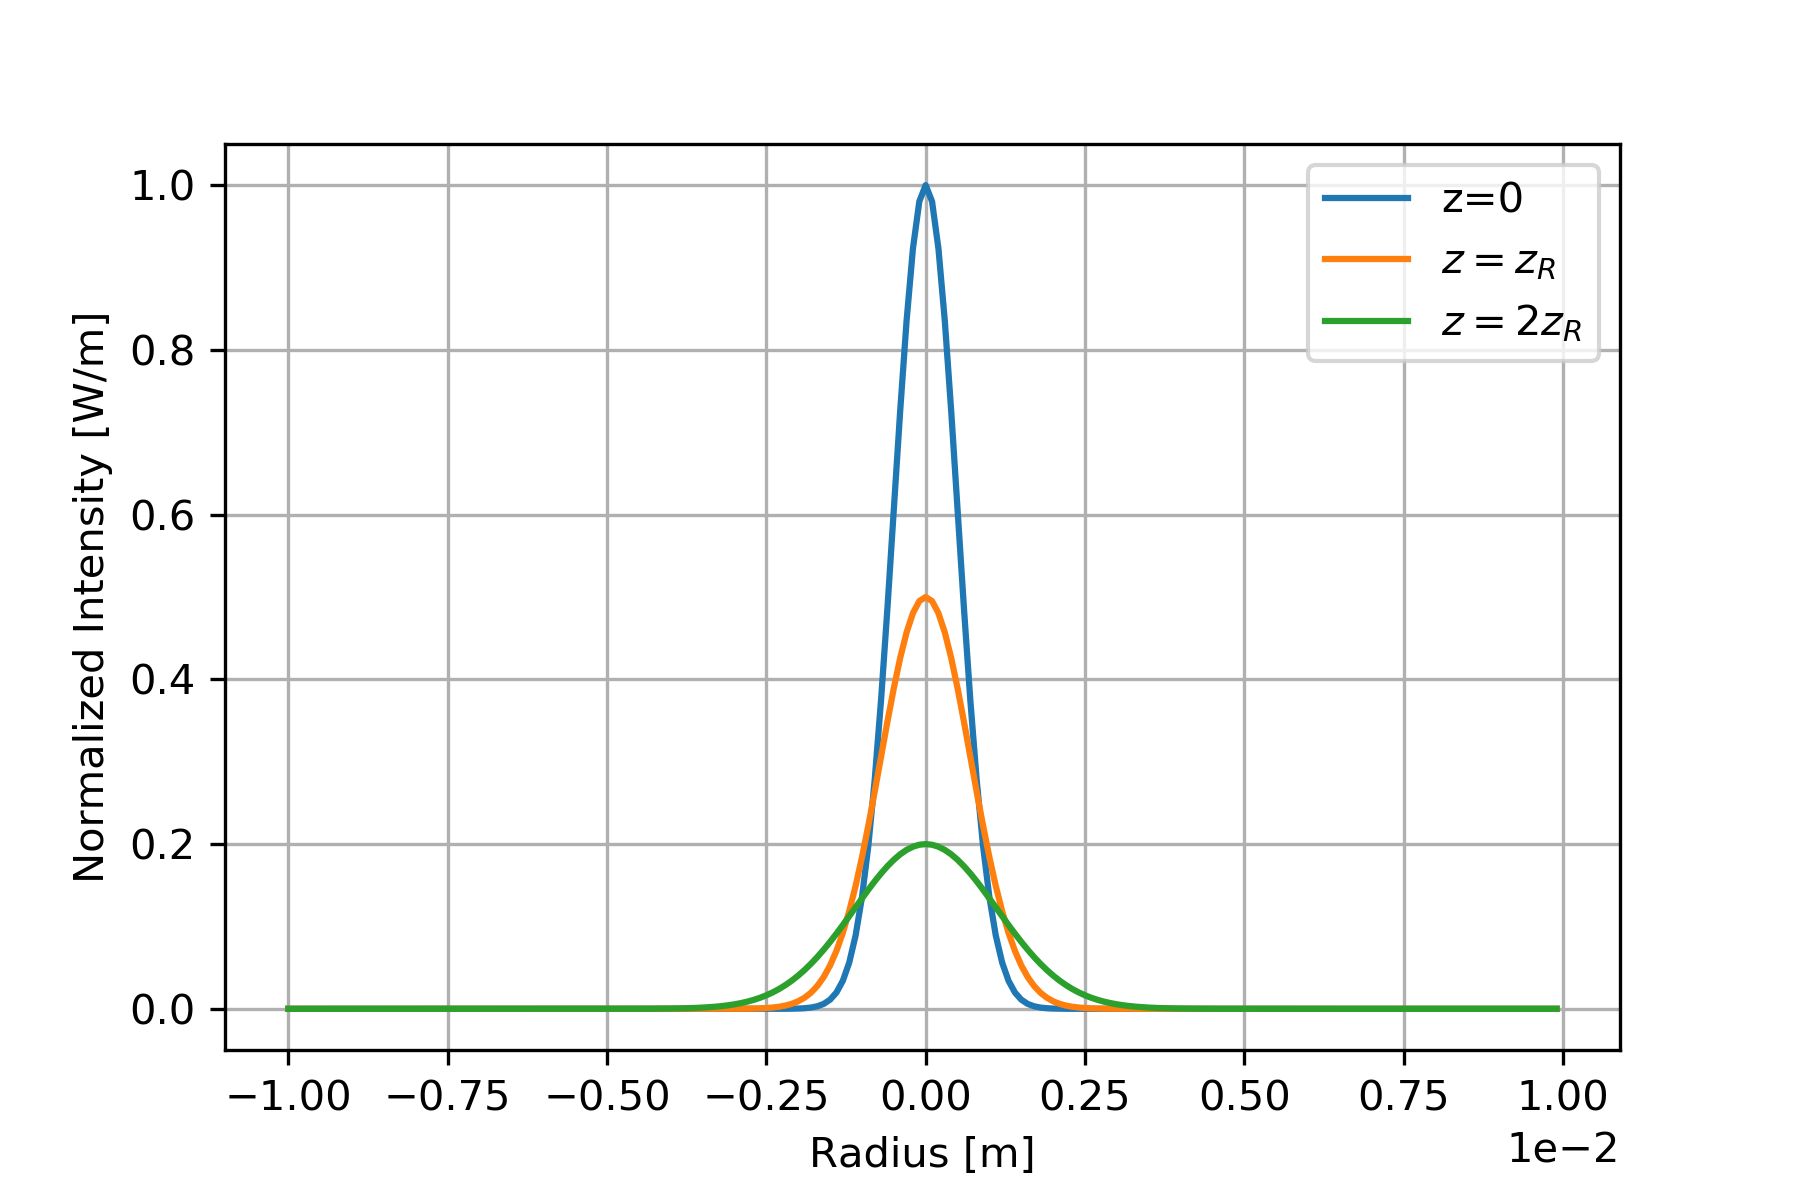
\includegraphics[width=0.65 \textwidth]{../Figures/GaussBeamIntensity.png}
			\caption{Intensity}
			\label{fig:GaussIntensity}
		\end{figure}
		
		\textbf{Hermite-Gauss Modes}
		
		The fundamental Gaussian beam is not the only solution which can be used to solve equation \ref{paraHelmholtz}.  In fact, there exists a complete set of solutions that can solve the paraxial Helmholtz Equation in rectangular coordinates, which are referred to as the Hermite Gauss modes
		\begin{equation}\label{HG}
		\begin{aligned}
		&U_{mn}(x,y,z) = A_{mn}\bigg[ \frac{W_0}{W(z)} \bigg] \mathbb{G}_m\Bigg( \frac{\sqrt{2}x}{W(z)}  \Bigg) \mathbb{G}_n\Bigg( \frac{\sqrt{2}y}{W(z)} \Bigg)\\
		&\times \text{exp} \bigg\{ -ikz - \frac{ik(x^2+y^2)}{2R(z)} + i(m+n+1)\zeta(z) \bigg\}
		\end{aligned}
		\end{equation}
		where,
		\begin{equation}
		\mathbb{G}(u) = \mathbb{H}(u) \, \text{exp}(-u^2/2)
		\end{equation}
		and $ \mathbb{H}(u)$ are the well known Hermite polynomials.  It is important to mention that the Gouy phase of the complex amplitude is different than the fundamental Gaussian beam by a factor of $(m + n + 1)$ and that the intensity distribution of these higher order modes are much different. Both of these facts will become extremely important in the following wavefront sensing discussion.
	
		\textbf{Laguerre Modes}
		
		Another complete set of alternative solutions to equation \ref{paraHelmholtz} exists which are called the Laguerre-Gauss modes
		
		\begin{equation}\label{LG}
		\begin{aligned}
		&V_{\mu\nu}(\rho,\theta,z) = A_{\mu\nu}\bigg[ \frac{W_0}{W(z)} \bigg] \mathbb{L}^{\mu}_{\nu} \Bigg( \frac{\sqrt{2}x}{W(z)}  \Bigg) \\
		&\times \text{exp} \bigg\{-ikz-\frac{ik\rho^2}{2R(z)} + i(\mu+2\nu+1)\zeta(z) \bigg\}
		\end{aligned}
		\end{equation}
		
		where $\mathbb{L}^{\mu}_{\nu} \Big( \frac{\sqrt{2}x}{W(z)}  \Big)$ is the Laguerre polynomial function. Both equations \ref{HG} and \ref{LG} are able to fully describe any complex electromagnetic amplitude; and because they both form complete sets, there is a rotation which can map from one basis to the other \cite{BEIJERSBERGEN} \cite{ONeilModeTransform}
		
		\begin{equation}
		U^{LG}_{\mu \nu} (x,y,z) = \sum\limits_{k}^{N} i^k b(n,m,k) U^{HG}_{N-k,k} (x,y,z)
		\end{equation}
		where
		\begin{equation}
		b(n,m,k) = \sqrt{\bigg( \frac{(N-k)!k!}{2^N n!m!} \bigg)} \frac{1}{k!} \frac{\text{d}^k}{\text{d}t^k}[(1-t)^m (1+t)^m]\vert_{t=0}
		\end{equation}

		\subsection{Misalignment and Higher Order Modes}\label{Misalign}
		Morrison and Anderson \cite{Anderson} \cite{Morrison} derived a simplistic way of how small misalignments and mode mismatch in cavities can couple the fundamental Gaussian beam into various higher order modes.  This is done by taking a linear cavity and using its perfectly matched Gaussian beam as a reference, and then varying the input electric field with small perturbations and expanding in terms of the higher order modes.  So long as the mismatches are small, it is possible to consider only the first few terms of the expansion which have gained most of their power from the fundamental mode.  Between various texts, the terms misalignment and mode mismatch are used interchangeably, which is not incorrect but creates some confusion.  This thesis will try to distinguish the two effects because the actuators and sensors used for correction can be quite different.
		
		Consider the first three Hermite-Gauss modes of equation \ref{HG} in one dimension and normalized to set the total optical power to unity:
		\begin{equation}
		\label{Gauss1D}
		\begin{aligned}
				U_{0}(r) & =	\bigg( \frac{2}{\pi w^2(z)} \bigg)^{1/4}  e^{-r^2/w^2(z)}		&
		\\		U_{1}(r) &	=	\bigg( \frac{2}{\pi w^2(z)} \bigg)^{1/4}  \frac{2r}{w(z)} \quad e^{-r^2/w^2(z)}&,
		\\	 	U_{2}(r) &	=	\bigg( \frac{2}{\pi w^2(z)} \bigg)^{1/4}  \frac{1}{\sqrt{2}} \bigg( \frac{4r^2}{w^2(z)} - 1 \bigg)   e^{-r^2/w^2(z)}
		\end{aligned}
		\end{equation}
		
		\subsubsection{Beam Axis Tilted}
		If the input beam entering an optical cavity is tilted by an angle $\alpha$ with respect to the nominal cavity axis, the wave front of the input beam will have an extra phase propagation relative to the cavity that is approximately proportional to $e^{ik \alpha r}$.  By implementing the small angle approximation, which is valid if the misalignment is much smaller than the divergence angle of the fundamental mode $k \alpha r << 1$, the resultant input beam is
		\begin{equation}
		\Psi \approx U_{0}(r) e^{ik \alpha r} \approx U_{0}(r) ( 1 + ik \alpha r ) =  U_{0}(r) + \frac{ik \alpha w(z)}{\sqrt{2\pi}} U_{1}(r)
		\end{equation}
		Here, the factor associated with the first higher order mode is complex, indicating there is a 90 degree phase difference between the fundamental and off-axis mode. 
		\subsubsection{Beam Axis Displaced}
		If the input beam is displaced in the transverse direction by a quantity $\Delta r$, the resultant waveform will be
		
		\begin{equation}
		\begin{aligned}
			\Psi 	&=  		U_{0}(r + \Delta r	) 
			\\		&= 			\bigg( \frac{2}{\pi w^2(z)} \bigg)^{1/4}  e^{-(r+\Delta r)^2/w^2(z)}
			\\		&= 			\bigg( \frac{2}{\pi w^2(z)} \bigg)^{1/4}  e^{-(r^2 + 2r \Delta r  + \Delta r^2)/w^2(z)}
			\\		&\approx 	\bigg( \frac{2}{\pi w^2(z)} \bigg)^{1/4}  e^{-r^2/w^2(z)} e^{-2r \Delta r/w^2(z)}
			\\		&\approx 	\bigg( \frac{2}{\pi w^2(z)} \bigg)^{1/4}  e^{-r^2/w^2(z)} \bigg(1 - \frac{2r \Delta r}{w^2(z)} \bigg)
			\\		&=			\bigg( U_0(r) - \sqrt{\frac{2}{\pi}} \frac{\Delta r }{w(z)} U_1(r)	 \bigg)
		\end{aligned}
		\end{equation} 
		Similar to a tilted input beam axis, the displaced beam axis couples power to the first higher order mode, however, the latter does not have a 90 degree phase difference.  This point is extremely important when trying to discern between the two effects.  Although comparing the two cases in Figure \ref{fig:BeamAxisRotated}, one can already see the difference between wavefronts in the near field, $z<<z_R$, and the far field, $z>>z_R$.  In the near field, there is no wavefront phase difference between the original beam and the displaced beam, but there is one for a tilted beam.  Conversely in the far field, there is no phase difference due to a tilted beam, but there is one from a displaced beam.  In order to implement a closed loop feedback system, the wavefront sensors discussed in Section \ref{WFS} will use this precise logic to extract an error signal.
		
		\subsection{Mode Mismatch and Higher Order Modes}\label{Modemismatch}
		Using the same formalism as above, determining the second order mode coupling from mode mismatch is repeated.
		
		\subsubsection{Waist Size Shifted}
		By considering the effect of evaluating the fundamental mode at the waist position, $z=0$, but changing the waist size by a small amount $\epsilon$, it is possible to see coupling into higher order modes by expanding to first order.	
		\begin{equation}
		\begin{aligned}
		\Psi 	&=  		U_{0} \big(r,w(z) = w_0/(1+\epsilon) \big) 
		\\		&= 			\bigg( \frac{2}{\pi w_0^2} \bigg)^{1/4} \sqrt{1 + \epsilon} \quad e^{-r^2 (1+\epsilon)^2/w_0^2 }
		\\		&\approx 	\bigg( \frac{2}{\pi w_0^2} \bigg)^{1/4} (1 + \epsilon /2) \quad e^{-r^2/w_0^2} \quad e^{-2r^2\epsilon/w_0^2} 
		\\		&\approx 	\bigg( \frac{2}{\pi w_0^2} \bigg)^{1/4} (1 + \epsilon /2) \quad e^{-r^2/w_0^2} \quad (1-2r^2\epsilon/w_0^2)
		\\		&\approx 	\bigg( \frac{2}{\pi w_0^2} \bigg)^{1/4} \bigg(1+ 2\epsilon\bigg(\frac{1}{4} - \frac{r^2}{w_0^2}\bigg) \bigg ) \quad e^{-r^2/w_0^2}	
		\\		&=			U_0(r) \, - \, \frac{\epsilon}{\sqrt{2}} \, U_2(r)
		\end{aligned}
		\end{equation}
		By changing the waist size by a small amount, the mismatch will couple the fundamental mode to the in-phase second order Hermite Gauss mode.
		
		\subsubsection{Waist Position Shifted}
		To repeat the process from above with a waist position shift, it is useful to start with a more general equation that includes the phase that is gained from including the radius of curvature,
		\begin{equation}\label{EFieldwPhase}
		\Psi = 	\bigg( \frac{2}{\pi w^2(z)} \bigg)^{1/4} \quad e^{-r^2/w^2(z)} \quad e^{-ikr^2/2R(z)}
		\end{equation}
		where $R(z)$ is from equation \ref{ROC}.  It is also useful to approximate the shift in waist position along the longitudinal axis is small compared to the Rayleigh range of the beam, $\Delta z << z_0$, which leaves the waist size approximately the same and the radius of curvature inversely proportional to the shift. 
		\begin{subequations}
		\begin{align}
		\begin{split}
			w^2(\Delta z)	&= 	w^2_0 \bigg[1 + \bigg(\frac{\Delta z}{z_0}  \bigg)^2 \bigg]  \approx	w^2_0
		\end{split}\\
		\begin{split}
			R(\Delta z) 	&=	\Delta z \bigg(1 + \bigg(\frac{z_0}{\Delta z}\bigg)^2\bigg) \approx	\frac{z_0^2}{\Delta z}
		\end{split}
		\end{align}
		\end{subequations}
	Plugging the equations above into \ref{EFieldwPhase},
		\begin{equation}
		\begin{aligned}
		\Psi 	&\approx	\bigg( \frac{2}{\pi w_0^2} \bigg)^{1/4} \quad e^{-r^2/w_0^2} \quad e^{-ikr^2 \Delta z /2 z_0^2}
		\\		&\approx	\bigg( \frac{2}{\pi w_0^2} \bigg)^{1/4} \quad e^{-r^2/w_0^2} \quad \bigg( 1-\frac{ikr^2 \Delta z}{2 z_0^2}  \bigg)
		\\		&=			U_0(r) - \bigg( \frac{2}{\pi w_0^2} \bigg)^{1/4} e^{-r^2/w_0^2} \quad \frac{ikr^2 \Delta z}{2 z_0^2}
		\\		&=			U_0(r) - i \frac{\Delta z}{2k w_0^2} \bigg( 4U_2(r) + U_0(r) \bigg)
		\end{aligned}
		\end{equation}
		The equations above show that a fundamental Gaussian mode that is shifted in waist position will couple power to the second order Hermite Gauss mode.  Although changes in the waist size or position couple power to the same mode, they differ by a 90 degrees in phase as denoted by the extra factor of $i$ in the coupling coefficient.  By recognizing the two effects are in different quadrature phases will allow a user to design a system to distinguish between the different types of physical couplings, this is shown in Section \ref{WFS}.
		
		 In order to be physically valid one would need to consider the full two dimensional space so that the equation would encapsulate the full transverse mode, however, the x and y components would follow the exact same derivation. On that point, it is important to note that only the mode mismatch couplings from either a varying waist position or size has higher order modes that are circularly symmetric.
		
		\begin{figure*}
			\centering
			\begin{subfigure}[b]{0.475\textwidth}
				\centering
				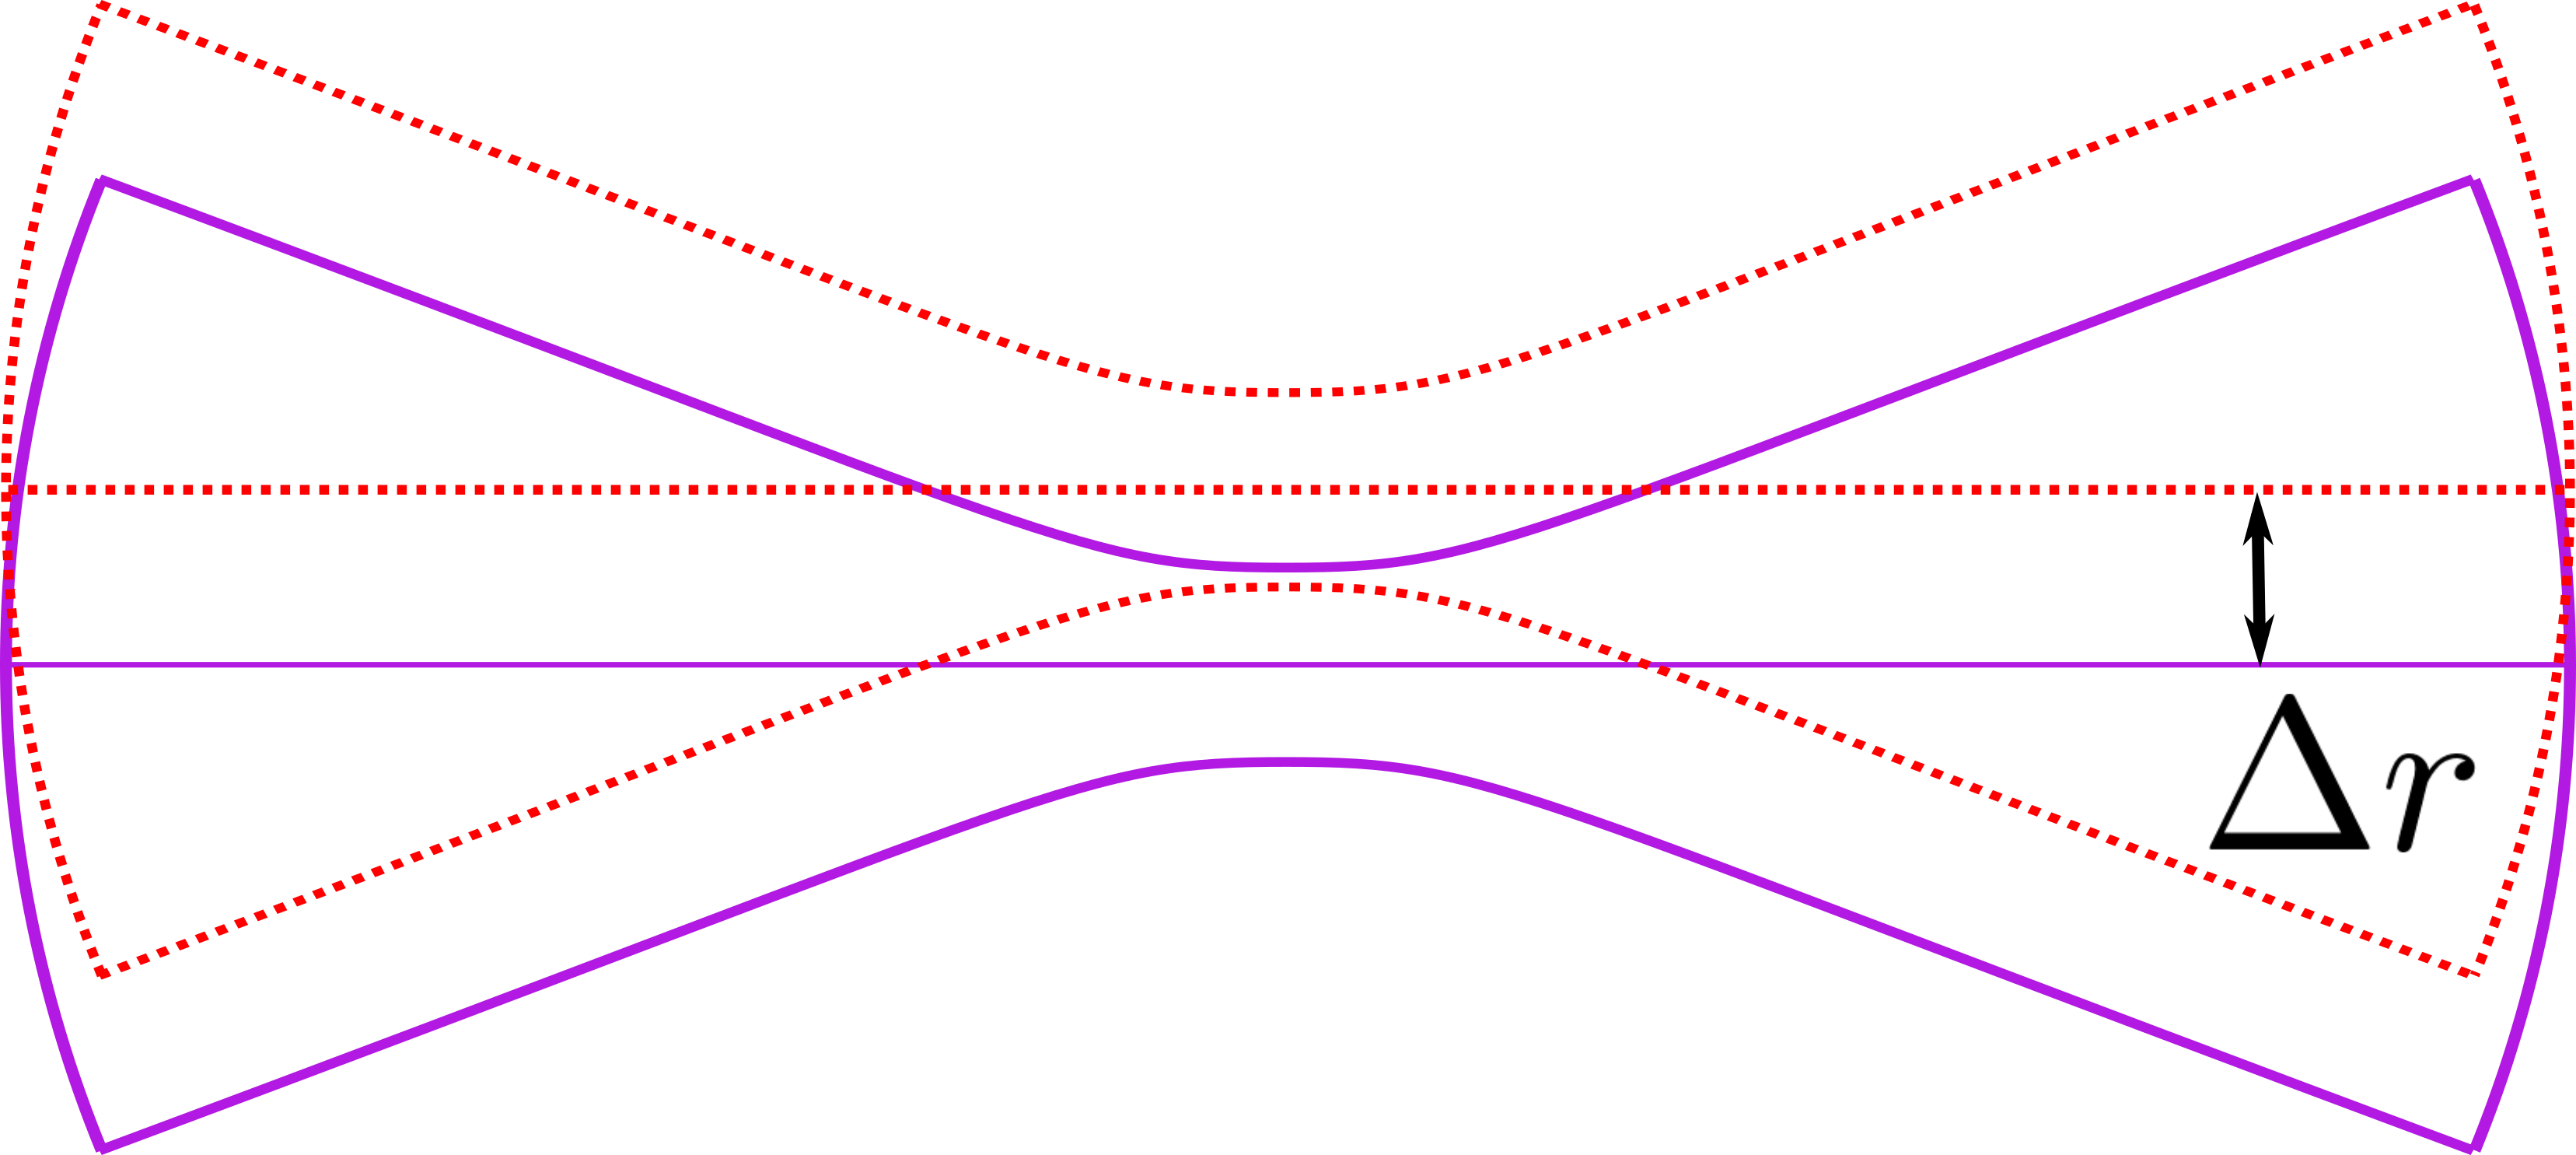
\includegraphics[width=\textwidth]{../Figures/BeamAxisDisplaced.png}
				\caption[]{\textbf{Beam axis displaced by $\Delta r$.}}    
				\label{fig:BeamAxisDisplaced}
			\end{subfigure}
			\hfill
			\begin{subfigure}[b]{0.475\textwidth}  
				\centering 
				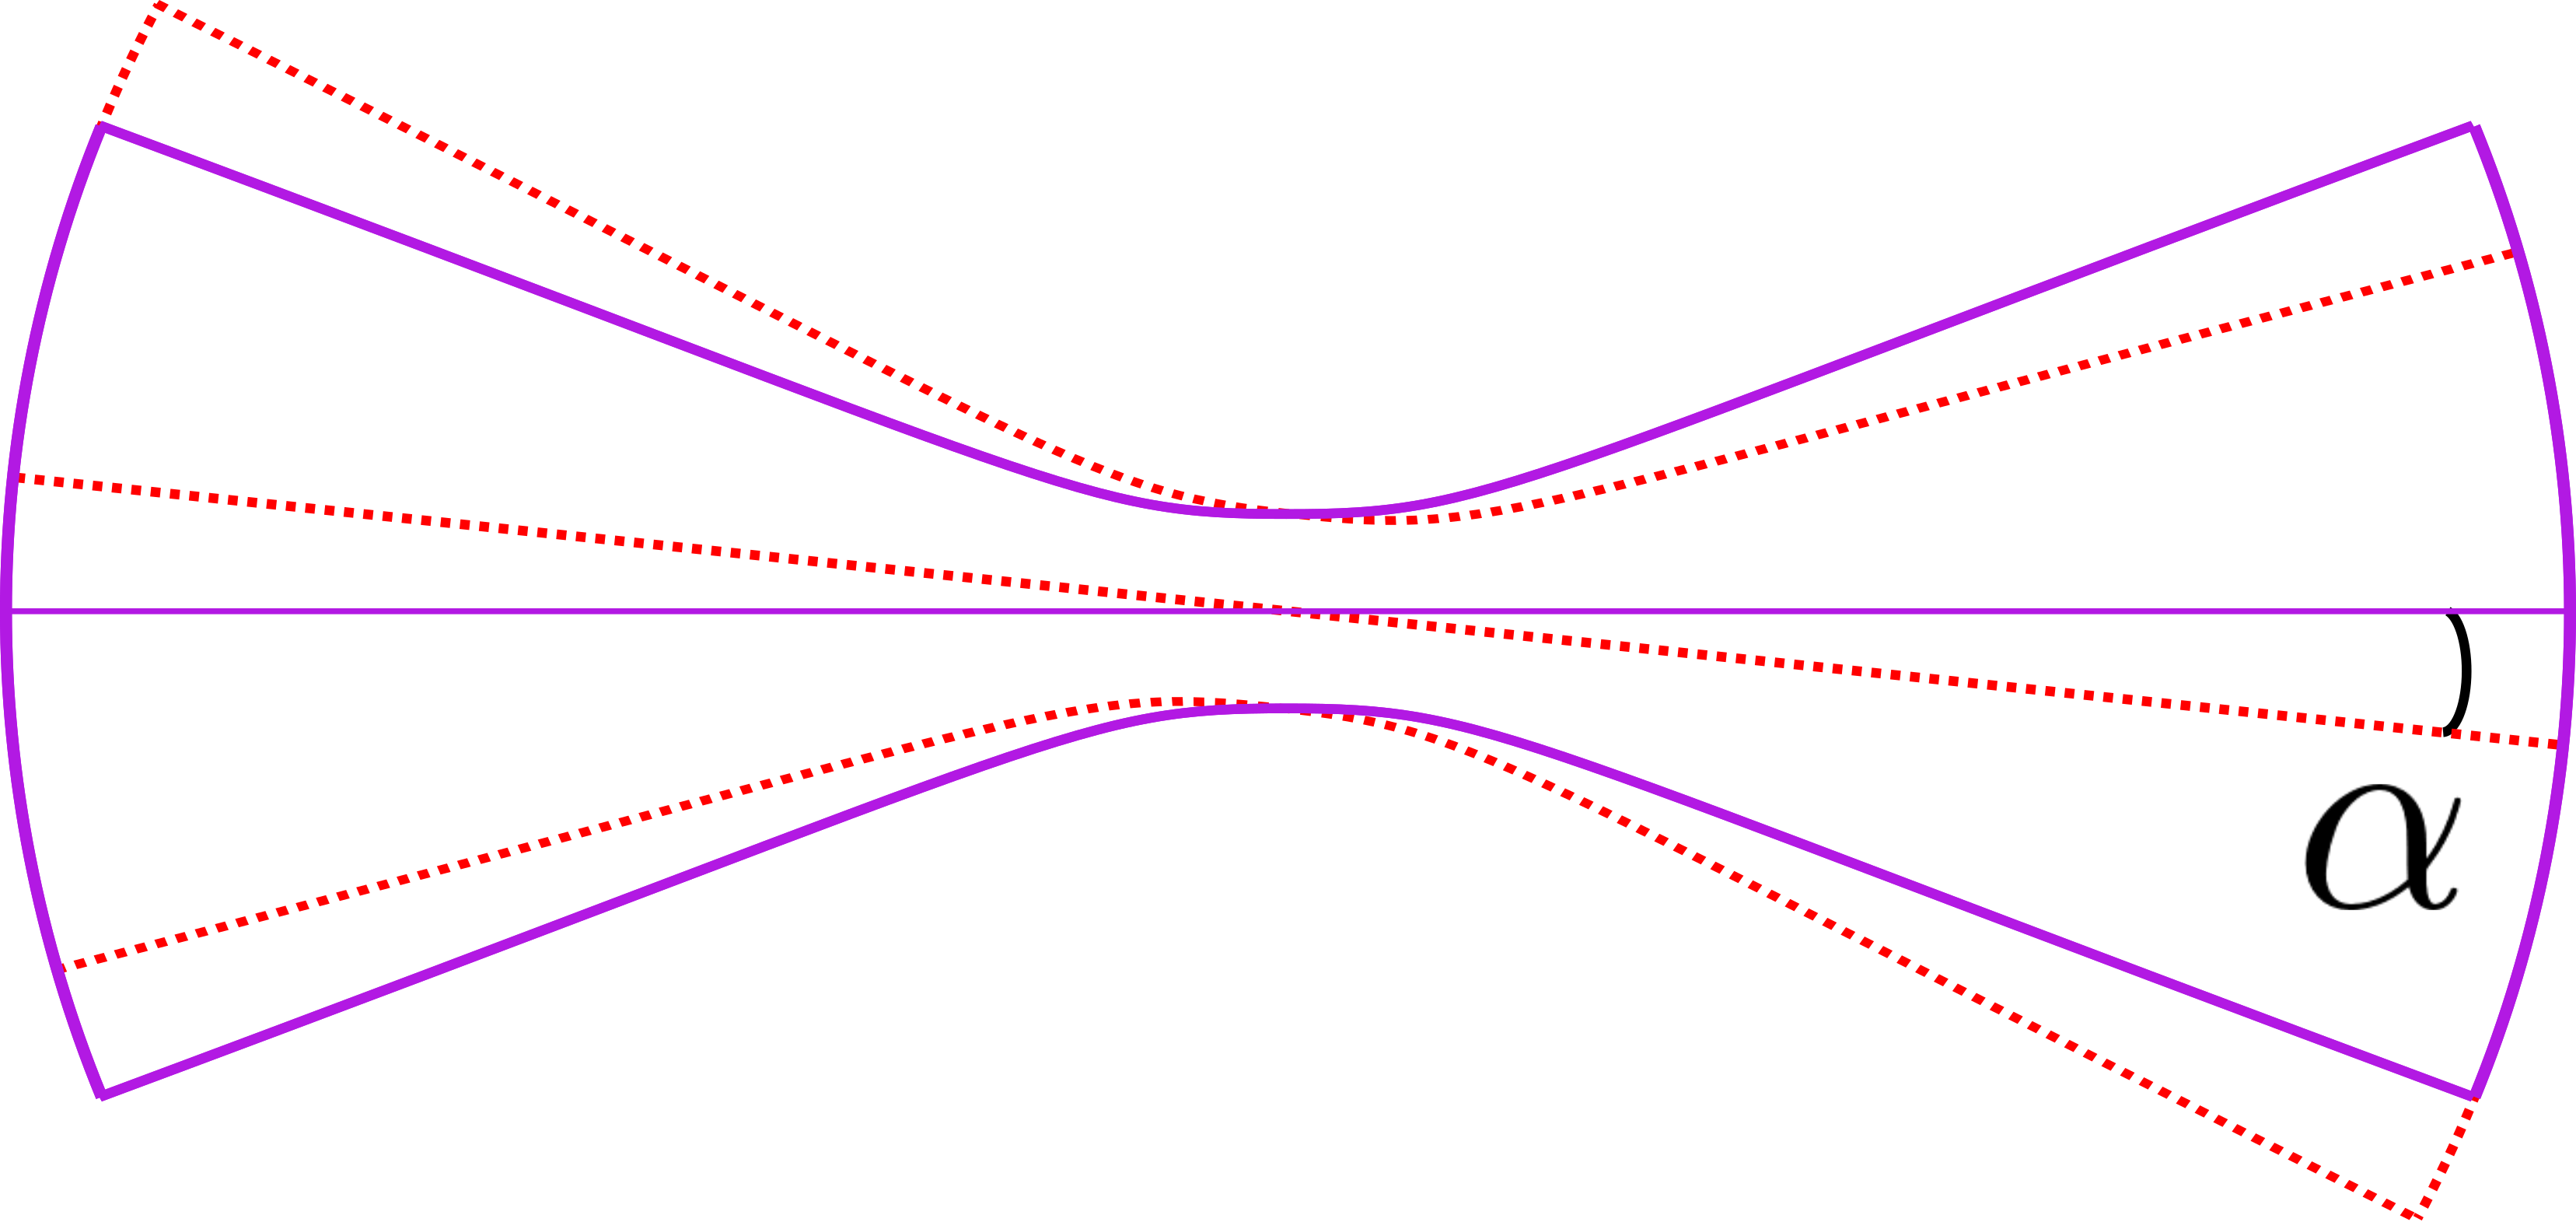
\includegraphics[width=\textwidth]{../Figures/BeamAxisRotated.png}
				\caption[]{\textbf{Beam axis rotated by $\alpha$.}}    
				\label{fig:BeamAxisRotated}
			\end{subfigure}
			\vskip\baselineskip
			\begin{subfigure}[b]{0.475\textwidth}   
				\centering 
				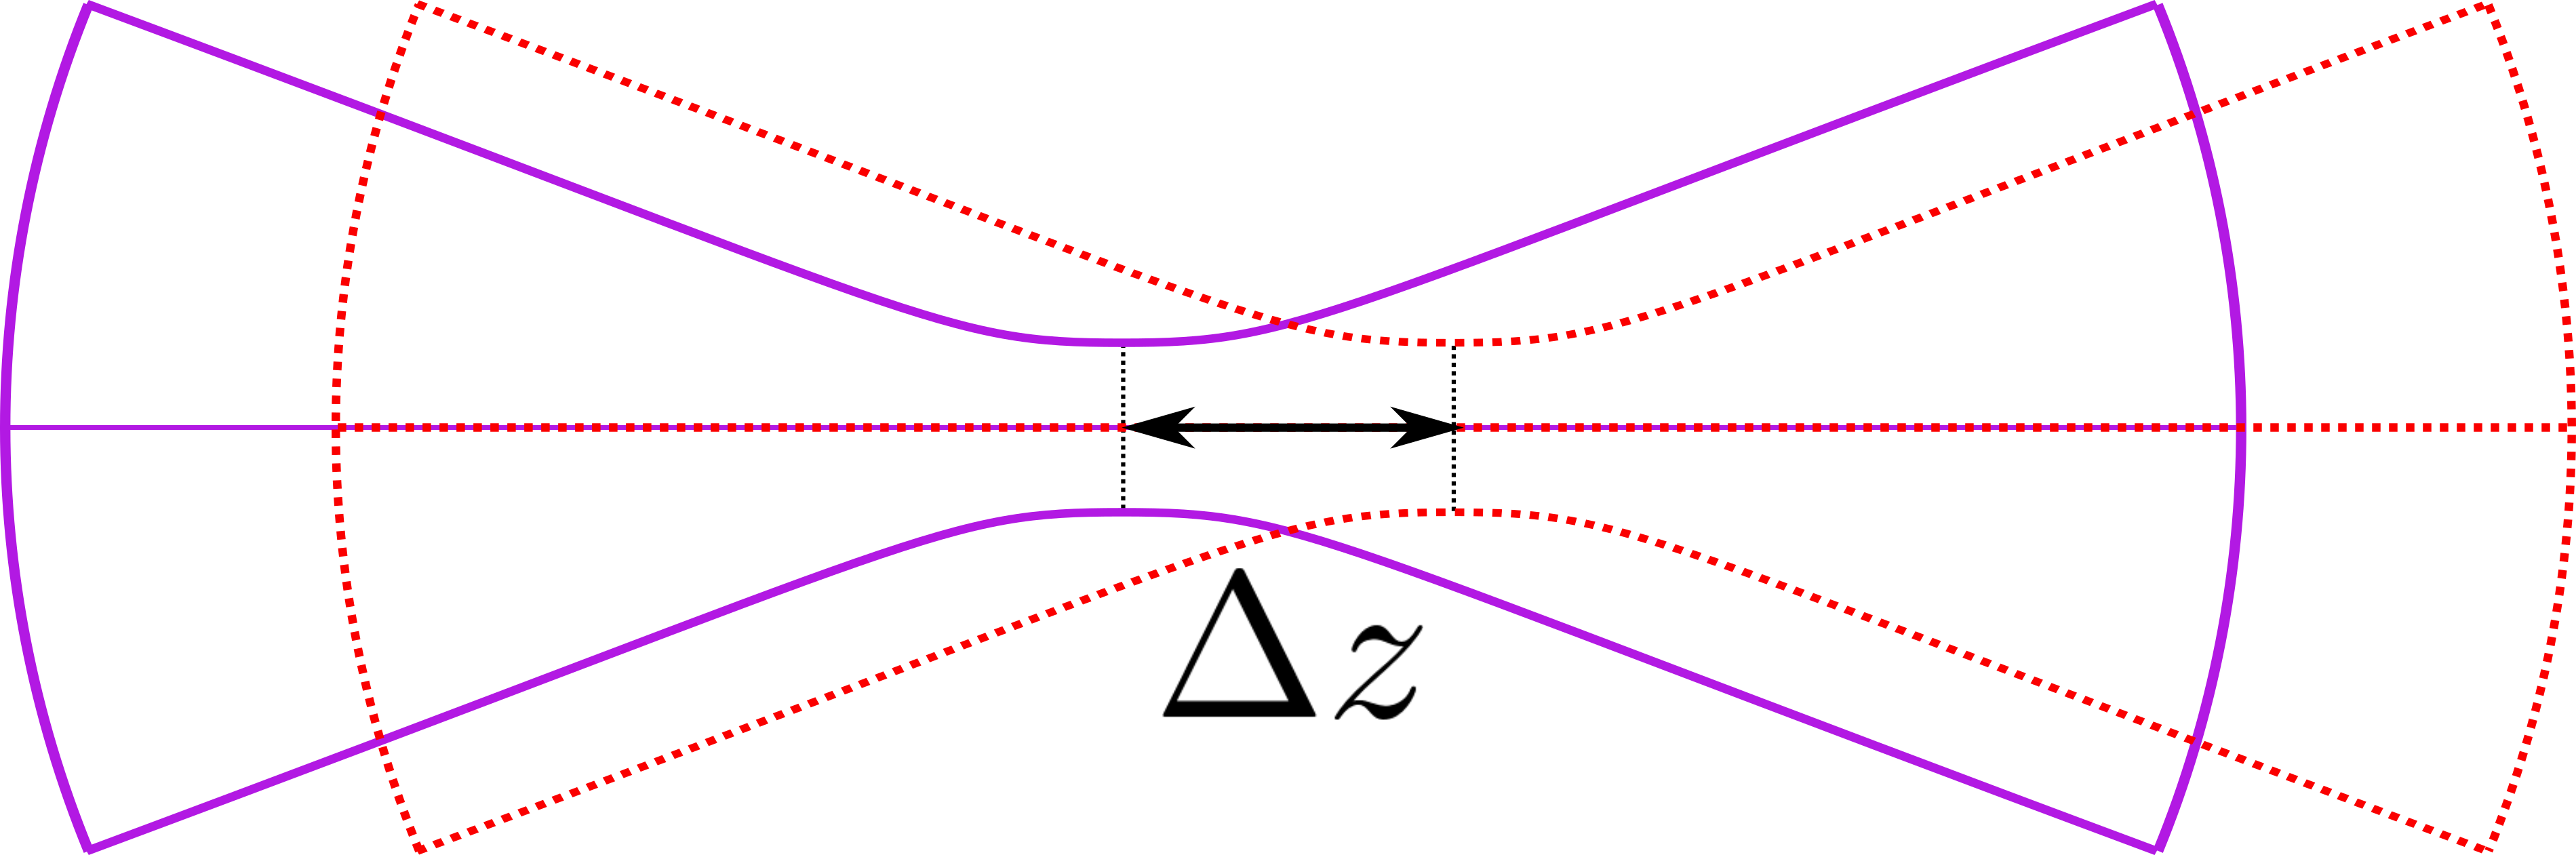
\includegraphics[width=\textwidth]{../Figures/BeamWaistDisplaced.png}
				\caption[]{\textbf{Beam waist displaced by $\Delta z$.}}    
				\label{fig:BeamWaistDisplaced}
			\end{subfigure}
			\quad
			\begin{subfigure}[b]{0.475\textwidth}   
				\centering 
				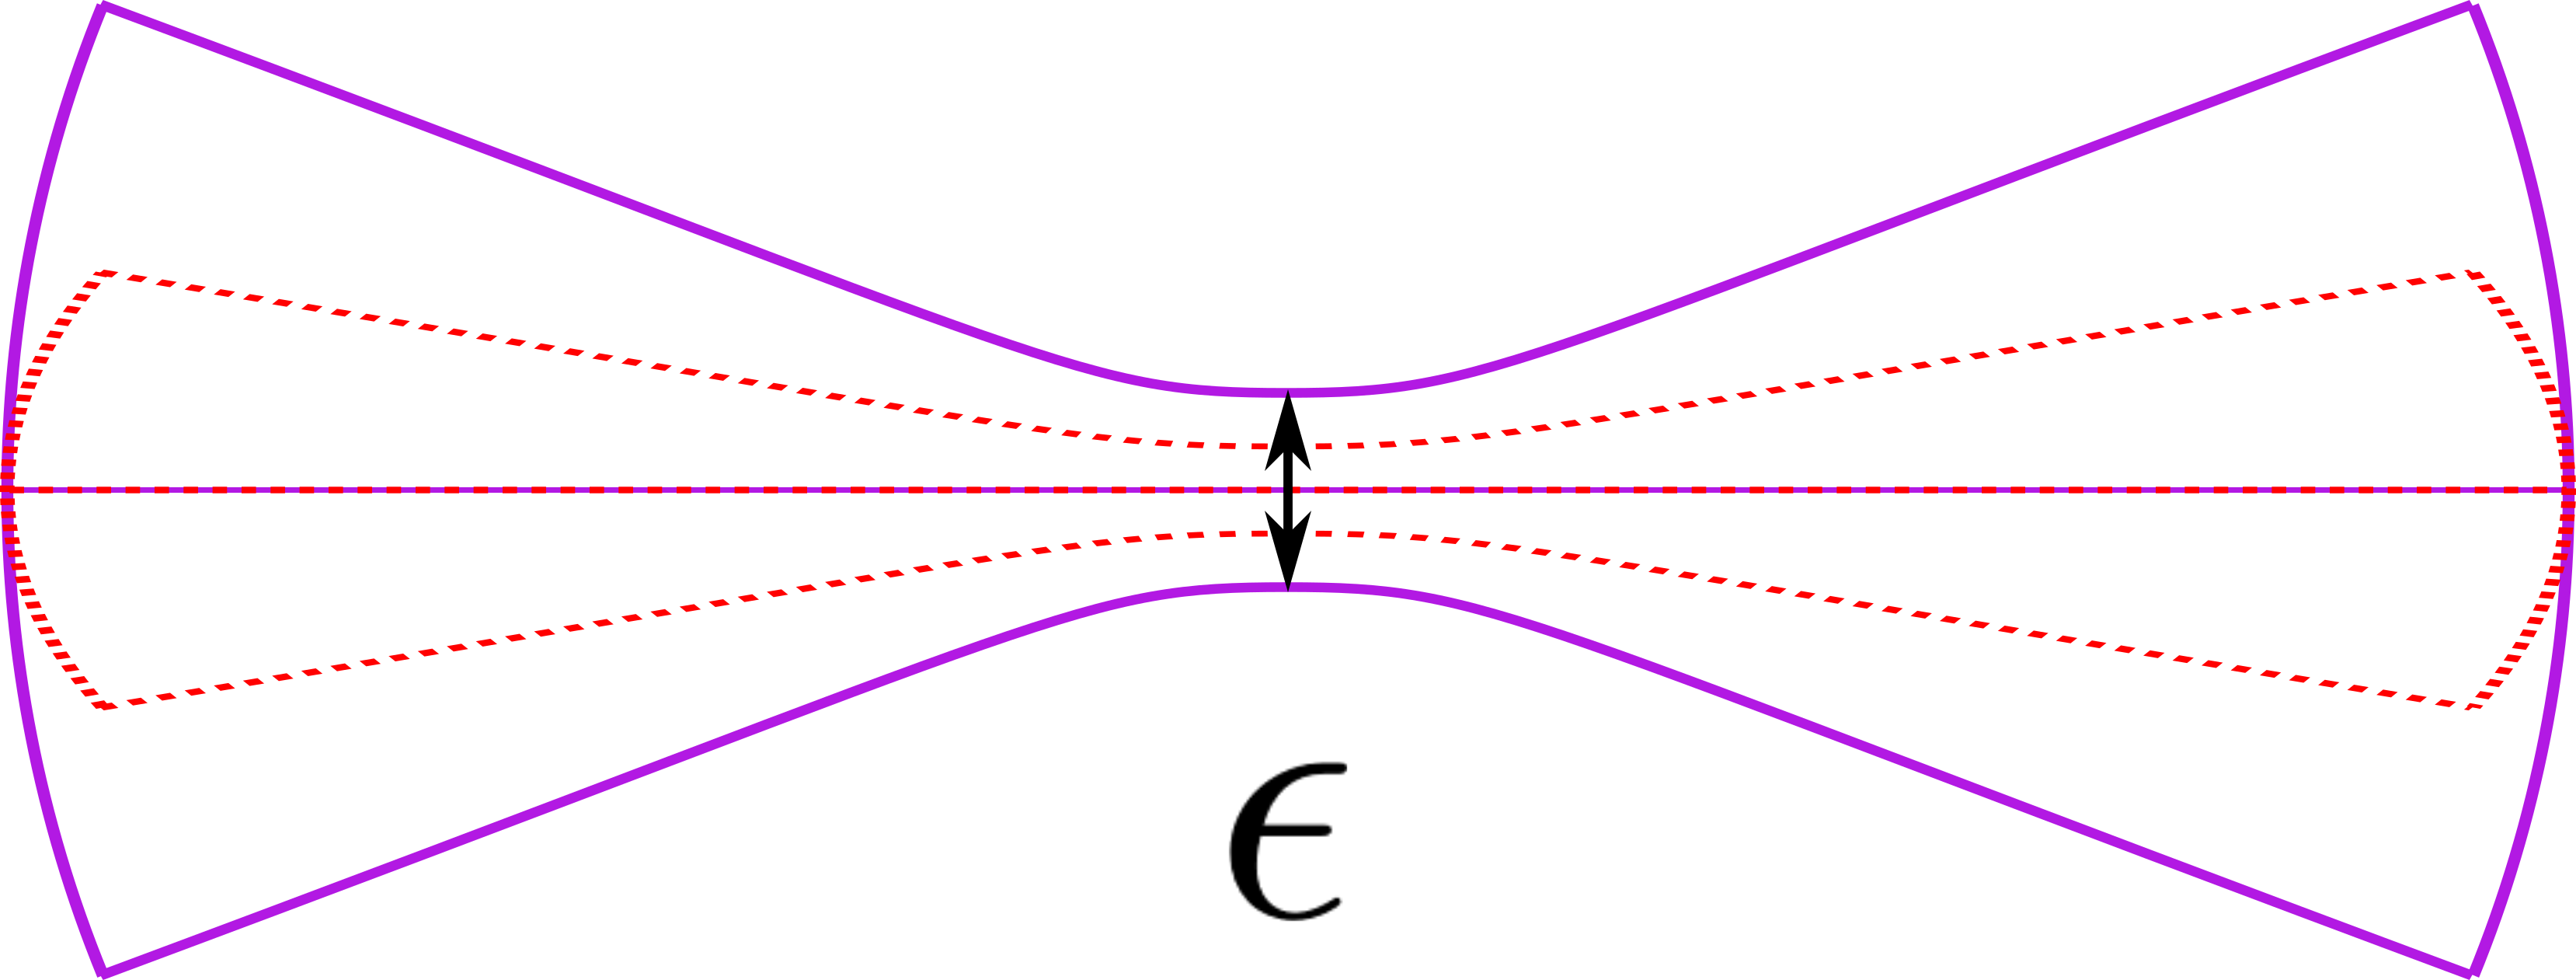
\includegraphics[width=\textwidth]{../Figures/BeamWaistEnlarged.png}
				\caption[]{\textbf{Beam waist reduced by $\epsilon$}}    
				\label{fig:BeamWaistEnlarged}
			\end{subfigure}
			\caption[Misaligment and mode mismatch between two different Gaussian beams.]  
			{\textbf{Misaligment and mode mismatch between two different Gaussian beams.}
				The purple solid curves represent the original Gaussian shape and the red dotted curves are beams which have been augmented in one degree of freedom.  It is important to note that using this representation uses the eigenmode of the cavity as a starting basis, if one were to create these misalignments using the actual optics, there needs to be a linear combination of rotations or curvature changes.
			}
		\end{figure*}
		
		\section{Wavefront Sensing}\label{WFS}
		In Chapter \ref{sec:michelson} and \ref{sec:DRMI}, a heterodyne detection scheme was used to sense the longitudinal degree of freedom for optical cavities.  Analogously, a technique using sidebands can employ a modal decomposition of the full electric field which allows the use of wavefront sensors to extract an error signal.  Hefetz et.al \cite{HefetzWFS} created a formalism to describe the use of wavefront sensors by creating frequency sidebands which accumulate a different Gouy phase than the electric field at the carrier frequency when passed through the optical system.  By observing the demodulated signal of the intensity, it is possible to obtain a linear signal that corresponds to a physical misalignment or mode mismatch.  Fundamentally, the purpose of wavefront sensing is to detect the content of higher order modes due to physical disturbances of the optical cavity and by extension, it is examining the difference between the incoming beam and the cavity eigenmodes.
		
		Consider a general equation for an electric field which is a linear combination of all higher order modes of the complex amplitude
		\begin{equation}
		E(x,y,z) = \sum\limits_{m,n}^{\infty} a_{mn} U_{mn}(x,y,z)
		\end{equation}
		where $ U_{mn}(x,y,z)$ are the eigenmodes described in equation \ref{HG} (or \ref{LG}) and $a_{mn}$ is the complex amplitude.  It is also convenient in the following analysis to use vectors when describing the composition of the electric fields.
		\begin{equation}\label{EVector}
		\ket{E(x,y,z)} = \begin{pmatrix} E_{00} 
		\\ E_{01}
		\\E_{10}
		\\E_{20}
		\\E_{02}
		\end{pmatrix}
		\end{equation}
		When creating a theory that involves laser beams, it is useful to define operators that are important in describing physical situations.  For example, laser beams propagate through space and pick up phase according to equation \ref{HG} which can be represented by the spatial propagation operator,
		\begin{equation}
		\hat{P}_{mn,kl} = \delta_{mn} \delta_{kl} \quad \text{exp}[-ik(z_2 - z_1)] 
		\\ \text{exp}[i(m+n+1)\zeta(z)]
		\end{equation}
		However, it is useful to compare how the fundamental Gaussian mode propagates compared to the higher order modes,
		\begin{equation} \label{GouyPhaseMatrix}
		\hat{\eta}_{\mu \nu} = 
		\begin{pmatrix}
		e^{i\zeta}	&0			&0			& 0 			& 0
		\\ 0		&e^{2i\zeta}	&0			& 0				& 0
		\\ 0		&0			&e^{2i\zeta}	& 0				& 0
		\\ 0		&0			&0			& e^{3i\zeta}	& 0
		\\ 0		&0			&0			& 0				& e^{3i\zeta}
		\end{pmatrix}
		\end{equation}
		From the above diagonal elements, it is clear that the higher order modes have an extra phase compared to the fundamental 00 mode, this effect will be extremely important on how an error signal can be derived from the optical system.
		\begin{equation}
		\ket{E(x,y,z_2)} = \hat{M}(x,y,z_1,z_2)	\ket{E(x,y,z_1)}
		\end{equation}
		where $\hat{M}(x,y,z_1,z_2)$ is the misalignment operator.  Since we are using the paraxial approximation, the z-components of the misalignment operator are small so we can approximate $\hat{M}{(x,y,z_1,z_2)} \approx \hat{M}(x,y)$ and the expectation value is
		\begin{equation}
		M_{mn,kl}=  \bra{U_{mn}(x,y,z_1)} M(x,y) \ket{U_{kl}(x,y,z_2)}
		\end{equation}
		where the product is an integral over the transverse space $\int \!\!\! \int_{D(x,y)} \text{d}x \text{d}y$
		\begin{equation} \label{misalign_matrix}
		\hat{\Theta}_{\mu \nu} = 
		\begin{pmatrix}
		   1			&2i\theta_x		&2i\theta_y		& 0 & 0
		\\ 2i\theta_x	&1				&0				& 0	& 0
		\\ 2i\theta_y	&0				&1				& 0	& 0
		\\ 0			&0				&0				& 1	& 0
		\\ 0			&0				&0				& 0	& 1
		\end{pmatrix}
		\end{equation}
		\begin{equation} \label{mistrans_matrix}
		\hat{\mathbb{D}}_{\mu \nu} = 
		\begin{pmatrix}
			1					&\alpha_x/\omega_{0}	&\alpha_y/\omega_{0}	& 0 & 0
		\\ \alpha_x/\omega_{0}	&1						&0						& 0 & 0
		\\ \alpha_y/\omega_{0}	&0						&1						& 0	& 0
		\\ 0					&0						&0						& 1	& 0
		\\ 0					&0						&0						& 0 & 1 
		\end{pmatrix}
		\end{equation}
		\begin{equation} \label{waistloc_matrix}
		\hat{\mathbb{Z}}_{\mu \nu} = 
		\begin{pmatrix}
		1				&0		&0		&\Delta z_x 	&\Delta z_y  
		\\ 0			&1		&0		&0 				&0
		\\ 0			&0		&1		&0 				&0
		\\ \Delta z_x	&0		&0		&1 				&0
		\\ \Delta z_y	&0		&0		&0				&1 
		\end{pmatrix}
		\end{equation}
		where $\Delta z_{(x,y)} =  \frac{i}{\sqrt{2}} \frac{\lambda b}{2\pi\omega_{0}} $
		\begin{equation} \label{waistsize_matrix}
		\hat{\mathbb{Z}}_{0, \mu \nu} = 
		\begin{pmatrix}
		1					&0		&0		&\Delta z_{0,x} 	&\Delta z_{0,y} 
		\\ 0				&1		&0		&0 					&0
		\\ 0				&0		&1		&0 					&0
		\\ \Delta z_{0,x} 	&0		&0		&1 					&0
		\\ \Delta z_{0,y} 	&0		&0		&0					&1 
		\end{pmatrix}
		\end{equation}
		where $\Delta z_{0,(x,y)} =   \frac{1}{\sqrt{2}} \frac{\omega'-\omega_{0}}{\omega_{0}} $
		
		\subsubsection{Gouy Phase}
		Understanding the relationship between Gouy phase as defined by \ref{gouy} and how the term is used colloquially within the LIGO experimental community is not very straightforward.  Gouy phase given by equation \ref{gouy} is the phase lag between a Gaussian beam and a perfect plane wave that occurs as a function of propagation along the $\hat{z}$-axis which ranges from $\zeta(z) = \pm \pi/2$ for $z =\pm \inf$.  Physically, this could be interpreted as the difference between the laser beam behaving like a plane wave when $z\approx0$ (or near field) and eventually evolving into a spherical wave when $z\approx \pm \inf$ (or far field), see Figure \ref{fig:GaussParams}.  Although this phenomenon is interesting mathematically, most texts do not consider how to practically use or measure the Gouy phase.  In LIGO technical notes and electronic logs, the Gouy phase of sensors or actuators is often used to describe where along the beam path the piece of equipment is located.  This will indicate what degree of freedom is being observed or adjusted.  For example, in ray optics \cite{Saleh} a laser beam has two degrees of freedom, the displacement and angle from the optical axis.  If an actuator such as a piezo-electric transducer with an attached reflective mirror is placed near the origin or focus of the laser beam, then the controlled degree of freedom is only the angle.  Alternatively, if the actuator is placed in the far field then the controlled degree of freedom is almost entirely displacement.  So to have full control over the alignment of a laser beam, it is required to have two actuators separated by 90 degrees in Gouy phase.  
		
		This is also true of sensors at various points along the $\hat{z}$-axis to determine the exact alignment of the optical beam. In practice, it is impossible to sense the true waist of an optical system because it could be inside a Fabry-Perot cavity.  So the clever designer must insert a pick-off beam to sample the transmission or reflection of the interested optical system and use a combination of lenses to create a telescope for the sensors and infers the degrees of freedom.  Then, by rotating to the two-dimensional space created by the sensors to represent the interested space spanned by the optical system's degrees of freedom; colloquially, this is known as a sensing matrix.  Using this method, sensors do not have to be exactly at the near or far field because it is only required that the two sensors are separated by $\pi/2$ in Gouy phase, in fact, it is usually easier to place one sensor at $+\pi/4$ and the other at $-\pi/4$. Unfortunately, there is no transducer that directly measures the Gouy phase so in order to \textit{determine} the Gouy phase of a particular sensor or actuator, one must model the beam propagation and fit the waist location.
		
		Another way which Gouy phase is presented in many LIGO discussions is regarding the round trip accumulation of phase while propagating in an optical cavity.  This plays an important role because the round trip Gouy phase is directly proportional to the transverse mode spacing.  Recall that the free spectral range of a cavity is equal to $f_{\text{FSR}} = c/2L$ which sets the frequency separation between the fundamental modes, and that the Gouy phase propagation for higher order modes is equal to $(m+n+1) \zeta(z)$ so these modes will effectively \textit{see} a different cavity than the zeroth.  Gouy phase can be calculated explicitly by using the ABCD formulation and relating the matrix elements to the round trip phase,
		\begin{equation}
		\zeta = \text{sgn} B \arccos \bigg( \frac{A+D}{2} \bigg)
		\end{equation}
		where A, B, C, and D are the matrix elements of the optical system.  The Gouy phase is related to the transverse mode spacing by
		\begin{equation}
		f_{\text{TMS}} = \frac{\zeta}{2 \pi} f_{\text{FSR}}
		\end{equation} 
		The extra Gouy phase that a higher order mode accrues as a function of $z$ shows up as in the frequency or cavity length domain as one sweeps through a full free spectral range using an offset in the length or frequency error signal.  This can be directly used to measure the higher order mode separation and becomes important if the cavity has a low finesse which means the fundamental Gaussian mode has a spread comparable in frequency to the first order mode then it is easy to hop from one to the other (see Figure \ref{fig:PRC_SRC_mode_scan}).
		\begin{figure}[ht]
			\centering
			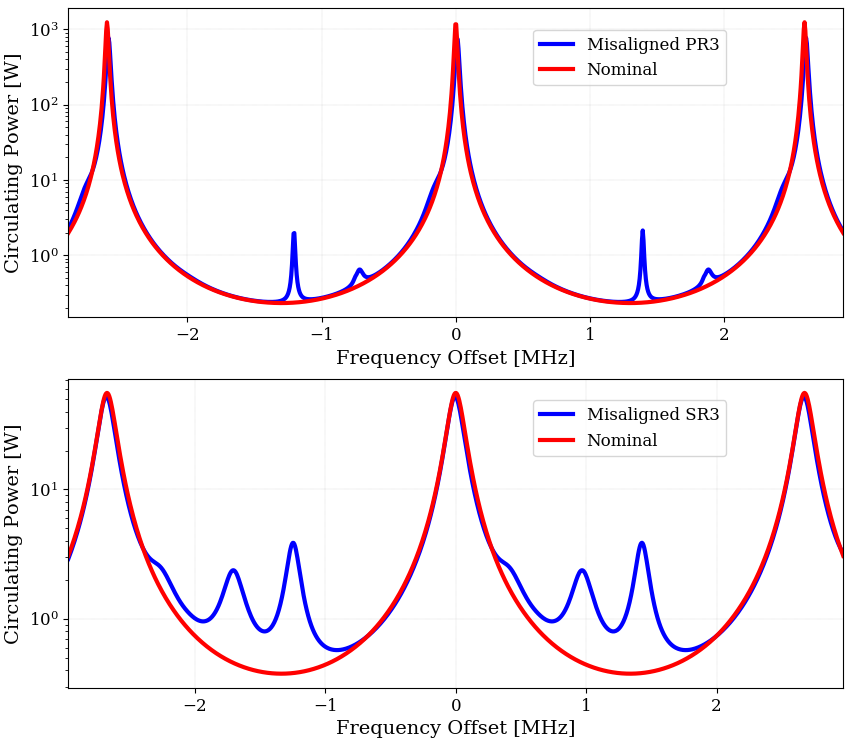
\includegraphics[width=0.55 \textwidth]{../Figures/PRC_SRC_ModeScan.png}
			\caption[A Finesse model of a longitudinal mode scan comparing the Advanced LIGO power recycling and signal recycling cavities.]
			{\textbf{A Finesse model of a longitudinal mode scan comparing the Advanced LIGO power recycling and signal recycling cavities}	The upper and lower plots represents the PRC and SRC, respectively.  The main difference between these two optical cavities is obvious when comparing the three large peaks corresponding to the 00 mode resonances.  The power recycling cavity has a much higher and sharper peak which indicates a larger finesse where as the signal recycling cavity is a much lower finesse has a broader and shorter peak.  The red traces are with nominal alignment compared with the blue lines corresponding to misalignments of PR3 and SR3 by $1 \mu$rad.  This allows higher order mode content to resonate as a function of length or frequency.}
			\label{fig:PRC_SRC_mode_scan}
		\end{figure}
\chapter{Simulating Mode-Matching with FINESSE}
In Chapter 2, the optical gain from differential arm motion was determined analytically with very few approximations but in actuality, LIGO has more degrees of freedom which make precise calculations very cumbersome.  As with most simple concepts, the complexity scales very rapidly in application to the main interferometer and mode matching is no exception so it is useful to use a full scale numerical simulation to extract as much information as possible.  FINESSE \cite{FinesseManual} \cite{FinesseTechniques} is one of the leading full-scale interferometer simulation tools which use the linear input-output relations of electromagnetic fields to model complex properties of the LIGO interferometer.  The goal of this chapter is to apply FINESSE in order to model the quantum limited noise sensitivity with mode-mismatch at various positions in the interferometer and determine which actuation points are needed for optimal matching into the output mode cleaner.  This is extremely important in the current generation of Advanced LIGO when squeezing is implemented because of the sensitivity to losses in between the optical parametric oscillator and the interferometer cavities.  By using FINESSE's ability to incorporate higher order beams and RF sidebands, it is possible to quickly and accurately model mode matching.

\begin{figure}[ht!]
	\centering
	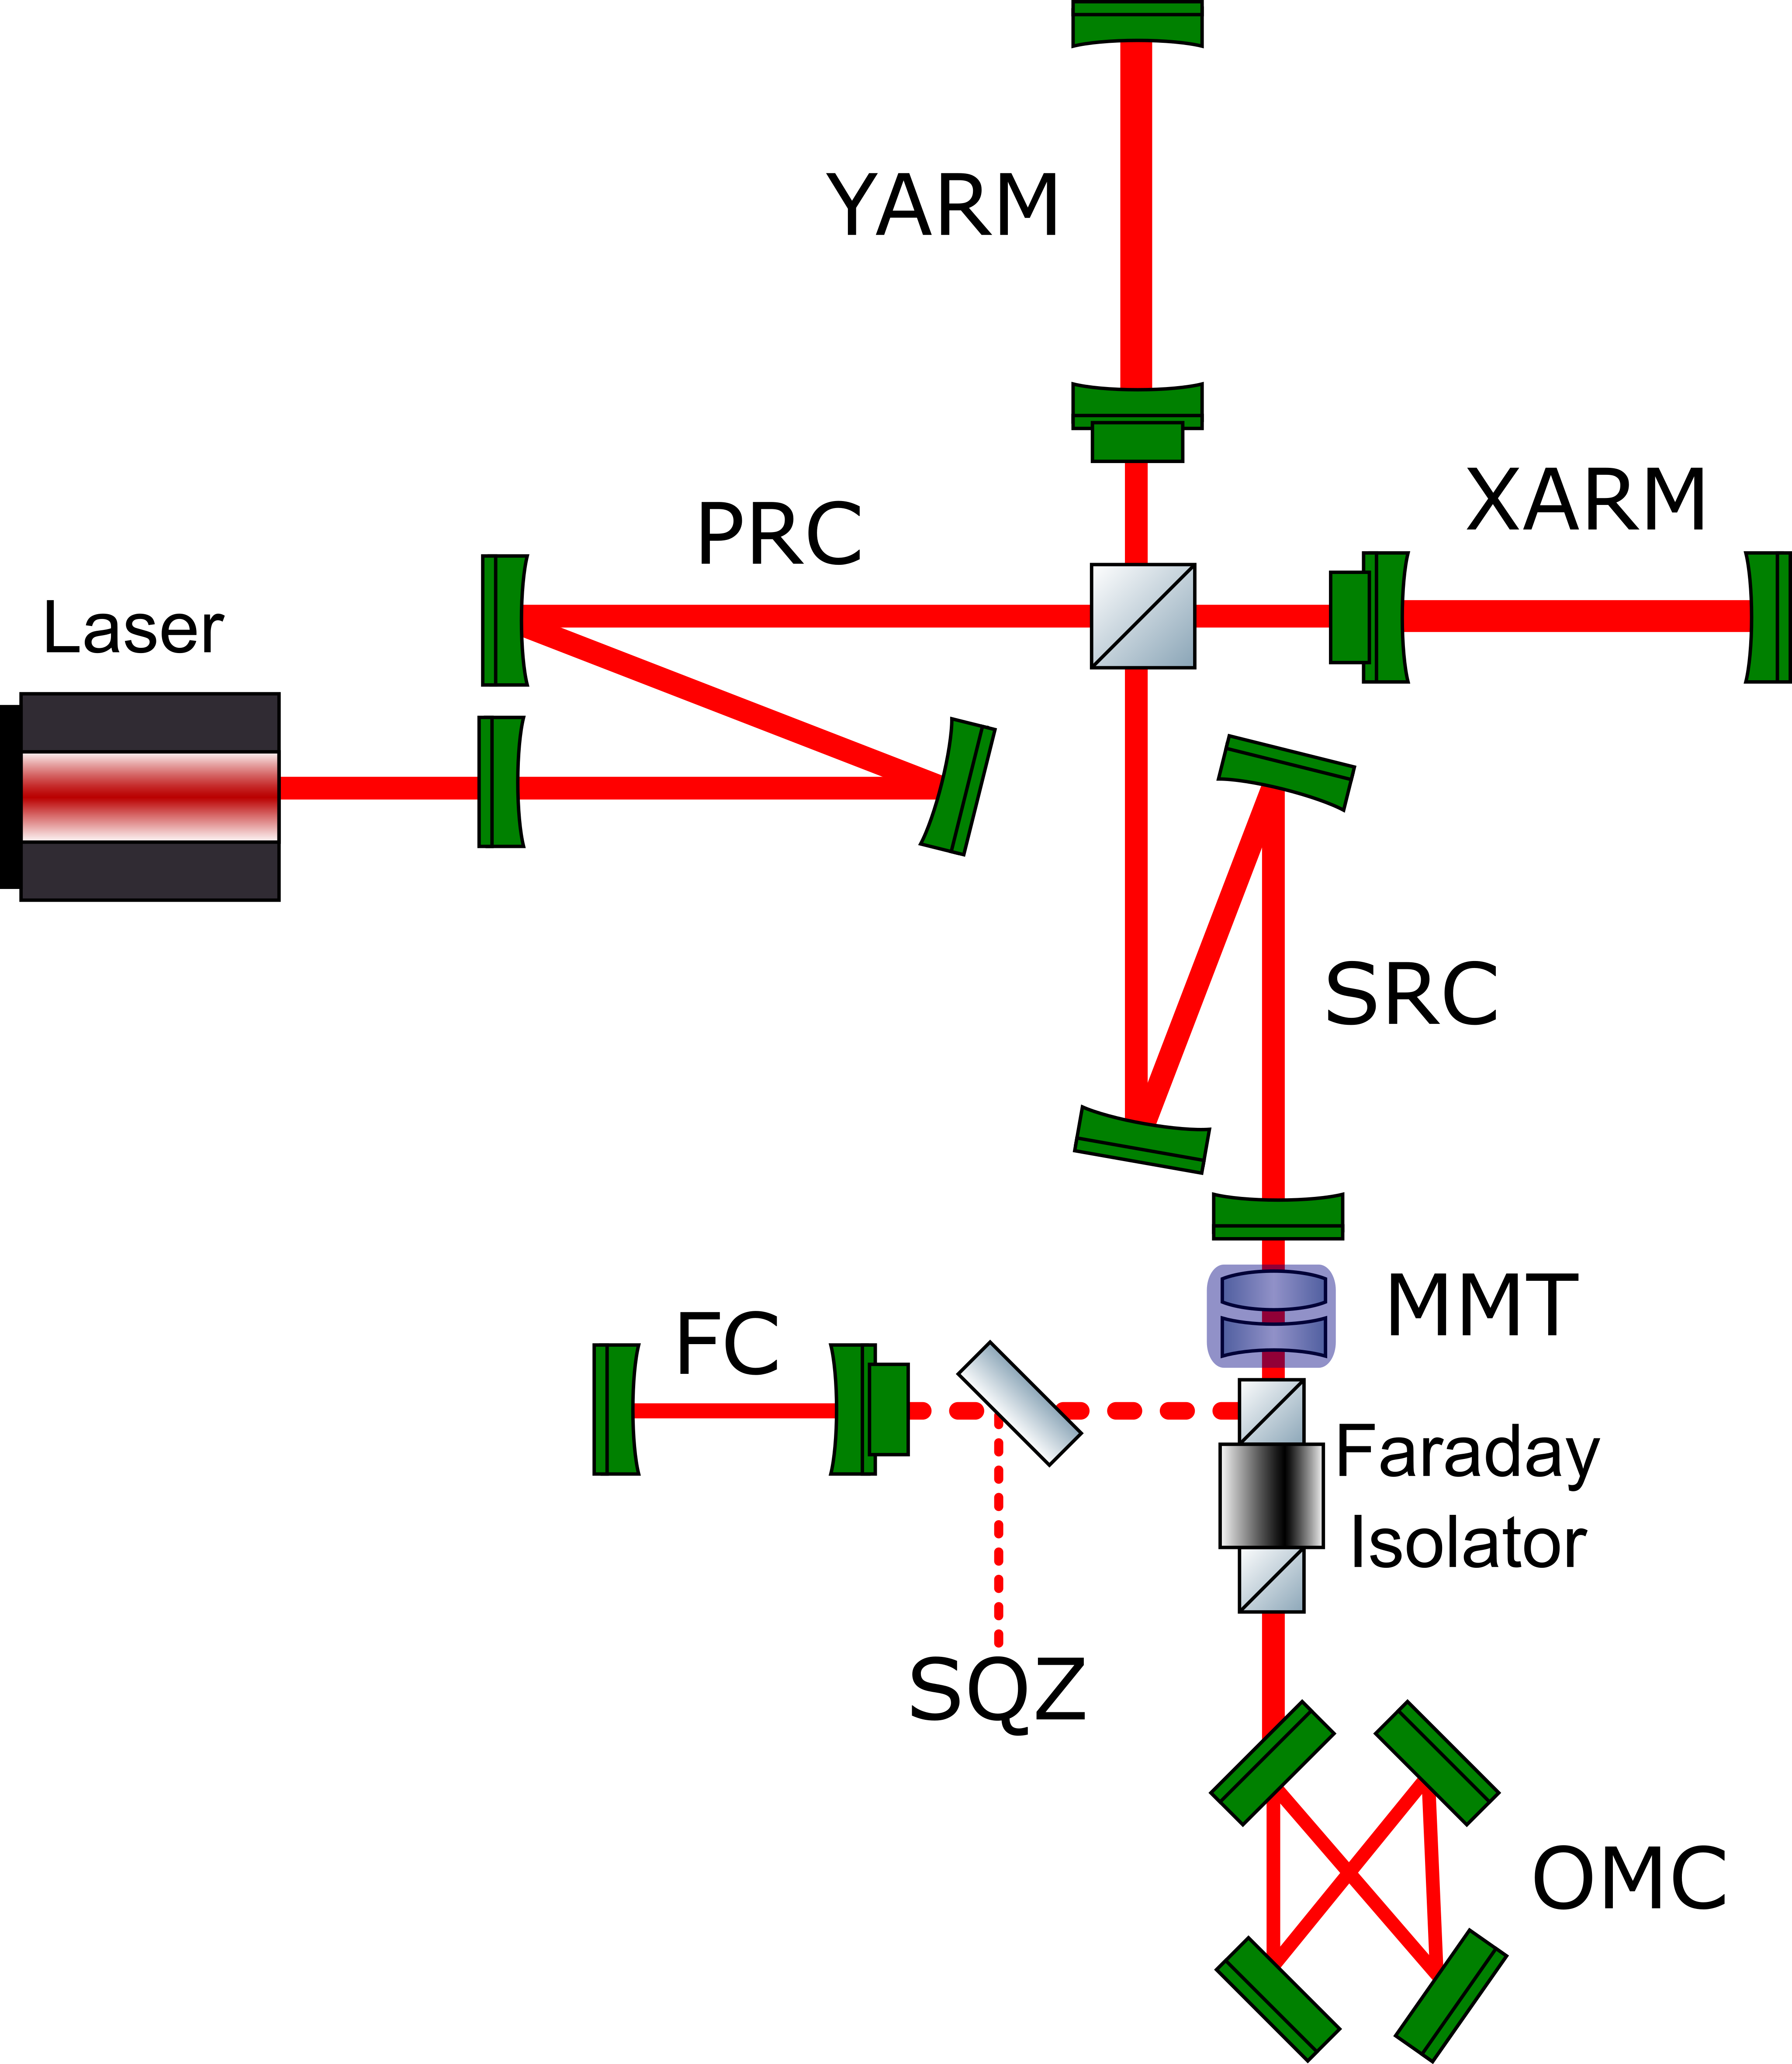
\includegraphics[width=0.8 \textwidth]{../Figures/FullIFO_FINESSE.png}
	\caption[Full interferometer simulation with FINESSE.]
	{\textbf{Full interferometer simulation with FINESSE.} 
		This includes squeezed light, a filter cavity, and an ideal mode matching telescope (highlighted in blue) at the signal recycling output port which can be turned on/off in order to understand the SRC mode mismatches without the lensing effects introduced when changing the SRM radius of curvature.  For brevity, the input mode cleaner is omitted in the schematic but is also a resonant cavity in the simulation.  Optical parameters are taken from the as-designed values for advanced LIGO and a few key variables are replaced with H1 specific constants.
	}
	\label{fig:IFO_FINESSE}
\end{figure}

	\section{FINESSE Simulations}
	The power of numerical simulations has an interesting dual advantage, firstly, optical parameters which are historically difficult to measure such as Gouy phase can be directly calculated and modeled to guide in designing systems. Secondly, in places where analytical calculations become unwieldy, numerical methods can accurately describe complex parameter spaces.
		
	\begin{figure}[h]
		\centering
		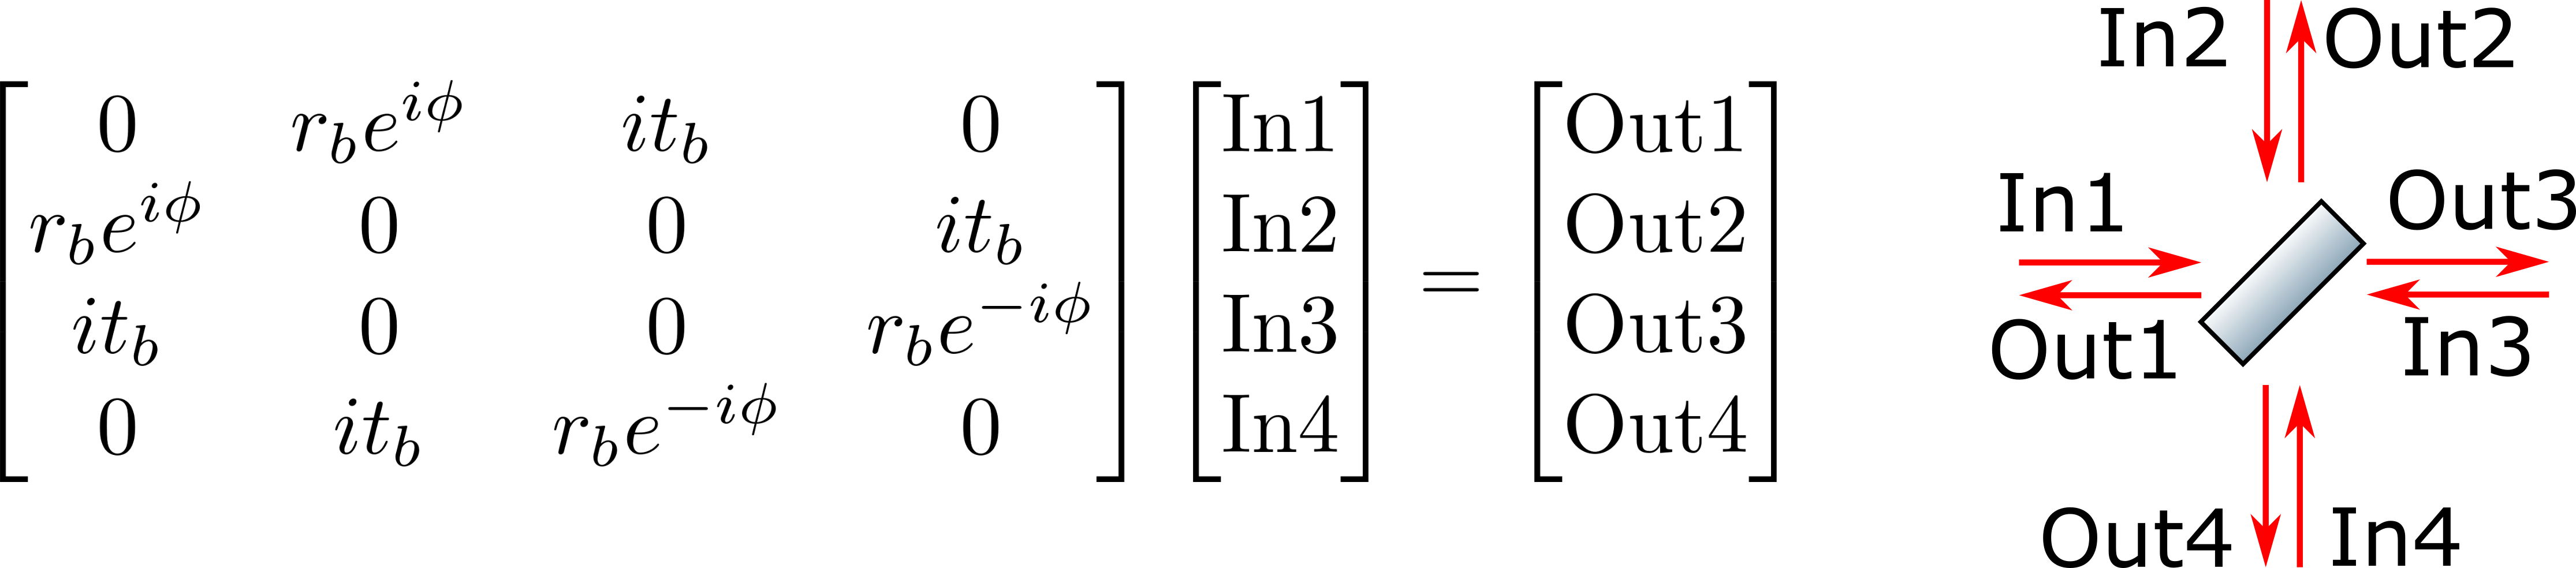
\includegraphics[width=0.8 \textwidth]{../Figures/bs_matrix_pic.png}
		\caption[How FINESSE sees a beamsplitter.]
		{\textbf{How FINESSE sees a beamsplitter.} 	An example of the coupling matrix for an arbitrary beamsplitter with reflectivity, $r_b$, and transmissivity, $t_b$. Another free parameter for a beamsplitter is the phase shift $\phi = 2 \phi_u \frac{\omega}{\omega_0} \cos(\alpha)$, where $\phi_u$ is a user defined phase that can be varied for a simulation (such as dithering), $\omega$/$\omega_0$ is the ratio of the reflected to incident angular wave frequency and $\alpha$ is the angle between the beamsplitter front surface and the incident field vector In1.  As it turns out, most of the resonators in the following simulations use beamsplitters to represent the cavity mirrors.
		}
		\label{fig:FINESSE_bs}
	\end{figure}
	An Advanced LIGO configuration file \cite{FinesseH1} which utilizes the as-designed values for the lengths and optical parameters serves as a good starting point for simulating the entire interferometer.  To incorporate more realistic numbers, in-situ measurements were taken at Hanford with a beam profile at HAM6 to understand the Gaussian beam shape entering the output mode cleaner. By defining the optical parameters and distances, FINESSE creates coupling matrices for individual components which are generally comprised of mirrors, spaces, or beamsplitters.  Some specialized components are also useful such as modulators to create sideband fields, Faraday isolators, and detectors (both amplitude and power).  For each component, there are corresponding nodes that link the entire optical system together.  The coupling matrices are compiled into an interferometer matrix and the solutions are solved numerically,
	\begin{equation}
	\hat{M}_{ij}^{\text{IFO}} \ket{x_{\text{sol}}} = \ket{x_{\text{input}}}
	\end{equation}
	where $\ket{x_{\text{sol}}}$ and $\ket{x_{\text{input}}}$ are the solution and input vectors, respectively. Generally, the right hand side is made up of laser inputs, modulator sidebands, noise, and signal sidebands. This form has incredible efficiency and can represent the entire interferometer in a single matrix with direct access to all field amplitudes.  In addition, changing optical parameters during a simulation is made easier by varying the coupling coefficients after the matrix has been calculated so the algorithm does not have to re-compute every term.
	\begin{figure}[ht]
		\centering
		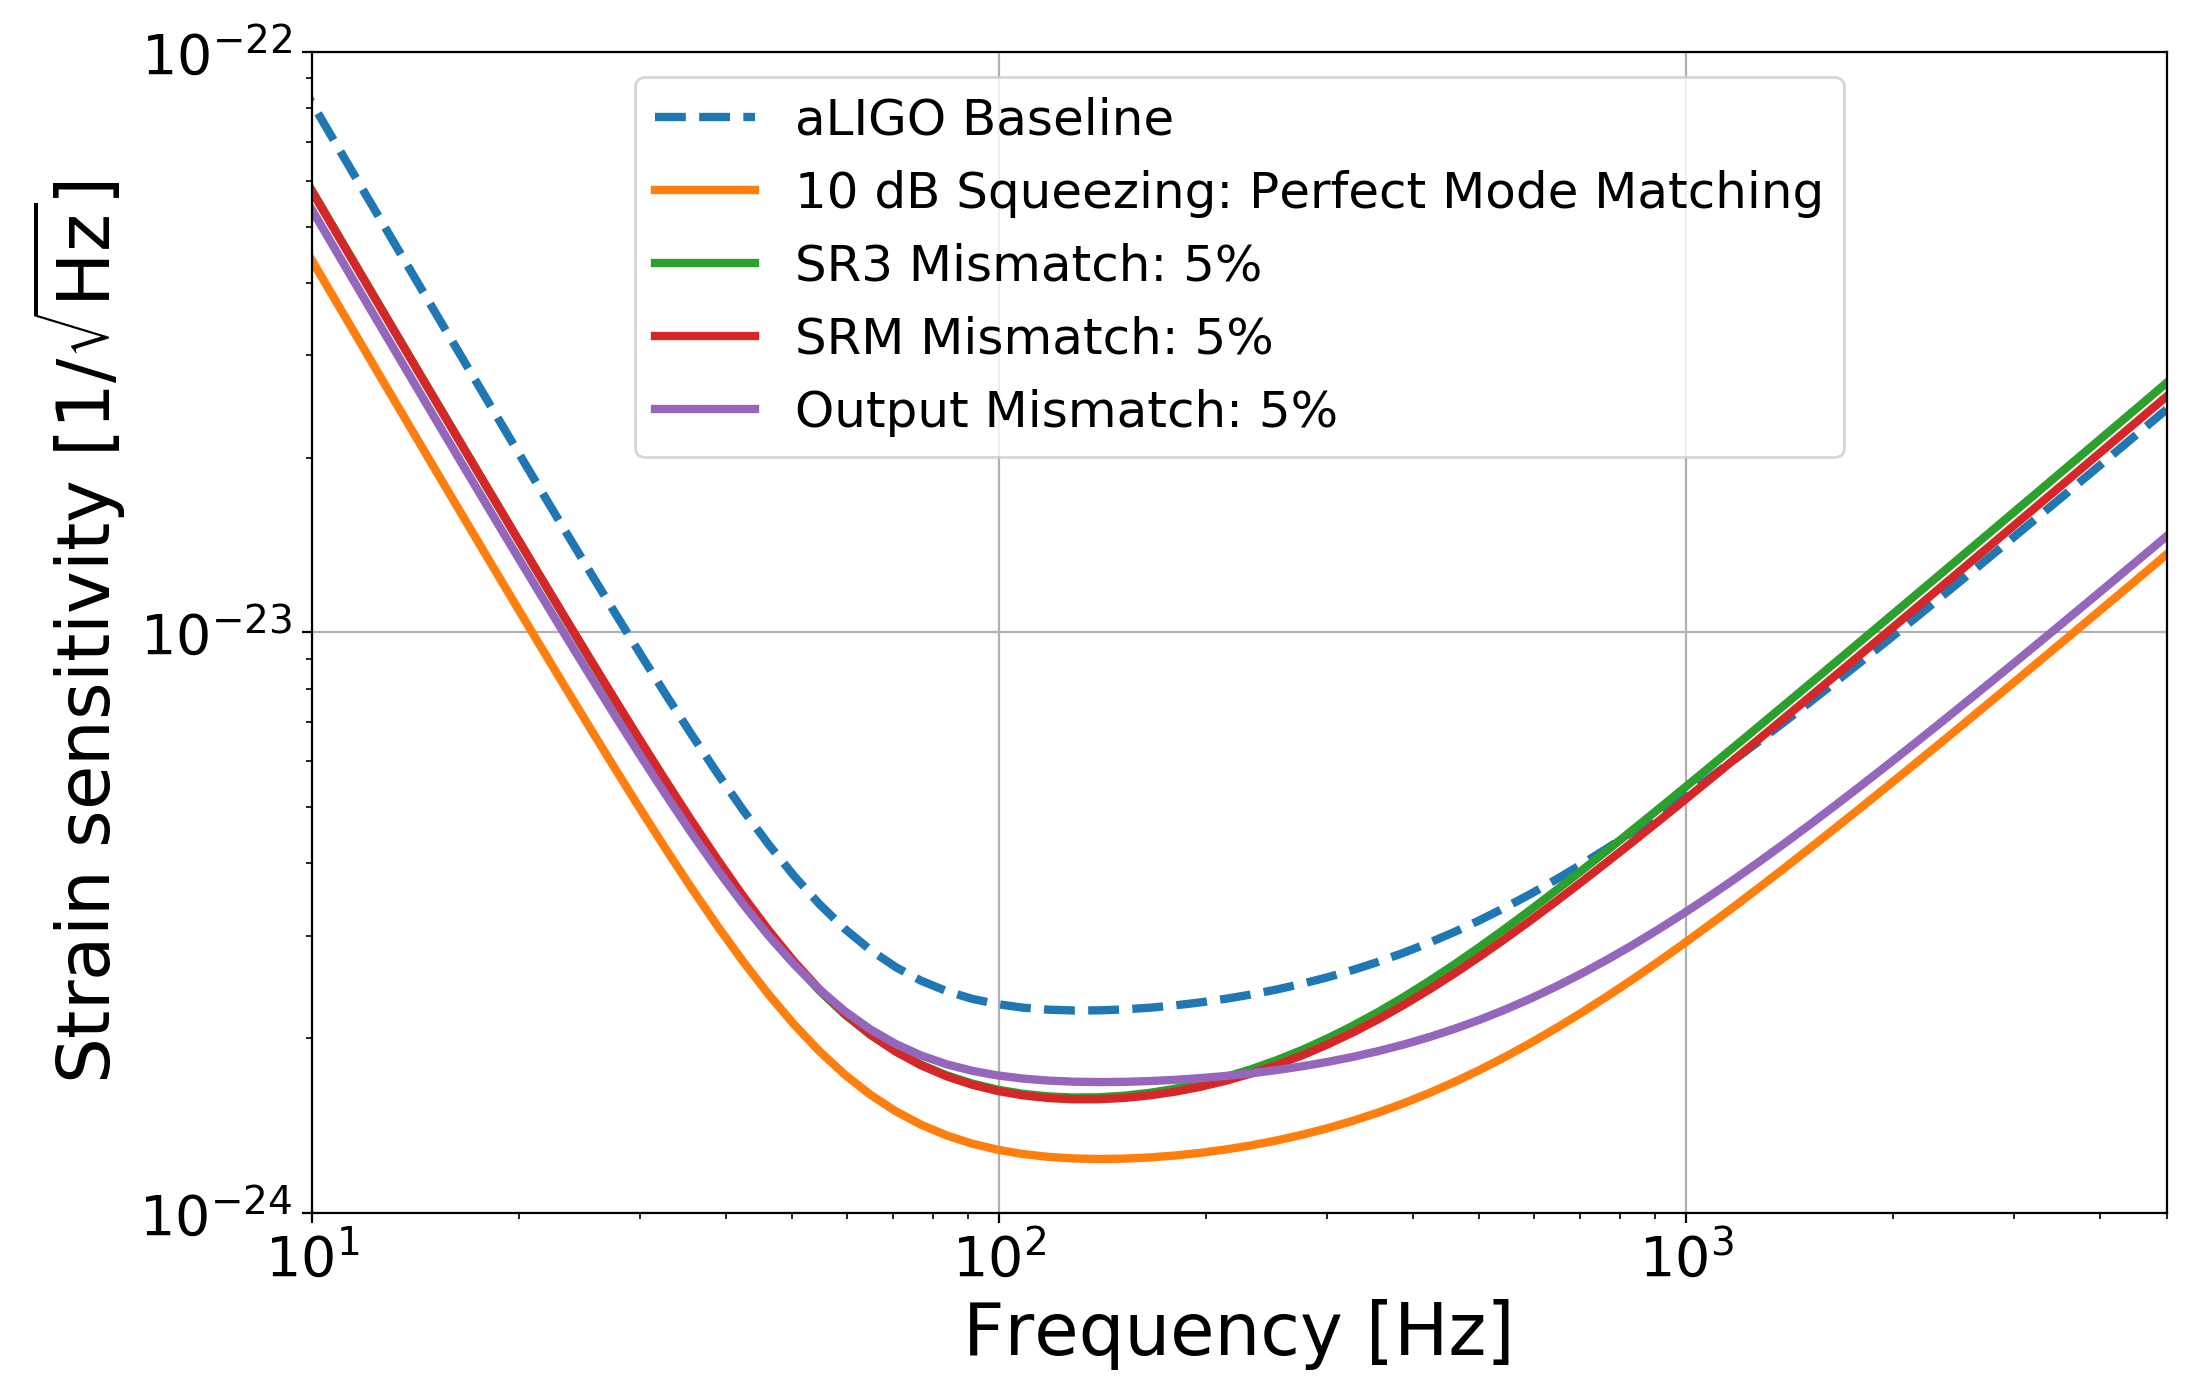
\includegraphics[width=1.0 \textwidth]{../Figures/QM_sens_compare_mismatches.png}
		\caption[Quantum limited sensitivity simulation to compare mismatches in the presence of squeezed light.]
		{\textbf{Quantum limited sensitivity simulation to compare mismatches in the presence of squeezed light.} 
			With 10 db of broadband squeezing, the simulation introduced mismatch at various actuators to change the mode shape at the output port.  Although there is still 5\% mismatch in each case, the introduction of quantum noise and the degradation of squeezing is much worse when introducing losses in the signal recycling cavity as opposed to the output train.  In addition, mismatching the signal recycling cavity will change the relative phase angle between the interferometer and squeezed light which has to be re-optimized.	
		}
		\label{fig:QM_lim_sens_mismatch}
	\end{figure}
	\section{Effects of Signal Recycling Mismatch}
	Beam tracing in FINESSE starts by determining the q-parameters for each user defined cavity. If there are multiple cavities, it will calculate in the order written and the last cavity in the parameter file sets the basis of populating the rest of the interferometer.  Table \ref{tbl:cav_params} shows the extracted cavity values for reference.  The algorithm continues by automatically propagating the laser beam through each node via ABCD transformation methods. For a perfectly mode-matched interferometer, the q's at each node are the same no matter which cavity basis is chosen but this is not true when introducing thermal lensing or errors for individual resonators.   At this point, it becomes extremely important to properly track the q-parameters because they are used to calculate the overall mismatch between cavities. To simplify the use of multiple coupled resonators, it is useful to turn all but one of the cavity commands off so that only one basis q-parameter is explicitly used and there is no ambiguity.  
	
	FINESSE has the ability to extract two parameters which calculate the sensitivity: noise and signal.  By default, vacuum fluctuations are present at each unused port and associated optical losses.  This methodology can be verified analytically using the full quantum mechanical description in Section \ref{Sec:QuantumNoise} and the semi-classical Schottky shot noise estimation.  For radiation pressure effects, the mechanical transfer function is defined by a simpled pendulum with $H(f) \propto \frac{1}{M \; f^2}$ dependence above the resonance frequency which is chosen to be approximately 0.1 Hz for these simulations.  As previously shown in Section \ref{Sec:QuantumNoise}, the radiation pressure effects are proportional to the input laser power and converts amplitude fluctuations into phase noise.  Naturally, this is a nonlinear equation when dealing with field amplitudes so FINESSE makes certain approximations which reduces the complexity,
	\begin{enumerate}
		\item Induced motion from radiation pressure is very small compared to the light wavelength so the equations of motion can be linearized.
		\item Signal sideband frequencies are very small compared to the optical sidebands created by the modulator such that the carrier creates a much larger radiation pressure effect.
		\item The amplitude of signal sidebands are much smaller compared to the carrier.
	\end{enumerate}
	In terms of gravitational wave detectors, these approximations are reasonable because the machines tend to operate with closed-loop control systems and in steady-state equilibrium.  Also, the signal sidebands never reach above 8 kilohertz for two reasons: astrophysical sources from compact binaries coalesce at around 1.5 kHz and the Nyquist frequency for the differential arm channel is sampled at 16 kHz so the Nyquist frequency is much smaller compared to the 9 MHz sideband from the electro-optical modulator.  
	
	To generate the signal, differential arm motion is created by varying the two arm cavity lengths 180 degrees out of phase and measuring the optical gain transfer function at the output mode cleaner transmission port.  The results can be compared directly to the analytical transfer function described be equation \ref{eq:DRFP_opt_gain} to verify the right DC amplitude and pole frequency.  Figure \ref{fig:IFO_FINESSE} shows the results of mode mismatch affecting the quantum limited noise sensitivity.
	
	With regards to the squeezer implementation, the model applies both squeezed light and a filter cavity before entering the interferometer to compare the effect of mode-matching losses on the quantum limited sensitivity.  In FINESSE, the squeezer node employs classical sideband implementation while in reality, modified vacuum is generated using the optical parametric oscillator (OPO) which is a bow-tie cavity with a nonlinear optic that is not yet handled by the available FINESSE components and the nonlinear crystal actually keeps the cavity from being geometrically unstable. So for now, it is enough to use quantum noise sidebands with defined phase and amplitude variances have two open parameters, the squeezing gain and phase angle. 
	
	LIGO's coupled optical cavities allow for a large parameter space when trying to match multiple resonators.   Changing the curvature of an optic in the signal recycling cavity will obviously change its overlap with the output mode cleaner but the effect will also vary the arm mode propagation to the OMC as well.  This will have a confusing result because it is impossible to discern whether the degradation in performance is due to the arm or SRC mismatch.  One of the ways to get around this is to implement a perfect mode-matching telescope between the SRC and OMC to keep the arm modes consistent with the output mode cleaner so that the only effect on the interferometer is a non-optimal signal recycling cavity.  The deterioration in sensitivity when mismatching the SRC has a two-fold effect, the introduction of vacuum fluctuations will degrade the squeezed field in a nonlinear fashion hence increasing the noise (even with perfect squeezing phase).  On top of that, extra SRC losses will affect the total optical signal gain at the antisymmetric port, which means sacrificing some losses in the SRC to mode match the squeezer field will not actually improve the sensitivity.  Comparatively, the extra losses introduced at the antisymmetric port before entering the output mode cleaner will only see increased losses that couple quantum vacuum.  The comparison is shown in Figure \ref{fig:QM_lim_sens_mismatch}.
	\begin{figure}[h]
		\centering
		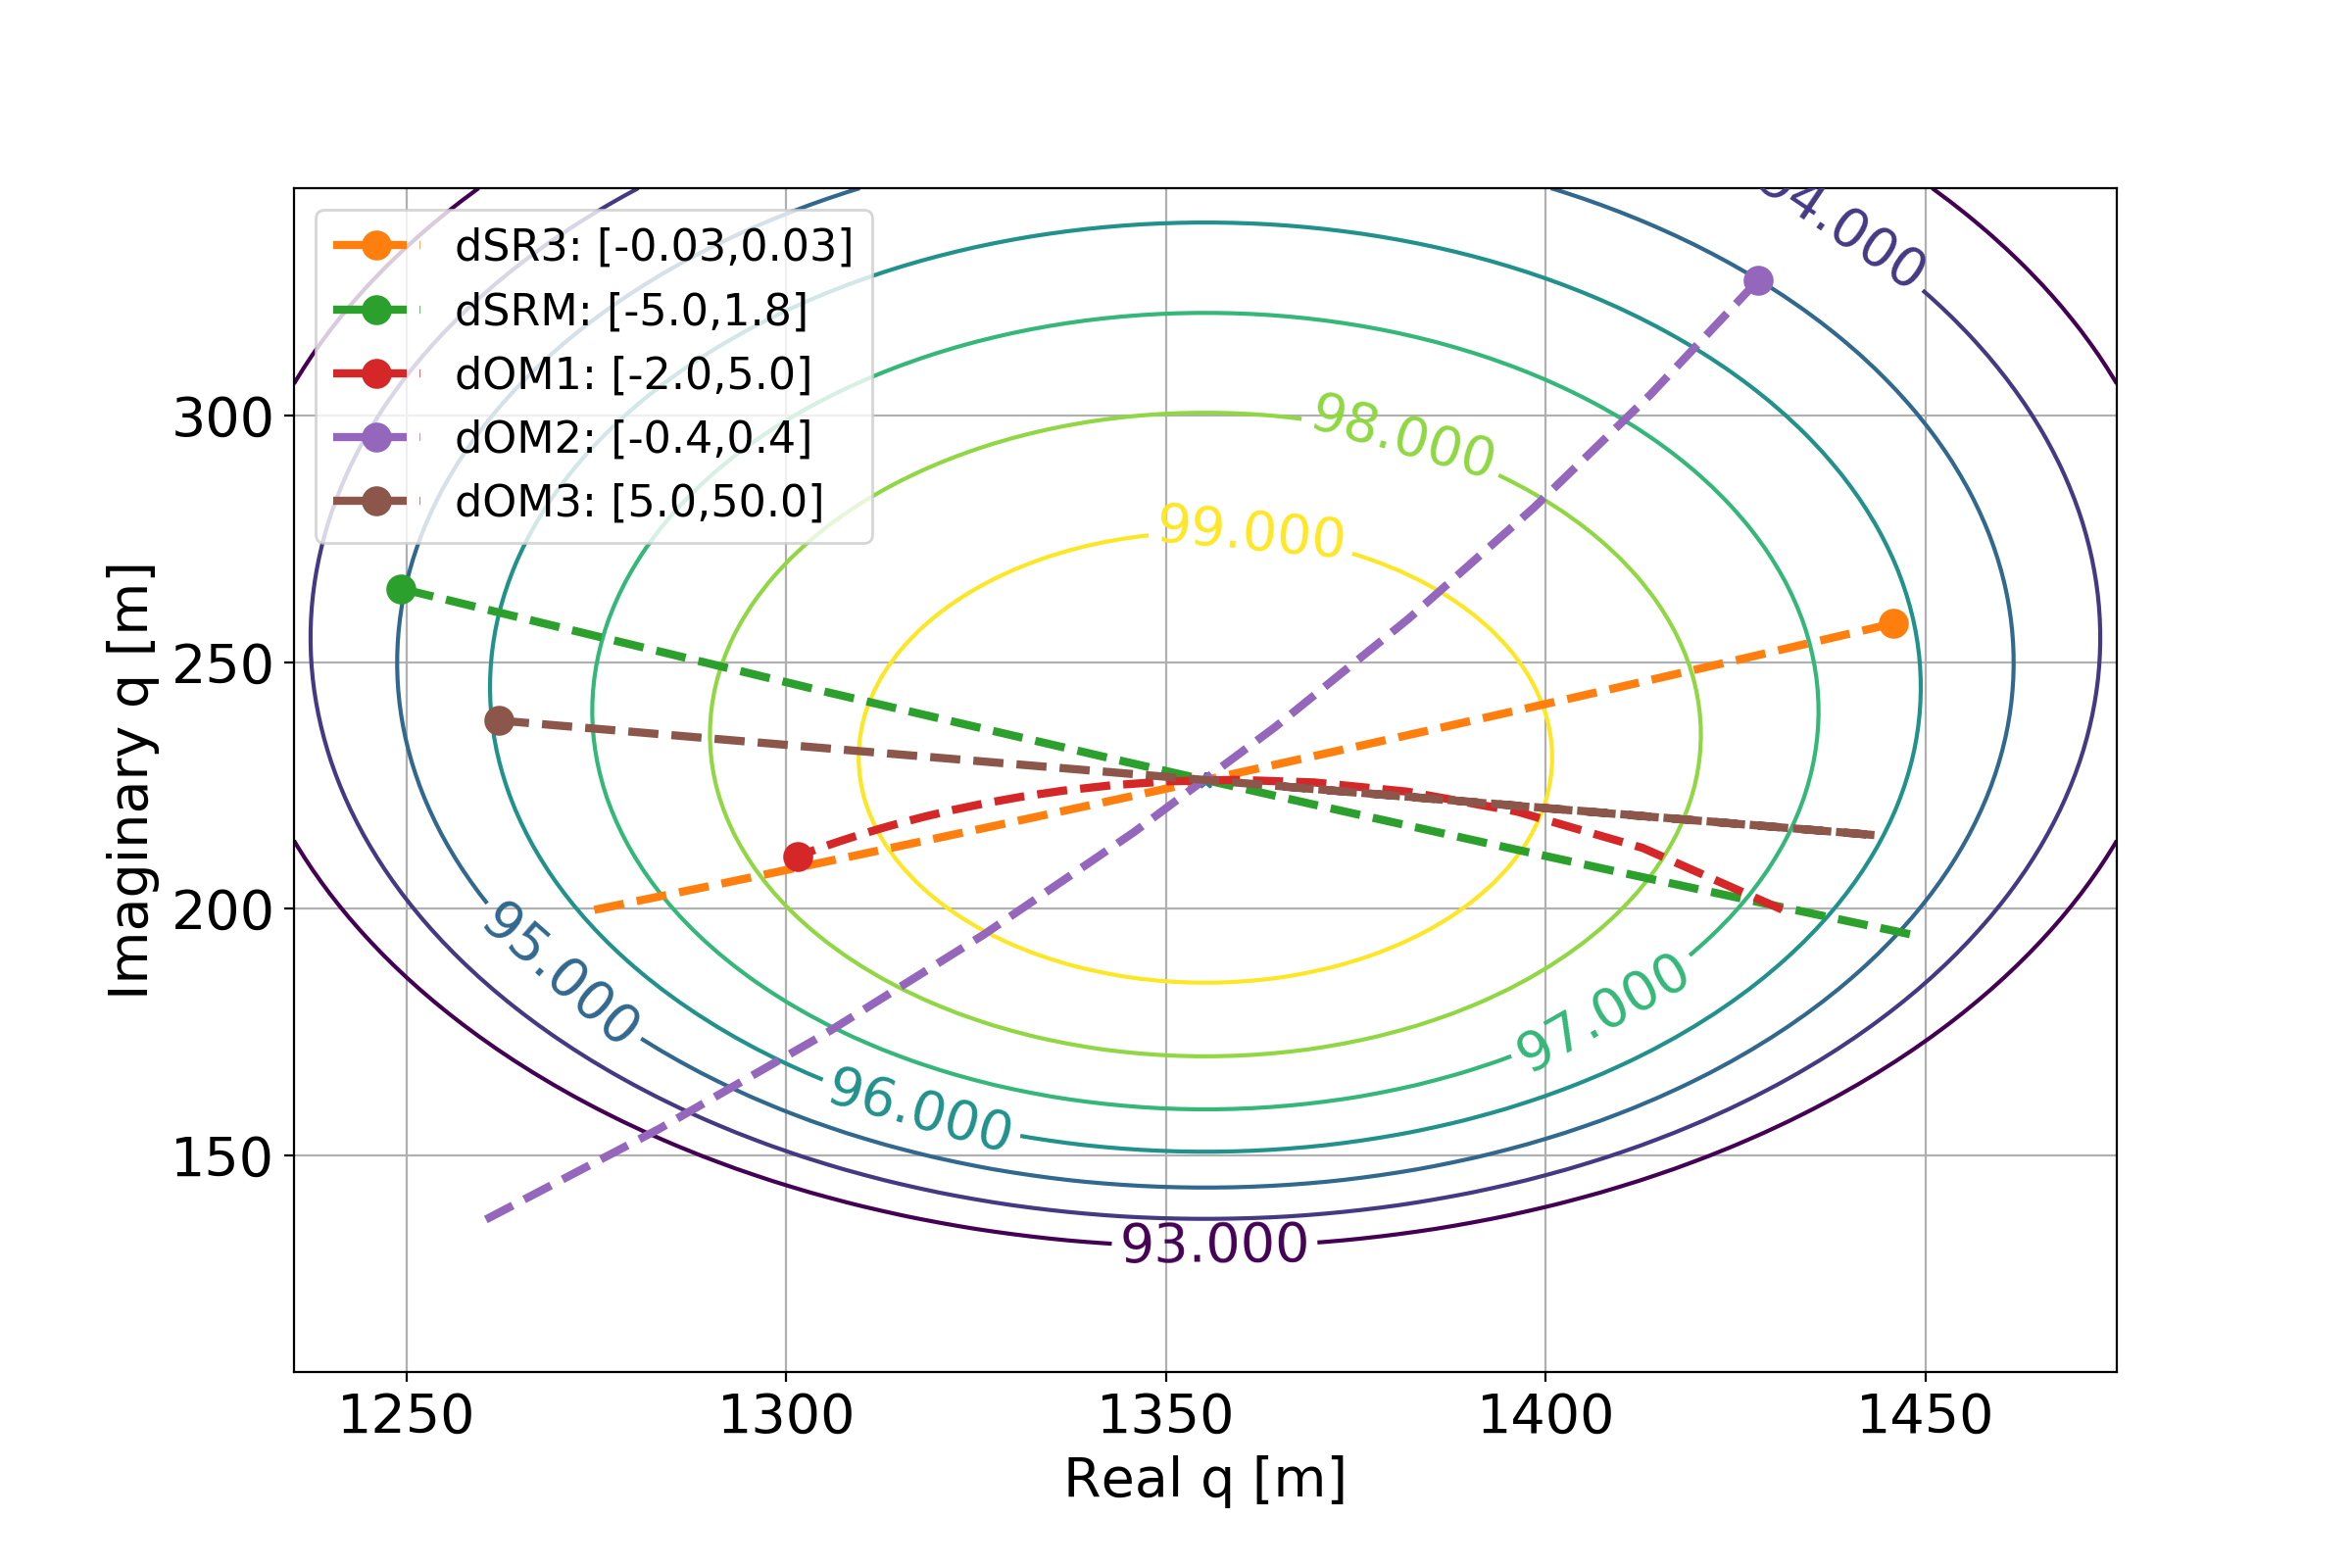
\includegraphics[width=1.0 \textwidth]{../Figures/OutputAct_Gouyphase.png}
		\caption[Simulating the output actuator phase spaces projected onto the OMC mode basis.]
		{\textbf{Simulating the output actuator phase spaces projected onto the OMC mode basis.} 
			By allowing FINESSE to do the ray tracing algorithm for the entire interferometer, it is relatively straightforward to change the radii of curvature for different optics and project the effect onto the OMC in order to understand the orthogonality when choosing mirrors for mode matching.  Interestingly, the most orthogonal actuators for small mismatches happen to be SRM and OM2, however, OM1 becomes quadratic much more quickly which leads to increased range.  The ending dots indicate the positive direction for changing radii of curvature as seen by the various optics.  Also, the change in radii of curvature in units of meters is shown on the legend.
		}
		\label{fig:act_phase_space}
	\end{figure}

	\begin{sidewaystable}
	\centering
	\begin{tabular}{|l||r|r|r|r|r|r|r|r|}
		\hline
		{} &     PRC w &    PRC S &     SRC w &    SRC S &    ARMs w &   ARMs S &   OMC w &     OMC S \\
		\hline
		\hline
		PRM   &     4.537 &    0.006 &     0.000 &    0.000 &     0.000 &    0.000 &   0.000 &     0.000 \\
		PR2   &   -45.004 &   -0.058 &     0.000 &    0.000 &     0.000 &    0.000 &   0.000 &     0.000 \\
		PR3   & -3321.891 &   -4.315 &     0.000 &    0.000 &     0.000 &    0.000 &   0.000 &     0.000 \\
		SRM   &     0.000 &    0.000 &    -5.097 &   -0.006 &     0.000 &    0.000 &   0.875 &     1.114 \\
		SR2   &     0.000 &    0.000 &  -128.889 &   -0.160 &     0.000 &    0.000 &  -2.792 &   -99.513 \\
		SR3   &     0.000 &    0.000 & -5460.964 &   -6.774 &     0.000 &    0.000 & -19.564 & -4294.447 \\
		ITMTL & -3188.263 & 4142.666 & -5254.308 & 4140.289 &     0.000 & 	 0.000 &   0.000 &     0.000 \\
		ITM   & -2310.433 & 3002.047 & -3807.633 & 3000.325 & -1827.435 & 3002.782 &   0.000 &     0.000 \\
		ETM   &     0.000 &    0.000 &     0.000 &    0.000 &  3774.807 &    4.682 &   0.000 &     0.000 \\
		OM1   &     0.000 &    0.000 &     0.000 &    0.000 &     0.000 &    0.000 &   0.164 &     0.552 \\
		OM2   &     0.000 &    0.000 &     0.000 &    0.000 &     0.000 &    0.000 &   0.511 &    -0.889 \\
		OM3   &     0.000 &    0.000 &     0.000 &    0.000 &     0.000 &    0.000 &  -0.222 &    -0.453 \\
		\hline
	\end{tabular}
	\caption[Mode matching actuation matrix for the transverse x direction.]
	{\textbf{Mode matching actuation matrix for the transverse x direction.} Each of the row elements represent actuators and columns show the affected cavity defocus $S$ or beam size $w$ per diopter change, which are scaled by the initial perfect mode matching values.  For small mismatches, the slope is assumed to be linear.}
	\label{tbl:x_act_matrix}
\end{sidewaystable}

\begin{sidewaystable}
	\centering
	\begin{tabular}{|l||r|r|r|r|r|r|r|r|}
		\hline
		{} &     PRC w &    PRC S &     SRC w &    SRC S &    ARMs w &   ARMs S &   OMC w &     OMC S \\
		\hline
		\hline
		PRM   &     5.092 &    0.006 &     0.000 &    0.000 &     0.000 &    0.000 &   0.000 &     0.000 \\
		PR2   &   -52.019 &   -0.062 &     0.000 &    0.000 &     0.000 &    0.000 &   0.000 &     0.000 \\
		PR3   & -3852.041 &   -4.569 &     0.000 &    0.000 &     0.000 &    0.000 &   0.000 &     0.000 \\
		SRM   &     0.000 &    0.000 &    -6.870 &   -0.007 &     0.000 &    0.000 &   0.870 &     1.105 \\
		SR2   &     0.000 &    0.000 &  -178.704 &   -0.169 &     0.000 &    0.000 &  -2.783 &   -99.469 \\
		SR3   &     0.000 &    0.000 & -7589.021 &   -7.189 &     0.000 &    0.000 & -19.509 & -4292.095 \\
		ITMTL & -3700.089 & 4142.316 & -7309.182 & 4139.780 &     0.000 &    0.000 &   0.000 &     0.000 \\
		ITM   & -2681.338 & 3001.794 & -5296.743 & 2999.956 & -1827.470 & 3002.700 &   0.000 &     0.000 \\
		ETM   &     0.000 &    0.000 &     0.000 &    0.000 &  3774.854 &    4.697 &   0.000 &     0.000 \\
		OM1   &     0.000 &    0.000 &     0.000 &    0.000 &     0.000 &    0.000 &   0.172 &     0.557 \\
		OM2   &     0.000 &    0.000 &     0.000 &    0.000 &     0.000 &    0.000 &   0.508 &    -0.887 \\
		OM3   &     0.000 &    0.000 &     0.000 &    0.000 &     0.000 &    0.000 &  -0.165 &    -0.344 \\
		\hline
	\end{tabular}
	\caption[Mode matching actuation matrix for the transverse y direction.]
	{\textbf{Mode matching actuation matrix for the transverse y direction.} }
	\label{tbl:y_act_matrix}
\end{sidewaystable}

\begin{sidewaystable}
	\centering
	\begin{tabular}{|l||r|r|r|r|r|r|r|r|}
		\hline
		{Parameters} &      IMC &      XARM &      YARM &        PRX &        PRY &        SRX &        SRY &        OMC \\
		\hline
		\hline
		Rayleigh Range [m]        &  13.338 &   427.807 &   427.807 &   5.314 &   5.314 &   2.132 &   2.132 &   0.708 \\
		Waist to 1st Mirror [m]   & -16.473 & -1834.220 & -1834.220 &   6.940 &   6.940 &   4.733 &   4.733 &   0.141 \\
		Cavity Length [m]      &  16.473 &  3994.500 &  3994.500 &  57.711 &  57.632 &  56.065 &  55.985 &   0.566 \\
		FSR [MHz]                 &   9.099 &     0.038 &     0.038 &   2.597 &   2.601 &   2.674 &   2.677 & 264.975 \\
		RT Gouy Phase [deg]       & 102.008 &   -48.661 &   -48.661 &  51.724 &  51.722 &  38.311 &  38.309 &  78.979 \\
		Pole Frequency [kHz]      &   8.636 &     0.045 &     0.043 & 309.692 & 309.939 & 409.982 & 410.283 & 321.971 \\
		Finesse                   & 526.837 &   413.523 &   436.867 &   4.193 &   4.196 &   3.261 &   3.263 & 411.488 \\
		A                         &   1.000 &    -2.559 &    -2.559 &  -0.406 &  -0.406 &  -0.591 &  -0.591 &  -0.004 \\
		B                         &  32.946 & -6225.726 & -6225.726 &  11.286 &  11.286 &   7.835 &   7.835 &   0.722 \\
		C                         &  -0.073 &     0.002 &     0.002 &  -0.148 &  -0.148 &  -0.291 &  -0.291 &  -1.387 \\
		D                         &  -1.416 &     3.880 &     3.880 &   1.645 &   1.645 &   2.161 &   2.161 &   0.386 \\
		\hline
	\end{tabular}
	\caption[Calculated cavity parameters for the advanced LIGO interferometer.]
	{\textbf{Calculated cavity parameters for the advanced LIGO interferometer.}
		The values were obtained using FINESSE's $cav$ commands which are an integral part of the beam tracing algorithm. Here, the power (and signal) recycling cavity is split into two linear resonators made up of the PRM and HR surface of the respective ITMs.  In an ideal world, the reflectivity of ITMX and ITMY are the same but can actually vary up to 5\% in the case of H1 \cite{galaxy}. This mostly affects the arm cavity Finesse but can have small effects on the power recycling cavity as well.}
	\label{tbl:cav_params}
\end{sidewaystable}

\chapter{Experimental Mode Matching Cavities at Syracuse}
In conjunction with Sandoval et al \cite{Fabian_Thesis}, the table-top adaptive mode matching experiment was able to show the feasibility of a fully dynamical system at Syracuse University.  Most of the work done by the author was focused on converting and upgrading the real-time digital sysem (RTCDS) from being used by the optical trap experiment \cite{OpticalTrap} to adaptive mode matching and interfacing the RF sensors into the digital system.  There is also a section on the usage of cylindrical lenses and quadrant photodiodes as a viable method of extracting a mode matching error signal.

\section{Commissioning the Real Time Digital System}
	Dynamic control systems require both actuators and sensors which are interfaced in a real-time manner and this requires the use of analog-to-digital (ADC) and digital-to-analog (DAC) converters.  A LIGO standard system uses a front end computer that reads in data and processes the signals based off a Simulink graphical model that allows for simple logic, mathematical operations, and frequency dependent filtering.  The real time data acquisition code is user-interfaced with a Motif Editor and Display Manager (MEDM) that is able to report and execute variables such as gains and matrix elements.
	
	\begin{figure}[h]
		\centering
		\frame{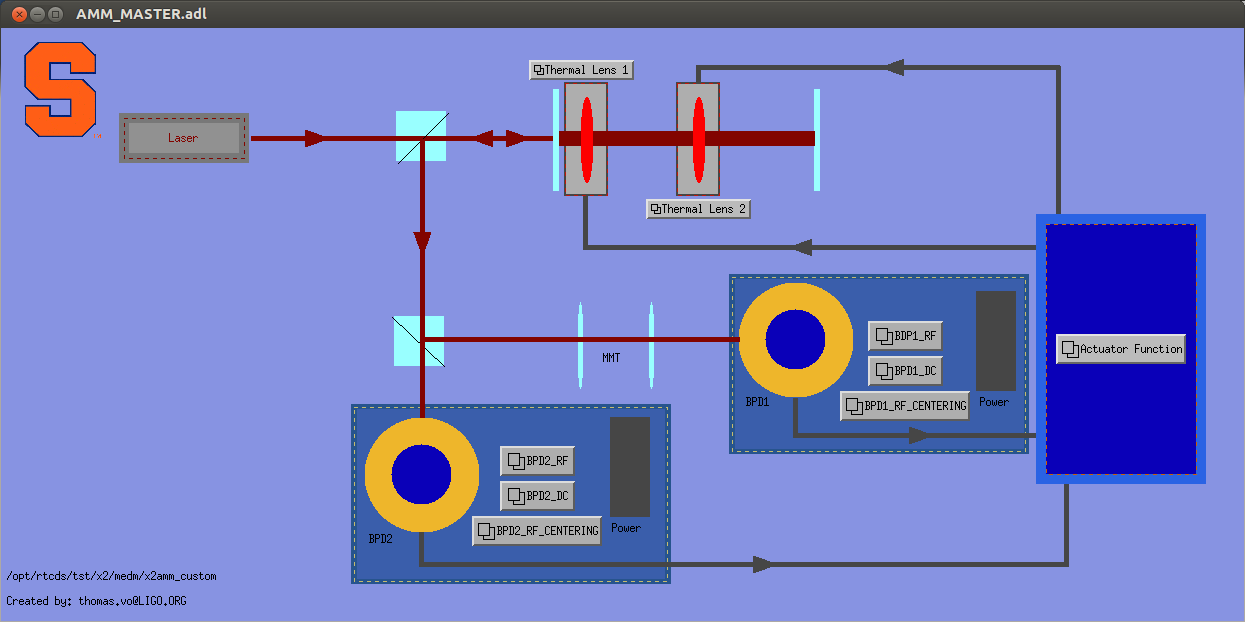
\includegraphics[width=1.0 \textwidth]{../Figures/AMM_MASTER.png}}
		\caption[MEDM master screen for adaptive mode matching at Syracuse.]
		{\textbf{MEDM master screen for adaptive mode matching at Syracuse.}  
			Here, the demodulated error signal in reflection of the Fabry-Perot cavity is divided by a beamsplitter and fed into two RF detectors, one of which is depicted to have a mode matching telescope MMT to project a different Gouy phase to sense an orthogonal degree of freedom. Then the signal is sent to an actuator function which allows for diagonalizing the signals and can be sent to a set of thermal lens at different Gouy phases for actuation.  The adaptive lenses are actually placed in the beam path before entering the cavity but for demonstrative purposes, they are portrayed at two different Gouy phases of the resonator.
		}
		\label{fig:AMM_Master}
	\end{figure}

	\section{Sensors}
	Recall in Section \ref{WFS} that the RF modal decomposition technique relies on comparing the Gouy phase of higher order modes to the fundamental Gaussian mode with an array of RF photodiodes in order to extract an error signal. The complication arises when using this method to extract the beat note between the fundamental mode and symmetric donut mode because the photodetector arrays must match the higher order mode geometry.  This is easier to deal with when trying to sense angular distortions from a misaligned cavity because the 01 and 10 modes can be sensed with a split photodetector, however, using a quadrant photodiode will not work to sense mode mismatch due to the cylindrical symmetry of the 02 and 20 modes. Currently, Advanced LIGO uses no RF sensors to detect mode matching so the next sections will provide sensing methods which can be used for dynamic closed loop feedback control.
	
	\subsection{Bullseye Photodiodes (BPD)}
	It is clear that using a quadrant photodetector to measure the symmetric $U_{20} + U_{02}$ mode which arises from mismatch is futile because the integrated power on each side will be exactly the same due to donut mode symmetry. So it is simplest to try subtracting the inner beam power from the outer ring of the electric field in order to measure a phase difference using a specialized RF photodiode called a Bullseye Photodetector shown in Figure [].  This method is proven to already work in the Enhanced LIGO era \cite{MuellerMM} and is the most natural extension of the angular wavefront sensing/controls that is implemented in Advanced LIGO.
	
	\subsubsection{BPD Calibration}
		To use the BPDs, there are a few steps required in designing the optical setup which is different than the standard PDH or WFS method.  Most notably, the beam size incident on the BPD must be tuned such that the zero crossing of the ($U_{20} + U_{02}$) matches the boundary between the inner and outer segments.  This condition is met if $\omega_{0} = \sqrt{2} r_0$ and Appendix \ref{BPDchar} shows the power ratio of the outer to inner segments when this is true,
		\begin{equation}
		\text{Power Ratio} = \frac{\text{P}_2 + \text{P}_3 + \text{P}_4}{\text{P}_1}  \\
		= \frac{e^{-2r_0^2/ \omega_{0}^2}} {1 - e^{-2r_0^2/ \omega_{0}^2 }} \approx 0.582
		\end{equation}
	
		
		Picture of BPD
		
		Pitch and Yaw sensing matrix

		Another constraint on using this method is that the Gouy phase separation between successive BPDs must be close to 45 or 135 degrees so that the error signals from each BPD can be orthogonalized, this is in contrast to angular wavefront sensors which require 90 degree Gouy phase separation.


\subsection{Mode Converters}
	The bullseye photodiodes can be difficult to calibrate and manufacture so a particularly interesting method of sensing mode mismatch is to convert the axisymmetric fields with a cylindrical telescope such that an error signal can be extracted with quadrant photodiode.  Using lenses which have two radii of curvature for each direction (x or y) with one being flat and the orthogonal is curved with some focal length, $f$.  The idea is to break the cylindrical symmetry of the donut mode (Figure \ref{fig:ModeConv}) and convert the beam into a pringle mode by advancing the phase of one axis by a factor of $\pi/2$ to create a relative sign flip.  Then, an error signal can extracted using the radio frequency quadrant photodiode that the angular wavefront sensors employ

\subsubsection{Vector formalism for laser beams and optical cavities}
	Consider an optical cavity that is longitudinally resonant on the $\text{TEM}_{00}$ mode using the Pound-Drever-Hall technique shown in Section \ref{FP} and also locked with angular wavefront sensors shown in Section \ref{WFS}. When there is a small mismatch between the waist size and position of the input beam relative to the cavity, this is equivalent to coupling the TEM-00 mode into higher order modes.  Since mode matching is only concerned with coupling to the second order modes, the  resultant field in reflection ($r_{FP}$) of a Fabry-Perot resonator will have the form
	\begin{equation}\label{MMVector}
	\ket{U_{refl}} = r_{FP} \begin{pmatrix} U_{00}
	\\ 0
	\\ 0
	\end{pmatrix}
		+
	\epsilon \begin{pmatrix} 0
	\\ U_{20}
	\\ U_{02}
	\end{pmatrix}
	\end{equation}
\begin{equation}
\epsilon = \frac{1}{\sqrt{2}} \bigg(\frac{\delta w}{w_0} + i \frac{\delta z}{z_R}\bigg)
\end{equation}
where $\delta w$ and $\delta z$ are the mismatches in waist size and position, respectively.  O'Neil et al \cite{ONeilModeTransform} wrote down a formalism that explicitly showed the effects of cylindrical telescopes on the full range of Hermite Gauss modes. An arbitrary mode conversion system, $\hat{M}$, is comprised of two cylindrical lenses and can be described by two distinct operators,
	\begin{equation}
	\hat{M} = \hat{R} \hat{C}
	\end{equation} 
where $\hat{R}$ is a rotation operator that depends on a angle $\theta$ which can rotate about the axis of propagation and $\hat{C}$ is the mode converting operator which depends on the amount of phase advance seen by higher order modes.  Physically, $\hat{R}$ can be shifted by rotating the entire cylindrical telescope about the axis of propagation whereas the phase advance can be changed by choosing various focal lengths.  Since mode matching primarily couples power into the 02 and 20 modes of the cavity, we can use a 3x3 matrix.  For rotations about the axis of propagation, the operator is
\begin{equation} \label{rotation}
\hat{R}_{ij} = 
\begin{pmatrix}
1		&0										& 0 
\\ 	0		&\cos(\Delta \theta)						&\sin(\Delta \theta)
\\ 	0		&-\sin(\Delta \theta)						&\cos(\Delta \theta)			

\end{pmatrix}
\end{equation}
For the mode converter phase advance, the operator is
\begin{equation} \label{convert}
\hat{C}_{ij} = 
\begin{pmatrix}
1			&0						& 0 
\\ 	0			&e^{-i \Omega_{20}}		& 0
\\ 	0			&0						&e^{i \Omega_{02}}			

\end{pmatrix}
\end{equation}
where $ \Omega_{mn} = (m+\frac{1}{2}) \tan^{-1}\bigg(\frac{d}{z_{R,x}}\bigg) + (n+\frac{1}{2}) \tan^{-1}\bigg(\frac{d}{z_{R,y}}\bigg) $ and $d$ is the distance from one cylindrical lens to the waist.  $\Omega_{mn}$ is the amount of phase advance that a higher order mode will experience due to the mode converter.  It is important to note, the matrices above show that the Gaussian beam is only astigmatic within the region of between the cylindrical lenses and unchanged outside of the telescope.   If the beam reflected from the cavity is well mode matched to the cylindrical telescope, then a mode converter will introduce an astigmatism and vary the separate Rayleigh ranges \cite{BEIJERSBERGEN},
\begin{equation}
\frac{z_{R,x}}{z_{R,y}} = \frac{1+d/f}{1-d/f}
\end{equation}
Of course, the tuning of $\theta$, $d$ and $f$ is left up to the optical designer's choice.  The obvious selection for $\theta$ should rotate the output beam such that the pringle mode intensities are centered on the individual quadrant photodiodes.  The choice of separation distance $d$ and focal length $f$ are a bit more subtle.  

The second order coupling to higher order HG modes from mode mismatch creates a cylindrically symmetric intensity profile.  This can be broken by creating a phase difference between HG20 and HG02 such that there is a relative sign flip.  In Figure \ref{fig:Oneil_modeconv} of O'Neil \cite{ONeilModeTransform}, the only conversion that transforms the diagonal HG mode into a symmetric donut mode is with $\Delta \Omega = \pi/2$. This implies the converse is also true if one desires to transform the donut mode into an HG mode of the same order. Making this choice of phase propagation automatically constrains the optical setup and the second order mode along the lens axis will see a phase advance equal to
	\begin{equation}
	\frac{\pi}{2} = 2\bigg[\tan^{-1}\bigg(\frac{d}{z_{R,x}}\bigg) - \tan^{-1} \bigg(\frac{d}{z_{R,y}} \bigg)  \bigg]
	\end{equation} 
	\begin{equation}
	  \Rightarrow \sqrt{2} - 1 = \frac{d}{z_{R,y}} = \frac{z_{R,x}}{d}
	\end{equation}
The equation above only shows a relation between the Rayleigh ranges and the lens separation. However, by imposing mode matching conditions it is possible also constrain the focal length of the cylindrical lenses as well.
	\begin{equation}
	f = \bigg[\frac{1}{R_x(d)} - \frac{1}{R_y(d)}\bigg]^{-1} = \frac{d}{\sqrt{2}}
	\end{equation}
	where $R_i(d) = d [ 1 + (\frac{z_{R,i}}{d})^2]$.

\subsubsection{Extracting information from mode}
Mueller et al \cite{MuellerMM} showed that the error signal from mode mismatch could be extracted by using an RF detection scheme. Using this formalism, the error signal on a quadrant photodetector from a mismatched cavity after a mode converter is 
	\begin{equation}
	\begin{aligned}
	S 	\propto  \text{Im} \bigg\{ \epsilon^{*} \bigg[&\int_{A1,A3} \hat{M}^{\dagger}_{00} \bra{U_{00}} \big[\hat{M}^{\dagger}_{U_{20}} \ket{U_{20}} + \hat{M}^{\dagger}_{U_{02}} \ket{U_{02}}\big]  \, -\\
	 \, &\int_{A2,A4} \hat{M}^{\dagger}_{00} \bra{U_{00}} (\hat{M}^{\dagger}_{20} \ket{U_{20}} + \hat{M}^{\dagger}_{02} \ket{U_{02}}) \bigg] \bigg\}\\
	\propto \text{Im} \bigg\{ \epsilon^{*} \bigg[&\int_{A1,A3} \bra{U_{00}} \big(\ket{U_{20}} - \ket{U_{02}}\big)  \,-\, \int_{A2,A4}  \bra{U_{00}} ( \ket{U_{20}} - \ket{U_{02}}) \bigg] \bigg\}
	\end{aligned}
	\end{equation}
where the surface integrals are over each segment.  In the above equation, $\hat{C}_{ij} $ was chosen with $\Delta \Omega = \pi/2$ and $\hat{R}_{ij}$ should rotate the beams such that the intensities in Figure {ModeConverter} are aligned with the quadrant photodiodes.
		
\subsection{DC Mode Matching}
	The benefit to using the RF sensing scheme for generating an error signal is the automatic reduction of the higher order mode content which can use actuators to adjust the incoming mode of the beam to whatever the cavity requires.
	This is particularly useful in areas where the laser power density is high and absorption on the high reflectivity surfaces cause thermal distortions in the cavity mode.
	However, the output mode cleaner remains generally fixed in its eigenbasis such that the nominal input mode is static; in fact, the current alignment scheme uses DC quadrant photodiodes to feed back to the OMC suspensions and the control loop offsets are tuned to minimize the 10/01 modes.
	If there was a low-noise way to continually measure the beam size at two different Gouy phases prior to entering the output mode cleaner, then there could be an error signal which would be used for thermal actuators directly after the signal recycling cavity.
	This can be achieved with bullseye sensors that read power ratio relatively quickly.
	Another interesting way of measuring the mode is using a slowly rotating razer blade with known angular frequency in front of a single photodiode and inferring the error function which will directly give the beam size.
	
\chapter{Wavefront Control at LIGO Hanford}\label{chapter:MM_LHO}
	Simulations and calculations are wonderful guides to understanding and building intuition about mode matching,  no model is perfect and experiments have a way of presenting the most interesting and challenging problems.  Preparation for the third observing run (O3) required extensive work to understand Advanced LIGO's path to achieve higher arm power.  One of the most important tasks was tuning the thermal compensation and interferometer sensing/controls systems in order to maintain the power build-ups in the PRC and the long interferometer arms during nominal low noise operation.  This chapter will explain how lensing affects the interferometer fields and describe a few strategies to tune the Thermal Compensation System (TCS) at LIGO Hanford. Then, it summarizes in-situ measurements that were taken to understand the mode matching between the squeezer optical parametric oscillator (OPO) and the output mode cleaner in single bounce configuration.
	
	For Advanced LIGO, test mass heating comes from main two sources: absorption by arm cavity optics from the main interferometer beam and heat applied by the TCS which is meant to combat the wavefront distortion by applying heat in key places.  Thermal compensation currently utilizes ring heaters at all four main test masses, a disk heater at the SR3, and CO$_2$ lasers at the input test masses.
	
	\section{Hot vs. Cold Interferometers}\label{sec:hotcoldifo}
	When fully operational, the arm cavities can have approximately 150 kilowatts of circulating power. An estimated but useful description of the total arm power in each arm is
	\begin{equation}
		P_{\text{ARM}} \approx \frac{1}{2} (g_{\text{PRC}} * g_{\text{ARM}} * P_{\text{in}})
	\end{equation}
	where $g_{\text{PRC}} \approx 45$ is the power recycling cavity gain and $g_{\text{ARM}} \approx 225$ is the single arm cavity gain. For O3, the intended input power $P_{\text{in}}$ will reach approximately 30 W which means $P_{\text{ARM}} \approx 150,000$ W. A fraction of that power between (0.2-0.8 ppm), will be absorbed by the high reflectivity surface creating a \textit{thermo-elastic} effect which changes the radius of curvature. By changing the test mass curvatures, the resonant Gaussian mode will also change its profile. Additionally, the \textit{thermo-refractive} effect will vary the index of refraction within the bulk as a function of absorbed light power creating a thermal lens that turns out to be an order of magnitude larger than the wavefront distortion from thermo-elastic effects in fused silica \cite{winkler_thermaldist}.
	
	\subsection{Thermal Lensing}\label{Sec:TL_lensing}
	As seen in Section \ref{sec:DRMI}, the sideband and carrier frequencies propagate differently in the interferometer by design, which means their fields see different thermal lensing effects.  The ITM substrate which sees the thermo-refractive change from absorption will play the largest role because the carrier is not affected to first order (shown below). To understand how the fields change, the easiest way is to invoke the ABCD transfer matrix approach to track how the phase changes as they propagate through the optical system \cite{Lawrence_TCS}.
	
	\begin{figure}[ht!]
		\centering
		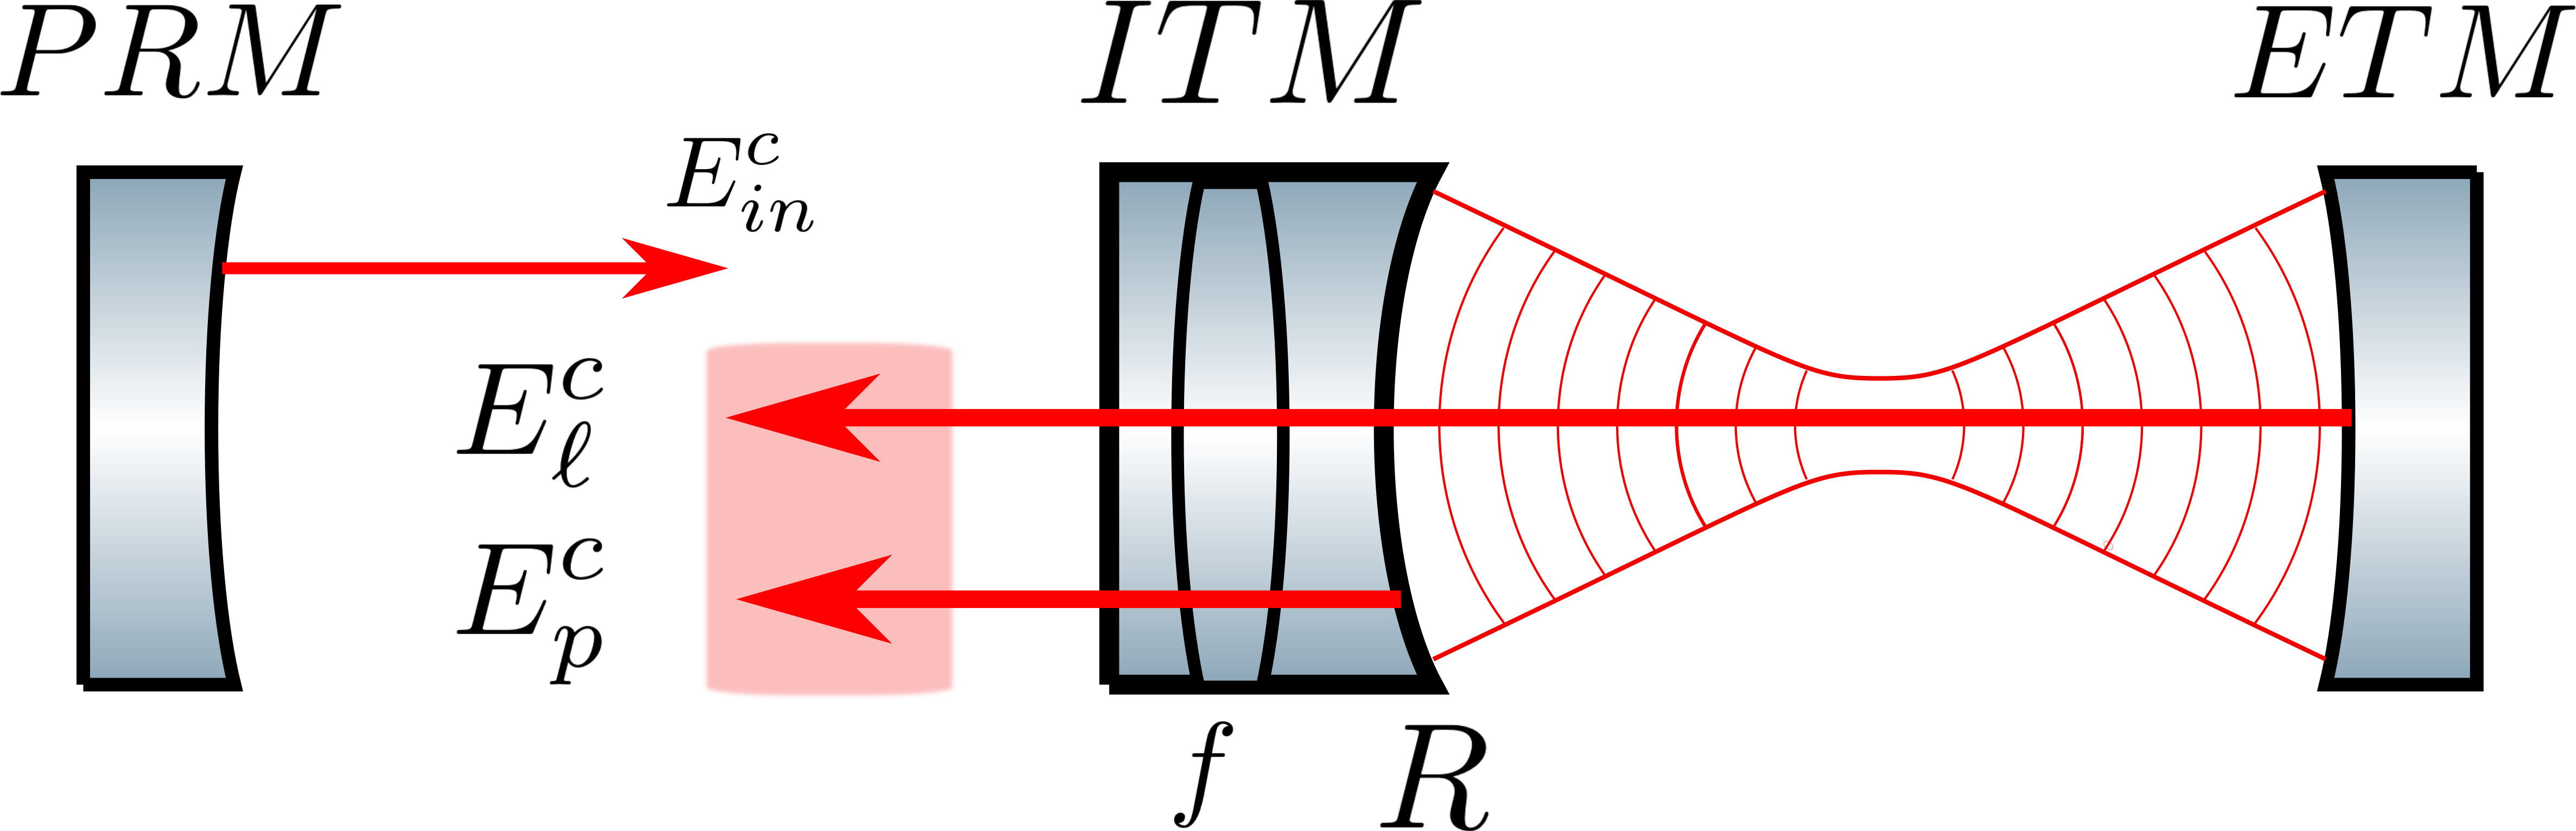
\includegraphics[width=.7 \textwidth]{../Figures/ThermalLensFP.png}
		\caption[A simplified model for the effect of a substrate thermal lens on the carrier field.]  
		{\textbf{A simplified model for the effect of a substrate thermal lens on the carrier field.} An input beam, $E_{\text{in}}^{c}$, from the power recycling mirror (PRM) will have a radius of curvature that mode matches to the input test mass (ITM).  The promptly reflected beam, $E_{p}^{c}$, is denoted by equation \ref{eq:promptE} and the leakage beam, $E_{\ell}^{c}$, is expressed by equation \ref{eq:leakE} where the sum of them would make the total reflected beam.  The leakage field will have the same shape as the ITM radius of curvature $R$ when exiting the arm and see the thermal lensing $f$. The promptly reflected field will also see the lens $f$ twice but when combined with the leakage beam, the \textit{total} reflected field is not affected by the thermal lens.}
		\label{fig:ThermalLensFP}
	\end{figure}
		\subsubsection{Carrier}\label{Sec:carrier_lensing}
		The carrier is resonant in the 4 kilometer arm cavities as well as the PRC, so a simplified model resembles a coupled cavity setup where there is already a locked resonator with some leakage beam and there is an input mode propagating from the power recycling cavity.  Consider the diagram in Figure \ref{fig:ThermalLensFP}, which shows a two-mirror optical system with an input carrier beam, $\ket{E^c_{\text{in}}}$, that has a portion promptly reflected off the input mirror to create $\ket{E^c_{p}}$
		\begin{equation}
		\ket{E^{c}_{p}} = \hat{M}^{c}_{p} \ket{E^{c}_{\text{in}}}
		\end{equation}
		The prompt reflection is made up of a beam incident on a converging lens from the substrate and a single reflection from the input coupler's convex surface, therefore, the transfer matrix is
		\begin{equation}
		\hat{M}^{c}_{p} = 
		\begin{bmatrix}
						1 	&	0 
		\\ 	-\frac{1}{f} 	&	1
		\end{bmatrix}
		\begin{bmatrix}
						1 	&	0 
		\\ 	+\frac{2}{R} 	&	1
		\end{bmatrix}
		\begin{bmatrix}
						1 	&	0 
		\\ 	-\frac{1}{f} 	&	1
		\end{bmatrix}
		\end{equation}
		where $R$ is the radius of curvature of the high reflectivity (HR) surface and $f$ is the thermal lens of the mirror substrate. In general, this can be a combination of the static lens and any thermal effects which create additional (intentional or non-intentional) lensing.
		
		\begin{equation}\label{eq:promptE}
		 \ket{E^{c}_{p}}=
		 \hat{M}^{c}_{p}
		 \begin{bmatrix}
		 					1  
		 \\ 	\frac{1}{q_{\text{in}}}
		 \end{bmatrix}
		 =
		 \begin{bmatrix}
		 1  
		 \\ 	\frac{1}{q_{\text{in}}} + 2 \big(\frac{1}{R} - \frac{1}{f}\big)
		 \end{bmatrix}
		 =
		 \begin{bmatrix}
		 1  
		 \\ 	\frac{1}{q_{\text{p}}}
		 \end{bmatrix}
		\end{equation}
		Here, $\frac{1}{q_{\text{in}}} = -\frac{1}{R_{\text{in}}} - i \frac{\lambda}{\pi w^2}$, is the q-parameter of the input beam where $w$ is the beam size on the HR surface and $R_{\text{in}}$ is the radius of curvature entering the cavity and is converging at that point.
		
		In addition, there is also a circulating field inside the cavity which leaks out in reflection and can be denoted by $\ket{E^c_{\ell}}$ which exits with the input coupler's radius of curvature and sees a single pass through the substrate lens,
		\begin{equation}\label{eq:leakE}
		\ket{E^c_{\ell}} = 		 
		\begin{bmatrix}
		1 	&	0 
		\\ 	-\frac{1}{f} 	&	1
		\end{bmatrix}
		\begin{bmatrix}
		1  
		\\ 	\frac{1}{R} - i\frac{\lambda}{\pi w^2}
		\end{bmatrix}
		=
		\begin{bmatrix}
		1  
		\\ 	\frac{1}{R} -i\frac{\lambda}{\pi w^2} - \frac{1}{f}
		\end{bmatrix}
		\end{equation}
		The total reflected beam is a summation of the prompt and leaked cavity fields.  LIGO uses arms which are highly over-coupled optical cavities so the promptly reflected amplitude is $\vert E^c_p \vert \approx \vert E_{\text{in}} \vert$ and using equation \ref{c_FP}, the leakage amplitude is $\vert E^c_\ell \vert \approx -2\vert E_{\text{in}} \vert$.  Putting all this together, the total reflected field of the carrier is
		\begin{equation}
		\begin{aligned}
		E^c_{\text{REFL}} 	&= E^c_{\ell} + E^c_p \\
							&= E_{\text{in}} \bigg[ \exp \bigg(\frac{-ik r^2}{2q_p}\bigg) - 2  \text{exp} \bigg(\frac{-ik r^2}{2q_{\ell}}\bigg) \bigg]\\
							&\approx E_{\text{in}} \bigg[ -1 - \frac{ikr^2}{2} \bigg( \frac{1}{q_p} - \frac{2}{q_\ell} \bigg) \bigg]\\
							&\approx E_{\text{in}} \bigg[ -1 - \frac{ikr^2}{2} \bigg[ \frac{1}{q_\text{in}} + \frac{2}{R} - \frac{2}{f}  - 2 \bigg(\frac{1}{R} - i\frac{\lambda}{\pi w^2} - \frac{1}{f} \bigg) \bigg] \bigg]\\
							&\approx -E_{\text{in}} \bigg[ 1 + \frac{ikr^2}{2} \bigg[ -\frac{1}{R_\text{in}} + i\frac{\lambda}{\pi w^2}  \bigg] \bigg]\\
							&\approx -E_{\text{in}} \exp\bigg(\frac{-ikr^2}{2} \bigg[ \frac{1}{R_{\text{in}}} - i\frac{\lambda}{\pi w^2}  \bigg]\bigg) 
		\end{aligned} 
		\end{equation}
		The fourth line is where the phase gain due to the substrate thermal lens and test mass radius of curvature will cancel for the prompt reflection and the leakage beams. The last line shows that the total reflected carrier field will be negative of the original amplitude with the same beam size and absolute curvature, however, now the beam is diverging instead of converging.  \textbf{The amazing part is that the end result is independent of the substrate lensing to first order}.  Here, the approximation used to expand the exponential from the second to the third line is valid when considering points close to the beam center ($\frac{k r^2}{R}<<1$) where the paraxial approximation is true \cite{Saleh}.  If considering areas where this condition is not strictly true, the model is only meant to show that the first leading order term between the leakage and promptly reflected fields cancel, which will \textbf{not} be true for second order effects.  Another point where this model breaks down is when the power recycling mode is altered so much by lensing effects that the PRC is no longer well mode matched to the arms; this leads to the input beam not having the right radius of curvature.  At that point, there will be extra losses from higher order mode-coupling.  Lensing can also change the radius of curvature to a point where the PRC g-factor makes the resonant mode no longer geometrically stable (see Appendix \ref{FPappendix}), however, this requires significant thermal lensing well beyond what is expected in Advanced LIGO \cite{Lawrence_TCS}.  A numerical FINESSE model uses this simplified geometry to calculate the power recycling gain and arm build up in Figure \ref{fig:simple_prc_arm} as a function of round trip losses and thermal lensing.
		\subsubsection{Sidebands}
		Using the same formalism as the carrier fields, the sidebands will have the same input curvature, however, they do not resonate in the arms so there is no cavity leakage field.  Therefore, the sidebands will see the phase change due to the substrate lens and this has very important consequences on the sideband build up within the power recycling cavity.
		\subsubsection{GW Signal}
		As mentioned in Section \ref{sec:DRMI}, LIGO currently employs a DC readout scheme that extracts the signal by beating the carrier field with the audio frequency sidebands created by the gravitational wave.  Although the carrier field was shown to be immune from substrate thermal lensing, the gravitational wave sideband field will see a single-passed lensing effect as it propagates out of the cavity and towards the beamsplitter.  If there is differential lensing, the signal recycling cavity will see an effective thermal lens, $\text{TL}_{-}$, which will scatter light into higher order modes.  This causes a reduction in the amount of gravitational wave signal at the anti-symmetric port that is directly proportional to the mode mismatch between the arms.
		
	\section{Wavefront Distortions from Thermal Effects}\label{sec:wf_dist}
	In the previous section, it was shown that lensing in the substrate affects fields in the interferometer differently.  The thermal distortions were modeled as a simple addition of phase, however, it is useful to understand how the optical path varies from first principles.  This provides theoretical groundwork for modeling interferometer heating as well as corrective measures using TCS.  A lot of work in this field was introduced in the context of gravitational wave detectors by Hello and Vinet \cite{hello_vinet} \cite{Vinet_Thermal_Issues} where they implemented the Heat Diffusion equation in order to analytically derive the phase change due to thermal aberrations.  In general, there are two effects which occur when a beam interacts with an optic which has a temperature field: thermo-refractive and thermo-elastic.  
	
	The first arises from the index of refraction changing as a function of the temperature distribution $T(r,z)$,
	\begin{equation}
	\Delta n_{r}(r,z) = \frac{\text{d}n}{\text{d}T} \, T(r,z)
	\end{equation}
	where $\frac{\text{d}n}{\text{d}T}$ is the temperature index coefficient and is dependent on the optic material, which can be (and often is) inhomogeneous.  For example, if the heating source comes from a laser beam which imparts onto the optic a Gaussian-like intensity pattern, inhomogeneities in the optic cause the temperature profile to be non-uniform and thus leading to a varying index of refraction that causes wavefront distortions (see Figure \ref{fig:ThermalLensWF}).
	
	\begin{figure}[ht!]
		\centering
		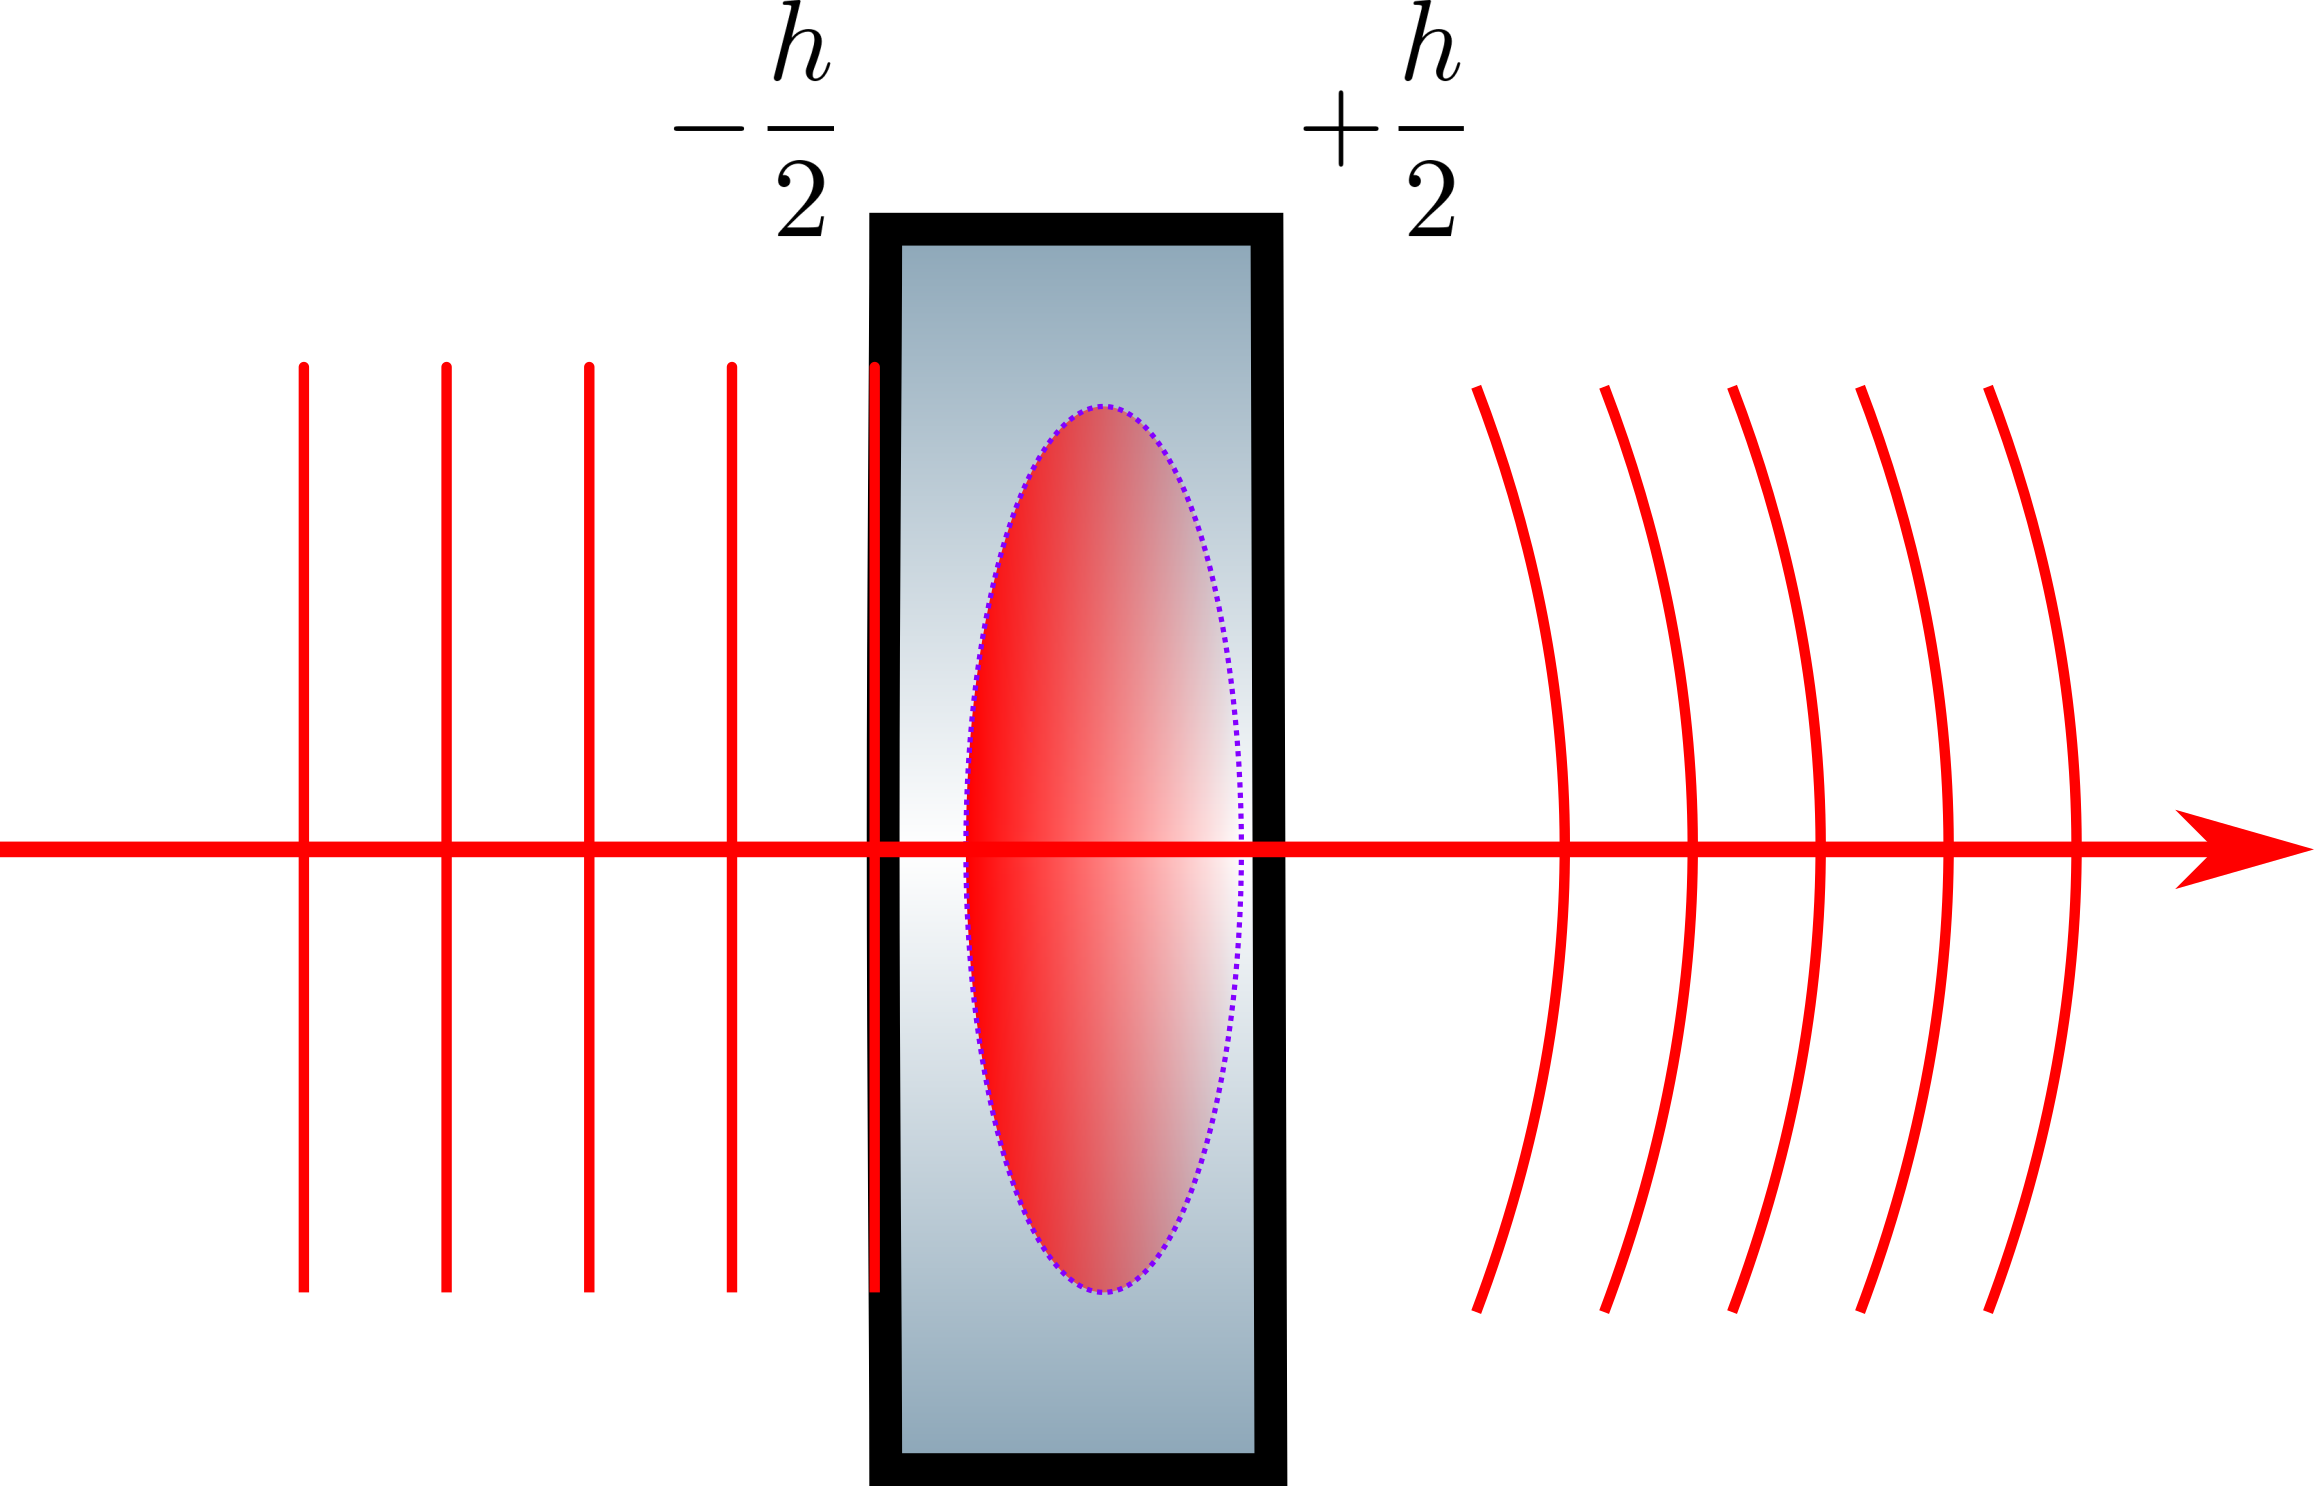
\includegraphics[width=.4 \textwidth]{../Figures/ThermalLensWF.png}
		\caption[A plane wave passing through a lens with a temperature gradient.]  
		{\textbf{A plane wave passing through a lens with a temperature gradient.} The index of refraction, $n$, depends on the material and temperature so when a plane wave moves through a medium with a non-uniform temperature field, a phase lag or lead occurs in the wavefront. Since $\frac{\text{d}n}{\text{d}T}$ is negative, the distortion will resemble a diverging lens.}
		\label{fig:ThermalLensWF}
	\end{figure}

	To understand how changing the index of refraction varies the optical path length, consider the function $S(r)$ which describes surfaces that are perpendicular to the rays. If $S(r)$ is a known function then the rays can be reconstructed using the gradient, $\nabla S(r)$.  As an analogy to electrostatics, $S(r)$ is similar to the potential function $V$ and the electric field is described by $\bf{E}=-\nabla V$.  As an extension of ray optics, Fermat's principle requires that the Eikonal equation be satisfied,
	\begin{equation}
	\vert \nabla S \vert^2 = n^2
	\end{equation}
	By integrating along the axis of propagation ($\hat{z}$) in Figure \ref{fig:ThermalLensWF} through the substrate, one can find the optical path distortion
	\begin{equation}\label{eq:thermoref}
	Z(r) =  \frac{\text{d}n}{\text{d}T} \int_{-h/2}^{+h/2} \, T(r,z) \text{d}z
	\end{equation}
	It is clear that the temperature field is key to understanding exactly how the wavefront is distorted. In order to analytically solve for $T(r,z)$, one must invoke the famous Heat equation,
	\begin{equation}\label{eq:heat_eq}
		\kappa \nabla^2 T(r,z) = \rho C\, \frac{\partial T}{\partial t} 
	\end{equation}
	where $\kappa$ is the thermal conductivity, $\rho$ is the density, and $C$ is the specific heat.  A complete solution for such an equation will be a sum of two parts: 
	\begin{equation}
	T(r,z,t) = T_{s}(r,z) + T_{t}(r,z,t)
	\end{equation} 
	where the first term is the steady-state solution which includes the an ambient temperature and a perturbation, $T_s(r,z) = T_p(r,z) + T_0$.  The main goal for the remainder of the section will be finding a solution to the perturbation field.  The second term is the transient time-dependent solution which will converge to the stead-state as time goes to infinity.  For the LIGO test masses which are approximately cylindrical, the heat equation in steady-state equilibrium is
	\begin{equation}
		\kappa \bigg[ \frac{1}{r} \frac{\partial}{\partial r} \bigg( r \frac{\partial}{\partial r}\bigg) +  \frac{\partial^2}{\partial z^2} \bigg] T_s(r,z) = 0
	\end{equation}
	The next step is to understand the boundary conditions using Figure \ref{fig:ThermalLensFlux} and the balance of heat fluxes at each of the surfaces,
	\begin{equation}
	\textbf{n} \cdot [ \textbf{F} + \kappa \nabla T_s]_{\text{surf}} = 0 
	\end{equation}
	Assuming that the outward flux is from radiation which follows the Stefan-Boltzmann law,
	\begin{equation}\label{eq:heat_flux}
	\begin{aligned}
	[\textbf{n} \cdot  \textbf{F}]_{\text{surf}} = \sigma_B  [T_s^4 - T_0^4] 	&= \sigma_B [(T_p(r,z) + T_0)^4 - T_0^4] \\
																			&\approx 4 \sigma_B T_0^3 T_p(r,z)
	\end{aligned}
	\end{equation}
	where $\sigma_B$ is the Stefan-Bolzmann's constant.  It is important to note that $\sigma_B$ depends on the material and may vary by a scalar amount but for brevity, it is used as a constant here.  The last part of the equation assumes that the temperature field is only a small perturbation from the ambient surroundings, $T_p(r,z) << T_0$, which allows the radiation term to become linear.  Figure \ref{fig:ThermalLensFlux} shows boundary conditions for the LIGO test masses,
	
	\begin{figure}[ht!]
		\centering
		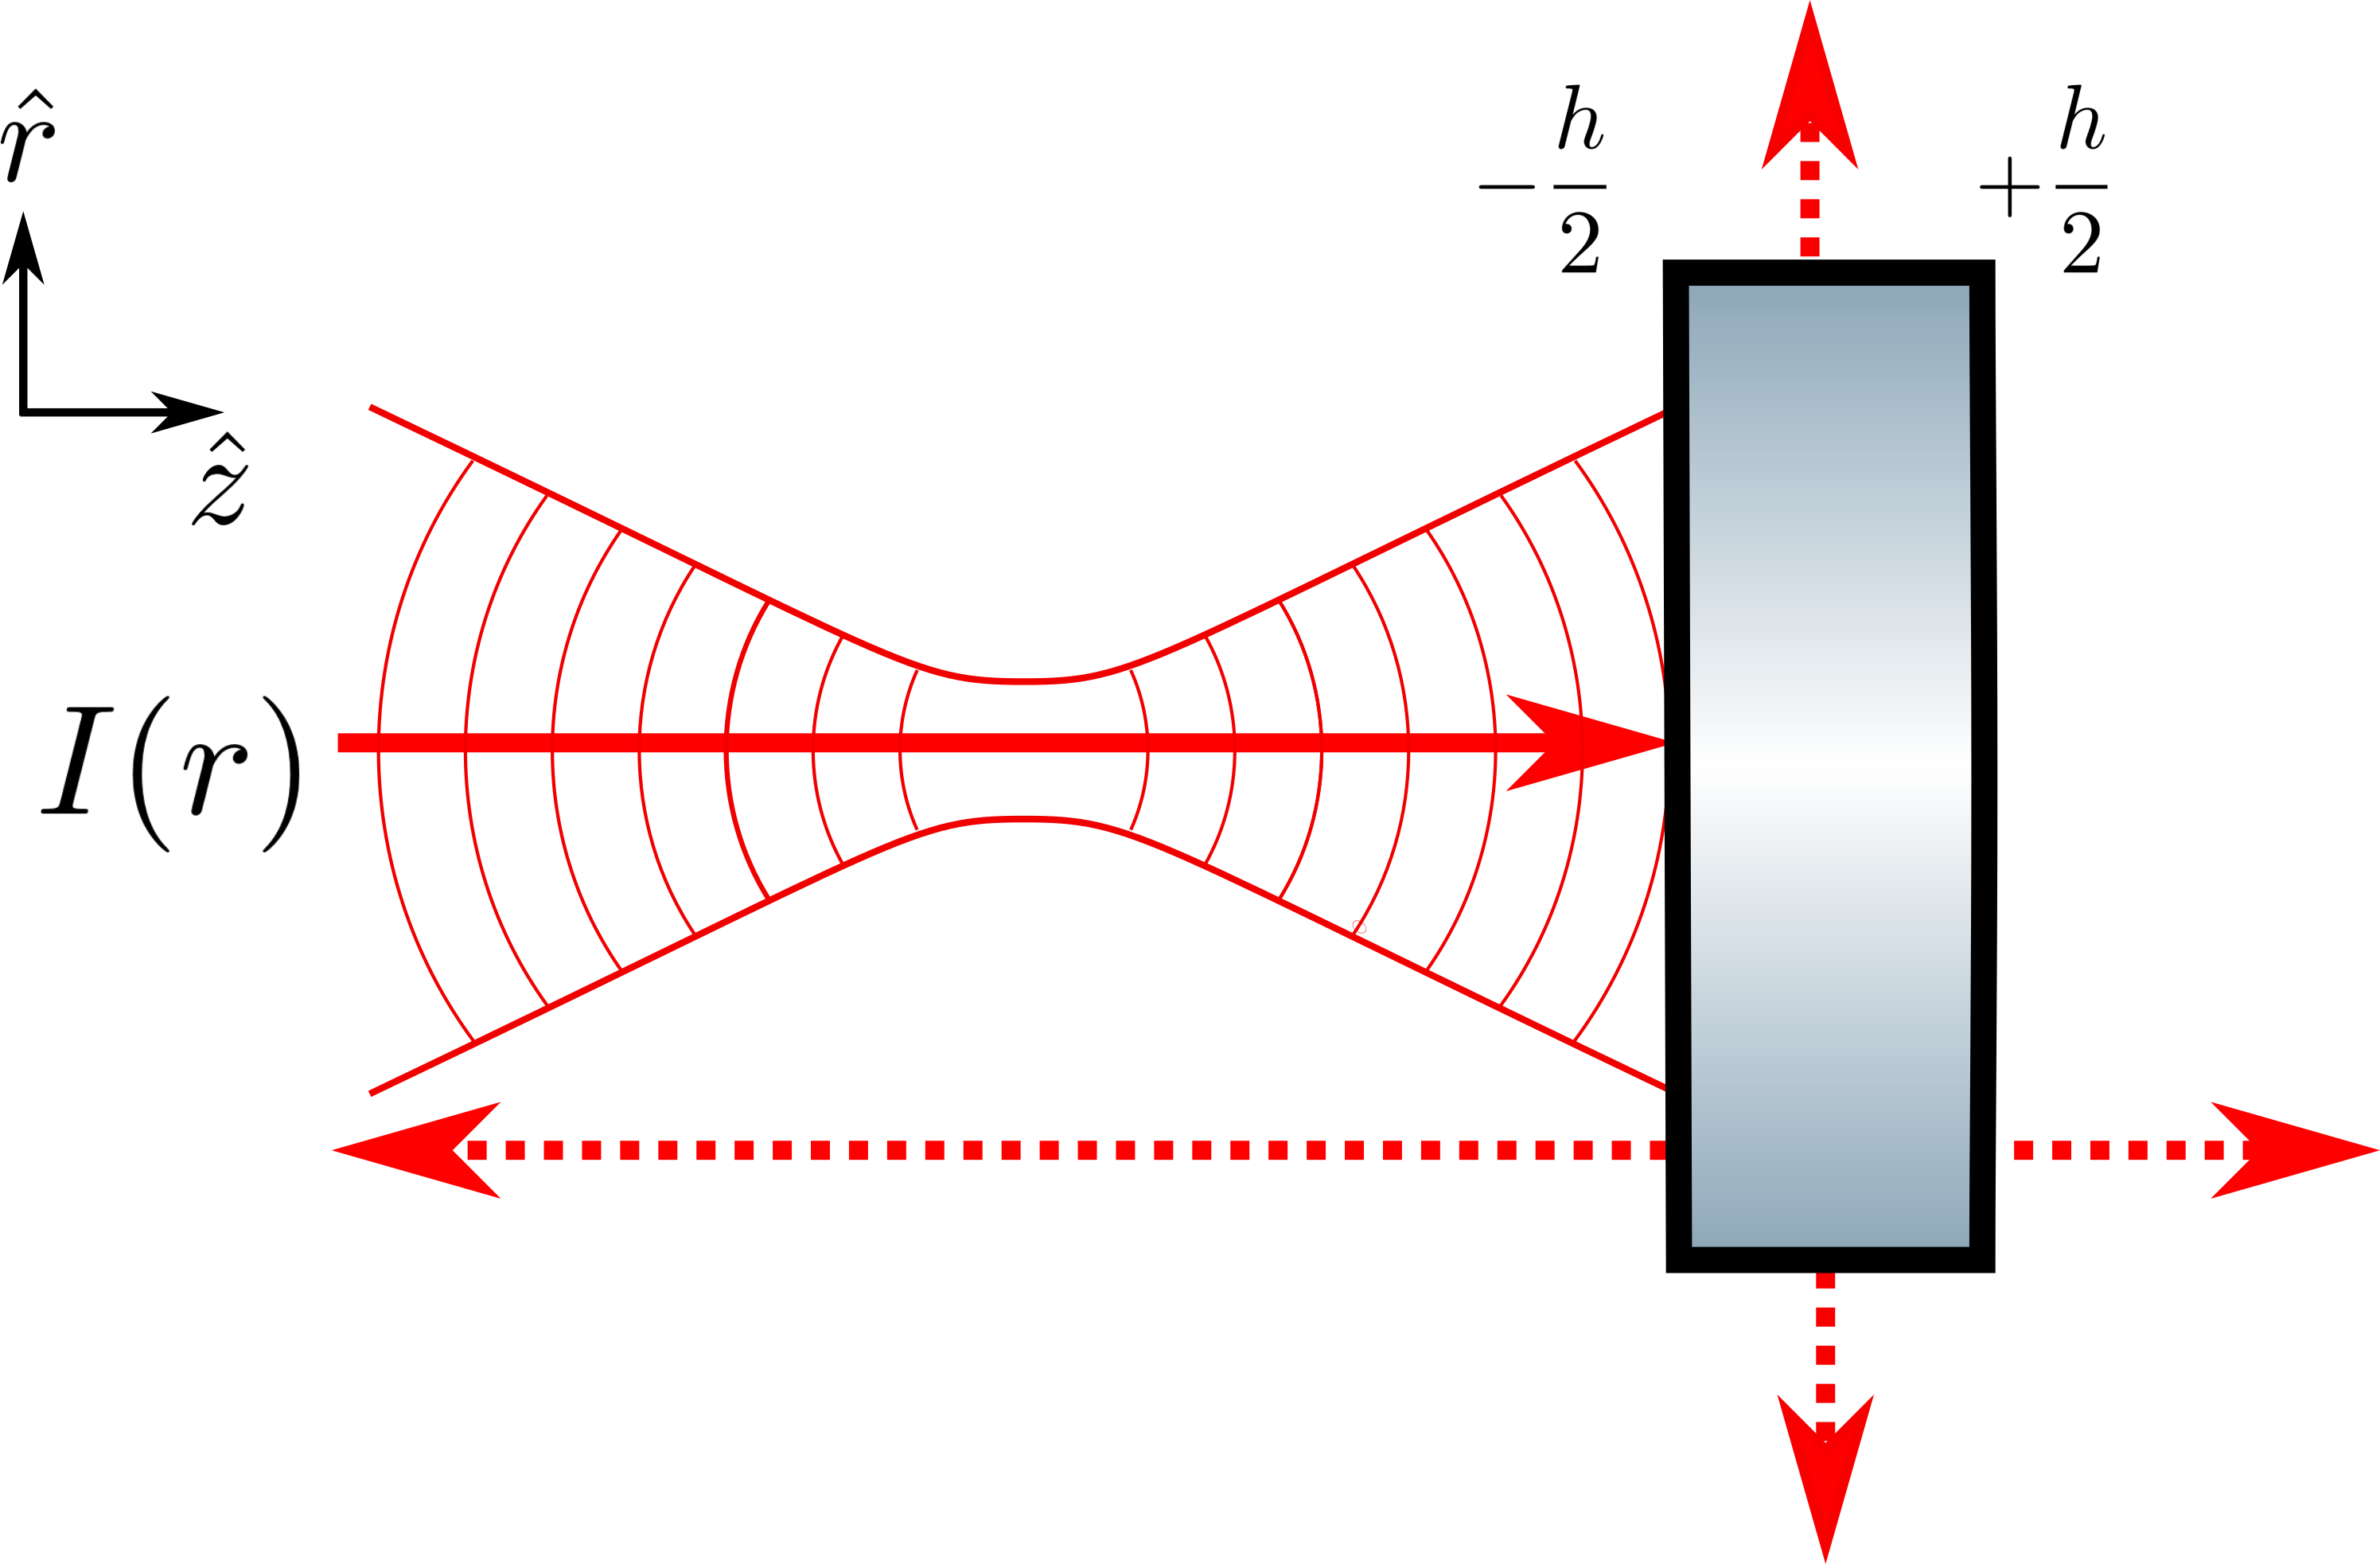
\includegraphics[width=.6 \textwidth]{../Figures/ThermalLensFlux.png}
		\caption[A conceptual model of flux balance for a cylindrical object.]  
		{\textbf{A conceptual model of flux balance for a cylindrical object.} The red dotted lines represent the radiative fluxes escaping the optic while a Gaussian beam with intensity profile $I(r)$ is pumping energy in as denoted by the red solid line.}
		\label{fig:ThermalLensFlux}
	\end{figure}

	At the surface where $z=h/2$ the total flux is radiative,
	\begin{equation}\label{eq:faceh2}
	-\kappa \frac{\partial T_p(r,h/2)}{\partial z} = 4 \sigma_B T_0^3 T_p(r,h/s)
	\end{equation}
	
	At the barrel of the cylinder where $r=a$, total flux is also radiative,
	\begin{equation}\label{eq:barrel}
	-\kappa \frac{\partial T_p(a,z)}{\partial r} = 4 \sigma_B  T_0^3 T_p(a,z)
	\end{equation}
	
	At the surface where $z=-h/2$ there are two components of flux, one is radiative and the second is the input power from the laser beam striking the optic surface,
	\begin{equation}\label{eq:face-h2}
		-\kappa \frac{\partial T_p(r,-h/2)}{\partial z} =  -4 \sigma_B T_0^3 T_p(r,-h/s) + \epsilon_a I(r)
	\end{equation}
	where $I(r) = \frac{2P}{\pi w^2} \exp{-2r^2/w^2}$ is the laser beam intensity with power $P$ over a beam size of $w$ and $\epsilon_a$ is the absorption coefficient.  Here, the radiative term has a negative sign to represent the flux direction. Once boundary conditions are established,  most introductory textbooks that deal with partial differential equations will apply an educated guess for the solution.  In this case, the resulting temperature field will be a harmonic function,
	\begin{equation}
	T_p(r,\phi,z) =  (A e^{+k z} + B e^{-kz}) J_0(kr)
	\end{equation}
	where $J_0$ is the spherical Bessel function of the first kind and $k$ is a constant.  Although this particular temperature distribution can be even more general by allowing all the orders of $J_n$, this form is sufficient. Using the boundary condition from \ref{eq:barrel} and the property $\frac{\partial J_0(x)}{\partial x} = -J_1(x)$,
	\begin{equation}
		-\kappa k \frac{\partial J_0(kr)}{\partial r} \bigg\vert_{r=a} = 4 \sigma_B T_0^3 J_0(ka)
	\end{equation}
	\begin{equation}\label{eq:sphere_bessel}
		ka J_1(ka) - \chi J_0(ka)=0
	\end{equation}
	where $\chi = 4\sigma T_0^3 a/\kappa$ is the reduced time constant.  There exists an infinite number of discrete solutions which can solve \ref{eq:sphere_bessel} using various values of $k_n a = \rho_n$.
	The temperature field then becomes,
	\begin{equation}\label{eq:temp2}
	T_p(r,z) = \sum_{n=0}^{\infty} (A_n e^{+k_n z} + B_n e^{-k_n z}) J_0(k_n r)
	\end{equation}
	In order to solve the conditions from equations \ref{eq:faceh2} and \ref{eq:face-h2}, the strategy is use the orthogonality of the spherical Bessel functions in order to expand the equations into a solvable algebraic form.  This will include expanding the intensity profile $I(r)$ in this basis as well.  Consider the boundary from $r=0$ to $r=a$, the functions $J_0(k_n r)$ form a complete basis set and the normalization constant is given by the Sturm-Louisville problem,
	\begin{equation}
	\int_{0}^{a} J_0(k_n r) J_0(k_m r) \,r \, \text{d}r= \delta_{mn} \frac{[\chi^2 + (k_na)^2]}{2k_n^2} J^2_0(k_na) = \delta_{mn} \frac{1}{N_n}
	\end{equation}
	Then expanding the intensity profile in terms of the Bessel function: $I(r)= \sum_{n}^{\infty} p_n J_0(k_n r)$ and inverting to solve for $p_n$ leads to,
	\begin{equation}
	\begin{aligned}\label{eq:p_n_gauss}
	p_n &= N_n \int_{0}^{a} I(r) J_0(k_n a) \, r \, \text{d}r\\
		&= N_n \int_{0}^{a} \bigg[\frac{2 P}{\pi w^2}\bigg] J_0(k_n a) \exp{-2r^2/w^2} \, r \, \text{d}r\\
		&\approx N_n \, \frac{P}{2\pi a^2} \, \exp{-\frac{(k_n w )^2}{8} } 
	\end{aligned}
	\end{equation}
	The approximation came from integrating to infinity instead of $a$ which is reasonable if diffraction losses are small on the substrate.  Plugging in the equation \ref{eq:temp2} and $I(r)$ into the remaining boundary conditions,
	\begin{subequations}
		\begin{equation}
		\bigg[ k_n - \frac{4\sigma_B T_0^3}{\kappa}\bigg] e^{-k_nh} A _n - \bigg[ k_n + \frac{4\sigma_B T_0^3}{\kappa}\bigg] B_n = \frac{\epsilon p_n  }{\kappa} e^{-k_nh/2}
		\end{equation}
		\begin{equation}
		\bigg[ k_n + \frac{4\sigma_B T_0^3}{\kappa} \bigg] A _n - \bigg[ k_n - \frac{4\sigma_B T_0^3}{\kappa}\bigg] B_n e^{-k_nh} = 0
		\end{equation}
	\end{subequations}
	Solving for $A_n$ and $B_n$,
	\begin{subequations}
		\begin{equation}
			A_n = \frac{\epsilon_a p_n}{\kappa} e^{-3k_n h /2} \frac{\eta_{+}}{\eta_{+} - \eta_{-} e^{-2k_n h} }
		\end{equation}
		\begin{equation}
			B_n = \frac{\epsilon_a p_n}{\kappa} e^{-k_n h /2} \frac{\eta_{-}}{\eta_{+} - \eta_{-} e^{-2k_n h} }
		\end{equation}
	\end{subequations}
	where $\eta_{\pm} = k_n \pm \frac{4\sigma_B T_0^3}{\kappa}$ is used for brevity. Now it is possible to write down the entire steady-state temperature field for a cylindrical test mass with a laser beam impinging on the surface,
	\begin{equation}
	T_p(r,z) = \sum_{n=0}^{\infty} \frac{\epsilon_a p_n}{\kappa}  \; \frac{ \eta_{-}e^{-k_n(3h/2-z)} + \eta_{+}e^{-k_n(h/2-z)}  }{\eta_{+} - \eta_{-} e^{-2k_n h} } J_0(k_n r)
	\end{equation} 
	Once the temperature profile is solved, the path length distortion from the thermo-refractive effect can be found by solving by equation \ref{eq:thermoref},
	\begin{equation}
	Z_{\text{TR}}(r) = \frac{\text{d}n}{\text{d}t} \frac{\epsilon_a}{\kappa} \sum_{n=0}^{\infty} \, \frac{p_n}{k_n} \, \frac{1- e^{-k_n h}}{[\eta_{+} - \eta_{-} e^{-k_nh}]} \; J_0(k_n r) 
	\end{equation}
	where $p_n$ contains information about the heating profile so it is possible to directly plug in equation \ref{eq:p_n_gauss} to represent the distortion from a Gaussian beam,
	\begin{equation}
	Z_{\text{TR}}^{G}(r) =  \frac{\text{d}n}{\text{d}t} \frac{\epsilon_a \, P}{2\pi a^2 \kappa} \sum_{n=0}^{\infty} \, \frac{N_n}{k_n}\, e^{-(k_n w)^2/8} \, \frac{1- e^{-k_n h}}{[\eta_{+} - \eta_{-} e^{-k_nh}]} \; J_0(k_n r) 
	\end{equation}
	The thermo-refractive effect due to coating and substrate absorption is only one type, there is also an effect which elastically curves the surface from thermal expansion \cite{Vinet_Thermal_Issues}.  This thermo-elastic effect deals with the internal stresses of the material and employs the stress-strain relations in order to derive the wavefront curvature.  For the LIGO test masses which use fused silica, this effect is smaller than the thermo-refractive wavefront distortion by about an order of magnitude.
	
	\section{Contrast Defect}
	Generally, the contrast defect is defined as the ratio of the darkest to the brightest power at a given point in the interferometer, which in practice is the ratio of power at the antisymmetric and reflected port when locked on a dark fringe.  In other words, it is the amount of junk light that is present in the interferometer when light between the two arms do not perfectly interfere with each other. This junk light can be the symptom of various causes, for example, an imbalance of reflectivity between ITMX and ITMY will cause non-perfect destructive interference at the antisymmetric port and a camera would see a TEM00 beam when locked on length.  Another cause of contrast defect could be from misalignment between the ITMs or beamsplitter which will result in seeing a TEM 01/10 mode.  However, if both of the aforementioned causes are fixed with a combination of stringent design specifications for the reflectivity and alignment loops closed to minimize angular jitter, then the contrast defect will be dominated by mode mismatch which can be fixed by a combination of ring heaters and CO$_2$ lasers.  The picture gets even more complicated when adding in the absorption for individual optics and introducing multiple Fabry-Perot cavities which will treat the sidebands and carrier fields differently.  
	
	One of the main goals for the Thermal Compensation System is to correct the cold and hot interferometer differences in radii of curvature.
	
	\subsection{Simple Michelson Contrast Defect}
	The simple Michelson can give a first estimate of the contrast defect when starting to commission the interferometer's thermal system, however, it is not used in nominal low noise since the dual-recycled Michelson is implemented.  By propagating the input mode cleaner beam to the beamsplitter and taking a single bounce at the high reflectivity surface, one can approximate the resultant mode overlap by measuring the power at the antisymmetric port.  The static mismatch correction was measured this way and is compensated using one of the CO$_2$ lasers to reduce the contrast at 2 Watts of input power from $0.4\%$ to $0.1\%$.
	
	At this point the carrier and sideband fields follow the same ABCD matrix transfer function, so only one calculation is needed to estimate the contrast defect.  A keen reader will notice that this model will not take the Schnupp asymmetry into account which allows the $\hat{x}$-direction beam to travel an extra 8 centimeters further than the $\hat{y}$, however, this effect will only change the end result by approximately 10$\%$.  In fact, for this interferometer configuration, the dominate source of mismatch will be from the prompt reflection off the HR surfaces of the ITMs where most of the phase change occurs.  The sideband contribution at the antisymmetric port can be estimated by using equation \ref{sb_tf} and measuring the modulation depth, $\Gamma_{\Omega}$, for the 9 and 45 MHz RF fields that enter the interferometer,
	\begin{equation}
	\begin{aligned}
	P_{\text{SB}}	&= 2 P_{\text{in}} \bigg( \frac{\Gamma}{2} \bigg)^2 t_{SB\pm} \\
	&= 2 P_{\text{in}} \bigg( \frac{\Gamma}{2} \bigg)^2 \sin^2(k_{\Omega} \Delta \ell)
	\end{aligned}
	\end{equation}
	Additionally, the beamsplitter RMS motion will also contribute extra power at the AS and can be estimated by calculating the coupling coefficient from the 00 to 01 HG mode,
	\begin{equation}
	P_{01} = 2 P_{\text{in}} \bigg( \frac{\pi \, \alpha \, w(z)}{\lambda}\bigg)^2
	\end{equation}
	where $w(z)$ is the beam size on the test mass and $\alpha$ is the misalignment RMS.
	
	\subsection{Modal Contrast Defect}
	During full lock, the formalism must be extended to include the mode shape of two arm cavities interfering at the beamsplitter. Using the Laguerre-Gauss modes is useful for brevity because the mode mismatch couples to only one higher order mode. Contrast defect can be defined using the zeroth eigenmode of each arm and then expanded to project the X-arm's basis onto Y-arm using higher order LG modes, $LG^{00}_y \rightarrow  LG^{00}_x + \alpha LG^{10}_x$.  Where $\alpha = \frac{1}{\sqrt{2}} \big(\frac{\Delta \omega_{0}}{\omega_{0}} + i \frac{\Delta z }{z_R}\big)$ is the amount of higher order mode coupling due to mismatch in beam size and location, respectively (see Chapter 3).
	\begin{equation}\label{CD_mode}
	\begin{aligned}
	\text{CD} 	&\equiv \frac{P_{AS}}{P_{REFL}} \\
	&= \frac{\vert LG^{00}_x - LG^{00}_y \vert^2}{\vert LG^{00}_x + LG^{00}_y \vert^2}\\
	&= \frac{\vert LG^{00}_x \vert^2 + \vert LG^{00}_x + \alpha LG^{10}_x \vert^2 - 2\Re(LG^{00}_x [LG^{00*}_x + \alpha LG^{10}_x ])}{\vert LG^{00}_x \vert^2 + \vert LG^{00}_x + \alpha LG^{10}_x \vert^2 + 2\Re(LG^{00}_x [LG^{00*}_x + \alpha LG^{10}_x ])}\\
	&\approx \frac{\alpha^2}{4}\\
	&\approx \frac{1}{8} \bigg[ \bigg(\frac{\Delta\omega_{0}}{\omega_{0}} \bigg)^2+  \bigg(\frac{ \Delta z }{z_R}\bigg)^2 \bigg]
	\end{aligned}
	\end{equation}
	Mismatch between the arm cavities can stem from a few sources such as the difference between the radii of curvature on the high reflectivity surfaces that will cause the resonant modes to be shaped differently between the X-arm and Y-arm. LIGO tries to optimize this effect by pairing the optics based on their properties, however, during the upgrades from O2 to O3 at Hanford, ITMX was replaced but ITMY was not which lead to a static mismatch between the input test masses.
	
	\section{Tuning Thermal Compensation for LIGO}
	
	As mentioned in Section \ref{Sec:TL_lensing}, the circulating power in each of the arms can be close to 150 kW for O3 and will be higher for the subsequent observation runs.  Even with absorption only in the range of $0.2-0.8$ parts per million, the induced substrate lensing can be significant.  The Thermal Compensation System (TCS) \cite{Lawrence_TCS} \cite{AWC_current} \cite{winkler_thermaldist} \cite{Strain_TL} was developed to correct the wavefront by applying heat to cancel the deformities caused by interferometer heating.  Ease of lock acquisition and gravitational-wave noise minimization are the main criteria for success when commissioning most LIGO systems.  To aid in the former, TCS is required to thermally lens the ITM substrate such that the optical path difference is minimized for the carrier and sideband power recycling gains.
	
	To optimize the TCS settings for the best power build-ups, there are two separate strategies:  The first requires estimating the amount of absorption on the test masses with the Hartmann Wavefront Sensors to measure the optical path distortion induced by the interferometer during a lock loss.  Then pre-load the ring heaters with the nominal settings which would cancel carrier beam's thermal absorption in the ``hot" state.  The ring heaters have a very long time constant (30 hours) to reach thermal equilibrium with a step response of electrical power, so if there is compensation needed, the heaters must be energized at all times.    However, turning them on will change the radius of curvature and induce a substrate lens (see Section \ref{Sec:RH}) that has to be canceled out by the CO$_2$ (Carbon Dioxide) lasers which create a lens on the compensation plate of the quadruple pendulum.  Since the CO$_2$ lasers have a time constant of approximately 0.5 hours, they can be turned up during lock acquisition and reduced as needed when the interferometer input power is increased.
	
	The second method is to use relevant interferometer RF signals at various ports to experimentally adjust the lensing commonly or differentially to maintain power recycling build-ups while increasing the interferometer input power.  In principle, either method should lead to the same answer but in practice, both are used to find the nominal thermal compensation configuration.  The section below describes how to tune the Hartmann Sensors and how the system can be used to determine the uniform absorption. 
	\subsection{Hartmann Wavefront Sensors}\label{Sec:HWS}
	All estimates of steady-state curvature changes due to heating by the main interferometer beam depend linearly on the absorption. This can be quite difficult to detect when the coating absorption are typically less than one part in a million.
	
	In order to diagnose this effect, the Hartmann Wavefront Sensors (HWS) \cite{Brooks_OffAxis} \cite{Veitch_HWS_ALIGO} was developed by Adelaide and Caltech \cite{Brooks_HWS_2007} \cite{Brooks_HWS_2009}. It uses an auxiliary beams and charged-coupled imaging devices (CCD) to sense the wavefront distortions formed by heating from the interferometer beam during power up and a lock loss.  Currently, there are four Hartmann sensors installed at each test mass, which are injected from the AR surface side of the optics. Technical constraints require the ITM HWSs optical paths to differ from the ETM HWSs but the concept is still the same, so for brevity, only the ITMs HWSs will be discussed in detail.  In Figure \ref{fig:HWS_optical}, the system starts with an auxiliary super-luminous LED (SLED) beam being injected into the vacuum system and a telescope (Lens 1, Lens 2) which collimates/expands the beam to sample a space 200 mm in diameter on the test mass HR surface.  The return beams are picked-off and sent to a CCD with a Hartmann plate mounted on the front which effectively decompose the wavefront into individual rays.  Using a wavefront from a previous time with a cold optic as a reference. The Hartmann code creates a gradient vector field between the two times which have information about thermal lensing. Then numerically integrates the gradients to fit a wavefront field which is normally referred to as the optical path distortion in length units.  The algorithm then uses the Zernike polynomials as a single basis to represent the effective thermal lens. \cite{Brooks_thesis}
	
	\begin{figure}[!]
		\centering
		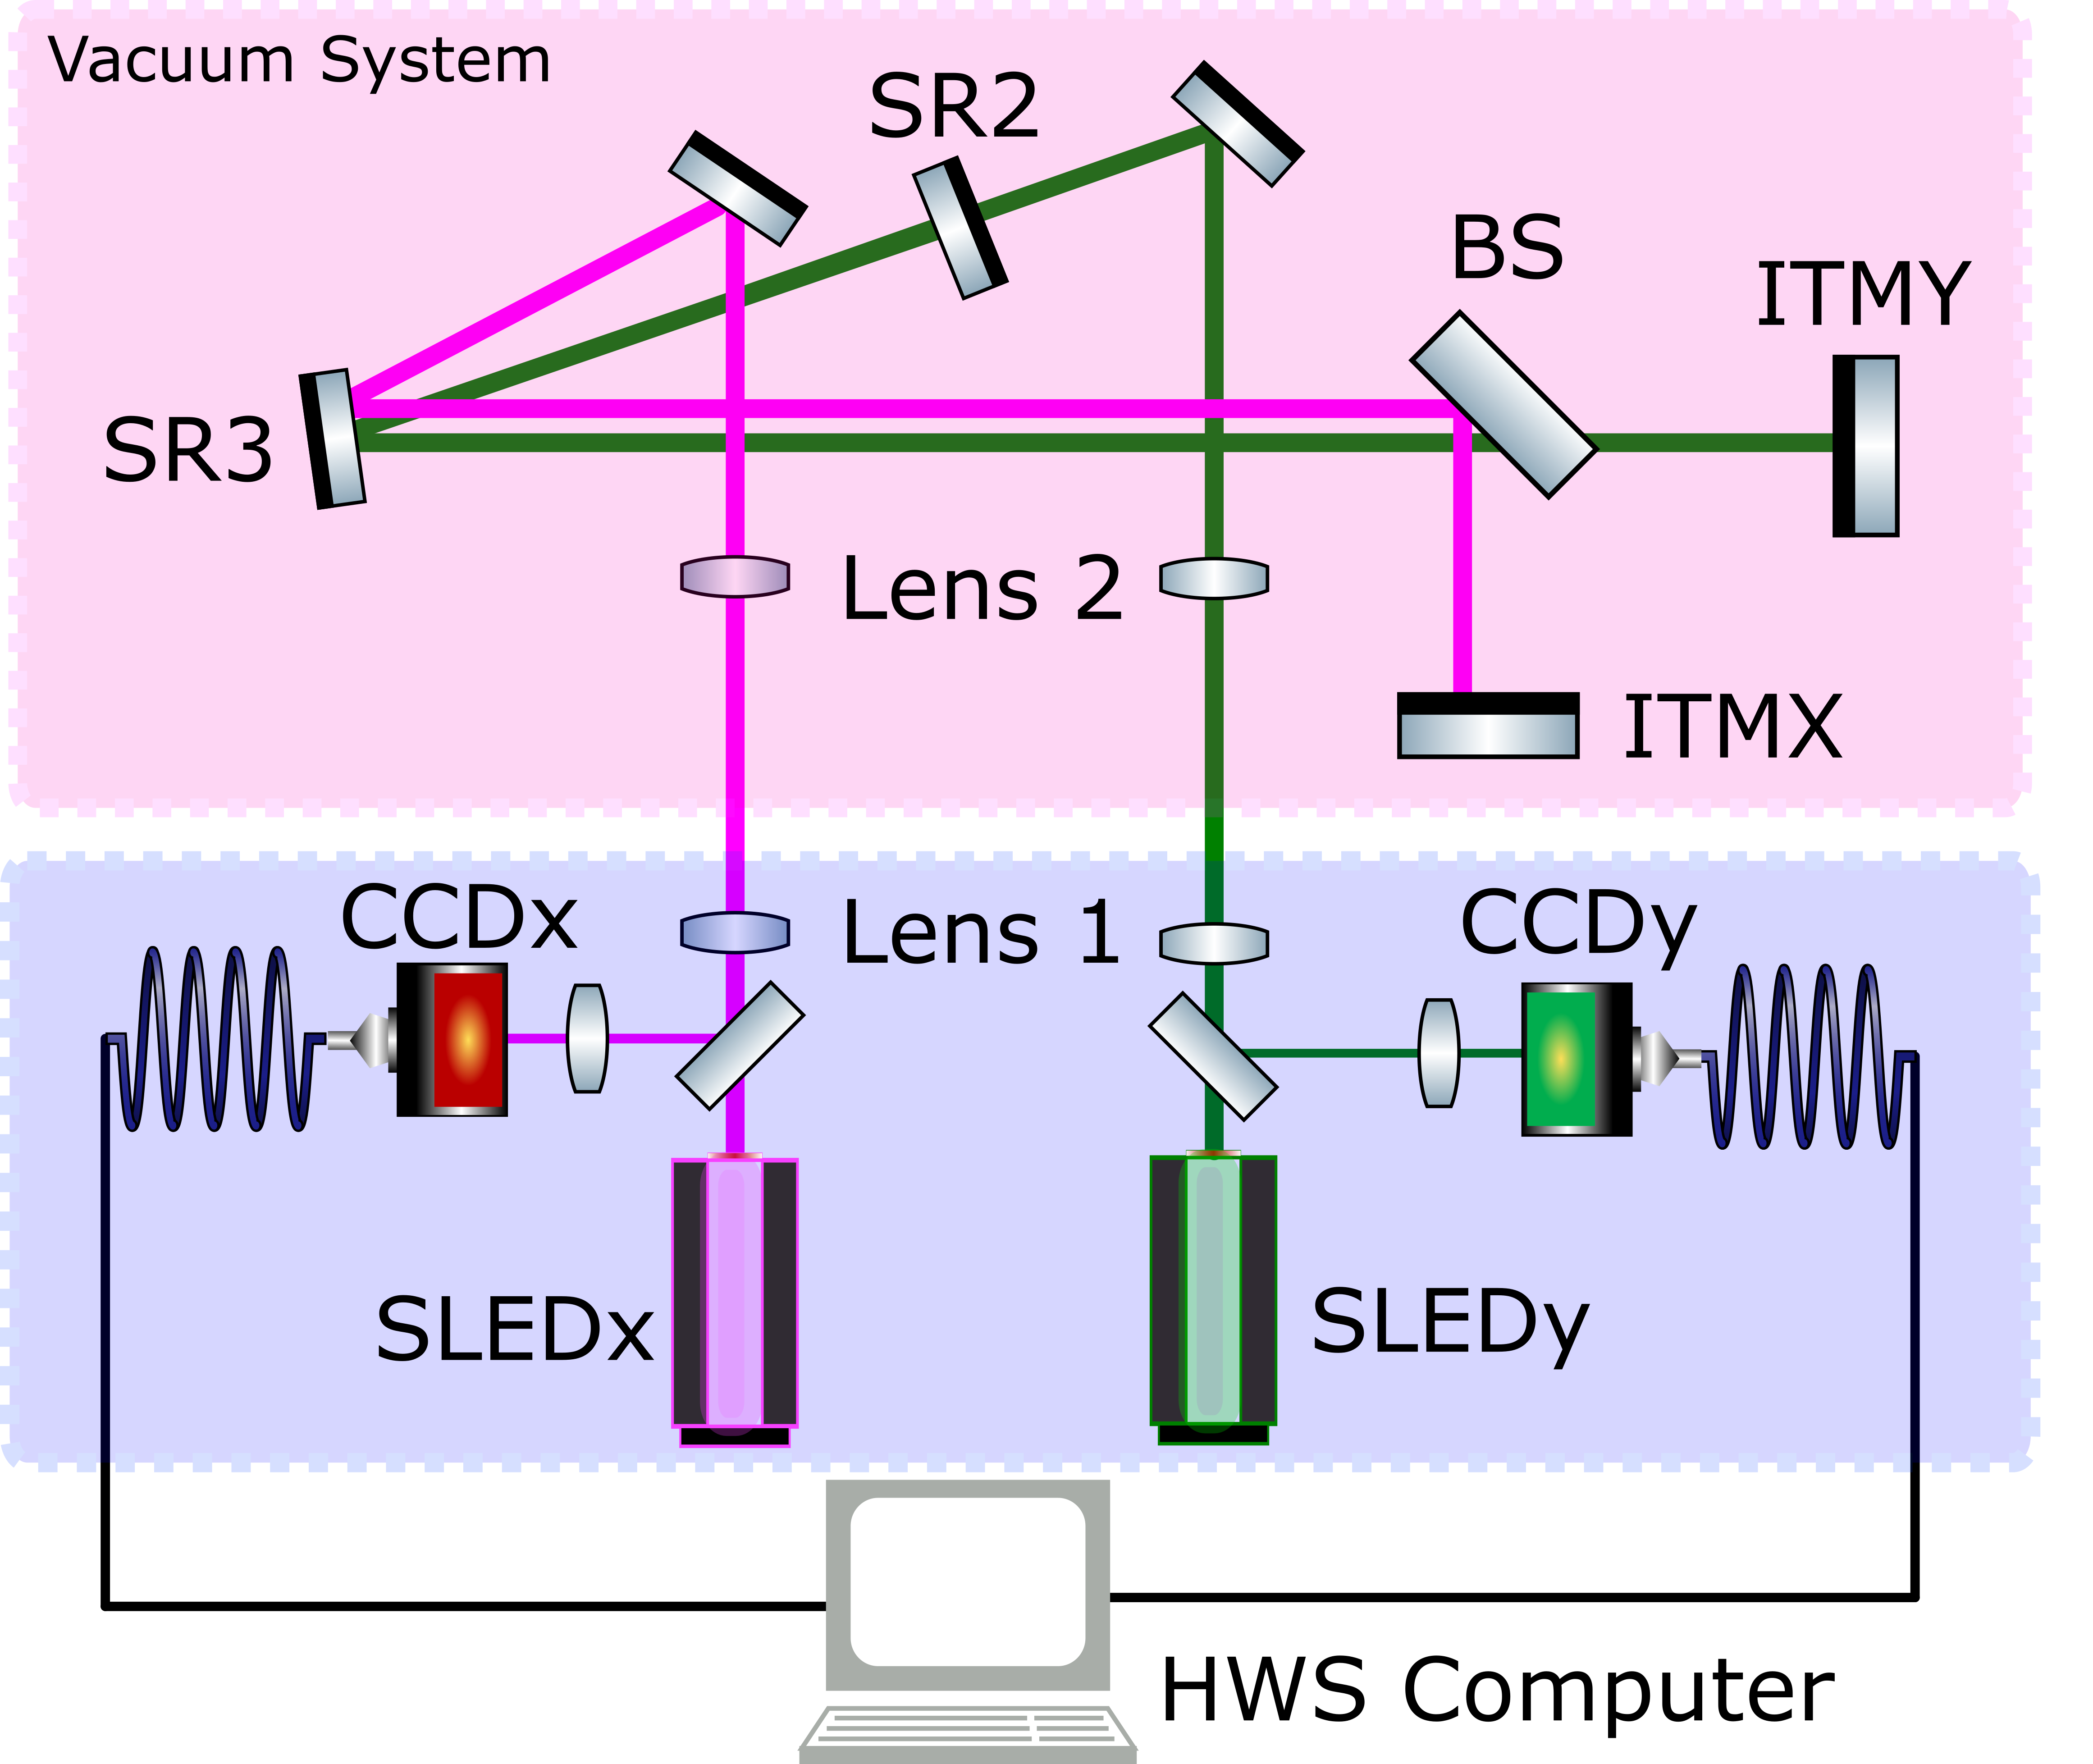
\includegraphics[width=0.6\textheight]{../Figures/HWS_OpticalLayout.png}
		\caption[ITM Hartmann sensors optical layout.] 
		{\textbf{ITM Hartmann sensors optical layout.} The path for injection is different for the two Hartmann sensors which use separate wavelengths to take advantage of the main beamsplitter AR/HR surface reflectivity. The ITMX (magenta) and ITMY (green) probe beam wavelengths are 800 nm and 833 nm, respectively, and have a 40 nm linewidth \cite{AWC_current}. The beams are sent into the vacuum system and retro-reflected off their respective optics back towards the pick-off mirrors before going into the CCDs with a Hartmann plate attached.  The cameras are then sent via fiber to a computer that runs the analysis pipeline on the images and exports the data to EPICS so the users can interface with the real time digital system in the control rooms.}
		\label{fig:HWS_optical}
	\end{figure}

	\begin{figure}[!]
	\centering
	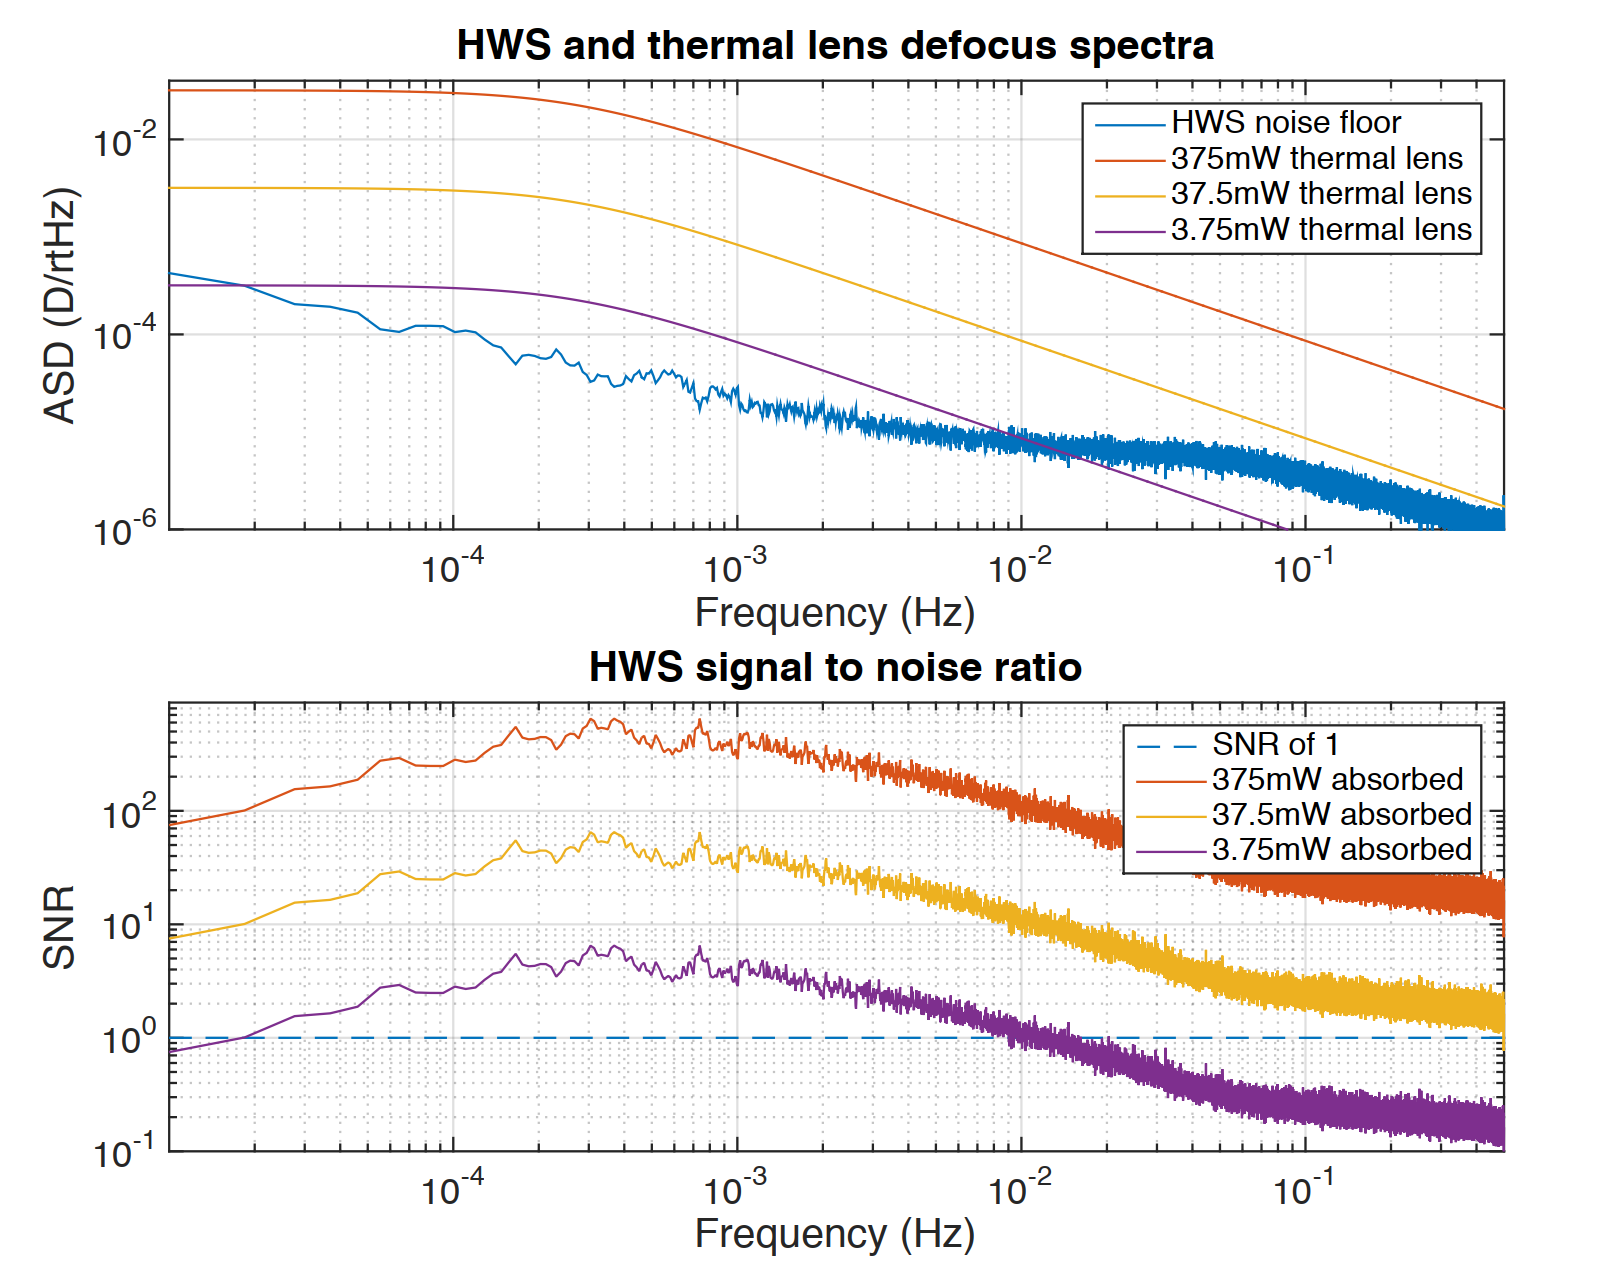
\includegraphics[width=0.7\textheight]{../Figures/HWS_Noise.PNG}
	\caption[Noise spectra for the HWS spherical lensing.] 
	{\textbf{Noise spectra for the HWS spherical lensing.} Taken from \cite{AWC_current}, this puts a lower bound on the Hartmann sensitivity to distortions for various time scales.}
	\label{fig:HWS_spectra}
	\end{figure}
	
	\subsubsection{Tuning the Hartmann Sensors}
	It was found that the CCDs (Dalsa pantera 1m60) had a number of hot pixels, which would create large spikes in their intensity counts and these produce large artifacts in the gradient plots that corrupted the spherical lens fitting (see Figure \ref{fig:HWS_Histogram}).  One of the requirements for the HWSs is a wavefront distortion resolution of 1.35 nm \cite{AWC_current} and a single hot pixel could register a few orders of magnitude higher.  A solution for this was implemented by using the dark images to locate the bad pixels by averaging the counts over a few minutes and finding all the pixels which have counts higher than a particular threshold, generally 1.5 times above the average ambient dark noise level (about 50 counts).  The dark frames would be read in by the Hartmann code, which uses the dark images as a reference to find the average of surrounding pixels and replace the problematic pixel.  This digital procedure greatly reduced the impact of hot pixels in the Hartmann sensor data.
	
	\begin{figure}[!]
		\centering
		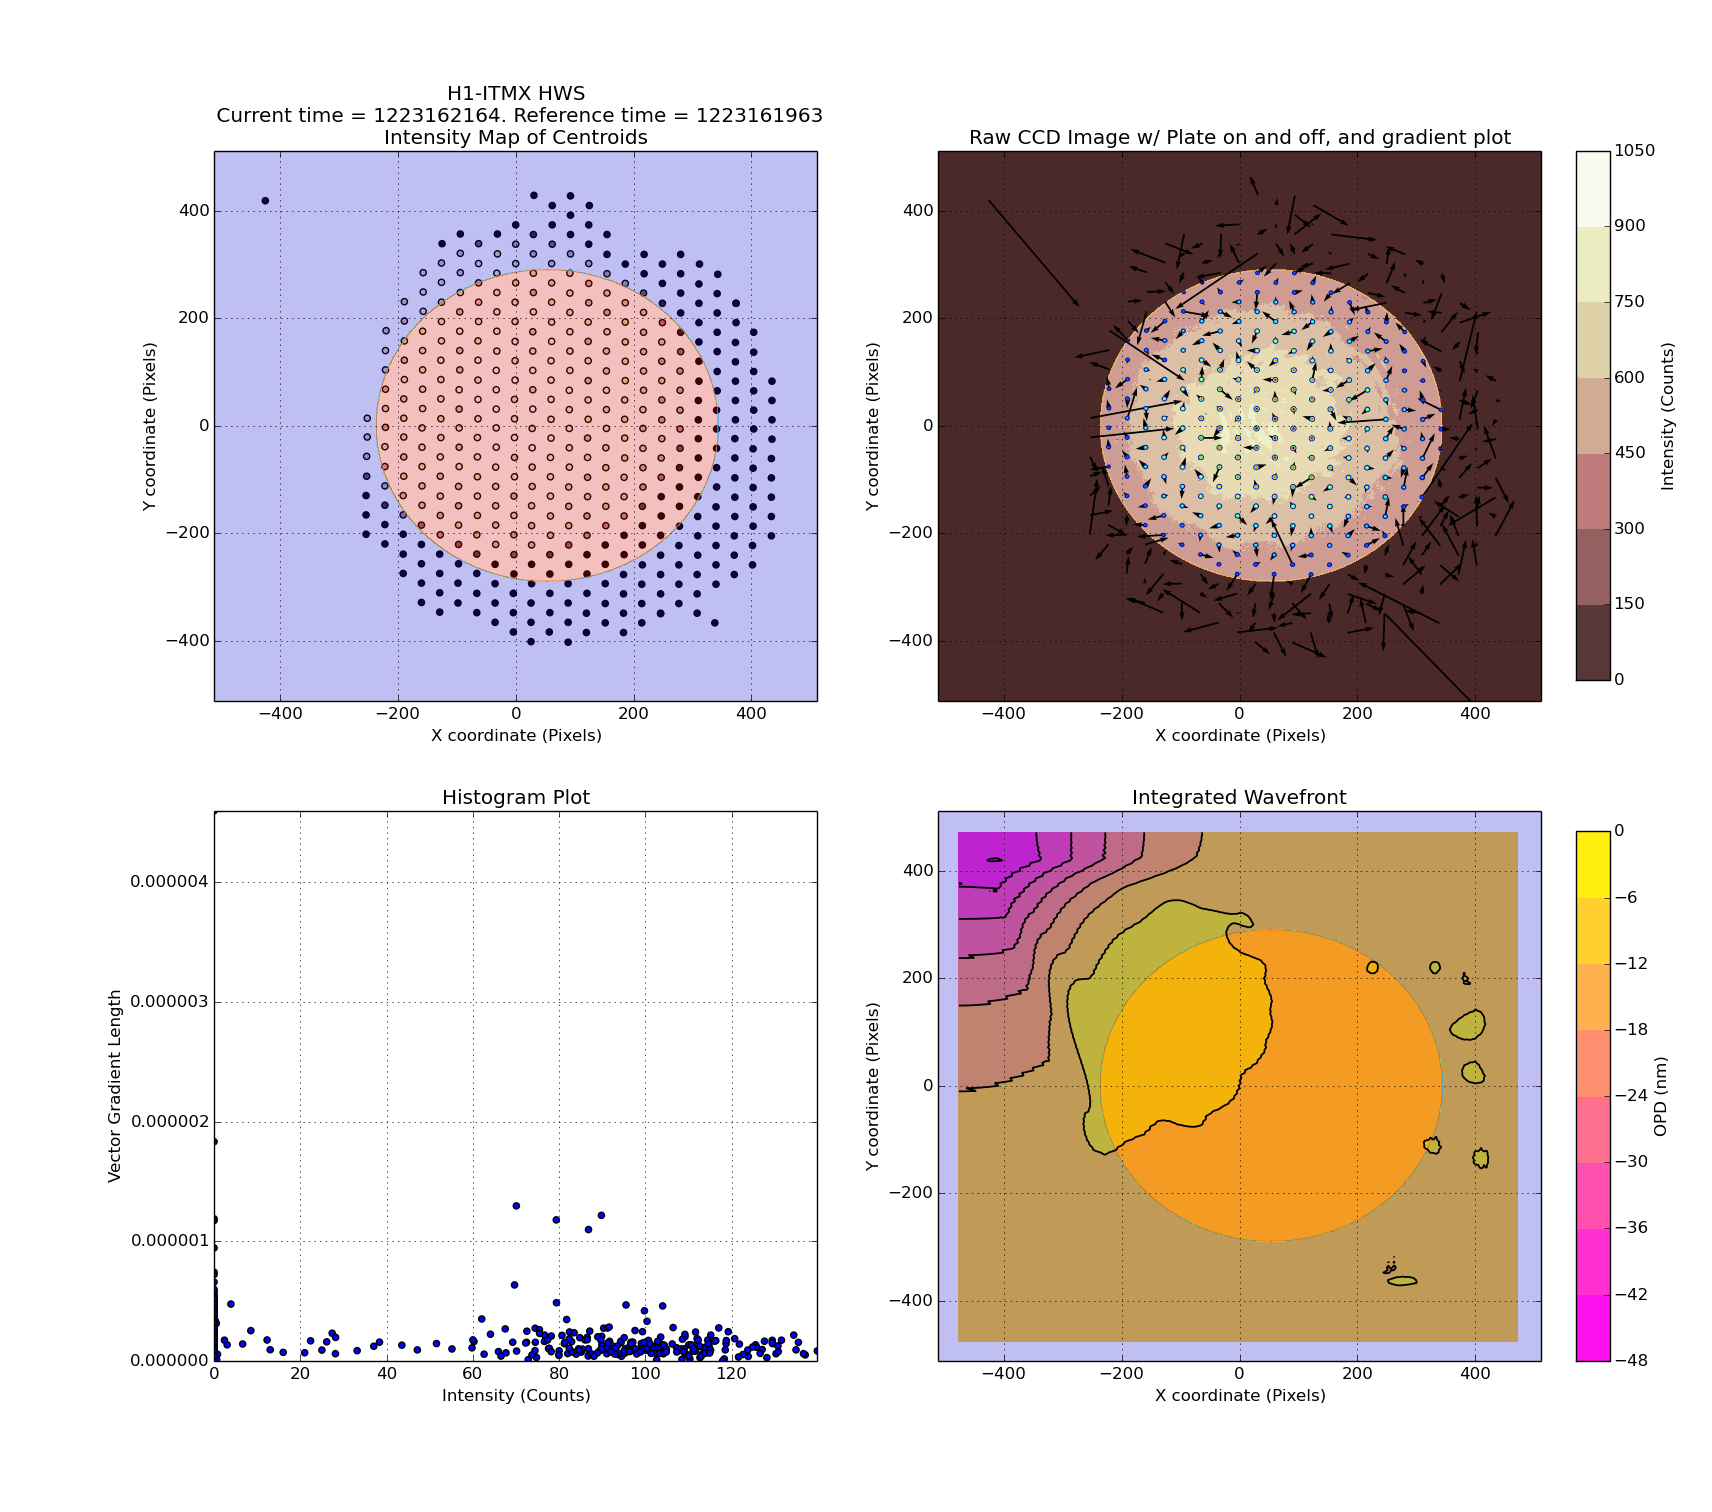
\includegraphics[width=0.7\textheight]{../Figures/20181011_ITMX_HWS_histogram_Masked.png}
		\caption[ITMX Hartmann Sensor output.] 
		{\textbf{ITMX Hartmann Sensor output.} Between the reference and current times for this measurement, no heating was applied to the test masses so the expectation is a relatively flat and smooth wavefront. This is mostly true except for a large, anomalous arrow at pixel coordinate [X,Y] = [-410, 405] of the gradient plots (upper right) which leads to a false wavefront distortion in the same area for the contour plot (lower right).  The sharp iris in the middle represents a digital mask that is can be turned on to reduce the effects of fringing.  A histogram in the bottom left plot shows the intensity distribution for each of the gradients; if the HWS beams are co-aligned well with the interferometer beam, then most of the information about thermal lensing occurs near the center of the intensity distribution.}
		\label{fig:HWS_Histogram}
	\end{figure}
	Another source of systematic error was from beam clipping along the in-vacuum beam path on the ITMX HWS, see Figure \ref{fig:ITMX_clipping}. This creates diffraction fringes which are extremely sensitive to misalignment; one fix that was applied to reduce this noise was to digitally mask the fringes so they do not confuse the fitting algorithms.  Hand tuning must be done so that the mask is wide enough and centered around the interferometer lensing but not so large that the Hartmann fitting is corrupted by the fringes. Two in-air periscope mirrors with pico-motors were used for alignment, but beam clipping could not be fully removed.  This artifact was also found at LLO so it suggests a design flaw in the initial alignment scheme.  A possible fix could be implemented by replacing an in-vacuum steering mirror with a pico-motor that could be aligned remotely.

	
	\begin{figure}[t!]
		\centering
		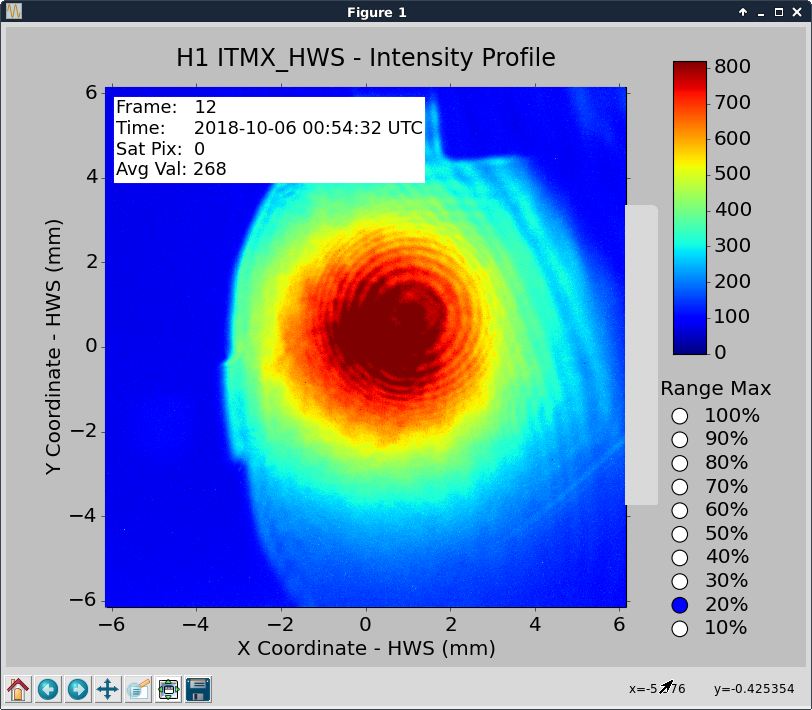
\includegraphics[width=0.4\textheight]{../Figures/ITMX_HWS_clipping.png}
		\caption[Clipping on ITMX Hartmann Sensor.] 
		{\textbf{Clipping on ITMX Hartmann Sensor.}  A source of systematic error found at both sites when trying to simultaneously align ITMX and ITMY Hartmann Sensors.  The CCD spot positions are very sensitive to the SR3 alignment so control loops and initial alignment are not recommended for this particular optic.  An in-vacuum pico-motor may help alleviate the clipping.
		}
		\label{fig:ITMX_clipping}
	\end{figure}
	
	When increasing the input power into the interferometer, there were large spikes associated with the spherical power estimation on the ITMX corresponding to time scales of less than a second which is not likely due to lensing from uniform absorption.  This was eventually tracked down to a leakage beam caused by stray light from the interferometer.  At times, the leakage beam was 40\% the intensity of the main Hartmann beam which severely distorted the fitting algorithms. ITMY HWS did not see this effect because SR2 is such a good high reflector and attenuated any 1064 nm contributions down to the ppm level.
	
	\begin{figure}[t!]
		\centering
		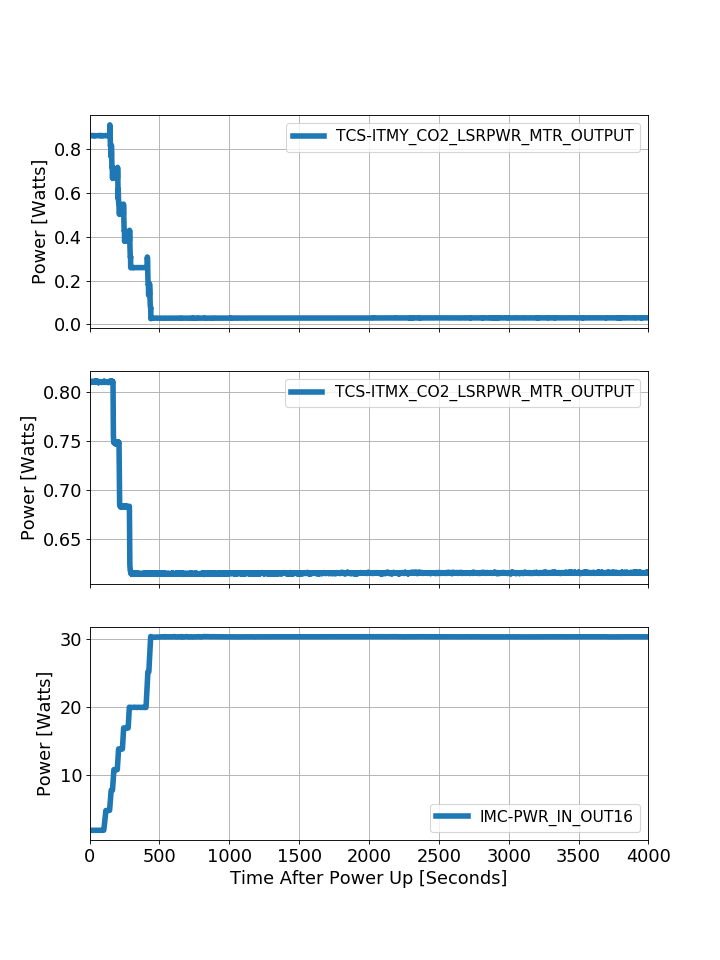
\includegraphics[width=0.45\textwidth]{../Figures/1231726400TCS_and_PSL_powerup.png}
		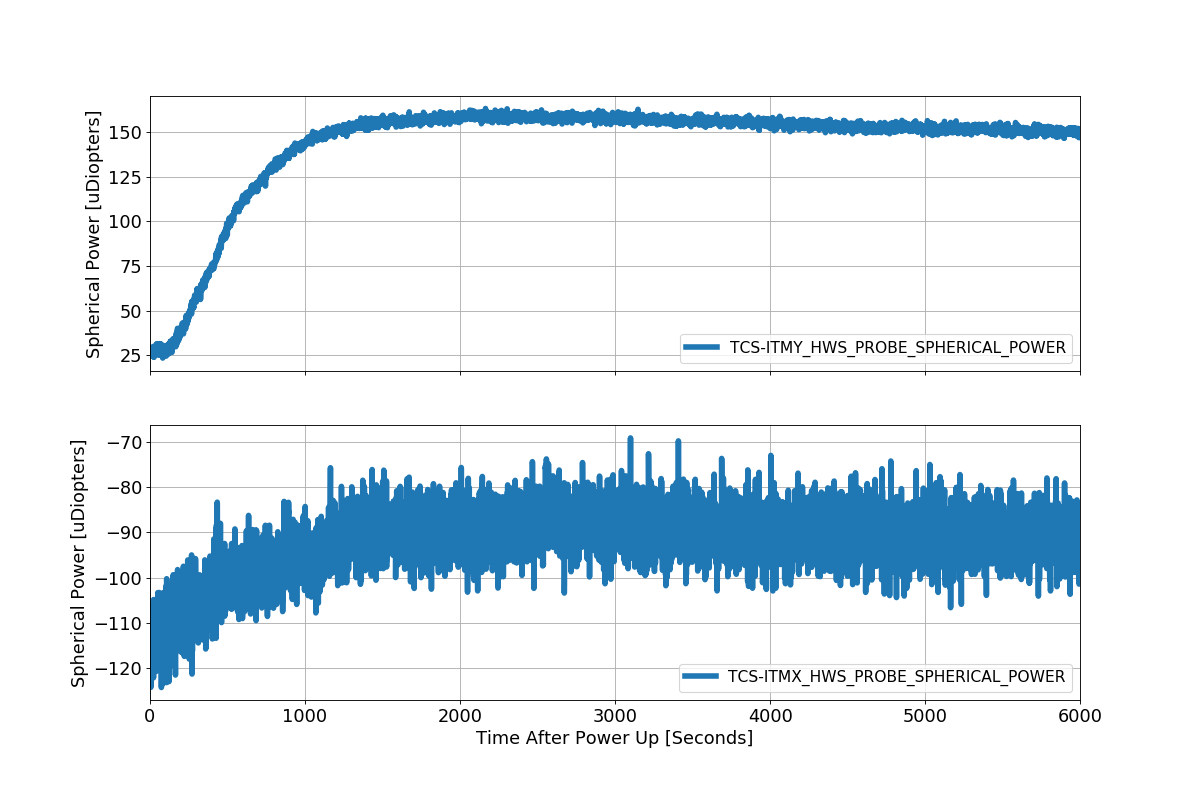
\includegraphics[width=0.45\textwidth]{../Figures/1231726400HWS_powerup.png}
		\caption[A time series of the interferometer power increase sequence.] 
		{\textbf{A time series of the interferometer power increase sequence.} 
			During this time, the interferometer is using DC-readout and locked at 2 watts of PSL input power with all of the angular control loops closed with high-bandwidth, in this configuration, the power recycling gain is approximately 45.  The left figure shows the increase of PSL input power (bottom) and the CO$_2$ lasers (top two) stepping down in power where levels of compensation were experimentally determined such that the angular control loops were stable and sideband build ups remained as high as possible.  The right plot shows the Hartmann sensor spherical power as a function of time with the starting point scaled to zero micro-diopters for ITMX and ITMY.  Although the point absorbers do not exhibit the same spatial structure as uniform heating so it is difficult to derive absolute absorption for ITMY, the spherical fitting gives some information about the relative scale of heating absorption between the two optics.}
		\label{fig:pwr_up_time}
	\end{figure}
	
	\begin{figure}[t!]
		\centering
		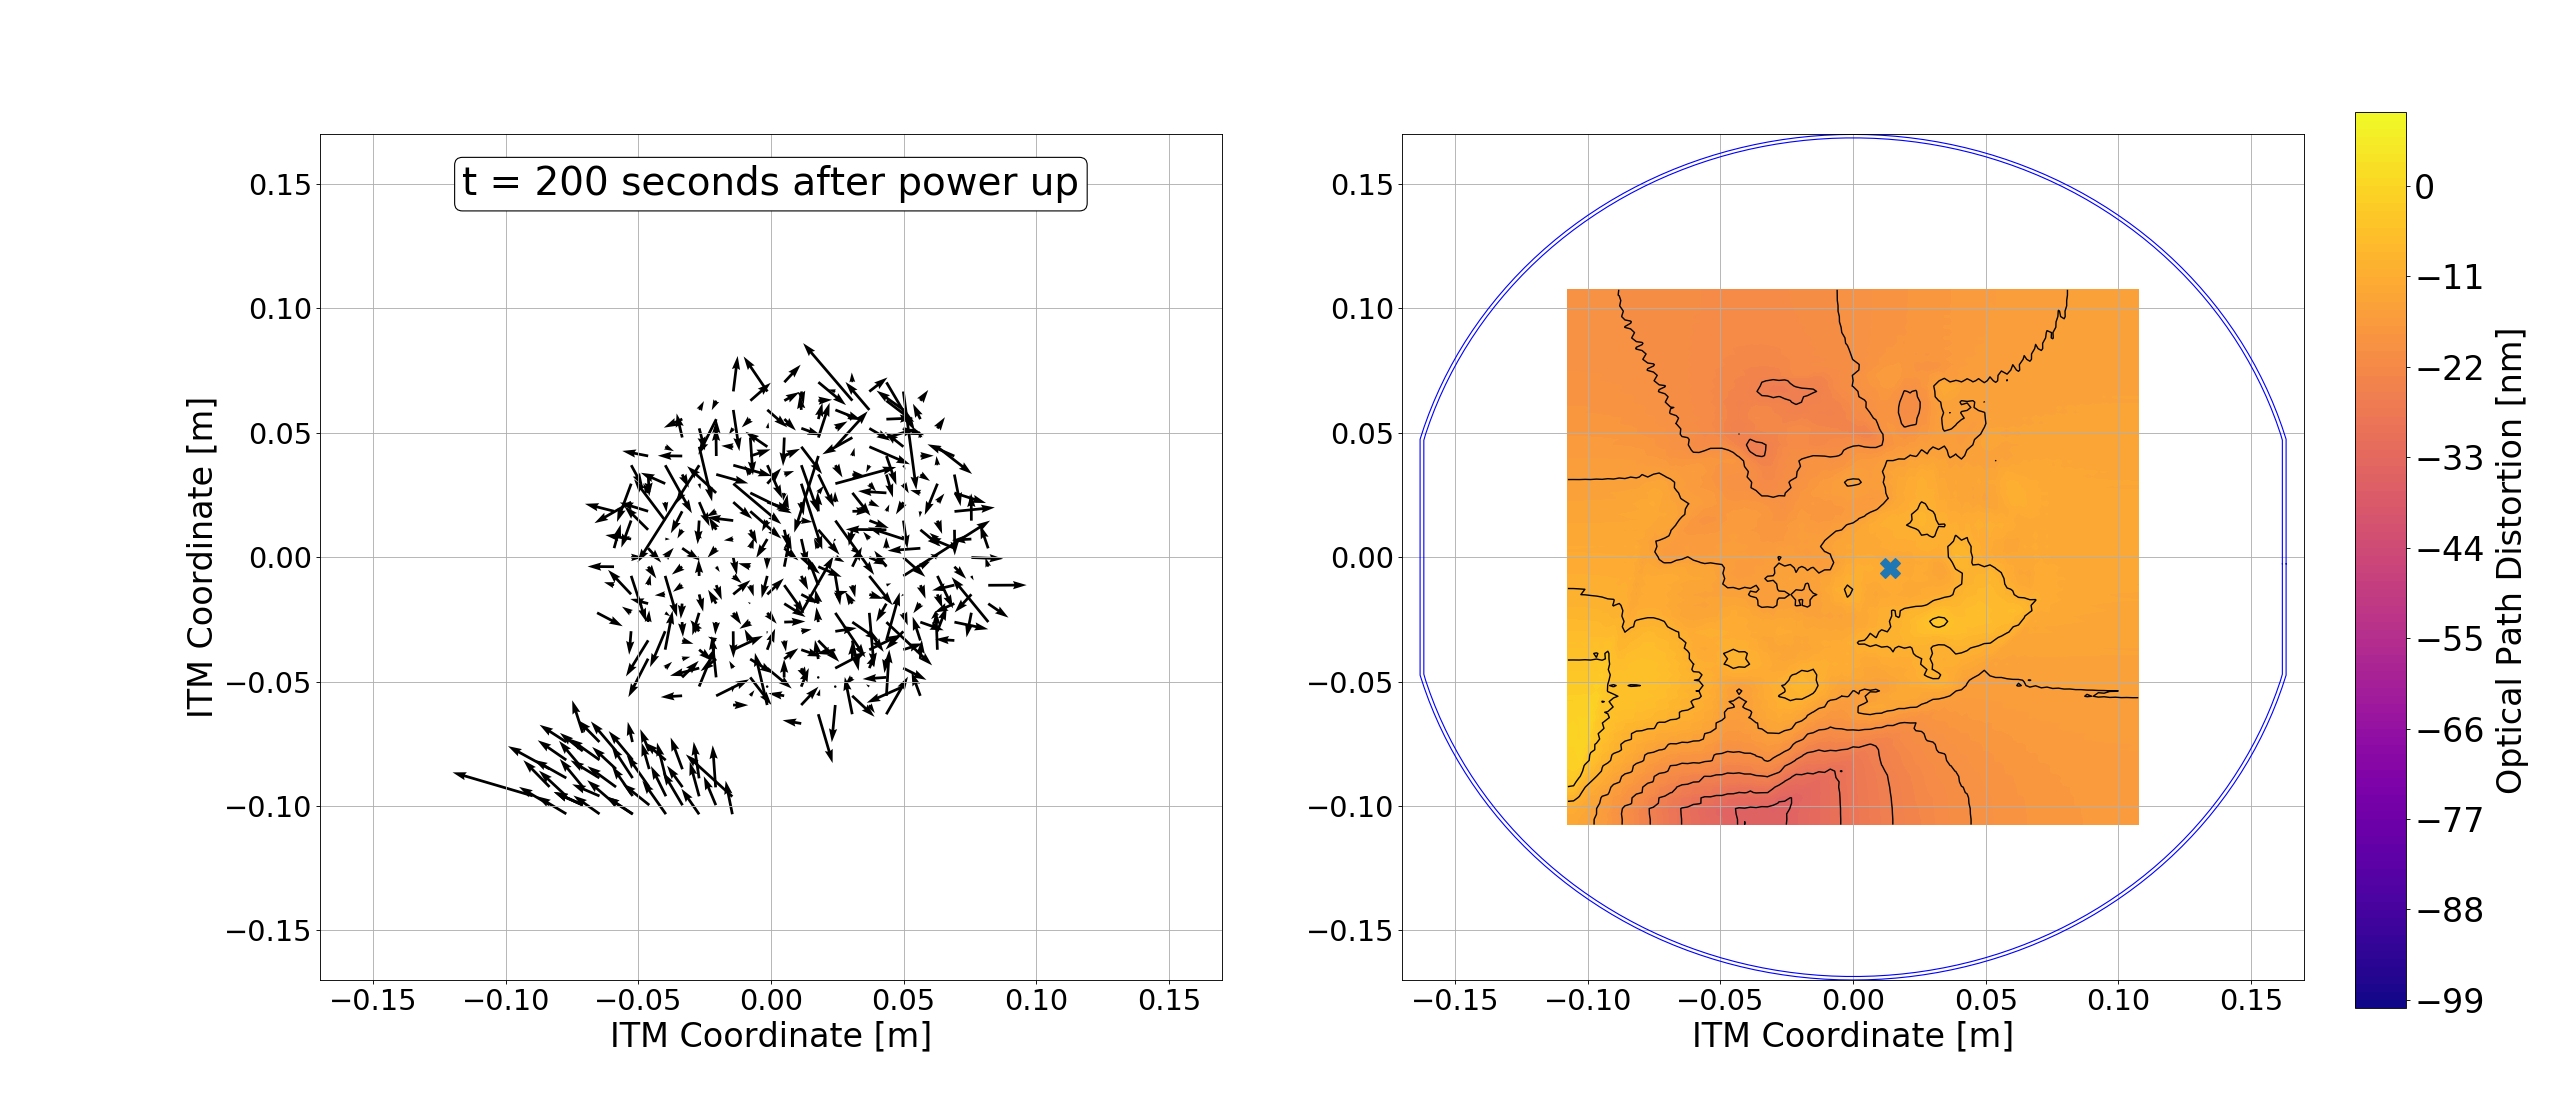
\includegraphics[width=0.55\textheight]{../Figures/1231726400_200dur_30W_ITMx.png}\quad
		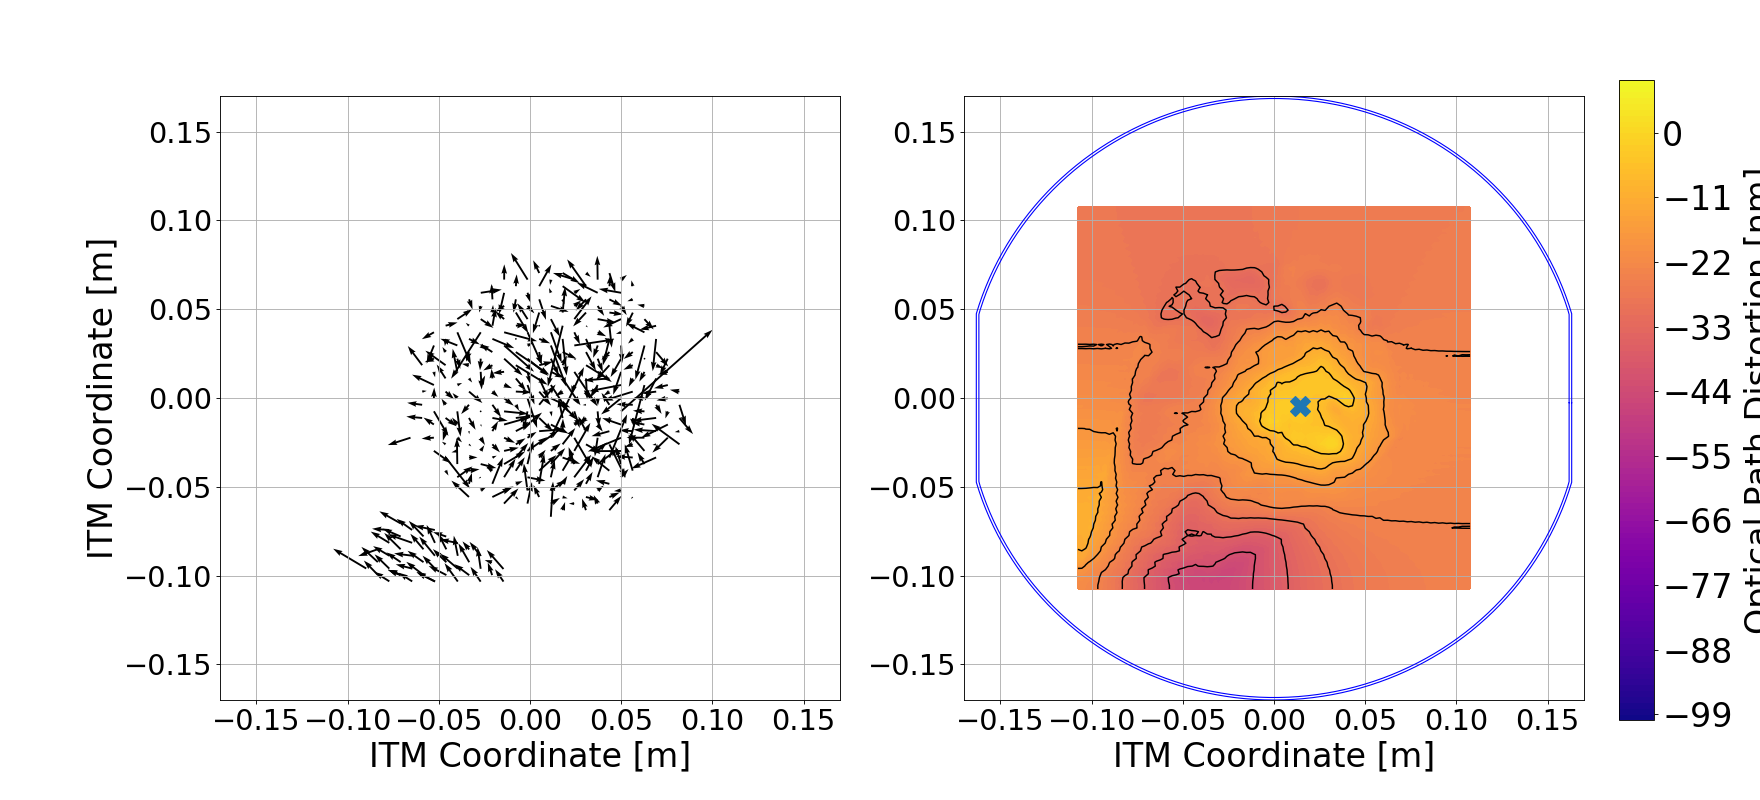
\includegraphics[width=0.55\textheight]{../Figures/1231726400_500dur_30W_ITMx.png}\quad
		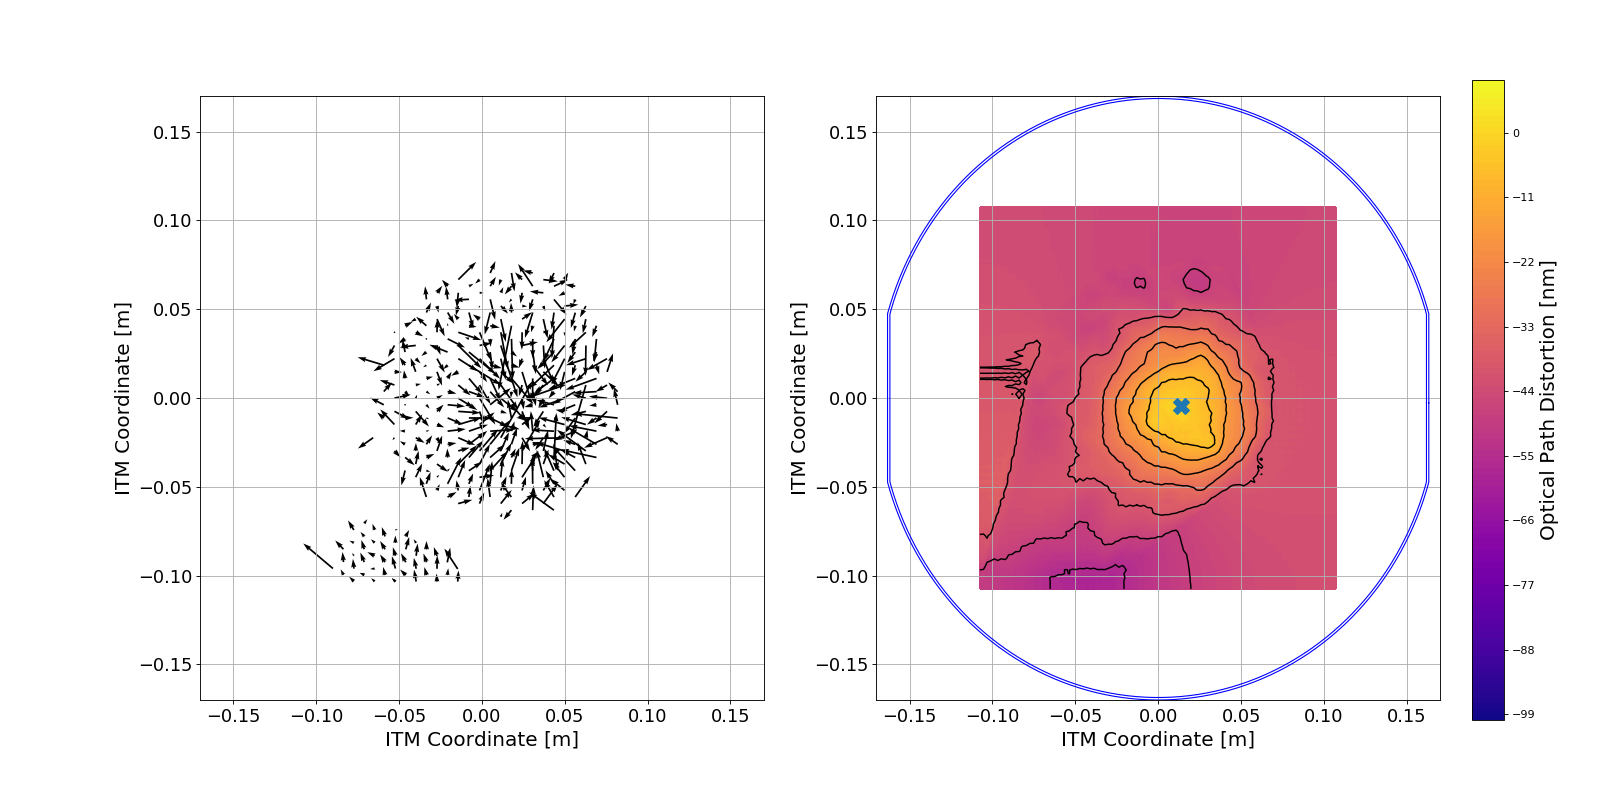
\includegraphics[width=0.55\textheight]{../Figures/1231726400_1000dur_30W_ITMx.png}\quad
		\caption[ITMX gradient plots (left) and wavefront maps (right) during a power up to 30 Watts of input power.]  
		{\textbf{ITMX gradient plots (left) and wavefront maps (right) during a power up to 30 Watts of input power.}
			It is important to note that there is a back-reflected stray beam from the super-luminous LED that is incident in the bottom left portion of the camera which is digitally cropped out during the real-time analysis. As previously noted, this particular Hartmann sensors suffers from beam clipping on the right side of the image which adds to the systematic noise.  A blue cross denotes the origin which is fitted with the Zernike polynomials to derive a spherical power.  The arrow lengths in the gradient plots are normalized to each individual plot and are meant to guide the eye in discerning the directionality and pattern of lensing.}
		\label{fig:ITMX_HWS_plot}
	\end{figure}
	
	\begin{figure}[t!]
		\centering
		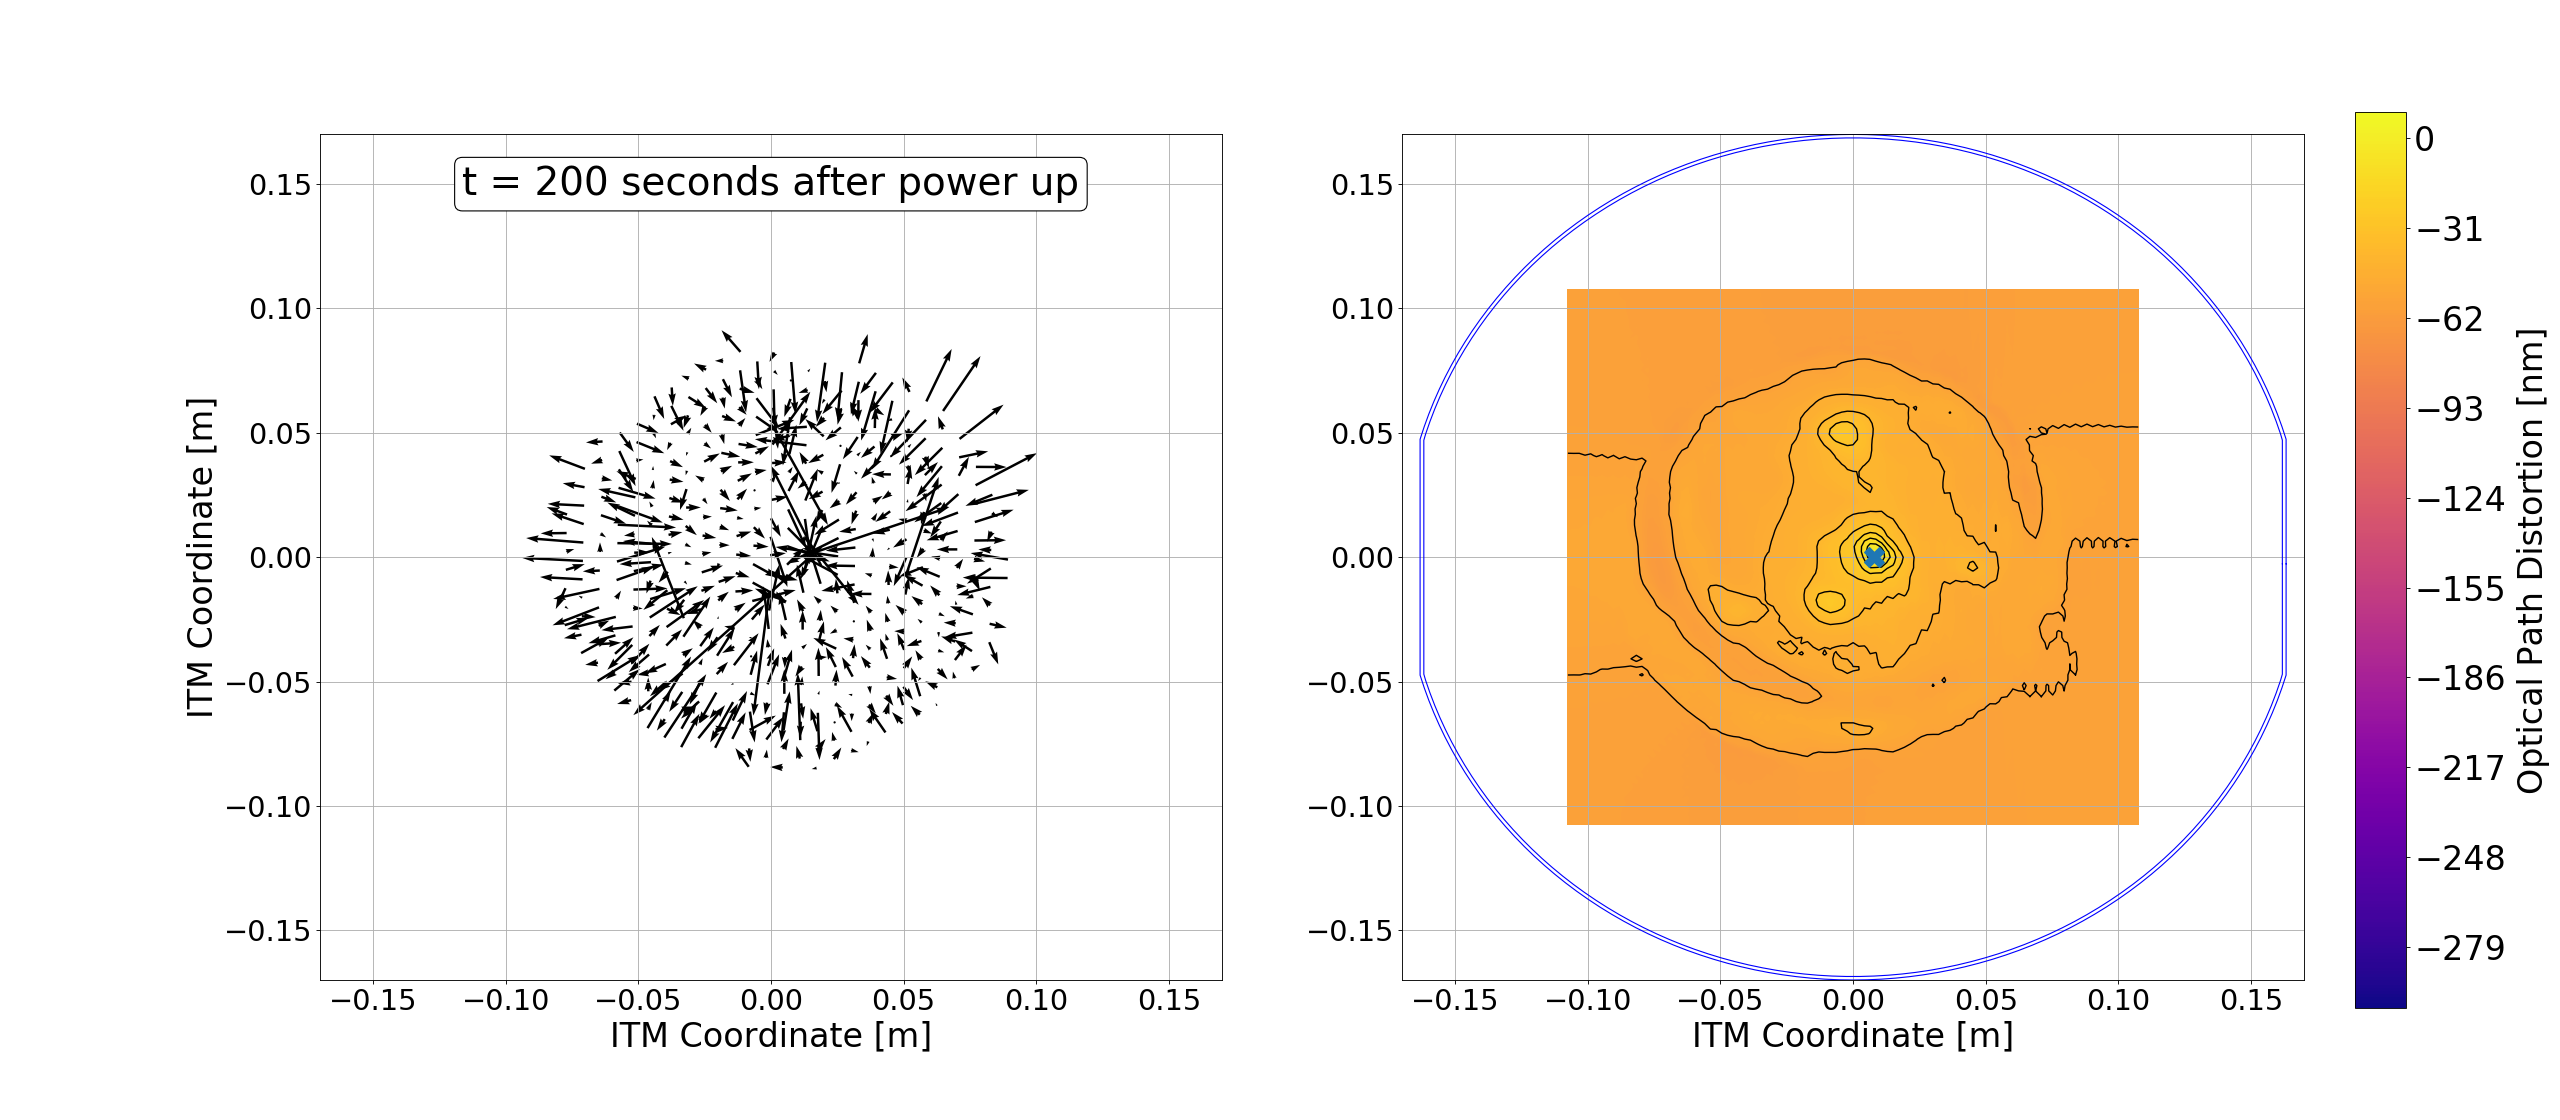
\includegraphics[width=0.55\textheight]{../Figures/1231726400_200dur_30W_ITMy.png}\quad
		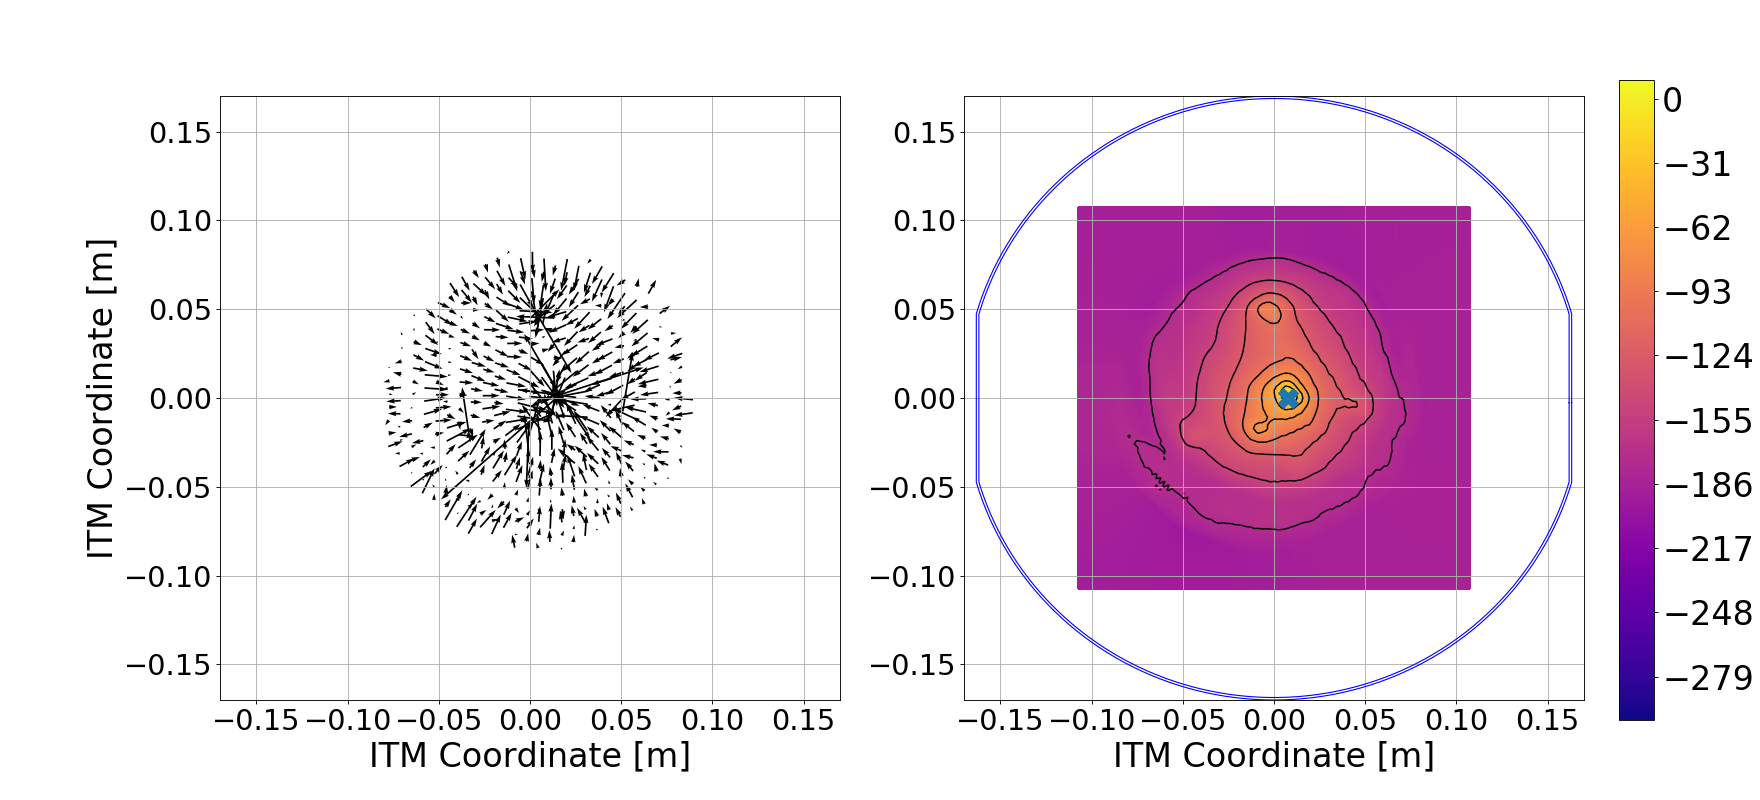
\includegraphics[width=0.55\textheight]{../Figures/1231726400_500dur_30W_ITMy.png}\quad
		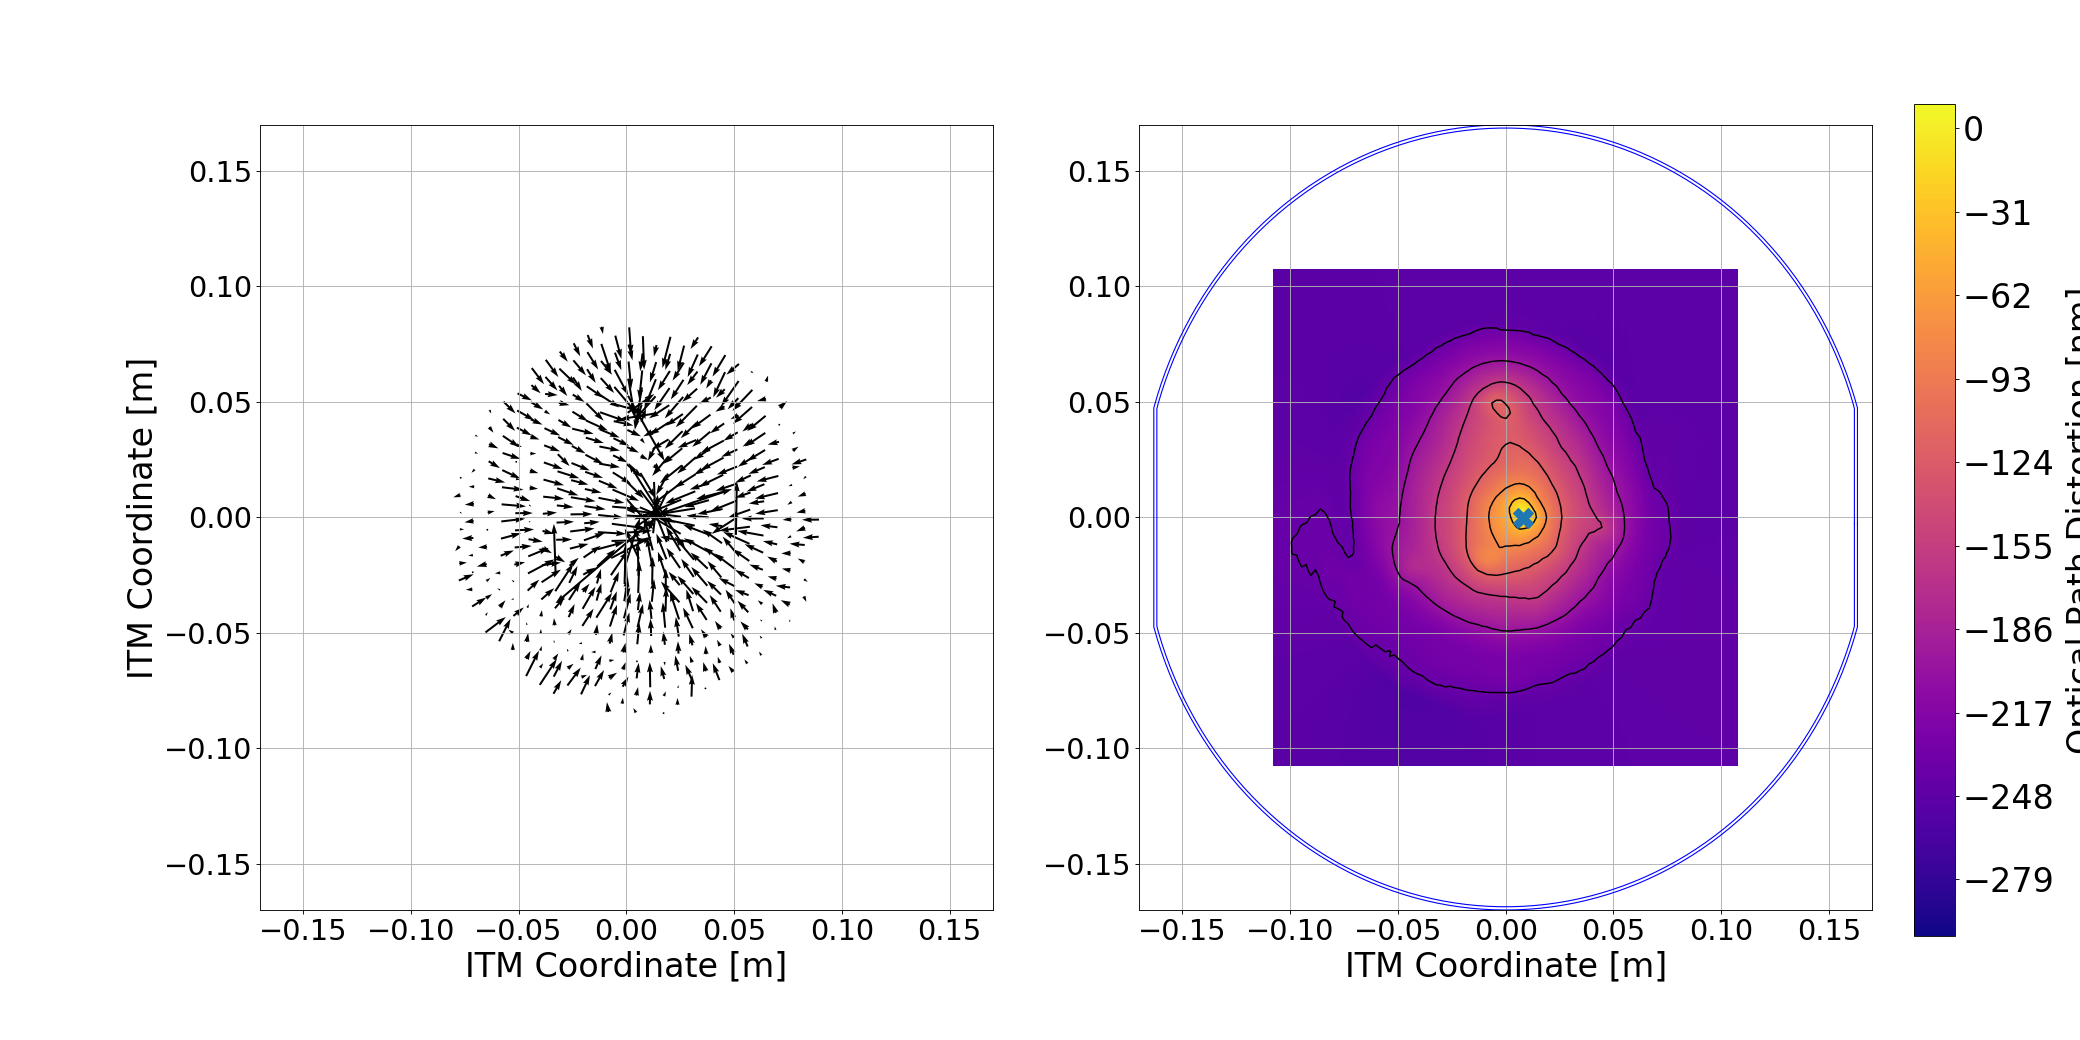
\includegraphics[width=0.55\textheight]{../Figures/1231726400_1000dur_30W_ITMy.png}\quad
		\caption[ITMY gradient plots (left) and wavefront maps (right) during a power up to 30 Watts of input power.]  
		{\textbf{ITMY gradient plots (left) and wavefront maps (right) during a power up to 30 Watts of input power.}
			Compared to the ITMX phase map in Figure \ref{fig:ITMX_HWS_plot}, ITMY has a much larger overall heating pattern and higher spatial frequencies in the contours which was the first clue that revealed multiple (possibly 4) point absorber on the test mass.  There is also a halo of gradients on the outer rim of the plots which is most prominent on the lower left corner.  This is due reducing the CO$_2$ laser power in an attempt to compensate the lensing effects as the interferometer beam heats up the test mass.  The overall scale of self-heating with the higher spatial frequencies of the point absorbers makes it very difficult to compensate with using the CO$_2$ lasers as designed by Advanced LIGO. }
		\label{fig:ITMY_HWS_plot}
	\end{figure}

	\subsubsection{Measuring Uniform Absorption}
	After the arm power drops suddenly, the lensing decays exponentially at a rate that depends on the amount of absorption on the high reflective surfaces of the arm cavity.  Using the HWS, it is possible to fit the decay rate to a finite element model of a cylindrical mass in order to solve for a single uniform absorption estimate.  It is extremely important to have reliable measurements to aid in pre-determining the amount compensation necessary to prepare the test masses for lock acquisition.  
	
	Figure \ref{fig:hws_abs} shows the measured spherical power from interferometer heating for ITMX/ITMY and comparing the two optics shows that the spherical power difference for ITMY is almost a factor of 2 larger than ITMX. Applying an Markov Chain Monte-Carlo method allows some statistical uncertainty estimates for the exponential fitting to the data shown in Figure \ref{fig:mcmc_hws_abs}, where the priors are assumed to be random Gaussian noise and the initial guesses are scaled roughly with a least squares fitting algorithm. One of the main differences between the O2 and O3 observing runs was the replacement of ITMX, ETMX, and ETMY test masses.  With a fully running Hartmann Sensor system in place which monitors the wavefront curvature across the optic, long-term trends over the observation runs will be able to determine how absorption changes as a function of time and whether test masses have an innate lifetime.  This will be particularly important if the next generation of detectors use much higher power levels in order to achieve better high frequency sensitivity \cite{DanBrown_prvt}.  Using this method, the current absorption estimates for the H1 input test masses are as follows:
	\begin{equation}
	\begin{aligned}
	A_{\text{ITMX}} &= 328 \pm 84 \; \text{ppb}\\
	A_{\text{ITMY}} &= 688 \pm 85 \; \text{ppb}
	\end{aligned}
	\end{equation}
	\begin{figure}[!]
		\centering
		\begin{subfigure}[a]{0.8\textwidth}
			\centering
			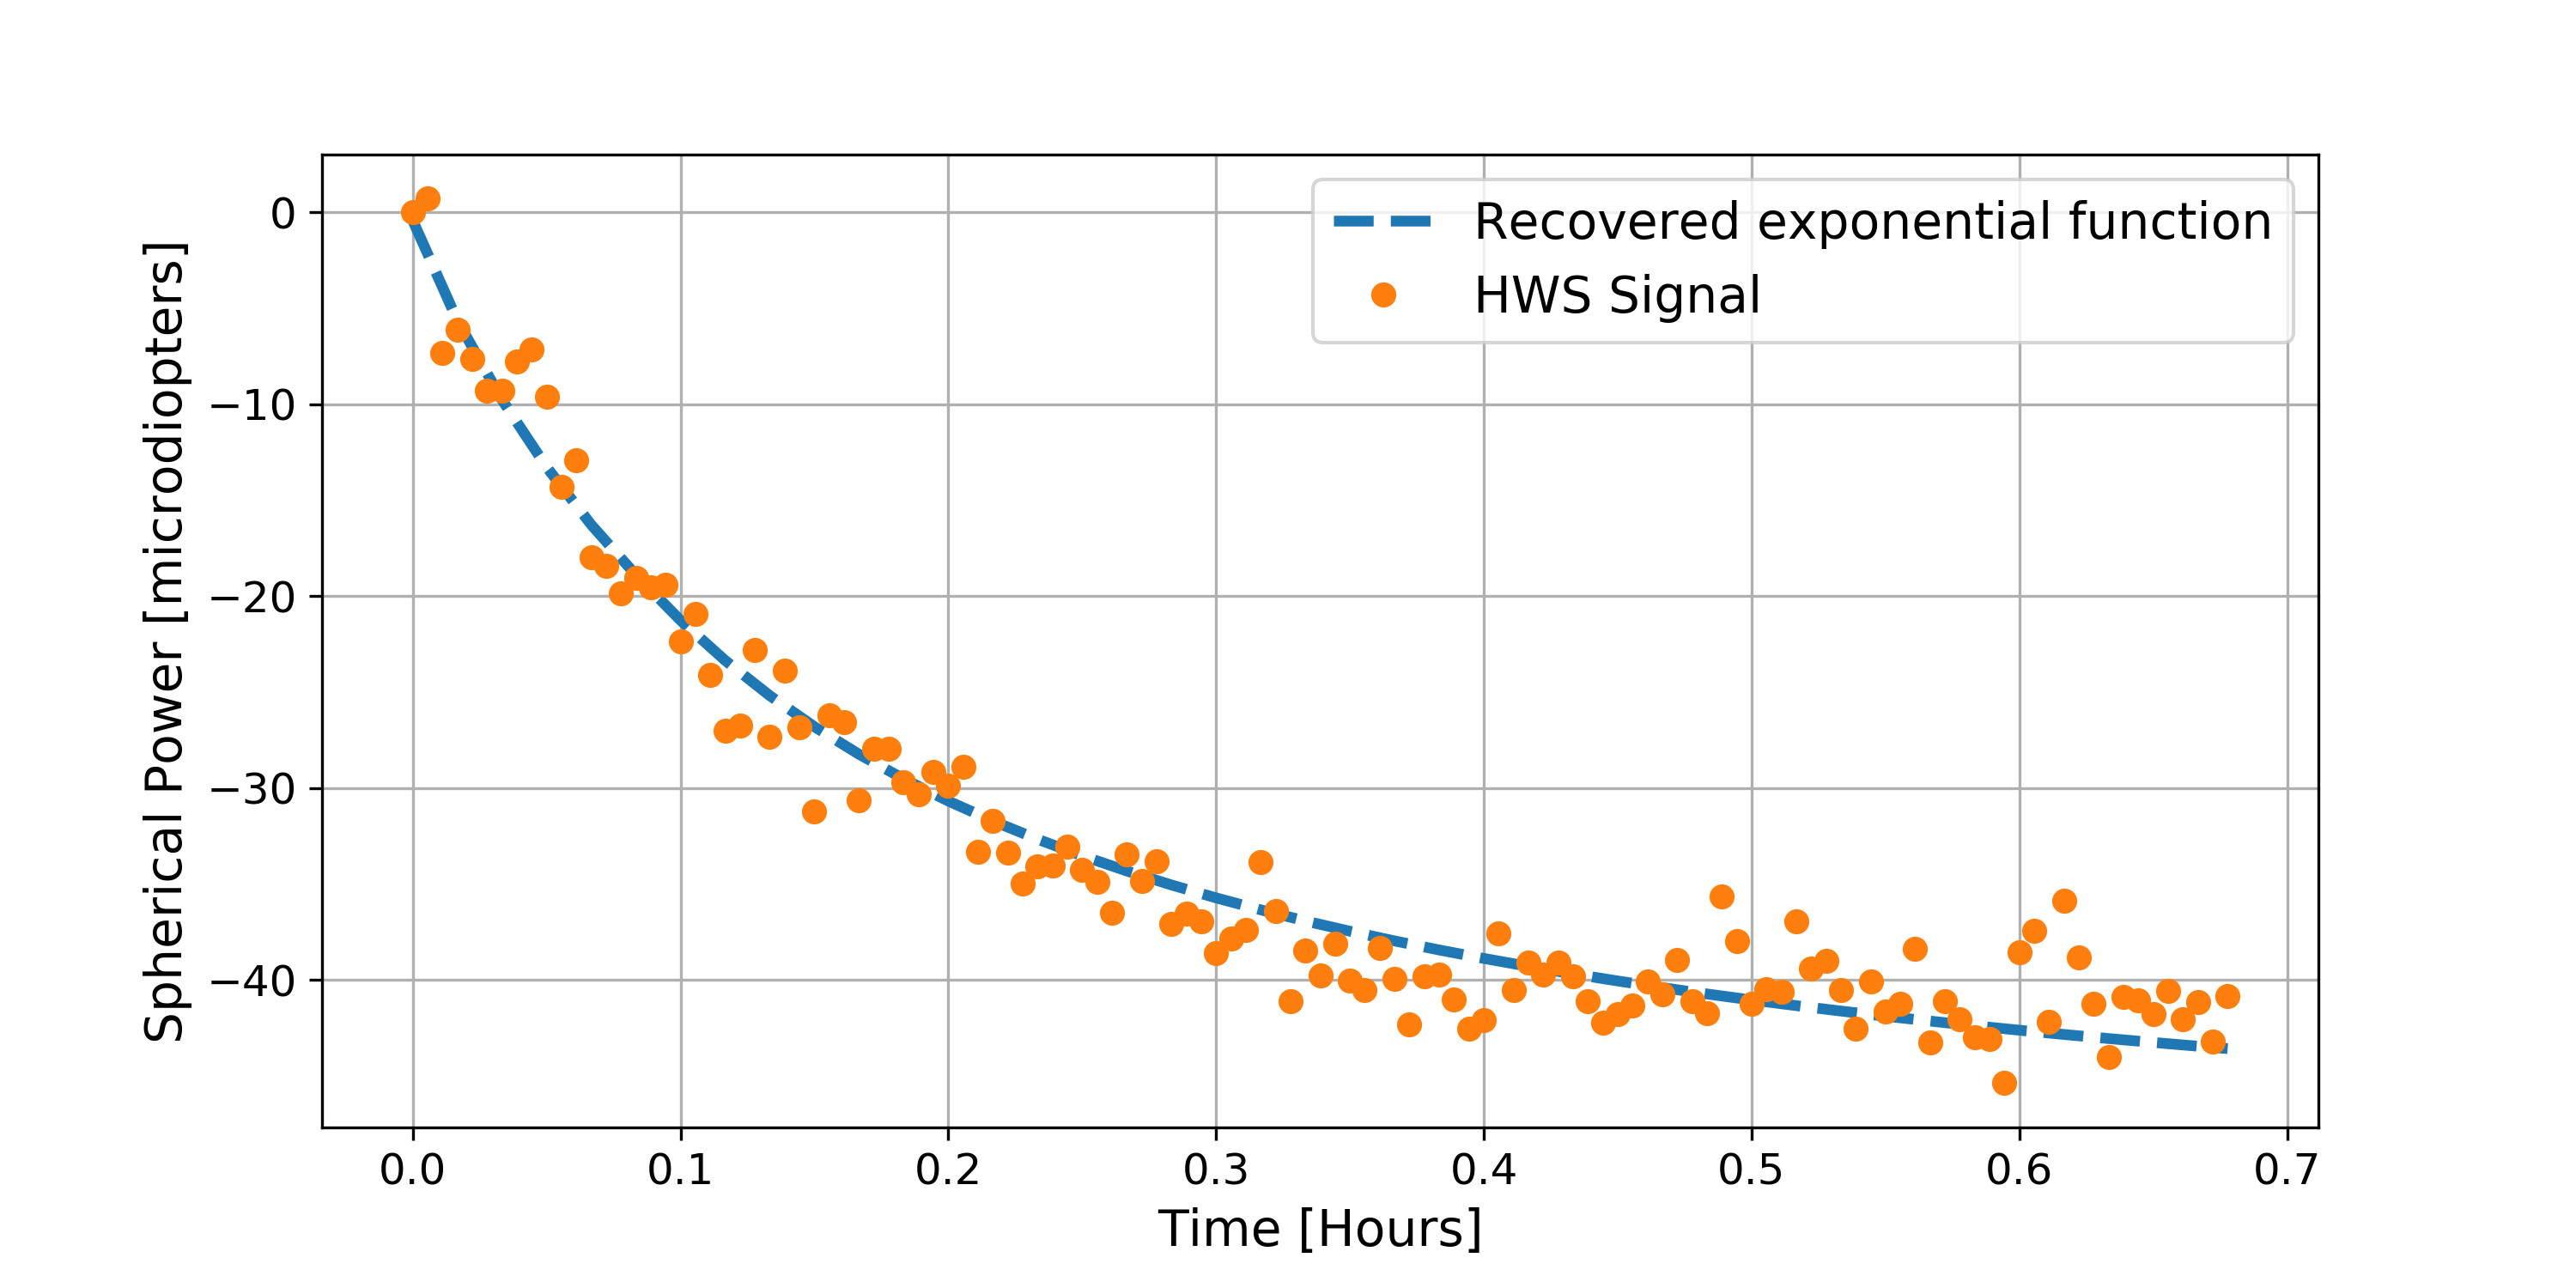
\includegraphics[width=\textwidth]{../Figures/MCMC_ITMX_ABS_FIT.png}
			\caption{ITMX absorption}
			\label{fig:itmx_abs}
		\end{subfigure}
		\hfill
		\begin{subfigure}[b]{0.8\textwidth}
			\centering
			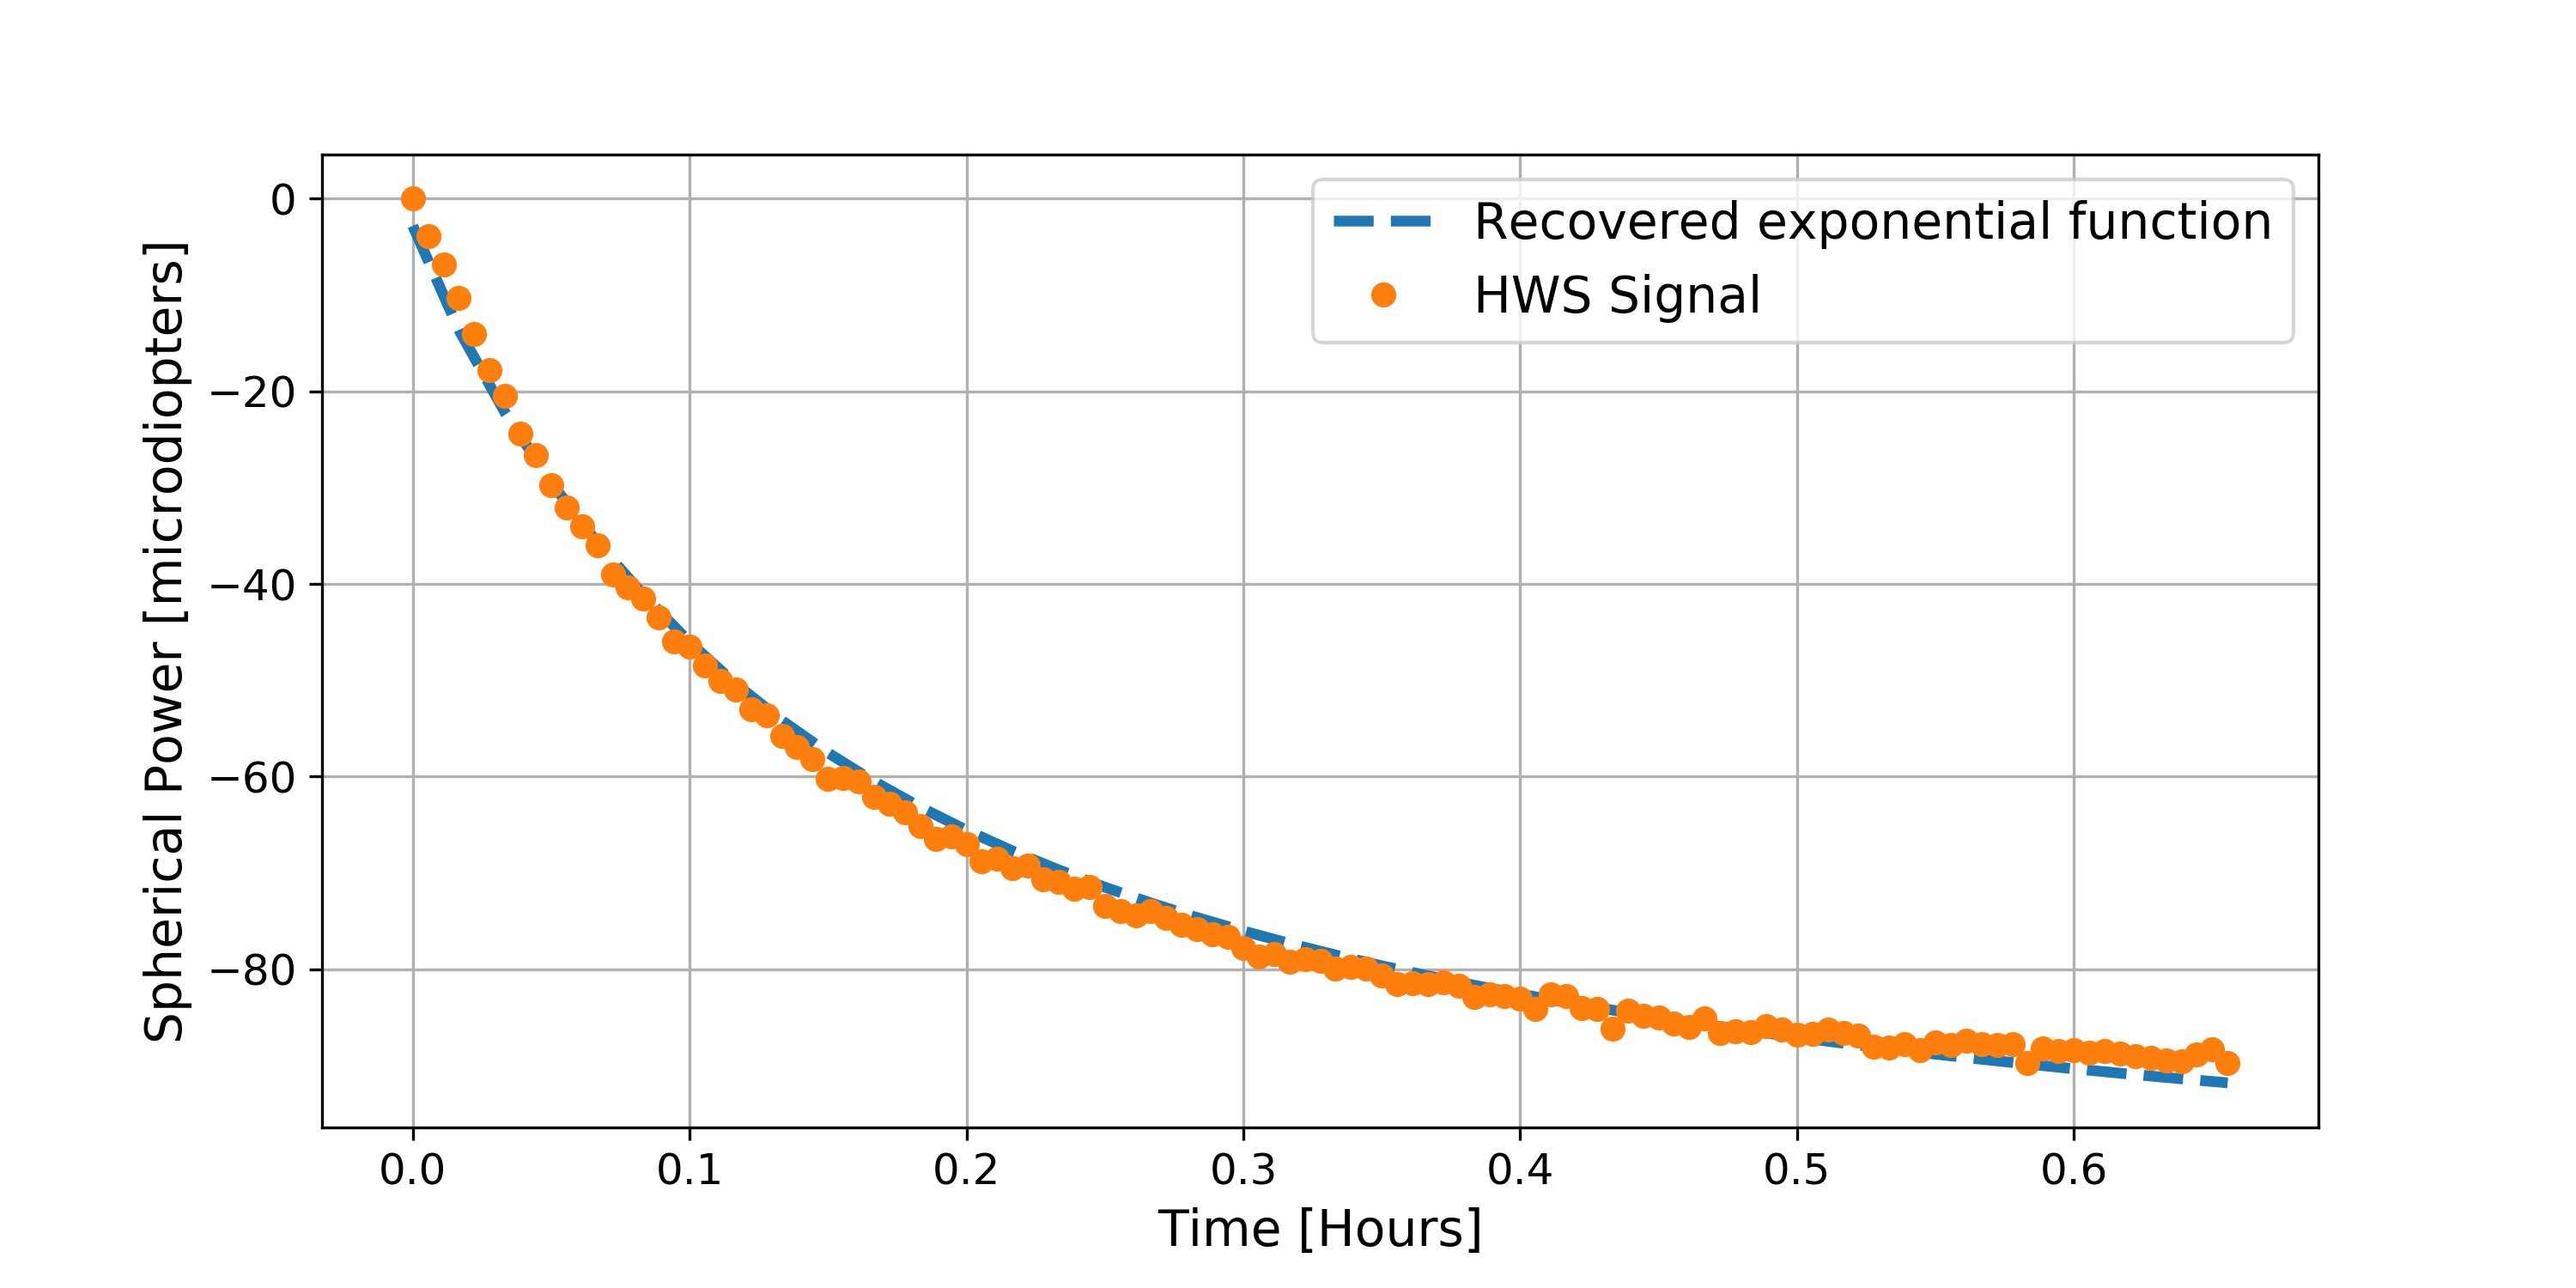
\includegraphics[width=\textwidth]{../Figures/MCMC_ITMY_ABS_FIT.png}
			\caption{ITMY absorption}
			\label{fig:itmy_abs}
		\end{subfigure}
		\caption[Thermal lensing as seen by the ITM Hartmann Sensors after a lock loss.]  
		{\textbf{Thermal lensing as seen by the ITM Hartmann Sensors after a lock loss.} A finite element simulation from COMSOL shows an impulse response which resembles an exponential decay can be linearized and fitted to the spherical power. The model assumes a beam size of 54 mm and 1 Watt of uniformly absorbed power then uses MCMC to fit the offset and scale to the data. Comparing ITMX and ITMY at Hanford shows a huge overall difference between the two optics, mostly due to the fact that ITMY has multiple point absorbers adding to the absorption estimate.  In addition, fitting ITMY data points with the model does not seem to agree very well which indicates extra physics that stems from non-uniform heating by a 54 mm beam.}
		\label{fig:hws_abs}
	\end{figure}
	
	\begin{figure}[!]
		\centering
		\begin{subfigure}[b]{0.5\textwidth}
			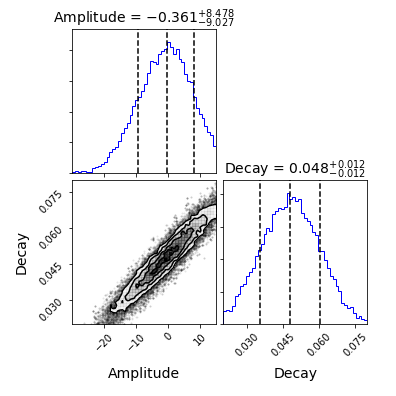
\includegraphics[width=\linewidth]{../Figures/MCMC_ITMX_abs.png}
			\caption{ITMX}
			\label{fig:mcmc_itmx_abs}
		\end{subfigure}%
		\begin{subfigure}[b]{0.5\textwidth}
			\includegraphics[width=\linewidth]{../Figures/MCMC_ITMY_abs.png}
			\caption{ITMY}
			\label{fig:mcmc_itmy_abs}
		\end{subfigure}
		\caption[Posterior distributions from fitting the Hartmann sensor spherical power.]  
		{\textbf{Posterior distributions from fitting the Hartmann sensor spherical power.}  
			Using the MCMC Hammer \cite{MCMC_Hammer} to fit the finite element model from Figure \ref{fig:hws_abs}, the two open parameters to solve for the decaying exponential is the amplitude and the decay rate which is related to the level of uniform absorption.}
		\label{fig:mcmc_hws_abs}
	\end{figure}
	
	\subsection{Ring Heater and CO$_2$ Laser Commissioning}\label{Sec:RH}
	To counteract the effects of interferometer heating, Advanced LIGO uses a ring heater \cite{ramette_analytical} \cite{wang_thermalmodel} which has two heating elements mounted on the suspension cage. Each of them are comprised of a semi-circular glass cylinder that is wrapped by nichrome wire, which has current running through the wire to radiate an annular heating pattern. The ring heaters will have two effects: it will induce a substrate lens and a radius of curvature change.  As shown in Section \ref{sec:hotcoldifo}, the carrier beam will not see the substrate lens but the radius of curvature difference will change the overall modal shape of the cavity.  Similar to the distortion derived in section \ref{sec:wf_dist} where the thermo-refractive effect dominates when dealing with a Gaussian beam, the same is true from the ring heaters.

	After using the Hartmann sensors to determine the absorption and pre-loading the ring heaters to compensate the interferometer lensing, the fact that the substrate is cold makes lock acquisition difficult.  Therefore, it is necessary to use CO$_2$ (Carbon Dioxide) lasers to mimic the interferometer's heating by delivering heat to the compensation plate.  The CO$_2$ lasers are located on each input test mass chamber and injected through a double zinc selenide viewport, then two steering mirrors direct the heating beam to the compensation plate of the reaction mass.  In initial LIGO, the CO$_2$ beams were injected onto the high reflectivity surfaces of the test masses which created both a radius of curvature on the cavity side and a thermo-refractive change in the substrate.  However, in advanced LIGO, the CO$_2$ lasers will only affect the substrate lensing.  Tuning the CO$_2$ power will have a dramatic effect on the interferometer auxiliary degrees of freedom because the sidebands get rejected by the arm cavity and only resonate in the recycling cavities.  The self-heating caused by the interferometer beam is assumed to have a Gaussian intensity profile, while the CO$_2$ heating beam is meant to have a uniform profile across the test mass surface which allows for a consistent phase distortion as a beam passes through the substrate.  Settings for the ITM ring heaters and CO$_2$ lasers are calculated in Figure \ref{fig:TCS_ITMs} based off the Hartmann measurements.  Adding the effect of pre-loading will inherently change the Gaussian mode overlap between the x-arm and y-arm.  Using equation \ref{gauss_power_ovl}, one can directly calculate the power overlap between a pre-loaded cavity and the original, as it turns out, the effect varies the overlap by less than $0.1\%$ so the addition of ring heater power for O3 will not change the modal contrast defect by much.
	
	Determining the ITM ring heaters and CO$_2$ power levels still leaves the end test mass ring heaters to be set.  In Figure \ref{fig:TCS_ETM}, the goal is to maintain the mode matching between the arms while simultaneously searching for the optimal overlap with the power recycling cavity.  This is done by determining the spatial mode overlap between all three cavities (XARM, YARM, and PRC). The linear portion of the graph shows a combination of common and differential adjustment of each ETM ring heater that keeps the mode matching between the arms at less than 1 ppm by calculating the Gaussian beam overlap.  Once that region is found where both arms are well mode matched, sampling the ara where there is maximal mode overlap with the power recycling cavity can be determined and is shown with contour plots. 
	
	\begin{figure}[!]
		\centering
		\begin{subfigure}[b]{1.0\textwidth}
			\centering
			\includegraphics[width=\textwidth]{../Figures/ITMX_TCS_Settings.png}
			\label{fig:TCS_ITMX}
		\end{subfigure}
		\hfill
		\begin{subfigure}[b]{1.0\textwidth}
			\centering
			\includegraphics[width=\textwidth]{../Figures/ITMY_TCS_Settings.png}
			\label{fig:TCS_ITMY}
		\end{subfigure}
		\caption[Calculated TCS settings to balance the substrate lens.]{
			\textbf{Calculated TCS settings to balance the substrate lens.}  The nominal circulating power denoted by the vertical blue line is a function of the input power, the recycling gain, and the arm cavity gain.  The nominal input power for O3 will be 50 Watts and the power recycling gain is around 45.  The arm cavity gain can be estimated by calibrating the transmitted power from each of the arms and is approximately 228.  The horizontal, dashed turquoise line represents the nominal substrate lens with a focal length of 50 km.  The total substrate thermal lensing from ring heaters, CO$_2$ lasers, and interferometer heating should sum up to the turquoise line.  The left column of graphs show the necessary ring heater and CO$_2$ laser powers required to compensate the interferometer heating. The left column of graphs show the required CO$_2$ power if the ring heaters are constantly energized during lock acquisition because their thermal time constants are on the order of a few hours.  The spread in the estimates stem from uncertainty in the uniform absorption which is crucial in determining the correct TCS settings
		}
		\label{fig:TCS_ITMs}
	\end{figure}
	
	\begin{table}[]
		\centering
		\begin{tabular}{|l||r|r|r|}
			\hline
			\hline
			& \multicolumn{1}{c|}{Substrate} & \multicolumn{1}{c|}{HR surface} & \multicolumn{1}{c|}{Compensation Plate} \\ \hline
			Self Heating & *4.9e-4                       & *-3.6e-5                        & N/A                                     \\ \hline
			Ring Heater  & -9.0e-6                       & *9.9e-7                         & N/A                                     \\ \hline
			CO$_2$x         & N/A                            & N/A                             & 1.5e-5                                  \\ \hline
			CO$_2$y         & N/A                            & N/A                             & 2.5e-5                                  \\ \hline
		\end{tabular}
		\caption[Single pass actuator lensing calibrations for aLIGO TCS in micro-diopters/Watt.] 
		{\textbf{Single pass actuator lensing calibrations for aLIGO TCS in micro-diopters/Watt.} The asterisks indicate the values are extracted from a model and the measured values use the Hartmann sensors which cannot distinguish between surface and substrate lensing, however, the latter is larger by an order of magnitude.  CO$_2$x and CO$_2$y were measured to be different in their actuation strength which could stem from either misalignment or a misplaced central mask.  The uncertainty is expressed by the last digit available.
		}
		\label{tbl:Actuaor_calibs}
	\end{table}
	
	\begin{figure}[!]
		\centering
		\includegraphics[width=1.0 \textwidth]{../Figures/ETM_TCS_Settings.png}
		\caption[Mode matching the arm cavities to the power recycling cavity.]{
			\textbf{Mode matching the arm cavities to the power recycling cavity.}
		}
		\label{fig:TCS_ETM}
	\end{figure}
\clearpage
\section{Point Absorbers}\label{sec:point_absorbers}
	Up till now, all actuators models, and measurements assumed uniform absorption across the optics which results in second order Hermite-Gauss coupling with the fundamental Gaussian beam .  As it turns out, the instrument is not so simple. One of the main successes for the Hartmann Wavefront Sensors have been the ability to find excess absorption due to point absorbers on the high reflectivity surfaces of the test masses.  During the second observation run (O2), there was an absorber found on ITMX that made increasing the input power past 30 watts extremely difficult and futile because of increased coupling intensity noise into DARM. The exact origin of these point absorbers is still an active area of research but incursions into the vacuum system will always pose a risk of spreading particulate on the HR surfaces.

	\textbf{\emph{Part way into commissioning for O3, another point absorber on ITMY was detected that showed similar characteristics.}}  Since their spatial frequencies are much higher than the uniform absorption, many of the models for scattered power and thermal effects require significant adjustment to predict the interferometer behavior.  To decompose the differential phase map into the Hermite Gauss basis requires a relatively high order and makes full interferometer simulations very difficult.  For example, FINESSE calculations on a laptop tend to become unwieldy at around $n+m = 6$.  The high spatial frequency of point absorbers affects the HWS's ability to properly evaluate a singular thermal lens from the interferometer, therefore changing the estimated absorption.  
	
	A way to separate the point absorber effect from uniform absorption could be considering the temporal effects which quadratically depend on the point absorber size. The thermo-refractive transient solution found in Vinet \cite{Vinet_Thermal_Issues} has the form
	\begin{equation}\label{Thermal_Dist_time}
	Z_{\text{TR}}(t)   \propto 1-\exp{-t/ \tau}
	\end{equation}
	where $\tau = \frac{\rho C w_\text{pa}^2}{3 \kappa} $ is the characteristic time constant that depends on the beam size $w_\text{pa}$, the thermal conductivity $\kappa$, the specific heat $C$ and the material density $\rho$.  A simple model can consist of two beams with different sizes which will have separate time constants.  Another interesting way of characterizing what can be compensated for O3 could be to Fourier transform the optical path distortion and low pass the high spatial frequency components with a Gaussian filter. The cut-off frequency can be estimated by the approximate point absorber size (10-20 mm).  Of course, early detection and replacement of an optic may be the most efficient way to avoid custom thermal compensation.  Figure \ref{fig:3d_HWS_plot} shows a comparison between ITMX and ITMY while the interferometer is increasing input laser power from 2 to 30 Watts.  Within the first few hundred seconds, the point absorbers begin showing up in the optical path distortion map.
	
	There are two main parts which allow point absorbers to adversely affect interferometer performance.   The first is scattering from the arm cavity that takes away carrier light and couples to higher order modes, and secondly, the thermal lens in the substrate distorts the power recycling cavity for the sideband build ups dramatically.
	
	
	An interesting coupling that was discovered which the point absorbers could be responsible for is higher order mode 9 Mhz leakage through the OMC.  Generally, the OMC is very good at rejecting both the sidebands and first few higher order modes but the addition of point absorbers couples greater spatial frequencies than anticipated.  Careful analysis by Koji Arai \cite{9rin} shows the Hanford OMC can allow some 9th order Hermite Gauss modes from the 9 MHz sidebands onto the OMC DCPDs.  This coupling should provide a decent metric for indicating the point absorber's induced noise on the interferometer. 
	
	During commissioning periods, the highest starting priority is to achieve full resonance as quickly as possible, and that is easier to accomplish using approximately 2 W of input laser power. This requires locking the arm length stabilization (ALS) system with 532 nm, the vertex degrees of freedom (DRMI) and complete the common arm length (CARM) transition. Additionally, closing all angular degrees of freedom (ASC) will take a lot of time and energy.  If major upgrades or fixes have occurred such as replacing main test masses then all the prior steps require many months of commissioning.  Generally, vacuum incursions into the main vertex cost the most time and money because of the large volume needing to be pumped.  All this is to say: the earlier point absorbers are detected, the better.  However, this requires a high level of arm power which historically has come much later on the road to nominal low noise.  In Figure \ref{fig:HWS_spectra}, the signal-to-noise ratio is 10 at 0.01 Hz for 37.5 mW of absorbed power which means the circulating arm power must reach at least 75 kW  (assuming absorption is approximately 0.5 ppm) to be detectable within the time constant of point absorbers.
	
	The power recycling gain for a single arm is described by
	\begin{equation}
	g_{\text{PRC'}} = \bigg\vert \frac{t_{\text{p}}}{1-r_p r_1 \frac{1}{2}} \bigg\vert^2 \approx 0.12
	\end{equation}
	where the factor of 0.5 comes from the main beamsplitter.  This is much different than a gain of 45 for a full interferometer but it is still a factor of 4 larger than direct transmission through the PRM. So with a single power recycled arm cavity the expected circulating power absorbed on the HR surface of the test masses is
	\begin{equation}
	\begin{aligned}
	P_\text{1-ARM} 	&= P_{\text{in}} * g_{\text{ARM}}  * g_{\text{PRC'}} * \epsilon_a \\
					&\approx 0.94 \; mW \; \bigg[\frac{P_{\text{in}}}{70 \, \text{Watts}}\bigg] \; \bigg[\frac{g_{\text{ARM}}}{ 225 }\bigg] \;  \bigg[\frac{g_{\text{PRC'}}}{ 0.12 }\bigg] \; \bigg[\frac{\epsilon_a}{0.5 \, \text{ppm}}\bigg]
	\end{aligned}
	\end{equation}
	where the coefficient $\epsilon_a$ is the estimated absorption from a point absorber.  Using $ D_{\text{sub}} \approx 487 \frac{\mu \text{D}}{1 \; \text{Watt}}$ as the modeled conversion from absorbed power to steady-state spherical thermal lensing, the expected substrate lensing in units of micro-diopters [$\mu \text{D}$] is
	\begin{equation}
	S_\text{1-ARM} = P_\text{1-ARM} *  D_{\text{sub}} \approx 0.46 \; \mu\text{D}
	\end{equation}
	 which is not detectable by the current Hartmann sensors but the overall effect will be dependent on the absorption coefficient. Commissioning and installation schedules are ever-changing entities and there have been times when the end stations are not ready for integration simultaneously. This provides a window where only single arm commissioning is available so this method may be able to detect the existence of point absorbers much sooner.
	 
	 \indent Once these anomalies are found, the question remains, what can be done?
	 
	 One consideration is a complete re-design of Thermal Compensation to account for higher frequency spatial corrections. There are already custom masks at Hanford which are designed to smooth the optical path distortion in the substrate and can be implemented with the CO$_2$ lasers on the compensation plate to increase the sideband build ups, which is one of the biggest difficulties associated with point absorbers.  However, this does not solve the fundamental problem of losing power recycling gain due to power scattering where the quadratic losses of the arm cavity set an upper limit for increasing power.  Another way to avoid these effects is to move the beam spot away from the point absorber on the HR surface but it must be sufficiently far or the odd higher order modes will couple very strongly with asymmetry. These two strategies are not necessarily orthogonal since moving the spot position changes the required correction mask.
	 
	 In terms of noise, the 9 MHz RIN coupling to the OMC DCPDs could be reduced by changing the OMC transverse mode spacing by locking on a different carrier resonance a free spectral range away.  The introduction of a well-tuned custom mask should also reduce higher order mode content in the recycling cavities.
	 
	 \begin{figure}[t!]
	 	\centering
	 	\includegraphics[width=0.4\textheight]{../Figures/1231726400_3d_200dur_30W_ITM.png}\quad
	 	\includegraphics[width=0.4\textheight]{../Figures/1231726400_3d_500dur_30W_ITM.png}\quad
	 	\includegraphics[width=0.4\textheight]{../Figures/1231726400_3d_1000dur_30W_ITM.png}\quad
	 	\caption[Comparing 3-D plots of the optical path distortion for ITMX and ITMY test masses after powering up the interferometer.]  
	 	{\textbf{Comparing 3-D plots of the optical path distortion for ITMX and ITMY test masses after powering up the interferometer.}
	 		The horizontal axes represent the test mass coordinates as seen on the Hartmann sensors and the vertical axis is the optical path distortion in units of nanometers. The color map is scaled for each plot and is meant to show particularly hot areas and roughly compare the high frequency spatial distribution of point absorbers. Plots in the left column (ITMX) have smooth spatial features that stem from uniform absorption and the effects are not prominent till after approximately 500 seconds.  In contrast, plots in the right column (ITMY) have very sharp spatial features which already rise above the floor at 200 seconds into powering up.  Comparing the overall surface deformation on the same scale, the difference between ITMX and ITMY is striking and it is clear how an interferometer with point absorbers on the surface will struggle to increase powers above 200 kW within the arm cavities.
	 	}
	 	\label{fig:3d_HWS_plot}
	 \end{figure}

	\begin{sidewaysfigure}[t!]
		\centering
		\begin{minipage}{0.5\textheight}
			\centering
			\includegraphics[height=0.5 \textheight]{../Figures/Simplified_PRC_ARM_etm_abs.png}
		\end{minipage}\hfill
		\begin{minipage}{0.5\textheight}
			\centering
			\includegraphics[height=0.5 \textheight]{../Figures/Simplified_PRC_ARM_itm_abs.png}
		\end{minipage}
		\caption[Interferometer DC powers as a function of round trip arm loss and test mass absorption.]  
		{\textbf{Interferometer DC powers as a function of round trip arm loss and test mass absorption.}
			Simplifying the power recycling cavity and a combined arm model to understand the powers as a function of loss has a few advantages with regards to computational time and the results are easier to conceptually understand.  Here, absorption changes the radius of curvature and substrate thermal lens which results in some mode mismatch while the round trip loss takes into account the rest of the higher order modes from point absorbers.  The ITM absorption has a much larger effect on the overall power recycling gain loss by almost a factor of 3 compared to ETM absorption.  Of course, the simplified model will fall short in describing effects on the antisymmetric signals of the full interferometer.
		}
		\label{fig:simple_prc_arm}
	\end{sidewaysfigure}

\clearpage

\section{Higher Power Operation}
	The goal for O3 is 150 kW of circulating power in the arms. With the sensors and tests described in the preceding sections, a cohesive plan to pre-load the interferometer was implemented in order to achieve stable higher power operation in the detectors.  Generally, the Thermal Compensation System has two goals: Firstly, the actuators are used to pre-load the test masses with heat in anticipation of the lensing due to the interferometer while operating at full lock and higher power.  Secondly, the amount of mode-matching between the coupled cavities must be optimized in order to achieve the best sensitivity.  Using the absorptions measured in Figure \ref{fig:hws_abs}, it is possible to estimate the total amount of lensing from self-heating as a function of input power (see Figure \ref{fig:TCS_ITMs}).

	In principle, the Hartmann measurements of absorbed power should provide sufficient information to pre-load the interferometer in anticipation of 50 W of input power.  The biggest difficulty associated with implementing this thermal compensation scheme was consistently locking DRMI in high micro-seismic conditions. This could be attributed to misalignment of CO$_2$ lasers to the test masses, which were initially aligned using the Hartmann sensors and double-checked by cycling the lasers on/off to measure the single bounce interferometer beam deflection at the anti-symmetric port. At Hanford, this difficulty for reliably locking the interferometer forced a reduction in pre-loading, so with the combination of estimates provided by the Hartmann Sensors and experimentation with the CO$_2$ power levels at each stage of increasing the PSL power, the interferometer is able to consistently lock at 30 Watts of PSL input power and $\approx 140 \; kW$ of circulating arm power. 
	
	\begin{figure}[t!]
	\centering
	\includegraphics[width=0.75 \textwidth]{../Figures/POP_18dive.png}
	\caption[Model of POP-18 as a function of differential thermal lensing using FINESSE.]  
	{\textbf{Model of POP-18 as a function of differential thermal lensing using FINESSE.}
		The horizontal axis is differential lensing between the ITMX/ITMY substrates and the vertical axis represents the normalized power when locked with nominal mode matching.  Even with modest differential lensing (10 microdiopters), the buildup drops by 20 percent and eventually the simulation has trouble maintaining resonance, similar to the actual interferometer.
	}
	\label{fig:POP18}
	\end{figure}

	During the early phases of commissioning for higher power at Hanford, most of the lock losses occurred when the 18 MHz sidebands in transmission at PR2 (POP-18) would fall below a certain threshold level of approximately 70\% of buildup compared to locking at 2 W of input power.  This effect was not observed at Livingston and can be attributed to the point absorber that uniquely contaminated H1-ITMY.  To study the effects of differential uniform lensing in an interferometer, FINESSE is able to simulate the POP-18 signal at the power recycling pick-off port demodulated at 18 MHz which shows the sideband power buildup in the power recycling cavity (see Figure \ref{fig:POP18}). In this particular simulation the differential lensing requires finding a new operating point to continually lock the longitudinal degrees of freedom.  Additionally, the simulated sensors which are used to maintain resonance and measure the RF power need to be re-phased; this agrees with the analytical calculation mentioned in Section \ref{Sec:TL_lensing} where the carrier power recycling gain is not as adversely affected by the substrate thermal lens compared to the sideband fields.
	
	In the ideal mode matching scenario, the carrier and sidebands resonate differently in the power recycling cavity; where the 9 MHz modulation sidebands has approximately a factor of 10 larger finesse than the carrier \cite{kiwamu_freq1}.  However, this assumes a lossless interferometer and needs to be revisited in the presence of substrate thermal lensing.   As with all Pound-Drever-Hall locking, an error signal relies on the static and varying field accumulating different phases to lock the cavity. As lensing causes more losses for the sideband compared to the carrier, the difference in accumulated phase between the two fields is reduced hence the optical gain starts to diminish.  For the current Advanced LIGO configuration, all vertex degrees of freedom (PRCL, SRCL, MICH) utilize the POP port for their error signals shown in Figure \ref{fig:vertex_OLTF}. The degradation can be estimated by injecting a dither line into each degree of freedom and digitally demodulating the respective sensors at the excitation frequency, see Figure \ref{fig:POP18_POP90}.  This provides insight on how much the optical gain/phase shifts as a function of heating.  When powering up to 30 Watts, the loss of optical gain in PRCL is almost 80\% with a 10 degrees phase shift, which enough to drive the system towards an unstable loop.  This can be compensated by adjusting the digital gain but that fix is only temporary because the problem stems from an optical loss so eventually, the error signal will have no linearity about the zero-point.  Alternatively, searching for optimal thermal compensations settings to undo these losses can be very time consuming because of the long thermal time constants and in the case of point absorbers, the current thermal compensation system is not designed to correct the high spatial frequencies.  As previously mentioned, one of the main limiters to higher power operation will be reducing the optical loss from mode mismatch.

	\begin{figure}[t!]
		\centering
		\includegraphics[width=0.75 \textwidth]{../Figures/MeasuredVertexOLF.png}
		\caption[Vertex open loop transfer functions while in Nominal Low Noise.]  
		{\textbf{Vertex open loop transfer functions while in Nominal Low Noise.}
			The nominal UGF for PRCL is around 45 Hz.
		}
		\label{fig:vertex_OLTF}
	\end{figure}
	
	\begin{figure}[t!]
		\centering
		\includegraphics[width=1.0 \textwidth]{../Figures/PRCL_EXC_LSC-POP_A_RF9_I.png}
		\includegraphics[width=1.0 \textwidth]{../Figures/SRCL_EXC_LSC-POP_A_RF45_I.png}
		\includegraphics[width=1.0 \textwidth]{../Figures/MICH_EXC_LSC-POP_A_RF45_Q.png}
		\caption[Measuring vertex optical gains as a function of heating.]  
		{\textbf{Measuring vertex optical gains as a function of heating.}
		At time t=0, the power begins increasing from 2 watts of input power to 20 watts. In PRCL, there is a reduction to 80\% of the starting magnitude and 7.5 degrees of phase rotation with the first power increase. At 0.9 hours, the input power goes from 20 to 30 watts and the magnitude drops to about 30\% of the original gain which results in a lock loss.  As for the SRCL and MICH degrees of freedom, there are slight changes first power increase but not nearly as bad as PRCL.
		}
		\label{fig:POP18_POP90}
	\end{figure}

\clearpage

\section{Mode Matching from the OPO to the OMC}
	As mentioned in Chapter 2, one of the main limitations to effective squeezing is mode mismatch which needs to be characterized carefully.  Generally, the mode exiting the OPO and OMC cavities are accurately determined from design values but the path lengths and mode profile was measured and the results are presented in this section.
	
	\begin{figure}[]
	\centering
	\includegraphics[width=0.7\textwidth]{../Figures/Lens_Closest_to_OPO.png}
	\includegraphics[width=0.7\textwidth]{../Figures/Lens_in_Center_Position.png}
	\includegraphics[width=0.7\textwidth]{../Figures/Lens_Furthest_from_OPO.png}
	\caption[OPO to OMC cavity scanning for various Lens2 positions.]  
	{\textbf{OPO to OMC cavity scanning for various Lens2 positions.}  The top figure has the lens closest to the OPO along the propagation axis, the middle figure represents Lens2 at half the actuation range and the bottom figure shows the lens furthest from the OPO.  During this time, the OMC ASC control loops were closed on the reflected QPDs to minimize the odd order mode coupling.  
	}
	\label{fig:OPO_to_OMC_scan}
	\end{figure}

	Using the OMC as an optical spectrum analyzer is one simplest methods for understanding the mode matching coming out of the interferometer.  In a single bounce configuration, measuring the ratio between the second order mode and the fundamental gives a first look at the limit of matching.  Similar techniques can be used with the squeezed beam as well and during commissioning of the squeezer, a mode mismatch between 12-17\% was observed which led to a re-design of the OPO to OMC optical path.  Figure \ref{fig:OPO_to_OMC_scan} shows the results for scanning the OMC length using PZT2 with the  ASC control loops closed on the reflected QPDs to minimize odd-order mode coupling.  The measurements were taken in-air which made the results rather noisy so before the peak-finding algorithm tries to fit the 00 or 02 modes, the data is low-passed with a corner frequency of 1kHz.
	
	Using a well-calibrated mode profiler that measures beam sizes along the propagation axis is the most direct way of determining OPO to OMC mode matching.  This method can also predict the actuator Gouy phase of the second lens after the OPO, which is on a translation stage with approximately 4 centimeters of range. Generally, the length measurement between optics is the largest systematic error especially in the near-field where beam sizes do not change very much as a function of $\hat{z}$.  In addition, places to put a beam profiler become very limited as HAM6 becomes crowded with optical components.  In preparation for squeezing in Advanced LIGO, the mode matching from the OPO to OMC was measured and found to be approximately 88\% at best. When implementing a telescope with fast lenses, the distances between optics must be stringently characterized but the OPO platform is very crowded along the output path so it was very difficult to accurately measure the path lengths with a ruler.  Between the second lens and ZM1, the table is much clearer and by removing Lens2, the Gouy phase is approximately in the far-field which means the distance measurements can be more easily measured as a function of beam size.  Figure \ref{fig:OPO_to_ZM2} shows the results of characterizing the OPO output mode as it enters HAM5 by removing Lens2, a fit constrains the Lens1 positioning and the OPO mode is assumed from its design document \cite{Oelker_FD_sqz}.
	
	With the poor mode matching shown in Figure \ref{fig:OPO_to_OMC_Old}, the fast telescope lenses needed to be replaced, or otherwise, risk being the limit to effective squeezing for O3.  The available range in the translation stage did not allow for increased matching and the crowded OPO platform did not permit coarse moves of Lens1. In addition, moving the translation stages for Lens2 closer to the OPO cavity does not gain any extra mode overlap.  The next option was replacing the lenses with a solution which did not incorporate large actuation range but was more suited for mode matching.  There were a few clean lenses available that provided the right solution but greatly reduced the translation stage efficacy, on the other hand, this made the telescope placement much more robust to path length errors which is the original problem to begin with.  The new model is shown in Figure \ref{fig:OPO_to_OMC_New} where the lenses are now  $f^{\text{new}}_{\text{Lens1}} = 250$ mm and $f^{\text{new}}_{\text{Lens2}} = 350$ mm where Lens1 is closer to the OPO output.   The calculated overlap integral between the expected OMC mode and the squeezer is on the order of 99\% with very little sensitivity in the Lens2 positioning as expected.  Follow up measurements with OMC scans in-vacuum indicate approximately 95\% mode matching between the OPO to SRM and back to the OMC, this is due to the astigmatism mentioned previously that is still prevalent after changing the lenses.  However, the mode matching from the OPO to ITMs and back to the OMC shows 99\% mode matching with the new lens configuration \cite{modematch99} which is effectively the path of squeezed light.  It is important to note that measurements taken in-vacuum had pre-loaded TCS settings in anticipation for 50 W.
	
	For future implementations of high sensitivity telescopes, length measurements between optics will need to be more stringently constrained with specialized tools such as laser range finders or mechanical jigs while simultaneously re-confirmed with profile scans to understand the laser beam entering the interferometer.  Distances between optics were the largest source of uncertainties in these measurements so understanding the optical path length will help curb the systematic errors.
	
	\begin{figure}[]
		\centering
		\includegraphics[width=0.8 \textwidth]{../Figures/OPO_to_ZM2_fit.png}
		\caption[Mode measurement from the OPO.]  
		{\textbf{Mode measurement from the OPO.}
			The results without Lens2 are shown in black for two transverse directions (x/y) and constrain the distance of Lens1 relative to the OPO output.  Then, Lens2 is replaced back in its original position on a translation stage at half the range and measurements were taken in order to constrain the distance between Lens1 and Lens2.  The beam sizes were fit to find the Gaussian q-parameter entering HAM5. There is some slight deviation in the transverse directions after Lens2, possibly from misalignment of the lens.  This method seems to provide a good model of what beam is being injected from the squeezer side.
		}
		\label{fig:OPO_to_ZM2}
	\end{figure}
	\begin{figure}[t!]
	\centering
	\includegraphics[width=0.8 \textwidth]{../Figures/OPO_to_OMCREFL_Oldlenses.png}
	\caption[Projecting the modes from the squeezer to the OMC.]  
	{\textbf{Projecting the modes from the squeezer to the OMC.}
		Determining the actuation range with the translation stage using the as-installed focal lengths, $f_{\text{Lens1}} = 111$ mm and $f_{\text{Lens2}} = 334$ mm, showed that the mode matching into the OMC was at most 80\% with various translation stage positions with ``Close" referring to the position of Lens2 relative to the OPO cavity.  Here, crosses represent the transverse-x direction and pluses denote the transverse-y orientation.  One very interesting feature is that the astigmatism as measured seems to be worse after re-entering HAM6 from HAM5 and is not explainable by the slight deviations shown in Figure \ref{fig:OPO_to_ZM2}, so it is possible that some sort of clipping occurs while propagating through the main output Faraday isolator.  Near the OMC waist, the predicted mode shapes for different translation stage positions agree with the measured beam sizes and power overlaps were confirmed to be accurate with OMC scans to within a percent.
	}
	\label{fig:OPO_to_OMC_Old}
	\end{figure}

	\begin{figure}[t!]
	\centering
	\includegraphics[width=0.8 \textwidth]{../Figures/OPO_to_OMCREFL_Newlenses.png}
	\caption[Repeated measurements with new lenses.]  
	{\textbf{Repeated measurements with new lenses.}  The model tries a few different lens solutions and settles on $f^{\text{new}}_{\text{Lens1}} = 250$ mm and $f_{\text{Lens2}} = 350$ mm, which severely limits the actuation range.  However, it shows approximately 97\% mode matching for the fitted transverse-y data and 92\% for the transverse-x data.  Astigmatism which was already shown in Figure \ref{fig:OPO_to_OMC_Old} is still prevalent here and brings the average mode matching to 95\% from the OPO to OMC in the single bounce configuration.
	}
	\label{fig:OPO_to_OMC_New}
	\end{figure}
\chapter{Solutions for Detector Upgrades} 
A solution to the current mode matching situation will be solved by further expanding active wavefront control described in Section \cite{AWC_current}. A full modal picture, sensors and actuator
	\section{Sensors}
* Bullseye photodetectors

* Operation: range (in terms of watts and percentage mismatch)


	\section{High Sensitivity Telescope}
	* Translation stages: General principles, rigging, sensitivity
	
	* Mechanical description (Solidworks designs)
	
	* Constraints (range, vacuum, alignment, integration)

	* Electronics 
	
	* Software
	
	*Implementation: rigg something better, in situ measurements.
	
	\section{A Global Active Wavefront Control Scheme}
	To truly implement a system that solves the mode matching challenges presented in LIGO, an active control scheme that implements both sensors and actuators will be required to span the degrees of freedom that are present in the interferometer.
	
	\subsection{Hard and Soft Mode Matching}
	Similar to the wavefront sensors already being used in LIGO at the time of this writing, the active wavefront system should be able to rotate the phase of their actuators and sensors to the common and differential basis.  Also, the extra two degrees of freedom required are the hard and soft modes for thermal lensing which curve the ITMs and ETMs in a way which vary the waist size and position orthogonally. 
\begin{appendices}

	\chapter{Resonator Formulas} \label{FPappendix}
	Equation \ref{gfactor} describes the stability condition for a two mirror Fabry-Perot cavity, but is worthwhile to derive the criterion for geometric stability from the ray matrix tools commonly used in optics. The alignment of two plane waves traveling in space can differ by two quantities: the axial and angular separations,  $y$ and $\theta$, respectively.  These two quantities can be transformed via these optical matrices:
	
	Lens:
	\begin{equation} \label{lens}
	\hat{F_i} = 
	\begin{pmatrix}
		1				&0			
	\\ 	-\frac{1}{f_i}	&1
	\end{pmatrix}
	\end{equation}
	
	Curved Mirror:
	\begin{equation} \label{mirror}
	\hat{M_i} = 
	\begin{pmatrix}
		1				&0			
	\\ 	\frac{2}{R_i}	&1
	\end{pmatrix}
	\end{equation}
	
	Space:
	\begin{equation} \label{space}
	\hat{D_i} = 
	\begin{pmatrix}
		1	& d_i		
	\\ 	0	&1
	\end{pmatrix}
	\end{equation}
	Using these matrices, the periodic Fabry-Perot with two mirrors can be represented by the matrix,
	\begin{equation}
	\begin{pmatrix} y_{m+1} 
	\\ \theta{m+1}
	\end{pmatrix}
	= \hat{M}_{FP} \begin{pmatrix} y_{m} 
	\\ \theta{m}
	\end{pmatrix}
	\end{equation}
	where 
	\begin{equation}
	\hat{M}_{FP} = \hat{M_i} \hat{D_i} \hat{M_i} \hat{D_i}
	\end{equation}
	is the optical transfer matrix.  The goal is to find a geometric condition that is dependent on the optical transfer matrix which keeps the axial displacement from diverging.
	\begin{equation}
	\begin{pmatrix} y_{m+1} 
	\\ \theta{m+1}
	\end{pmatrix}
	= 
	\begin{pmatrix}
		A	&B		
	\\ 	C	&D
	\end{pmatrix}
	\begin{pmatrix} y_{m} 
	\\ \theta{m}
	\end{pmatrix}
	\end{equation}
	which means
	\begin{subequations}
	\begin{equation}
	\theta_m = \frac{y_{m+1} - A \, y_m}{B}
	\end{equation}
	\begin{equation}
	\theta_{m+1} = \frac{y_{m+2} - A \, y_{m+1}}{B}
	\end{equation}
	\end{subequations}

	Solving for $y_{m+2}$
	
	\begin{equation}
	y_{m+2} = (A+D) \, y_{m+1} - \text{det}(\hat{M}_{FP}) y_m
	\end{equation}
	
	Assuming a geometrical solution where $y_m = y_o h^m$ and plugging into the equation above, 
	\begin{equation}
	h^2 = (A+D) \, h - \text{det}(\hat{M}_{FP})
	\end{equation}
	which is a quadratic equation that has two solutions and can be further simplified if the index of refraction for the entire system remains constant such that $\text{det}(\hat{M}_{FP}) =1 $.  Plugging back into $y_m$ and doing some algebra
	\begin{equation}
	y_m \propto \text{sin}(m \phi )
	\end{equation}
	where $\phi =\text{cos}^{-1} (\frac{A+D}{2})$, which is also referred to as the round trip Gouy phase of the cavity.  In order for $y_m$ to be harmonic instead of hyperbolic and hence confined, this condition must be met
	\begin{equation}
	\frac{\vert A+D \vert}{2} \leq 1
	\end{equation}
	
	By actually calculating the terms of $\hat{M}_{FP}$ and doing even more algebra, it is clear that 
	\begin{equation}
	0 \leq \bigg(1-\frac{L}{R_1}\bigg) \bigg(1-\frac{L}{R_2}\bigg) \leq 1
	\end{equation}
	which is what was stated in equation \ref{gfactor}. There is a simpler and less algebraic way to reach the same conclusion by looking at the Rayleigh range of a finite Gaussian beam for a simple cavity.   In Table II of Kogelnik and Li \cite{Kogelnik}, there is an expression for the Rayleigh range
	
	\begin{equation}
	\begin{aligned}
	z_{R}^2 &= \frac{L (R_1-L) (R_2-L) (R_1+R_2 - L) }  {(R_1+R_2-2L)^2}\\
			&= \frac{g_1 g_2 (1-g_1 g_2}{(g_1 - g_2 - 2 g_1 g_2)^2}
	\end{aligned}
	\end{equation}
	If the Rayleigh range is a real number, then once again, equation \ref{gfactor} must be true.
	
	\chapter{Hermite Gauss Normalization}
	According to equation \ref{HG}, the higher order modes in the Hermite Gauss basis has the intensity profile,
	\begin{equation}
		I_{mn} (x,y,z) = \vert A_{mn} \vert^2 \bigg[ \frac{W_0}{W(z)} \bigg]^2  \mathbb{G}^2_n\Bigg( \frac{\sqrt{2}x}{W(z)} \Bigg) \mathbb{G}^2_n\Bigg( \frac{\sqrt{2}y}{W(z)} \Bigg)
	\end{equation}
	It is useful to normalize the first few lowest order modes with respect to the total optical power since the Gaussian beam will couple to them the most due either misalignment or mode mismatch as seen in section []. In one dimension, the total optical power for the first 3 modes are
	\begin{equation}
	\label{HGNormalInt1D}
	\begin{aligned}
		P_{0}(x,y,z) 	& 	=	\int_{-\infty}^{\infty}  \vert A_{0} \vert^2   \bigg[ \frac{W_0}{W(z)} \bigg] e^{-2x^2/w^2(z)} dx	&
	\\	P_{1}(x,y,z)	&	=	\int_{-\infty}^{\infty}  \vert A_{1} \vert^2  \bigg[ \frac{W_0}{W(z)} \bigg] \frac{8x^2}{w^2(z)} 	
								e^{-2x^2/w^2(z)}dx &
	\\	P_{2}(x,y,z)	&	= 	\int_{-\infty}^{\infty}  \vert A_{2} \vert^2   \bigg[ \frac{W_0}{W(z)} \bigg] \bigg(\frac{8x^2}{w^2(z)}	-2\bigg)^2e^{-2x^2/w^2(z)}dx
	\end{aligned}
	\end{equation}
	In two dimensions, the total optical power for the first 3 modes are
	\begin{equation}
	\label{HGNormalInt2D}
	\begin{aligned}
		P_{00}(x,y,z) 	& 	=	 \int_{-\infty}^{\infty} \int_{-\infty}^{\infty}  \vert A_{00} \vert^2   \bigg[ \frac{W_0}{W(z)} \bigg]^2 e^{-2x^2/w^2(z)}e^{-2y^2/w^2(z)} dx dy&
	\\	P_{10}(x,y,z)	&	=	\int_{-\infty}^{\infty} \int_{-\infty}^{\infty}  \vert A_{10} \vert^2  \bigg[ \frac{W_0}{W(z)} \bigg]^2 \frac{8x}{w^2(z)} e^{-2x^2/w^2(z)}e^{-2y^2/w^2(z)} dx dy&
	\\	P_{20}(x,y,z)	&	= 	\int_{-\infty}^{\infty} \int_{-\infty}^{\infty}  \vert A_{20} \vert^2   \bigg[ \frac{W_0}{W(z)} \bigg]^2 \bigg(\frac{8x^2}{w^2(z)} - 2\bigg)^2 e^{-2x^2/w^2(z)}e^{-2y^2/w^2(z)} dx dy
	\end{aligned}
	\end{equation}
	By setting the equations above to unity, the normalization factors become
	\begin{equation}
	\begin{aligned}
		A_{0} &	= \bigg( \frac{2}{\pi w_0^2} \bigg)^{1/4} 
	\\	A_{1} &	= \bigg( \frac{2}{\pi w_0^2} \bigg)^{1/4} \frac{1}{\sqrt{2}}
	\\	A_{2} &	= \bigg( \frac{2}{\pi w_0^2} \bigg)^{1/4} \frac{1}{\sqrt{8}}
	\end{aligned}
	\end{equation}
	
	\begin{equation}
	\begin{aligned}
		A_{00} &	= \sqrt{\frac{2}{\pi w_0^2}}
	\\	A_{10} &	= \sqrt{\frac{1}{\pi w_0^2}}
	\\	A_{20} &	= \sqrt{\frac{1}{4\pi w_0^2}}
	\end{aligned}
	\end{equation}
	
	\chapter{Bullseye and Quadrant Photodiode Characterization}\label{BPDchar}
	Both RF and DC segmented photodiodes are widely used in LIGO's sensing schemes, however, the quadrant photodiodes (QPDs) are more readily implemented.  Recently, a bullseye photodiode has been installed upstream of the pre-mode cleaner to sense the size and angular jitter noise contribution from the high powered oscillator.  It is useful to have angular sensors both upstream and downstream of optical cavities to narrow down where jitter could be coupling into the optical path.  That being said, to calibrate the two types of sensors in common units, it is easiest to scale by beam diameters.
	\section{Quadrant Photodiodes (QPD)}
	Calculating the QPD response to angular jitter is relatively straight forward. Beginning with a Gaussian beam in rectangular coordinates that is displaced along the horizontal axis by a small value $\Delta x$ and expanding to first order:
	\begin{equation}
	\begin{split}\label{gauss_intensity_yaw}
	I(x,y) 	&= 			\bigg(\frac{2}{\pi w^2}\bigg) e^{-2 \frac{(x+\Delta x)^2 + y^2}{w^2}}\\
			&\approx	\bigg(\frac{2}{\pi w^2}\bigg) e^{-2 \frac{x^2 + y^2}{\omega^2}}  \bigg(1-\frac{4 x \Delta x}{w^2}\bigg)
	\end{split}
	\end{equation}
	Converting to polar coordinates where $x=r\cos \theta$ and $y=r \sin \theta$ then integrating over the individual segments to get the power,
	\begin{equation}
	\begin{split}
	P 	&=  \bigg(\frac{2}{\pi w^2}\bigg) \int_{0}^{\infty} \int_{\theta_1}^{\theta_2} e^{-2 \frac{r^2}{\omega^2}}  \bigg(1-\frac{4 r \cos \theta}{w^2}\Delta x\bigg) r \text{d}r \text{d} \theta\\
		&= \frac{1}{2} - [\cos \theta_2 - \cos \theta_1] \frac{8 \Delta x }{\pi \omega^4}\int_{0}^{\infty} e^{-2\frac{r^2}{\omega^2}} r^2 \text{d}r\\
		&= \frac{1}{2} - [\cos \theta_2 - \cos \theta_1] \frac{\Delta x }{2\pi \omega^2} \bigg(\sqrt{2\pi} \omega \; \text{erf}(\frac{\sqrt{2}r)}{\omega}) - 4 r e^{-2 \frac{r^2}{\omega^2}} \bigg) \bigg\vert^\infty_0\\
		&= \frac{1}{2} - [\cos \theta_2 - \cos \theta_1] \frac{\Delta x}{w} \sqrt{\frac{1}{2\pi}}
	\end{split}
	\end{equation}
	where $\theta_1$ and $\theta_2$ are the limits from $\pm \pi/2$ for the right half and $\mp \pi/2$ for the left half.  Denoting the right and left segment as $P_2$ and $P_1$, respectively, it is possible to subtract the halves and obtain a calibrated DC signal in units of beam diameter.
	\begin{equation}
	S = P_2 - P_1 = 2\sqrt{\frac{2}{\pi}} \frac{\Delta x}{\omega}
	\end{equation}
	It is trivial to repeat the calculation for vertical displacements so it is left for the reader to complete.
	
	\section{Bullseye Photodiodes}
		Similar to the QPD calibration above, it is possible to express pitch and yaw displacements that are normalized to beam diameters.  Additionally, the bullseye's geometry will give insight on the beam size jitter. A sensing matrix for these degrees of freedom is realized in Table \ref{bpd_matrix}.
		
	\begin{table}\label{bpd_matrix}
	\begin{center}
		\begin{tabular}{ c|c|c|c|c } 
			&\text{Seg 1}		&\text{Seg 2}		& \text{Seg 3} 	& \text{Seg 4} \\
			\hline
			\text{Pit}		&1		&1		& -2 	& 0
			\\ 	\text{Yaw}		&-1		&1		& 0		& 0
			\\ 	\text{Wid}		&1		&1		& 1		& -1
			\\ 	\text{Sum}		&1		&1		& 1		& 1
		\end{tabular}
		\caption{Bullseye photodiode sensing matrix.}
	\end{center}
	\end{table}
	
	\subsection{Width}
	 The bullseye's calibration is determined in a similar manner to the QPD however, the sensitivity will inherently depend on the beam size. To calculate what beam size is optimal, first consider a power integral for a cylindrically symmetric Gaussian beam,
	\begin{equation}
	\begin{split}
	\text{Power} &= \int_{A}^{B} \abs{A_{00}}^2e^{\frac{-2r^2}{\omega^2}} 2\pi r dr\\
			&= -\abs{A_{00}}^2 \frac{\pi \omega^2}{2} e^{\frac{-2r^2}{\omega^2}} \biggr\rvert_A^B
	\end{split}
	\end{equation}
	Plugging in limits for the equation where $R$ is the boundary between the inner and outer segments,
	\begin{equation}
	\text{P}_{\text{in}} = \text{Power} \biggr\rvert_0^{R} = \abs{A_{00}}^2 \frac{\pi \omega^2}{2} [1 - e^{\frac{-2R^2}{\omega^2}}]
	\end{equation}
	\begin{equation}
	\text{P}_{\text{out}} = \text{Power} \biggr\rvert_{R}^{\infty} = \abs{A_{00}}^2 \frac{\pi \omega^2}{2} [e^{\frac{-2R^2}{\omega^2}}]
	\end{equation}
	The error signal comes from subtracting the inner segment from the outer,
	\begin{equation}
	\text{S}_{\text{WID}} =  \text{P}_{\text{in}} - \text{P}_{\text{out}}
	\end{equation}
	Minimizing the derivative with respect to the beam size will determine the optimal width which gives the best sensitivity to beam size change,
	\begin{equation}
	\begin{aligned}
	\frac{\partial \text{S}_{\text{WID}}}{\partial \omega} &\approx \frac{8 R^2}{\omega^2} \bigg(1-\frac{2 R^2}{\omega^2}\bigg) = 0 \\
	\Rightarrow	\omega &= \sqrt{2} R
	\end{aligned}
	\end{equation}
	When determining the beam size, it is possible to measure the beam size directly by fitting the power ratio. For example, if the constraint that $\omega = \sqrt{2} R$ then the power ratio is,
	\begin{equation}
	\text{DC Power Ratio} 
	= \frac{P_{\text{out}}}{P_{\text{in}}} \\
	= \frac{e^{-2R^2/ \omega_{0}^2}} {1 - e^{-2R^2/ \omega_{0}^2 }} \approx 0.582
	\end{equation}

	\subsection{Pitch}
	To calibrate the pitch signal on a bullseye, first consider a Gaussian that is displaced in the vertical direction,
	\begin{equation}
	\begin{split}
	I^{\text{Pit}}(x,y) 	&= 			\bigg(\frac{2}{\pi w^2}\bigg) e^{-2 \frac{x^2 + (y+\Delta y)^2}{w^2}}\\
					&\approx	\bigg(\frac{2}{\pi w^2}\bigg) e^{-2 \frac{x^2 + y^2}{\omega^2}}  \bigg(1-\frac{4 x \Delta y}{w^2}\bigg)
	\end{split}
	\end{equation}
	
	The integrated power for a given segment is,
	\begin{equation}
	\begin{split}
	P^{\text{Pit}}_{\theta_1 \rightarrow \theta_2} 	&=  \bigg(\frac{2}{\pi w^2}\bigg) \int_{R}^{\infty} \int_{\theta_1}^{\theta_2} e^{-2 \frac{r^2}{\omega^2}}  \bigg(1-\frac{4 r \sin \theta}{w^2}\Delta y\bigg) r \text{d}r \text{d} \theta\\
		&= \bigg( \frac{\theta_2-\theta_1}{2 \pi}\bigg) e^{-2 \frac{R^2}{\omega^2}} + (\cos \theta_2 - \cos \theta_1) \frac{1}{\sqrt{2 \pi}} \frac{\Delta y}{\omega} \bigg[ 	  \text{erfc} \bigg(\frac{\sqrt{2} R}{\omega}\bigg) \sqrt{\frac{8}{\pi}} \frac{R}{\omega} e^{-2 \frac{R^2}{\omega^2}}\bigg]
	\end{split}
	\end{equation}
	
	The error signal from a pitch displacement following Table \ref{bpd_matrix} is,
	\begin{equation}
	S^{\text{Pit}} = P^{\text{Pit}}_{\text{seg1}} + P^{\text{Pit}}_{\text{seg2}} - 2 P^{\text{Pit}}_{\text{seg3}} = 3\sqrt{\frac{3}{2\pi}} \frac{\Delta y}{\omega} \bigg[ \text{erfc} \bigg(\frac{\sqrt{2} R}{\omega}\bigg) + \sqrt{\frac{8}{\pi }} \frac{R}{\omega} e^{-2 \frac{R^2}{\omega^2}} \bigg]
 	\end{equation}

	\subsection{Yaw}
	Using \ref{gauss_intensity_yaw} and repeating the mathematics above, the power for an individual segment is
	\begin{equation}
	\begin{split}
	P^{\text{Yaw}}_{\theta_1 \rightarrow \theta_2} 	&=  \bigg(\frac{2}{\pi w^2}\bigg) \int_{R}^{\infty} \int_{\theta_1}^{\theta_2} e^{-2 \frac{r^2}{\omega^2}}  \bigg(1-\frac{4 r \cos \theta}{w^2}\Delta x\bigg) r \text{d}r \text{d} \theta\\
	&= \bigg( \frac{\theta_2-\theta_1}{2 \pi}\bigg) e^{-2 \frac{R^2}{\omega^2}} + (\cos \theta_2 - \cos \theta_1) \frac{1}{\sqrt{2 \pi}} \frac{\Delta x}{\omega} \bigg[ 	  \text{erfc} \bigg(\frac{\sqrt{2} R}{\omega}\bigg) \sqrt{\frac{8}{\pi}} \frac{R}{\omega} e^{-2 \frac{R^2}{\omega^2}}\bigg]
	\end{split}
	\end{equation}
	Plugging in the angles to get the signal response in terms of beam radius,
	\begin{equation}
	S^{\text{Yaw}} = P^{\text{Yaw}}_{\text{seg1}} - P^{\text{Yaw}}_{\text{seg2}} = \frac{3}{\sqrt{2\pi}} \frac{\Delta x}{\omega} \bigg[ \text{erfc} \bigg(\frac{\sqrt{2} R}{\omega}\bigg) + \sqrt{\frac{8}{\pi }} \frac{R}{\omega} e^{-2 \frac{R^2}{\omega^2}} \bigg]
	\end{equation}

	\chapter{Overlap of Gaussian Beams}
	When a cavity is mode mismatched to an incoming laser field, the amount of power loss from scattering to higher order modes is quantified by the spatial overlap integral between the TEM00 cavity eigenmode and TEM00 of the input beam.
	An arbitrary Gaussian integral is defined as,
	\begin{equation}
	\begin{split}
	\ket{A(r)} 
	&= \frac{A_0}{q(z)} e^{\frac{-ikr^2}{2q(z)}}\\
	&= \frac{A_0}{q(z)} e^{\frac{-ikr^2(z-iz_0)}{2\abs{q(z)}^2}}
	\end{split}
	\end{equation}
	where $A_0$ is a real amplitude, $q(z)= z + i z_0$ is the complex beam parameter, $k$ is the wave number, and $r$ is the radial variable in the transverse direction. Then normalizing to unity,
	\begin{equation}
	\braket{A(r)|A(r)} 
	=  \frac{\rvert A_0 \rvert^2}{z^2+z_0^2} \int_{0}^{\infty} e^{\frac{-kr^2 z_0}{\abs{q(z)}^2}} 2 \pi r dr = 1
	\end{equation}
	\begin{equation}
	A_0 = \sqrt{\frac{k z_0}{\pi}}
	\end{equation}
	For a Gaussian beam with arbitrary q-parameters,
	\begin{equation}
	\ket{A_i} = \frac{A_{0,i}}{q_i} e^{ \frac{-ikr^2(z-iz_0)}{2\abs{q_i}^2 }}
	\end{equation}
	where $z_{0,i}$ is the waist size of one particular beam, the overlap integral for the amplitude becomes
	\begin{equation}
	\braket{A_1|A_2} = 2 i  \frac{ z_{0,1}z_{0,2}}{q_1 - q_2^*}
	\end{equation}
	So the power overlap is:
	\begin{equation}\label{gauss_power_ovl}
	\text{Power Overlap} = \vert \braket{A_1|A_2} \vert^2 = 4 \frac{ z_{0,1}z_{0,2}}{\abs{q_1 - q_2^*}^2}
	\end{equation}
	Essentially, mode matching an optical system only requires the designer to match the incoming beam's q-parameter to the cavity's, so it makes sense that the final power overlap depends only on the waist size and location.

\end{appendices} 

%%%%%%%%%%%%%%%%%%%%%%


\medskip

\bibliographystyle{abbrvnat}
\bibliography{Refs}

\clearpage
\birthplacedate{Seattle, WA \>\>July 26, 1988}
\collegewherewhen{%
	\>University of Washington \>\>2006--2010, \>B.S.\\
	\>\su	\>\>2014--2019, \>M.S.,Ph.D.}

\newpage
\null\vskip1in%
\begin{center}
	{\Large\bf Curriculum Vitae}
\end{center}
\vskip 2em
\begin{tabbing}
	\tabset
	Title of Dissertation\\
	\>Adaptive Mode Matching in Advanced LIGO and Beyond
\end{tabbing}
\vskip 1em

\begin{startvita}
\end{startvita}

\renewenvironment{thebibliography}[1]%
{\begin{list}{\labelenumi\hss}%
		{\usecounter{enumi}\setlength{\labelwidth}{3em}%
			\setlength{\leftmargin}{5em}}}%
	{\end{list}}
\renewcommand{\bibitem}[1]{\item\label{#1}\relax}%
\renewcommand{\theenumi}{\arabic{enumi}}%

\noindent Patents

2018 Mode Converter and Quadrant Photodiode for Sensing Optical Cavity Mode Mismatch \newline

\noindent Major Department

Physics\newline

\noindent Publications

\begin{itemize}
	\item{A. F. Brooks, B. Abbott, M. A. Arain, G. Ciani, A. Cole, G. Grabeel, E. Gustafson,
	C. Guido, M. Heintze, A. Heptonstall, M. Jacobson, W. Kim, E. King, A. Lynch,
	S. O’Connor, D. Ottaway, K. Mailand, G. Mueller, J. Munch, V. Sannibale, Z. Shao,
	M. Smith, P. Veitch, T. Vo, C. Vorvick, and P. Willems. Overview of advanced ligo
	adaptive optics. Appl. Opt., 55(29):8256{8265, Oct 2016. doi: 10.1364/AO.55.008256}}
	\item{P. Veitch, A. Brooks, W. Kim, C. Blair, H. Cao, G. Grabeel, T. Hardwick, M. Heintze,
	A. Heponstall, C. Ingram, J. Munch, D. Ottaway, and T. Vo. Hartmann wavefront
	sensors for advanced ligo. In Conference on Lasers and Electro-Optics, page SW3M.5.
	Optical Society of America, 2018. doi: 10.1364/CLEO SI.2018.SW3M.5.}
	\item{Fabian Magana-Sandoval, Thomas Vo, y Daniel Vander-Hyde, J. R. Sanders, and Stefan W. Ballmer Sensing Optical Cavity Mismatch with a Mode-Converter and Quadrant Photodiode (in progress)}
\end{itemize} 

\noindent Awards and Fellowships

2017-2019 LIGO Hanford Fellow

\finishvita

\end{document}